% MIT License

% Copyright (c) 2019-2020 Simon Crase

% Permission is hereby granted, free of charge, to any person obtaining a copy
% of this software and associated documentation files (the "Software"), to deal
% in the Software without restriction, including without limitation the rights
% to use, copy, modify, merge, publish, distribute, sublicense, and/or sell
% copies of the Software, and to permit persons to whom the Software is
% furnished to do so, subject to the following conditions:

% The above copyright notice and this permission notice shall be included in all
% copies or substantial portions of the Software.

% THE SOFTWARE IS PROVIDED "AS IS", WITHOUT WARRANTY OF ANY KIND, EXPRESS OR
% IMPLIED, INCLUDING BUT NOT LIMITED TO THE WARRANTIES OF MERCHANTABILITY,
% FITNESS FOR A PARTICULAR PURPOSE AND NONINFRINGEMENT. IN NO EVENT SHALL THE
% AUTHORS OR COPYRIGHT HOLDERS BE LIABLE FOR ANY CLAIM, DAMAGES OR OTHER
% LIABILITY, WHETHER IN AN ACTION OF CONTRACT, TORT OR OTHERWISE, ARISING FROM,
% OUT OF OR IN CONNECTION WITH THE SOFTWARE OR THE USE OR OTHER DEALINGS IN THE
% SOFTWARE.

\documentclass[]{article}
\usepackage{caption,subcaption,graphicx,float,url,amsmath,amssymb,tocloft,cancel}
\usepackage[hidelinks]{hyperref}
\usepackage[toc,acronym,nonumberlist]{glossaries}
\usepackage{titling}
\setacronymstyle{long-short}
\usepackage{glossaries-extra}
\graphicspath{{figs/}} 
% I snarfed the next line from Stack exchange
% https://tex.stackexchange.com/questions
%    /42726/align-but-show-one-equation-number-at-the-end
% It allows me to suppress equation numbers with align*,
% then selectively add equation numbers
% for lines that I want to reference slsewhere
\newcommand\numberthis{\addtocounter{equation}{1}\tag{\theequation}}
\setlength{\cftsubsecindent}{0em}
\setlength{\cftsecnumwidth}{3em}
\setlength{\cftsubsecnumwidth}{3em}
% Ignore garbage that the proprocessor picks up
\DeclareUnicodeCharacter{2192}{~}
% Need this because there is a big matrix in this document
\setcounter{MaxMatrixCols}{20}
% Add logo st start of document
\pretitle{
	\begin{center}
		
\includegraphics[width=6cm]{KanjiLife}\\
	}
	\posttitle{\end{center}}

%opening
\title{
	Notes from Origins of Life\\
	Week 1: Introduction
}

\author{Simon Crase (compiler)\\simon@greenweaves.nz}

\makeglossaries

\loadglsentries{glossary-entries}
% Prefix section numbers with week number
%\renewcommand{\thesection}{1.\arabic{section}}
\renewcommand{\glstextformat}[1]{\textbf{\em #1}}

\begin{document}

\maketitle

\begin{abstract}
    These are my notes from the $1^{st}$ week of the Santa Fe Institute Origins of Life Course\cite{sfi2020}.\\
    The content and images contained herein are the intellectual property of the Santa Fe Institute, with the exception of any errors in transcription, which are my own.
    These notes are distributed in the hope that they will be useful,
    but without any warranty, and without even the implied warranty of
     merchantability or fitness for a particular purpose. All feedback is welcome,
    but I don't necessarily undertake to do anything with it.\\
    \LaTeX source for this week's lectures can be found at\\
    \url{https://github.com/weka511/complexity/tree/master/origins}.
\end{abstract}

\setcounter{tocdepth}{2}
\tableofcontents
\listoffigures

\section[Welcome To The Course]{Welcome To The Course--Chris Kempes}

How life originated is one of the most interesting, complicated, difficult, and still open questions in modern science. Throughout this course, we're going to
introduce to you to why it's such a tricky question, and all the different ways that people are trying to solve this unanswered question.	

Since the time of Darwin, we've come to understand how life progresses, changes, diversifies, finds new niches, evolves greater complexity And yet we still don't understand how to take that back to the original formation and initiation and origin of life.

It's important to recognize that life lives on a spectrum--Figure \ref{fig:lifesTransitions}.

\begin{figure}[H]
	\caption[Life lives on a spectrum]{Life lives on a spectrum, which goes from a completely abiotic world
		all the way up to multicellular creatures like us, and on toentire societies.}\label{fig:lifesTransitions}
	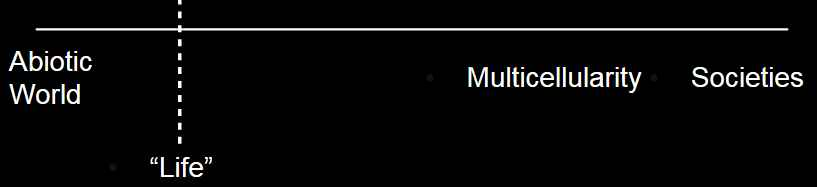
\includegraphics[width=0.9\textwidth]{lifesTransitions}
\end{figure}
At some point along this trajectory, we have this transition into something
that we would call life. How is it that we go from this
abiotic world to a biotic world, understanding that this is all part of one
evolutionary continuum. Why is that question so challenging?

Well, one of the things that makes it challenging is that it requires a lot of diverse types of knowledge to begin to understand this process and to answer this question;those types of knowledge draw from a variety of different disciplines--Figure \ref{fig:tradional:disciplines}.
\begin{figure}[H]
	\begin{center}
		\caption[Traditional disciplines needed for Origin of Life]{We need to understand something about Earth science, biology, chemistry, and physics and how all of these different concept areas intersect with one another and help us to understand exactly what happened when life first formed.}\label{fig:tradional:disciplines}
		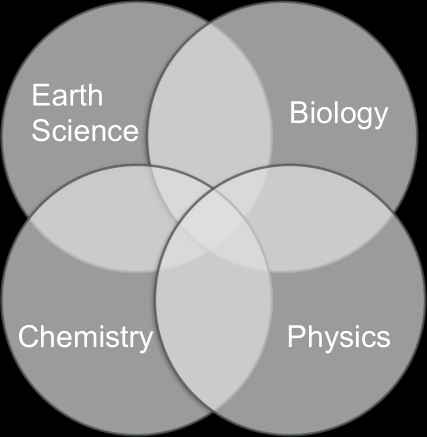
\includegraphics[width=0.9\textwidth]{4mainAreas}
	\end{center}
\end{figure}

Throughout this course, we will introduce you to the main questions in each of these concept areas and how they relate to the origins of life. And we will also start to begin to paint a picture of where the intersection and synthesis of these different concepts live, hopefully moving towards a better theory of how life started and evolved into greater complexity.

What are the main questions within these concept areas? 

\subsection{Earth Science}

\begin{itemize}
	\item What was the environment like during the time when life originated?
	We understand that the early Earth was 	very different from the modern Earth.
	\item What chemistry was possible on the early Earth? We need to understand something about what chemistry was possible then and how that might come together to help 	life form in the first place.
	\item What was the diversity and complexity of various micro-environments on the early Earth? If we think about the early Earth, not only as a different average chemical space from what we currently have, but	also having lots of different unique types of micro-environments in this very different planetary environment, which of those micro-environments were most likely to give us life in the first place or to have the right type of chemical complexity 	to at least start down that trajectory towards a living organism?
	
	\item How did early life and the geosphere co-evolve? 
	We understand, in the modern Earth, how life interacts with the overall planetary	system; we understand, through lots of the history of life how life interacts, has a large feedback width, and modifies	the geological environment and the geosphere. And the question is: when life first started, what did	that feedback look like and how did this coevolution happen, and how important was that for the	specific trajectory that life took once it was formed?
\end{itemize}


\subsection{Biology}
\begin{itemize}
	\item How do we wind the clock back from modern life to early life? From a biological perspective, the questions we're interested in are mostly how do we take everything we know about modern life and try to work as far back in time as we can? How do we wind back the clock on modern life to understand what early life might have looked like?
	This involves taking a lot of phylogenetic or genetic perspectives to
	look back in time.
	\item  What does the composition, structure, and function of modern life tell us about the origin?
	\item  Which aspects of extant life are general and which are arbitrary?
	\item How do we apply modern evolutionary theory to the proto-life? Also in that vein, how do we take everything we know about modern evolutionary theory and start to apply that to things like protolife which might have a much less formal version of
	inheritance or genetics.
	\item How can we use evolutionary theory to think about the simplest early life which
	might be radically different but also is almost certainly undergoing some sort of
	evolutionary process. So, what are the features that we see in 	modern life that are really essential to life through any origin and trajectory and 	which are contingent on the particular evolutionary history that we happened to
	have seen for more recent life?
\end{itemize}	


\subsection{Chemistry}
\begin{itemize}
	\item How does life arise from the huge space of chemical reactions and compounds? 
	We understand that chemistry gives us 	this really vast set of possibilities, 	this really rich high-dimensional space, which is great for allowing something 	like life to form but it makes it very complicated to understand exactly what combinations and processes and trajectories are actually necessary or were the ones that led to the life that we have.
	\item What was early “living” chemistry like? How was that possible in early Earth? How do 	we start to define sort of living chemistry that isn't quite life?
	\item How do we go from complicated chemistry in an environment to the amazing chemical complexity of even the simplest cells? Even the simplest cells have a set of chemistry and feedback and dynamics and interconnections that is much more 
	complicated than things that we see in the environment and so how do we make that
	transition?
\end{itemize}

	
\subsection{Physics}

\begin{itemize}
	\item How do physical constraints, such as the laws of thermodynamics, bound the possibilities for life? How do we take everything we know about physics and use that to say what is and 	isn't possible for life, especially for the	first forms?
	\item What properties and processes are ''easy'' to obtain through physical dynamics alone?	So for example, we understand that in 	purely physical systems, it's possible to get very rich pattern information and 	dynamics and so how much-- how important 	are those sorts of naturally emergent--	occurring phenomena to thinking about the first formation of life and how we start 	to apply some of those concepts of 	emergence and simple pattern formation to 	interact with
	how life began in the first place.
	\item How do we generalize physical concepts to understand life’s formation? How do we port physical concepts over 	to biology in general and in particular, how do we port those ideas over to the origins of life?
\end{itemize}	

As you can see this is a very rich set of questions coming out of a variety of concept spaces across a huge range of science and in this course we've gathered people from this wide diversity of scientific perspectives to really lay out the details of each of these questions in specific ways and then bring those details together in a way that we have a broader and more complete understanding of how life might have formed in the first place.


\section[Life]{Life--David Baum}

\subsection{Easy or hard?}
A key initial consideration is how easy, or hard, is it for life to emerge?
The extremes:
\begin{itemize}
	\item We need to wait billions of years for specific conditions: even hospitable planets lack life--Figure \ref{fig:luca}.
	\item New life can evolve quickly whenever conditions are ripe:  New life could emerge in the lab--Figure \ref{fig:zircons}.
\end{itemize}

Of course this isn't really a dichotomy, as there is a continuum from easy to hard.

\begin{figure}[H]
	\caption[Life is hard.]{Life is hard; Time is long. A key piece of evidence comes from looking at cellular life and tracing it back to a single ancestor--\gls{gls:LUCA}. If life were easy one might expect multiple independent trees.}\label{fig:luca} 
	\includegraphics[width=0.9\textwidth]{Luca}
\end{figure}

\begin{figure}[H]
	\caption[Life emerged quickly]{Life emerged quickly: The oldest rocks that could have retained evidence of life do have evidence of life. We now don't know any rock formation that doesn't have evidence of life. This figure depicts some inclusions in zircons\cite{bell2015potentially}, and the isotopic ratios suggest the carbon was from life.}\label{fig:zircons} 
	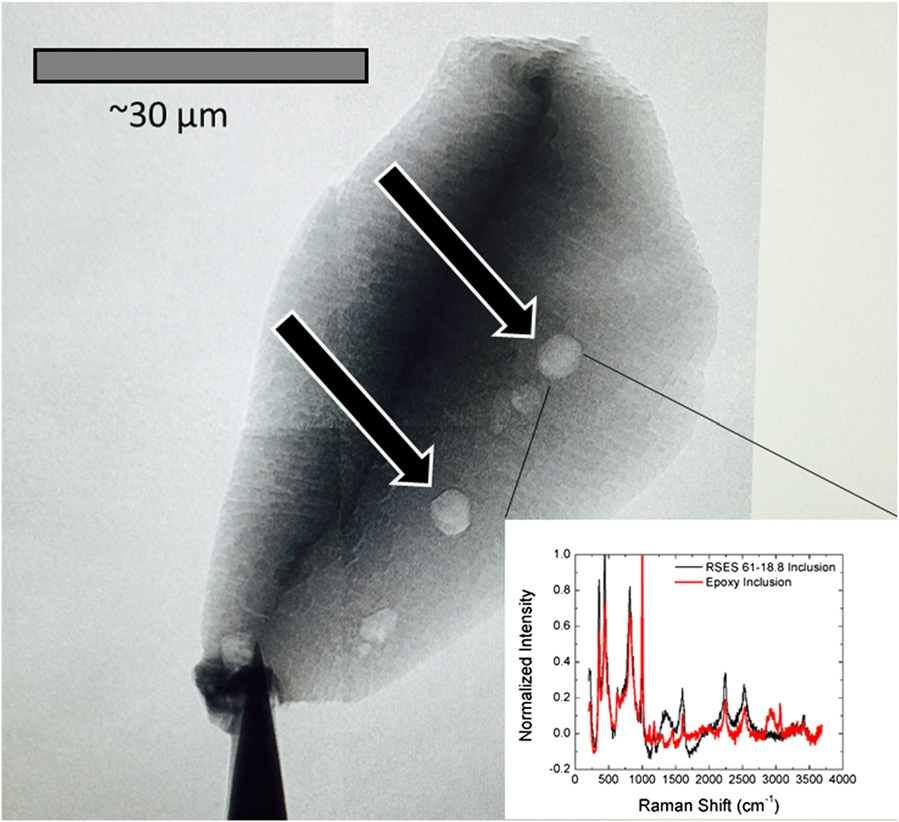
\includegraphics[width=0.9\textwidth]{Zircons}
\end{figure}

 Even if life arose only once, it nevertheless happened remarkably early, since Figure \ref{fig:zircons} dates from shortly after the planet had cooled enough to provide liquid water. To help us think about that we can turn to Charles Darwin.
\begin{itemize}
	\item Life pre-empts Life: \begin{quotation}
		But if (and oh! what a big if!) we could conceive in some warm little pond with all sorts of ammonia and phosphoric salts,—light, heat, electricity etc present, that a protein compound was chemically formed, ready to undergo still more complex changes, at the present day such matter would be instantly devoured, or absorbed, which would not have been the case before living creatures were formed--Charles Darwin\cite{darwin1871letter}. 
	\end{quotation}So the fact that life only emerged once does not necessarily mean that life is hard.
	
	\item Do we know that all life on this planet is cellular? Would we recognize alt-life?
	
	\item Some theories allow life to originate easily\cite{wachtershauser1988before}
\end{itemize}

\subsection{The meaning of ''life''}
In everyday discourse the term "life" is not ambiguous.
When we point at something and label it "alive," or an "instance of life," we usually know what we mean.
But, when it comes to the science and the philosophy of life, this is not so trivial.
And, in fact, scientists and philosophers have debated for a long time what we really mean by the term "life."

And, of course, we have a very clear reference point.
The reference point is cellular life--\gls{gls:LAWKI} on this planet,
which shares a number of distinctive features.
And, we can make a very long list of the features that all life as we know it share, and some of them are very specific.

\gls{gls:LAWKI} shares many features
\begin{itemize}
	\item They all use a nucleic acid code 	with the same bases-- (A,T/U,C, G)
	\item they all use the same 20 amino acids 	to make their proteins;
	\item they're always the left-handed variants.
	\item they will have a very similar genetic code,
	\item they all have similar machinery--ribosomes--for making proteins,
	\item they have similar biochemistry, (e.g. \gls{gls:ATP})
	\item they even share particular genes.
\end{itemize}

It's kind of exciting to realize that all life has these unique
and shared properties, because it tells us something fundamental about life as we know it, which is that life as we know it traces back to a single common ancestor--Figure \ref{fig:LUCA_common}.
\begin{figure}[H]
	\caption{Life as we know it traces back to a single common ancestor}\label{fig:LUCA_common} 
	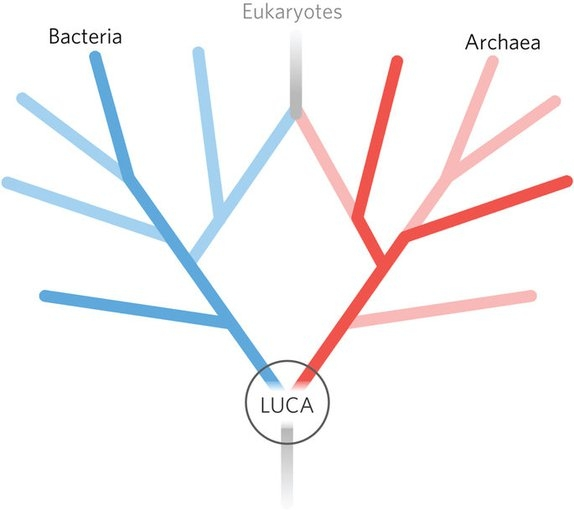
\includegraphics[width=\textwidth]{LUCA_common}
\end{figure}
So, there was, at some point in the past, an ancestral lineage that gave rise to
all three branches of life that we know of today--bacteria, archaea and eukaryotes.

And, the traits that we see in all life as we know it--that list I just gave you and more--all predate the last universal common ancestor, the last organism that was ancestral to all three of those lineages.
So, that's an exciting and important insight, but it also poses a slight problem, which is--life as we know it has a very long list of shared traits.
But, it doesn't necessarily guide us as to ask the question--suppose you found some other lifelike system,maybe on another planet or in some strange environment,you wanted to decide--''Is this thing alive? Is it an instance of life?''--you presumably wouldn't care about this full laundry list.These particular traits are the result of the historical factors that occurred in the origins of this life. and we want some more general understanding of life to answer the question - is something else another instance of life?

So, people have tried to approach this by whittling down those specific traits
to generalities -- general features -- that life seems to have
that distinguish these instances of life from instances of non-life --
inanimate matter. And if, you open any sort of biology textbook, you'll have a list of the features of life, and they vary in number from five, seven, eight, whatever--Figure \ref{fig:lawki-focus}.

\begin{figure}[H]
	\caption{Focus on generic features...but which?}\label{fig:lawki-focus} 
	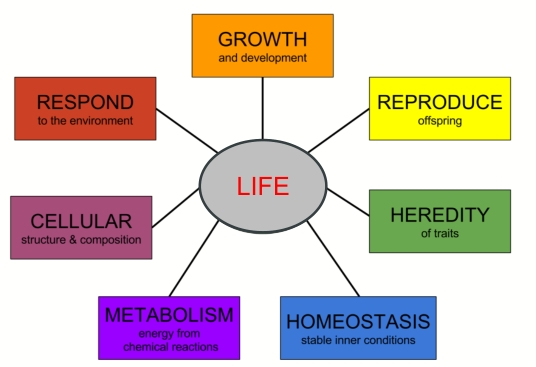
\includegraphics[width=\textwidth]{lawki-focus}
\end{figure}
And, this has been the starting point for a process in the origin of life field of thinking about - how low can we go? 
What, at core, are the essential features of something to be considered to be an instance of life in the general sense?

Now, there might be some difference of opinion, but, by and large, the field has converged on two key features, which are captured in this definition I've given here.
\gls{gls:life} is \glsdesc{gls:life}.

This definition is based on one that was kind of established by NASA to help guide them in the question of looking on other planets and deciding whether there is life there.

\begin{itemize}
	\item life is a self-propagating chemical system, meaning it's a system that makes more of itself over time--or least can;
	\item  we expect  that this system 	is capable of undergoing
	adaptive evolution--Figure \ref{fig:AdaptiveEvolution}.
	\item \emph{self-propagation} and \emph{evolution} are key
\end{itemize}

So, let's look at those two pieces in turn.


The idea of self-propagation is that you have some kind of chemical system that can make more of itself and occupy additional areas of space. It doesn't much matter whether we're thinking about growth, which is where we have a single, living protoplasm that expands to encompass more space, or if we're thinking about the process of making multiple cells from a single parent cell.
The only difference between these phenomena is whether or not the newly formed protoplasm--living material --either is not sort of packaged up into cells.
And so, what we expect of anything that we would label to be "alive"--is that it has some capacity to propagate itself spatially.
But, of course, that isn't really enough because we know of quite a few systems that can self-propagate,
but we usually wouldn't call them "alive"--for example, a crystallization process.
\begin{figure}[H]
	\caption[Adaptive Evolution]{Adaptive evolution entails the potential to complexify and become more out-of-equilibrium. Surface \gls{gls:protoplasm} ulimately evolves to a \gls{gls:protocell}, as described in \cite{baum2015selection}}\label{fig:AdaptiveEvolution} 
	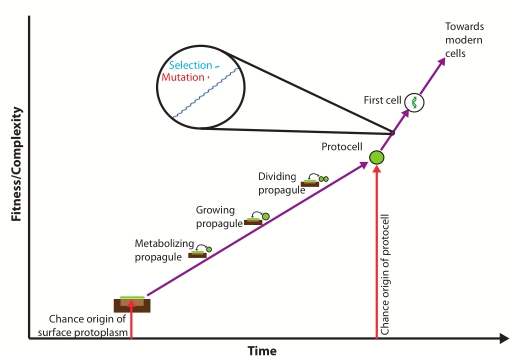
\includegraphics[width=0.9\textwidth]{AdaptiveEvolution}
\end{figure}

And, that's where the second part
of the definition comes in -
and that is this idea that things
that we want to consider to be alive
also have the capacity
for adaptive evolution...
which means that
they have the capacity
to get better at
self-propagating over time.
This is an important idea
and something that we don't see in,
for example, crystallization processes,
because it explains
how it is that life as we know it
became so complicated
and out of equilibrium
with their chemical environments.
Cells and living systems that we know
are quite sophisticated
and certainly far from being typical of
the chemical environment around them.
And, this is possible because,
during the adaptive process,
the variants arise,
and the fate of those variants
is independent of whether they are
of raised or lower complexity.
Natural selection,
the driving force of adaptive evolution,
will select the trait that
confers higher fitness
whether or not
it's a more complicated trait.
Furthermore, there are many instances
in which we know
that the more complicated variants
have an advantage.
As a result,
over long, long periods of time,
adaptive evolution can explain
how a simple self-propagating system
can become more and more complex.

So, putting these
two pieces together,
it's fair to say that
the origin of life field,
in general, has a great deal
of attention...
that it pays to these two properties -
self-propagation and adaptive evolution.
We try and understand
how they come about,
and we try and understand the kinds
of planetary or chemical conditions
in which we might expect
self-propagation and evolution
to emerge spontaneously.



\section[Constraining Chemical Complexity to Form Life]{Constraining Chemical Complexity to Form Life--Zach Adam}

We'll be talking about huge chemical complexity, and constraining the complexity to form life. When we look at the deep past we find some interesting challenges regarding how life could have originated from a non-living environment. Most matter isn't alive: how to bridge the two states of matter?

\begin{figure}[H]
	\caption{Chemical Complexity}\label{fig:ChemicalComplexity} 
	
	\begin{subfigure}[b]{0.45\textwidth}
		\centering
		\caption{When we first learn chemistry, we use stick and ball model}
		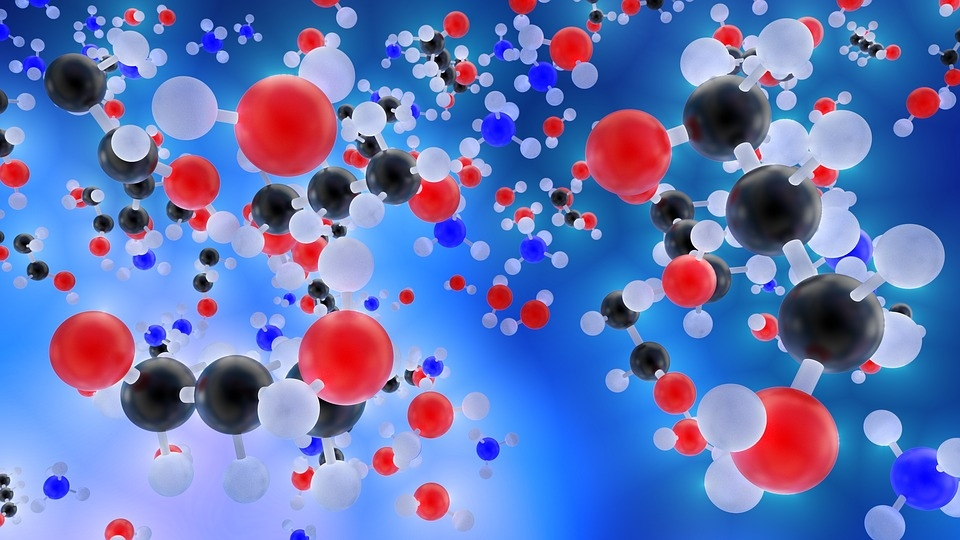
\includegraphics[width=\textwidth]{ChemicalComplexity}
	\end{subfigure}
	\begin{subfigure}[b]{0.45\textwidth}
		\centering
		\caption{But atoms really have many levels, all interacting. The outer layers of electrons give rise to the "sticks" in the na\"ive model.}
		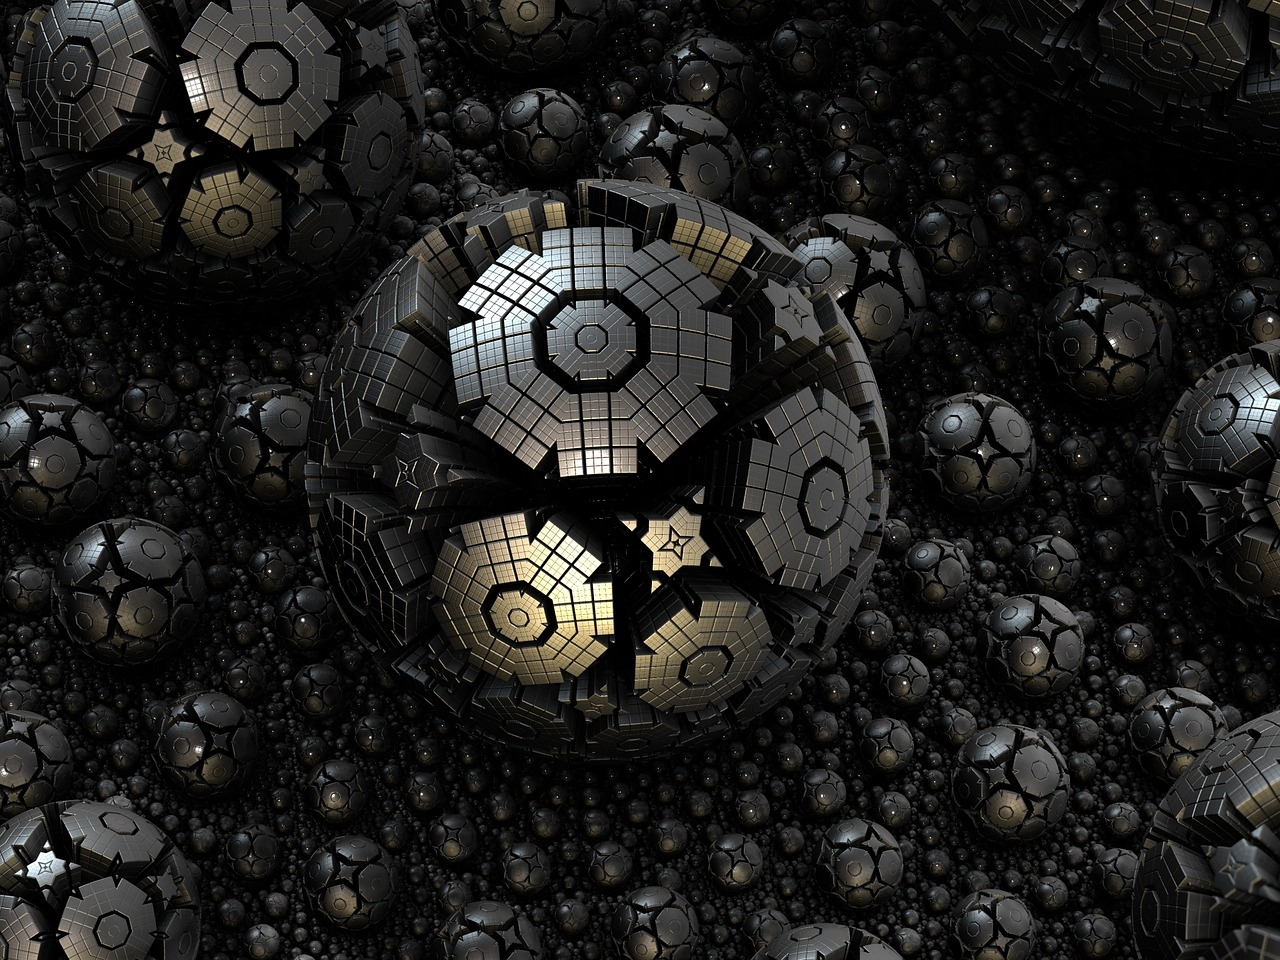
\includegraphics[width=\textwidth]{ChemicalComplexity1}
	\end{subfigure}
\end{figure}

Let's start with a canonical type of molecule--Figure \ref{fig:NucleotideMolecule}. When we zoom in a bead we see that it represents three molecules. If we change even one atom, or link the atoms differently, the molecule may not function.
\begin{figure}[H]
	\caption{Nucleotide Molecule }\label{fig:NucleotideMolecule}
	
	\begin{subfigure}[b]{0.45\textwidth}
		\centering
		\caption{RNA Molecule: one bead expands to 3 molecules. Change one atom, likely to change behaviour of entire molecule!}
		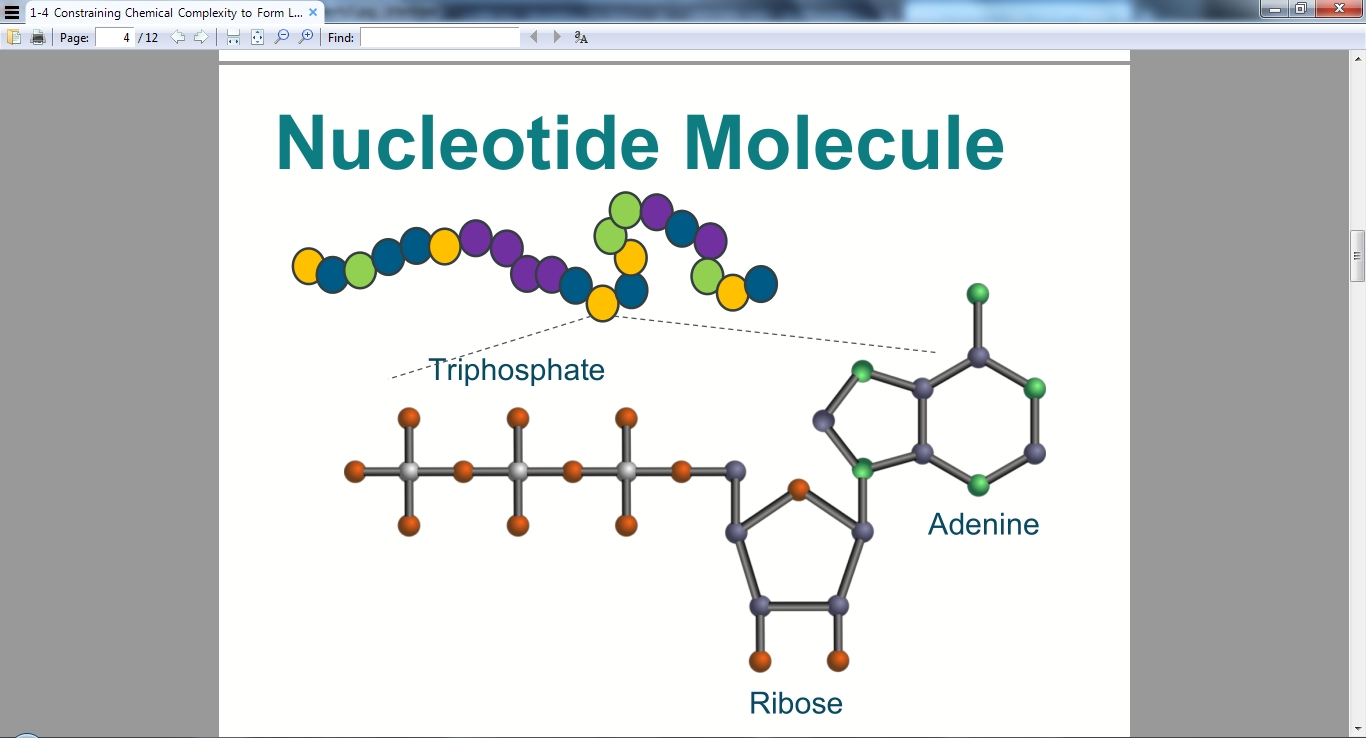
\includegraphics[width=\textwidth]{NucleotideMolecule}
	\end{subfigure}
	\begin{subfigure}[b]{0.45\textwidth}
		\centering
		\caption{Zoom into Adenine Molecule: change one thing, not adenine any more!}\label{fig:adenine}
		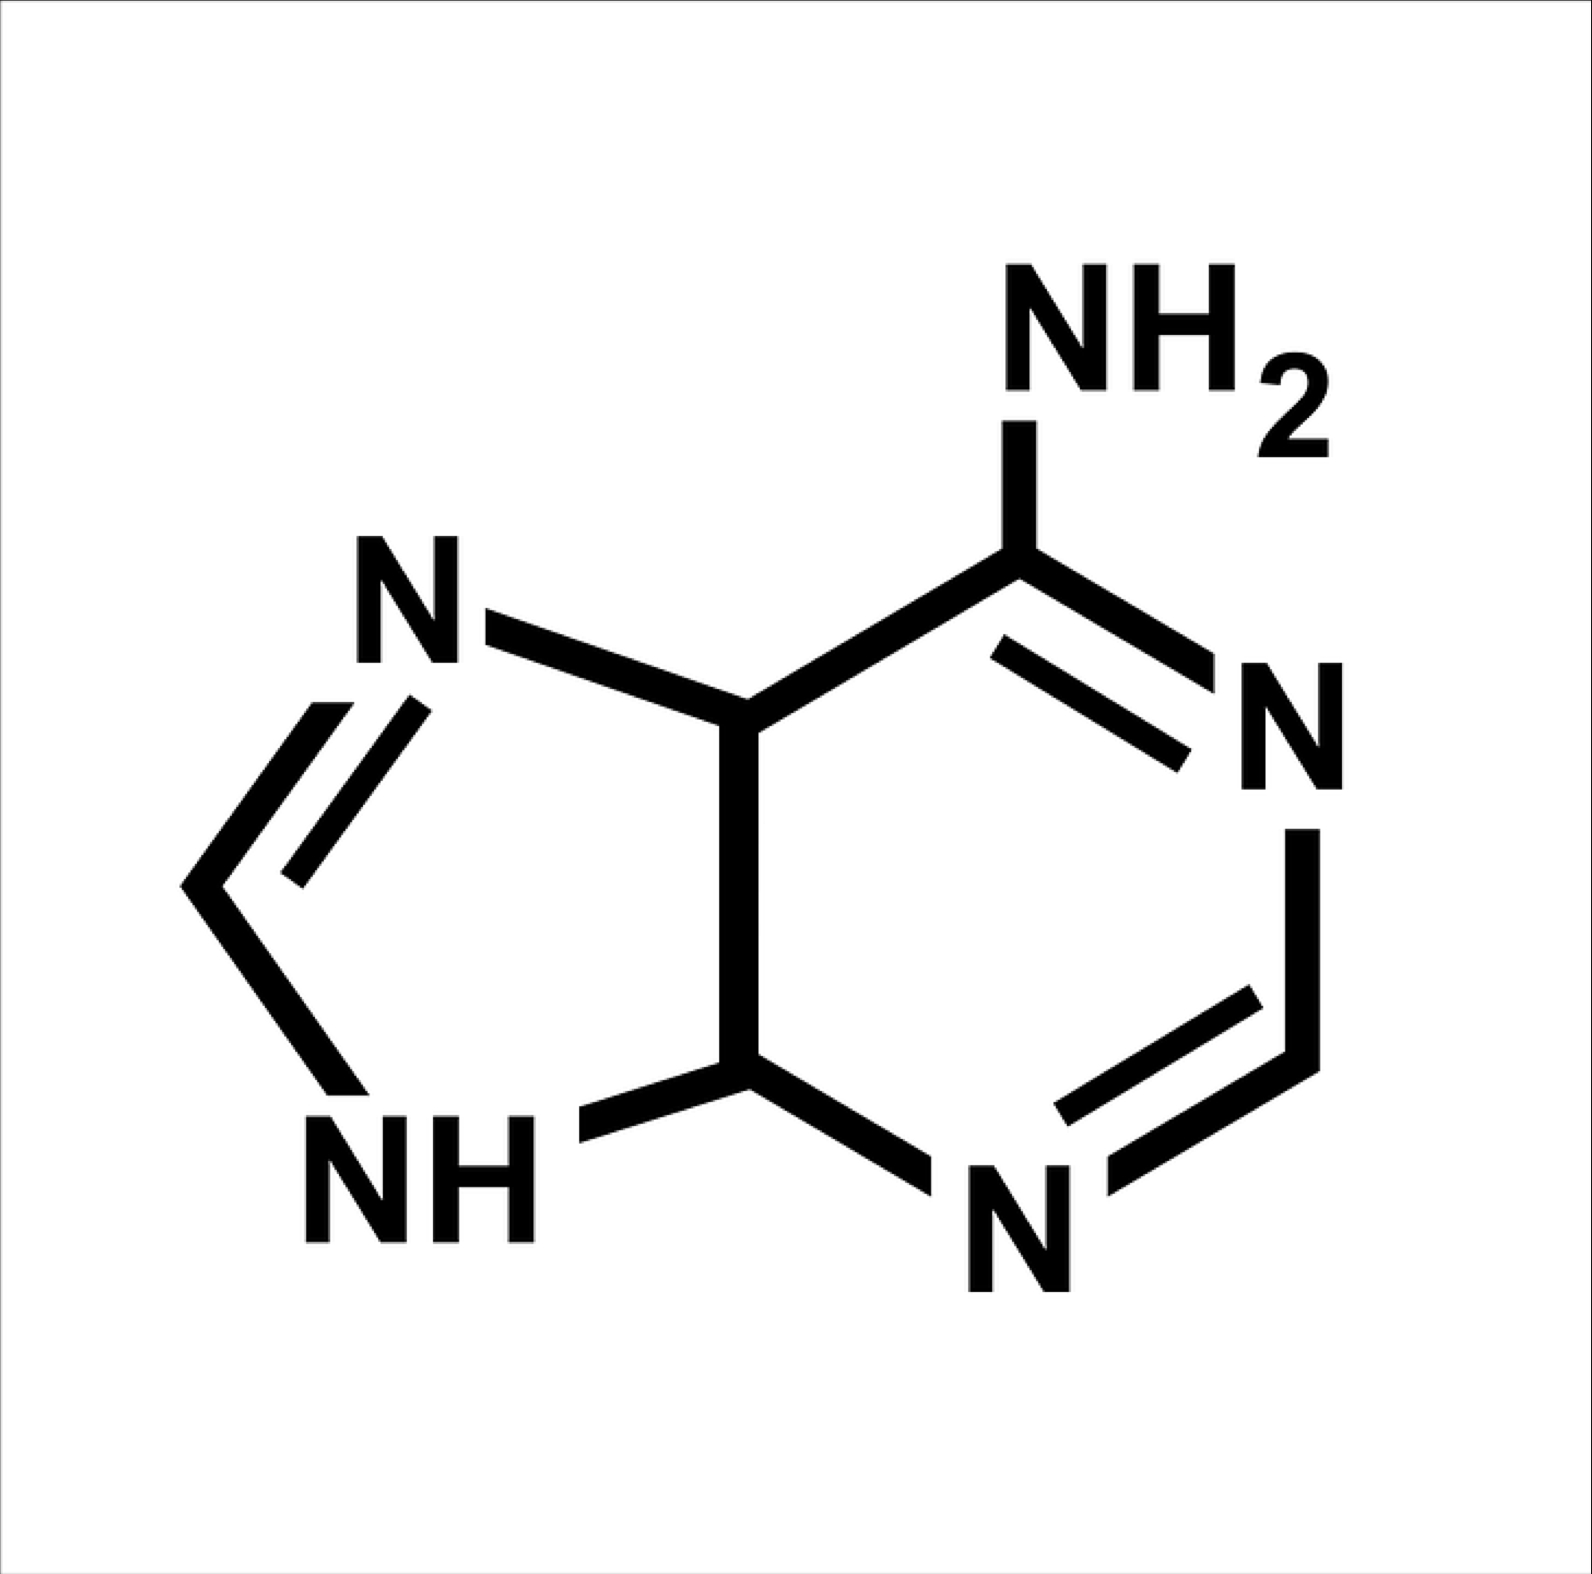
\includegraphics[width=0.6\textwidth]{AdenineMolecule}
	\end{subfigure}
\end{figure}

Let's zoom in further on the Adenine molecule, Figure \ref{fig:adenine}: change any atom and it wouldn't be adenine; now zoom in even further, Figure \ref{fig:MolecularInteractions}, and we see more interactions between atoms and with solvent.

\begin{figure}[H]
	\begin{center}
		\caption[Zoom in further, and atoms interact with each other]{Zoom in further, and atoms interact with each other, and with solvents!}\label{fig:MolecularInteractions} 
		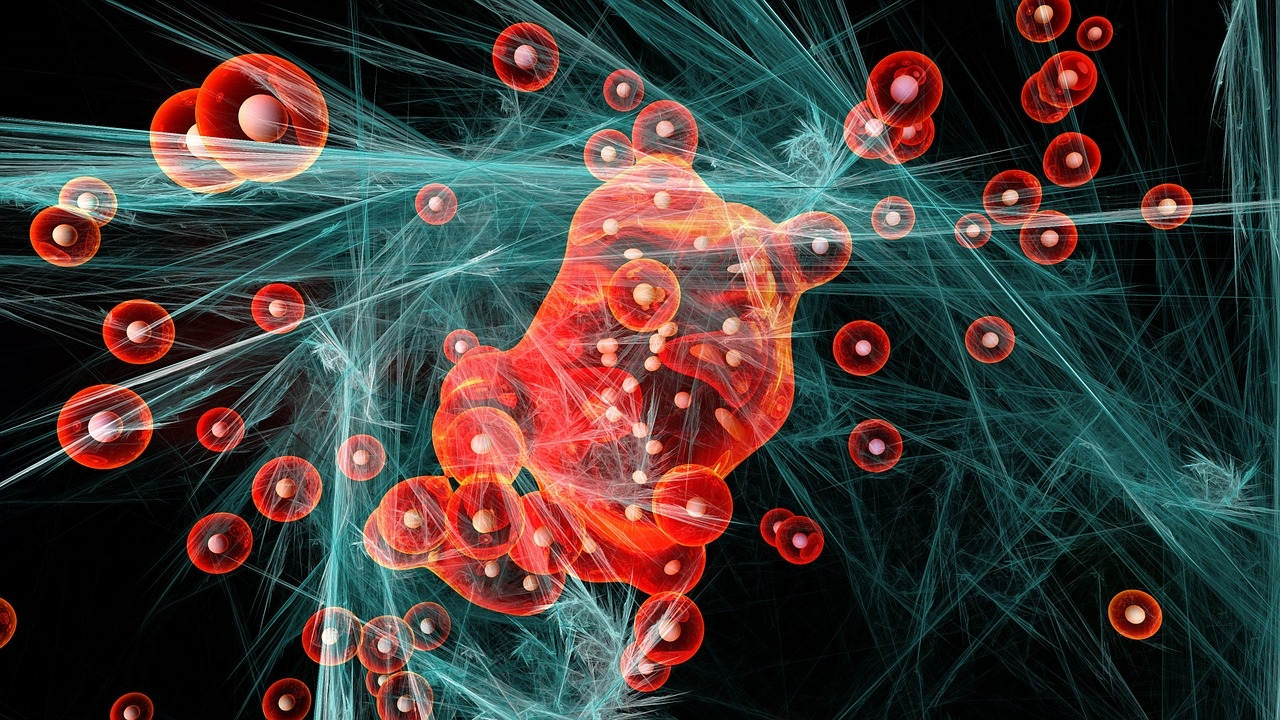
\includegraphics[width=0.9\textwidth]{MolecularInteractions}
	\end{center}
\end{figure}

If you want to think about generating these molecules from scratch, you need to think about all these interactions and their effects.

There are a number of ways origins of life researchers try to navigate this complexity and design experiments that get to the root of how life could have originated from a non-living state.

\begin{itemize}
	\item Constrain Location 
	\begin{itemize}
		\item Advantages
		\begin{itemize}
			\item Many possibilities for complex interactions
			\item Experiments can be designed by analogy with modern environments.
		\end{itemize}
		\item Disadvantages: mostly implausible to assume pure reactants in natural settings
	\end{itemize}
	\item Constrain Reactants
	\begin{itemize}
		\item Advantages: limit to needed molecules and needed amounts.
		\item Disadvantages: resulting network is not very complex or robust
	\end{itemize}	
	\item Constrain Energy Sources
		\begin{itemize}
		\item Advantages: processes are not location- or reactant-specific; many 		outcomes are possible
		\item Disadvantages: Difficult or impossible to predict outcomes of
		processes that cross multiple object levels
	\end{itemize}
\end{itemize}

Examples
\begin{itemize}
	\item Constrained Location Examples \begin{itemize}
		\item Hydrothermal Vents\cite{martin2006origin}
		\item Atmosphere (Impactor/Shock Synthesis, Lightning,
		Insolation)\cite{chyba1992endogenous} \cite{miller1959organic}
	\end{itemize}
	\item Constrained Reactant Examples 
	\begin{itemize}
		\item RNA World\cite{powner2009synthesis},
		\item Pyrite-mediated synthesis\cite{wachtershauser1993cradle}
		\item Borate-mediated synthesis\cite{grew2011borate}
	\end{itemize}
	\item Constrained Energy Examples
	\begin{itemize}
		\item \Gls{gls:serpentinization}\cite{schrenk2013serpentinization}
		\item Solar flares\cite{airapetian2016prebiotic}
		\item Radioactivity\cite{yi2018radiolytic} \cite{adam2018estimating}
	\end{itemize}
\end{itemize}

\section[Geological Conditions, Change, and Chaos]{Geological Conditions, Change, and Chaos--Zach Adam}

What is the source of our understanding of conditions when we thought life originated?
\begin{figure}[H]
	\caption[Earth's Structure]{Earth's Structure: includes everything in Figure, plus minerals, etc. We can only sample surface, plus a few km  down.}\label{fig:EarthStructure} 
	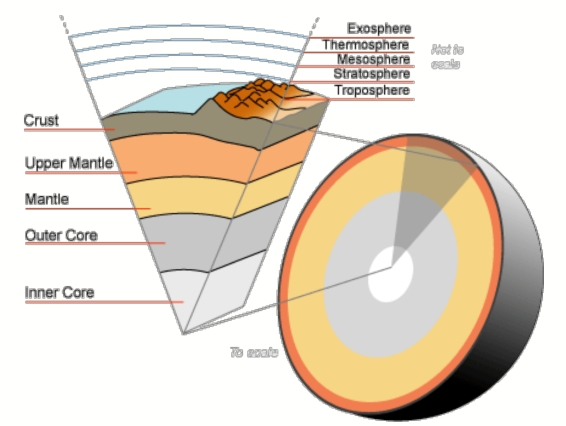
\includegraphics[width=0.9\textwidth]{EarthStructure}
\end{figure}

Continents don't stay in the one place. So what we say today may not be what was there in the past.
\begin{figure}[H]
	\caption{Geologic Record is inseparable from history of life}\label{fig:GeologicRecord} 
	
	\begin{subfigure}[b]{0.45\textwidth}
		\centering
		\caption{Great oxidation event changed all sorts of stuff. We need oxygen, but other critters had to adapt or die. Oxidation changed minerals.}
		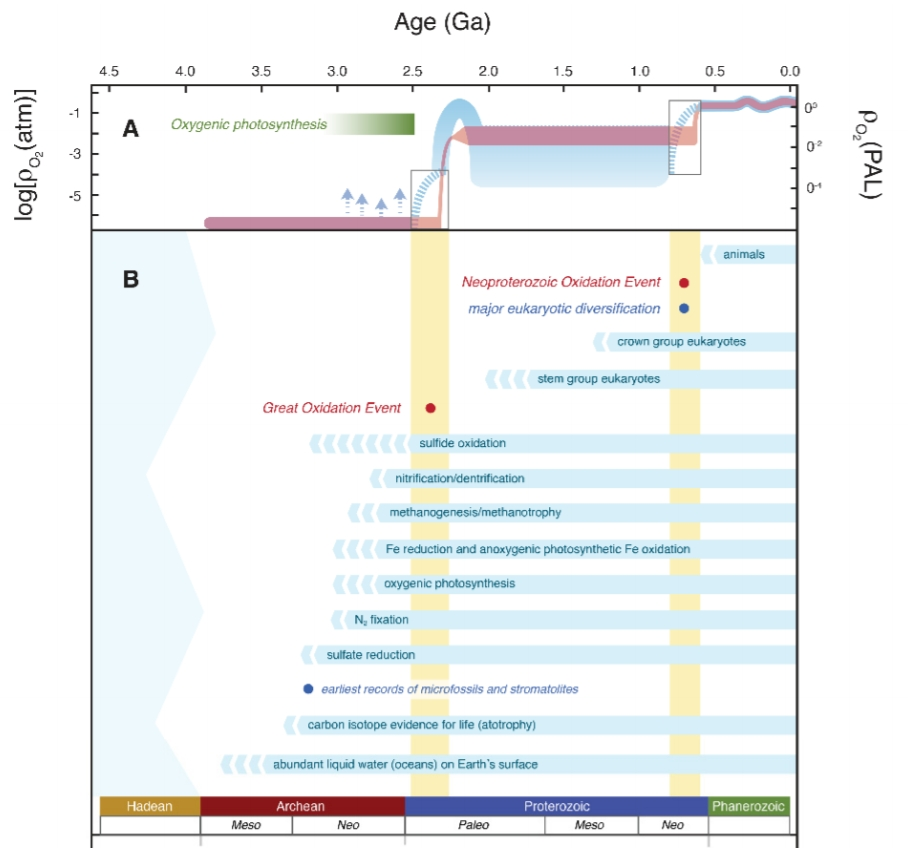
\includegraphics[width=0.8\textwidth]{GeologicRecord}
	\end{subfigure}
	\begin{subfigure}[b]{0.45\textwidth}
		\centering
		\caption{How much change has been caused by weathering? There are different models for crustal accumulation. So how much crust has been produced over time?}
		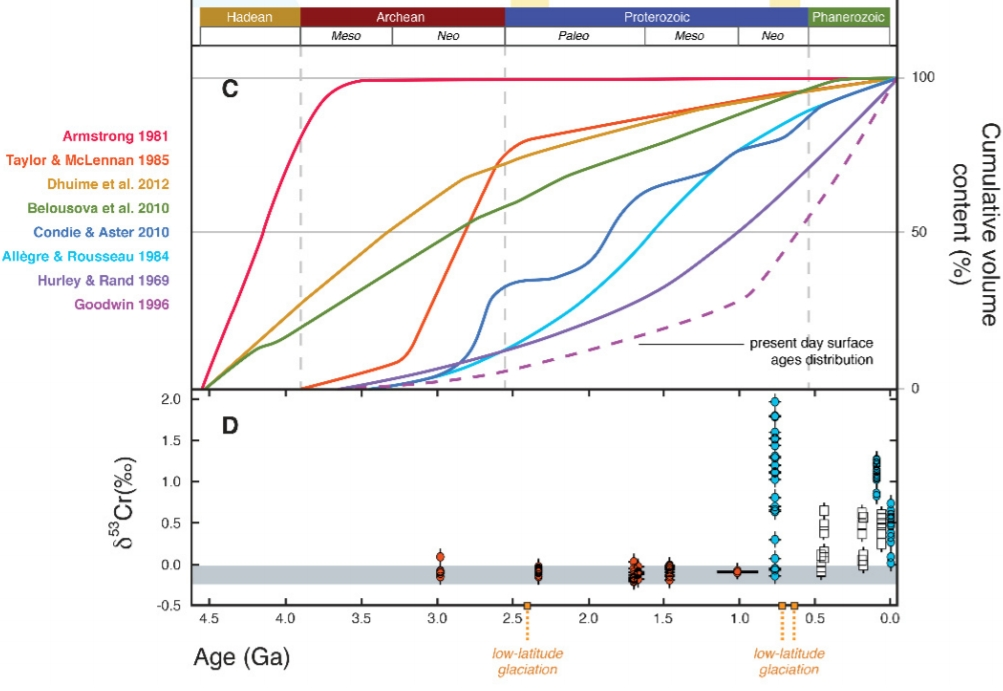
\includegraphics[width=\textwidth]{GeologicRecord1}
	\end{subfigure}
\end{figure}

\begin{figure}[H]
	\caption[Another Level Down: different models for accumulation of crust.]{Another Level Down: different models for accumulation of crust. Not simple accumulation! There may have been periods where there was more crust than today\cite{spencer2017growth}.}\label{fig:AnotherLevelDown} 
	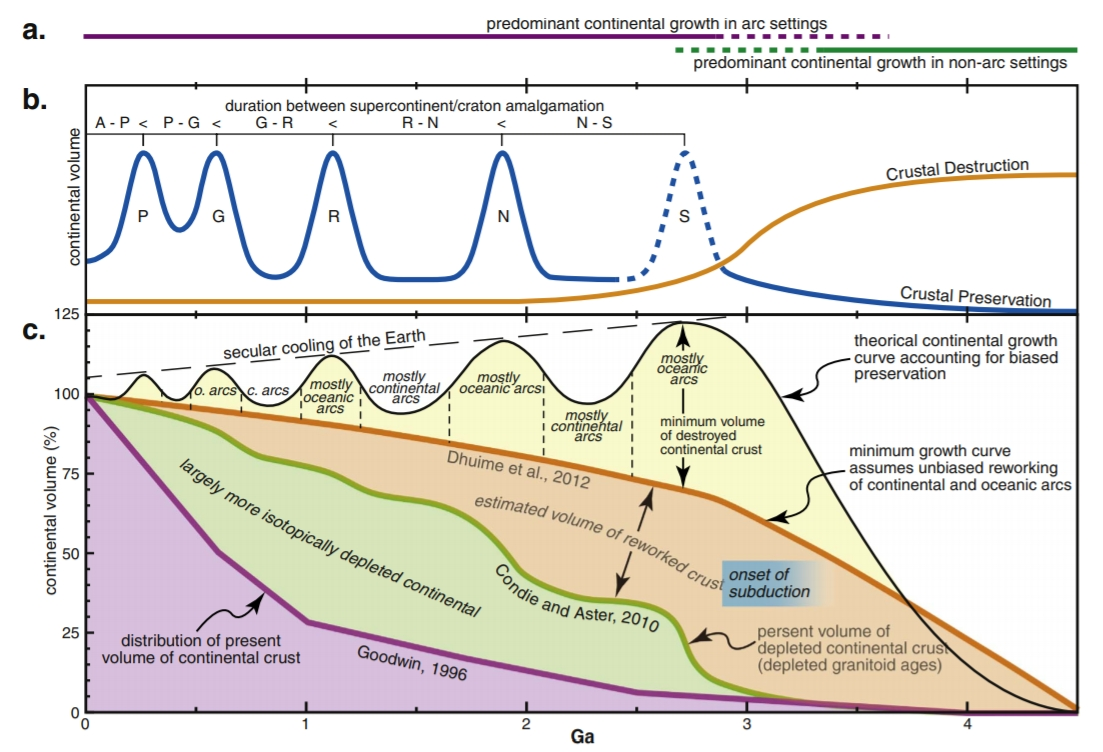
\includegraphics[width=0.9\textwidth]{AnotherLevelDown}
\end{figure}

Only direct record for events that sow chaos and processes of prolonged gradual change; much of the evidence for such events may have been lost.

What does this mean for origins of life research?
\begin{itemize}
	\item Limited direct rock data
	\begin{itemize}
		\item 	Sampling and preservation
		biases abound!
			\item No rock packages to
		provide environmental
		context or views into surface
		conditions.
		\item 	No rocks and few minerals
		from time surrounding life’s
		origins.
	\end{itemize}
	\item Complementary lab data
	\begin{itemize}
		\item Experiments are critical for
		filling in where the rock
		record is not available.
			\item Unclear whether powerful
		events/energy are more
		constructive than destructive.
	\end{itemize}
\end{itemize}

\section[Pattern Formation in Chemical Systems]{Pattern Formation in Chemical Systems-- Chris Kempes}

\begin{itemize}
	\item What properties and processes are easy to obtain through physical dynamics alone?	
	\item How might this make it easy for lifelike things to begin?
\end{itemize}

We will look at pattern formation through the lens of Reaction Diffusion Equations\cite{sfi_grayscott2018}.

Here is a very simple reaction diffusion equation. It relates the change in concentration of some chemical,  $U$, to a diffusion plus a reaction.
\begin{align*}
\frac{\partial U}{\partial t} =&   \underbrace{\overbrace{D_V}^\text{diffusivity} \underbrace{ \nabla^2 U }_\text{difference in fluxes}}_\text{diffusion term} + \underbrace{ F(U)}_\text{reaction term}
\end{align*}

With two chemicals...
\begin{align*}
\frac{\partial U}{\partial t} =&   D_U \nabla^2 U + F(U,V)\\
\frac{\partial V}{\partial t} =&   D_V \nabla^2 V + G(U,V)
\end{align*}

Now let's consider a specific example.
Consider two reacting species, $U$ and $V$, and an inert product $P$.
\begin{align*}
U + 2V \Longrightarrow& 3V\\
V \Longrightarrow& P
\end{align*}

\begin{enumerate}
	\item The first term in (\ref{eq:U}) represents the reaction of $U$ with $2V$. 
	\item We have chemostated the system, meaning there is some constant flux into the system and out of the system. $F(1 - U)$ represents flow in and out.
	\item Middle term in (\ref{eq:V}) represents outflow of $V$ plus conversion to $P$.
\end{enumerate}
\begin{align*}
	\frac{\partial U}{\partial t} =& -U V^2 + F(1 - U)  + D_u \nabla^2 U \numberthis \label{eq:U}\\
	\frac{\partial V}{\partial t} =& U V^2 - (F +k) V + D_v \nabla^2 V \numberthis \label{eq:V}
\end{align*}

This set of equations gives rise to very interesting spatial patterns. Using stability analysis we can determine the range of $F$ and $k$ that allow interesting patterns to form--Figure \ref{fig:GreyScottRange}.

\begin{figure}[H]
	\caption{Grey Scott Reaction}
	\begin{subfigure}[b]{0.3\textwidth}
		\centering
		\caption{the range of $F$ and $k$ that allow interesting patterns to form.}\label{fig:GreyScottRange}
		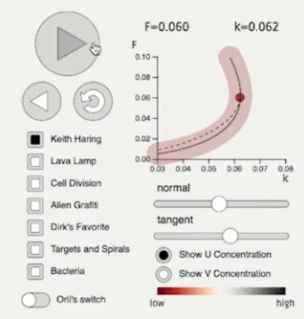
\includegraphics[width=\textwidth]{GreyScottRange}
	\end{subfigure}
	\begin{subfigure}[b]{0.3\textwidth}
		\centering
		\caption{Starting configuration}
		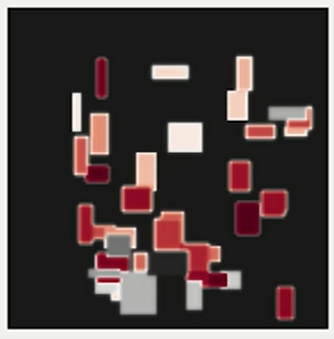
\includegraphics[width=\textwidth]{GreyScottInitial}
	\end{subfigure}
	\begin{subfigure}[b]{0.3\textwidth}
		\centering
		\caption{Evolves toward steady state,  where high concentration close to low concentration.}
		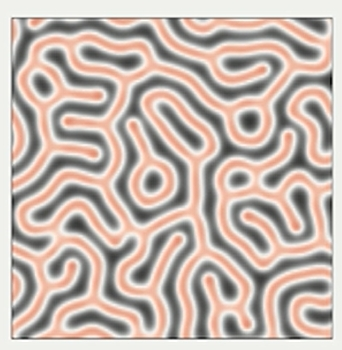
\includegraphics[width=\textwidth]{GreyScottFinal}
	\end{subfigure}
\end{figure}

What is very nice about this is it tells us that in a very simple context where we are combining this reaction with diffusion we see this very interesting pattern formation with strong spacial gradients: very high concentrations of $U$ and $V$ are separated by small distances and we see segregation. We can get very different concentrations very close to one another. This gives us hope, from an origins of life point of view, of getting complicated chemistry forming close to other complicated chemistry on small spatial scales in a way that is stable and segregated. 

Other starting values give cell-like behaviour (including division), so maybe get some ''lifelike" behaviour from physics and simple chemistry.

\section[The Central Dogma of Biology]{The Central Dogma of Biology--Chris Kempes}


\subsection{The Central Dogma of Biology}

One of the overarching questions of this class is how do we unwind present day life to learn about origins? Focus on most common properties of all life, especially the Central Dogma.\cite{crick1958biological} \cite{crick1970central}

\begin{figure}[H]
	\caption[The Central Dogma]{The Central Dogma after \cite{crick1970central}}\label{fig:CentralDogma} 
	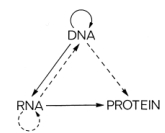
\includegraphics[width=0.9\textwidth]{CentralDogma}
\end{figure}


\begin{figure}[H]
	\caption[Ribosome is conserved across life]{Ribosome is conserved across life, but appears to have onion structure, built up by evolution. Ribosome started with common core, and more added.\cite{hsiao2009peeling}.}\label{fig:Ribosome} 
	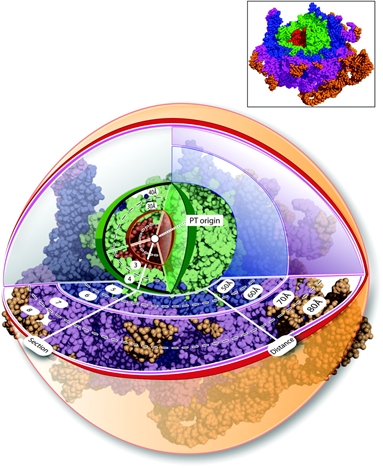
\includegraphics[width=0.9\textwidth]{Ribosome}
\end{figure}
Williams argues that we can use the onion, Figures \ref{fig:Ribosome} and \ref{fig:RibosomePhases}, to unwind evolution.

\begin{figure}[H]
	\caption[Ribosome Phases]{Ribosome Phases after \cite{petrov2015history}, illustrating evolution of  \gls{gls:LSU} and \gls{gls:SSU}}\label{fig:RibosomePhases} 
	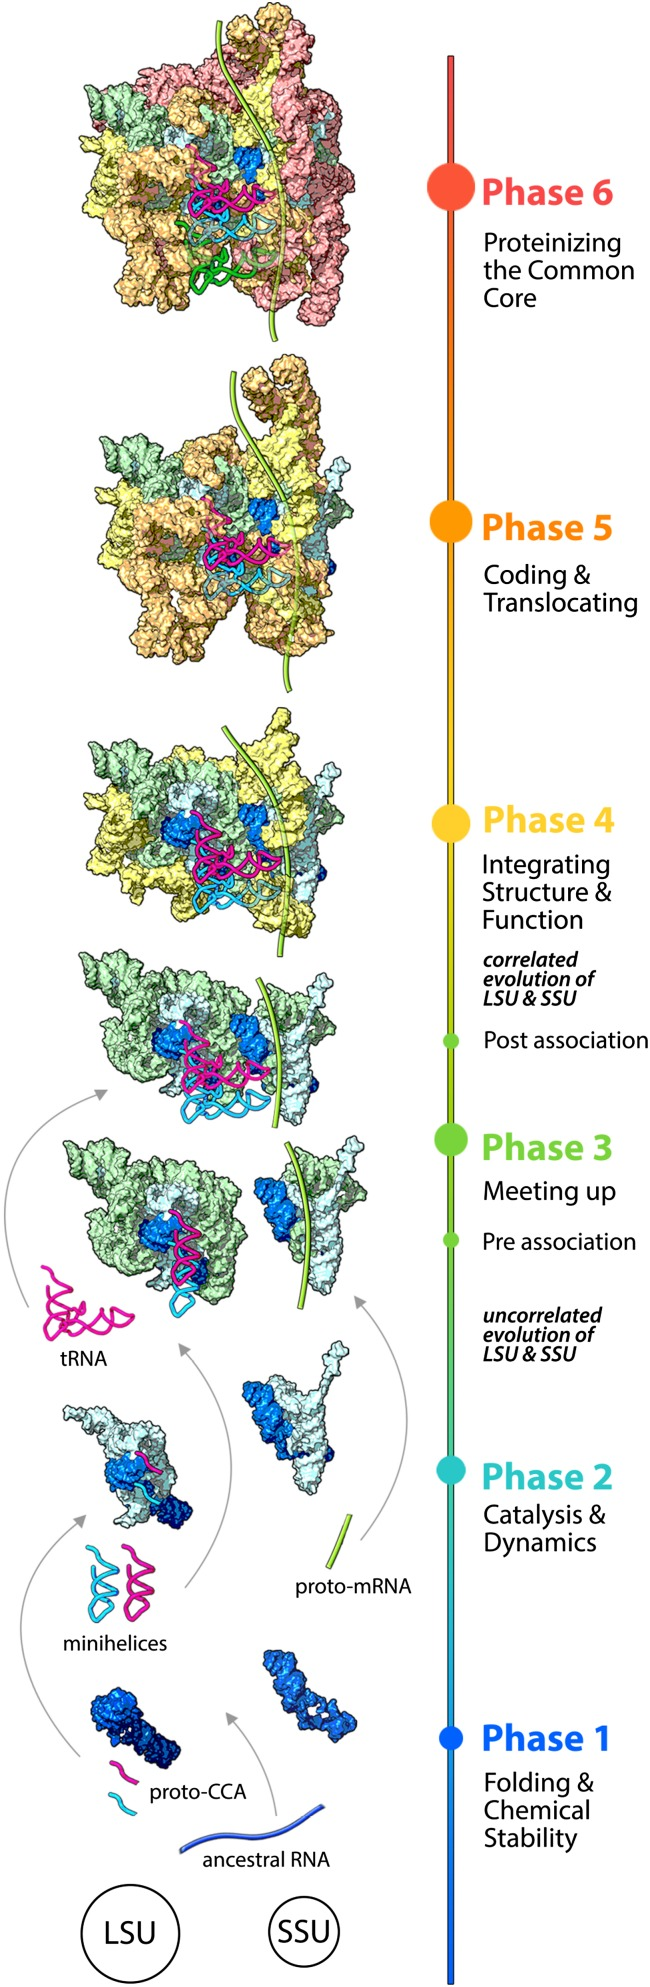
\includegraphics[width=0.5\textwidth]{RibosomePhases}
\end{figure}

Carl Woese used this to build new a Tree of Life.

\begin{figure}[H]
	\caption[Tree of Life]{\gls{gls:TOL}\cite{nair2012woese}}\label{fig:TOL} 
	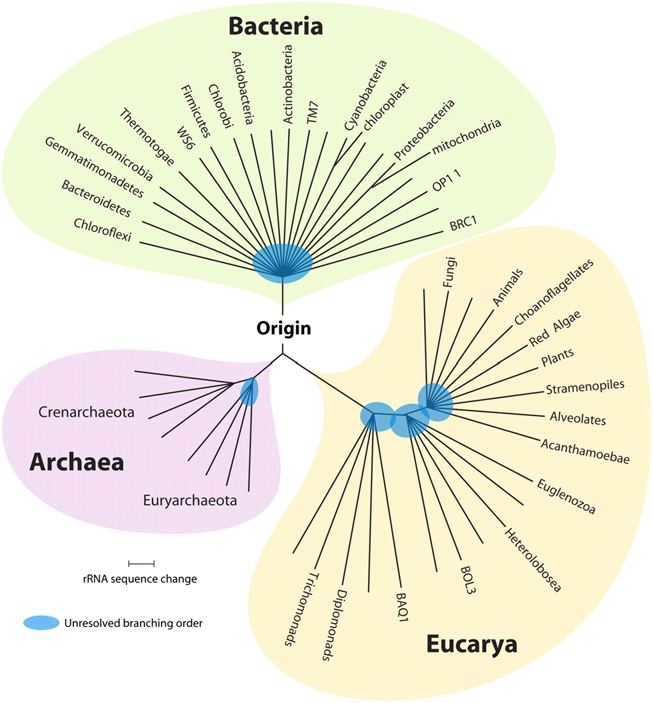
\includegraphics[width=0.9\textwidth]{TOL}
\end{figure}

\subsection{The Efficiency of the Central Dogma of Biology}

\gls{gls:landauer_bound}: \glsdesc{gls:landauer_bound}. 

\begin{figure}[H]
	\caption[Take unordered set of letters and try to write as specific string]{Take unordered set of letters and try to write as specific string\cite{kempes2017thermodynamic}}\label{fig:LandauerRibosome} 
	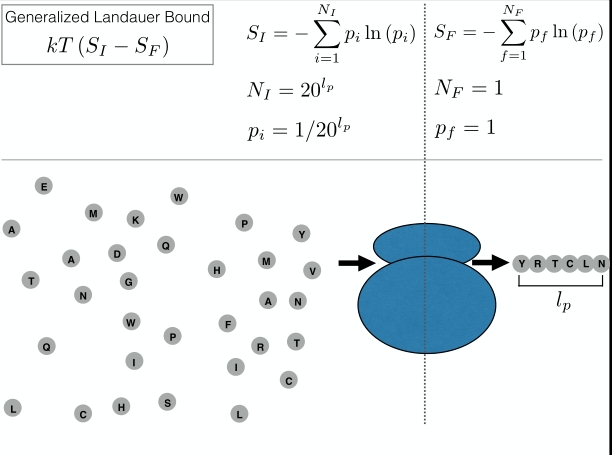
\includegraphics[width=0.9\textwidth]{LandauerRibosome}
\end{figure}

\begin{itemize}
	\item Life is only 20 times less efficient that physical limit\cite{kempes2017thermodynamic}
	\item Computers are 100,000,000 times worse than Landauer's bound!
\end{itemize}

\begin{figure}[H]
	\caption{Ribosome Tradeoffs}
	\begin{subfigure}[b]{0.45\textwidth}
		\caption{For a small cell, DNA and proteins take up (nearly) entire volume; for large cells, Ribosome does same thing! So we have bounds on allowable volume.\cite{kempes2016evolutionary}}\label{fig:RibosomeTradeoffs} 
		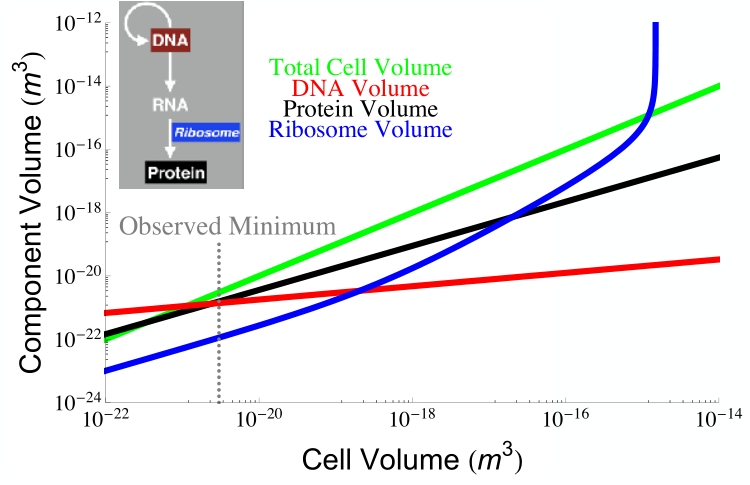
\includegraphics[width=\textwidth]{RibosomeTradeoffs}
	\end{subfigure}
	\;\;\;
	\begin{subfigure}[b]{0.45\textwidth}
		\caption{A more efficient ribosome would allow larger cells; less efficient might not work at all.}\label{fig:RibosomeTradeoffsEarly} 
		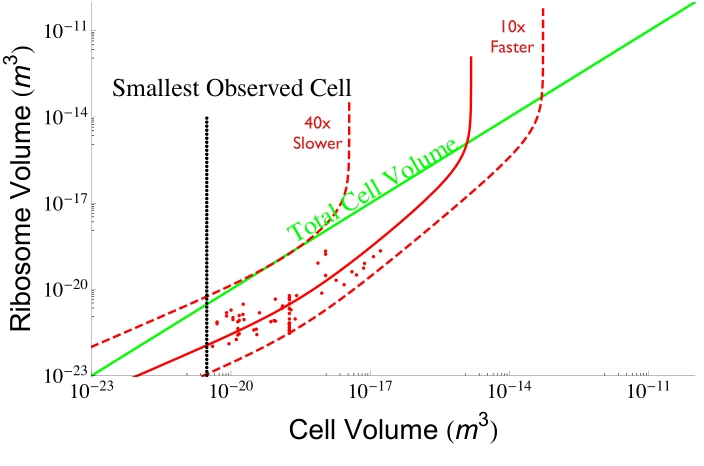
\includegraphics[width=\textwidth]{RibosomeTradeoffsEarly}
	\end{subfigure}
\end{figure}
\section[Biological Similarity]{Biological Similarity--Sarah Mauer}

We will use a top-down approach.

 ''By examining and deconstructing the commonalities between modern living organisms, we can better understand the requirements of first life.''

\begin{itemize}
	\item \Gls{gls:chirality}--Figure \ref{fig:Chirality}
	\begin{itemize}
		\item L-amino acids for all proteins;
		\item D-sugars for all sugars and nucleic acids.
	\end{itemize}
	\item The next thing that all living organisms have in common
	is that they use membranes to separate themselves from the environment--Figure \ref{fig:Membranes}--and these membranes are composed of amphiphilic molecules which have two parts:  a hydrophobic tail that aggregates between itself and a hydrophilic head group that interact with the water phase. This creates a barrier to the environment and also helps to keep important molecules inside the cell.
	Many/membranes are used to separate cells from one another they are also used
	to separate \glspl{gls:organelle} from other parts of the cell;
	one organelle is the nuclear membrane which separates the nucleic acid from the \gls{gls:cytosol}.
	\item The nucleic acids are another component that all living things have in common. The small chemical structures that you see here are very highly conserved between all nucleic acids. DNA similarities:\begin{itemize}
		\item little difference in chemical structure between organisms
		\item some difference in packing
		\item large difference in the size of genome
	\end{itemize}
	\item All cells use proteins, made from the same 20 amino acids.
\end{itemize}

\begin{figure}[H]
	\caption[L-amino acids and D-sugars]{L-amino acids for all proteins; D-sugars for all sugars and nucleic acids}\label{fig:Chirality}
	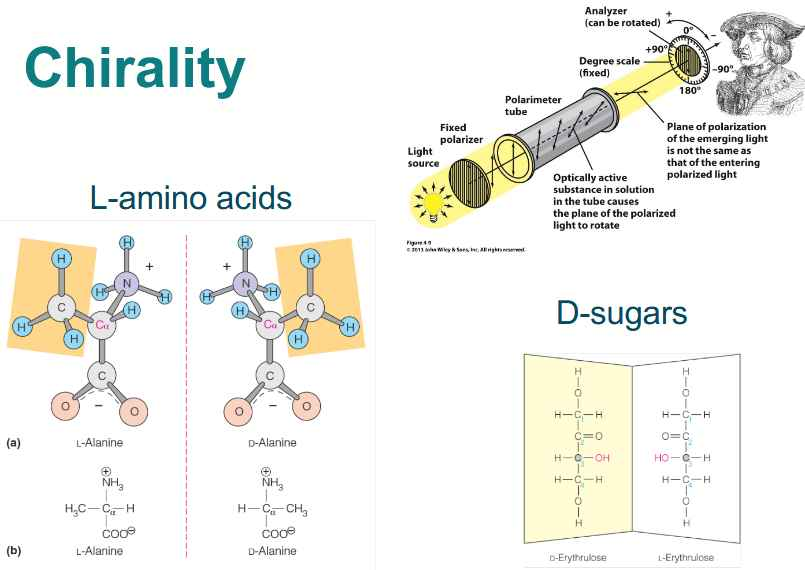
\includegraphics[width=0.8\textwidth]{Chirality}
\end{figure}

\begin{figure}[H]
	\caption[All living organisms use membranes]{All living organisms use membranes to separate themselves from the environment}\label{fig:Membranes}
	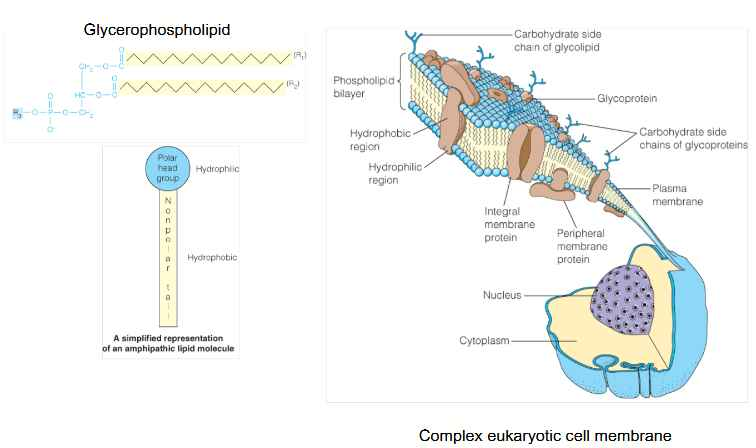
\includegraphics[width=0.8\textwidth]{Membranes}
\end{figure}
\begin{figure}[H]
	\caption[Comparison of similarity allows for the
		construction of a tree]{Comparison of similarity allows for the
		construction of a tree, outlining evolution. Large part of conserved set involved in Central Dogma, and also metabolic.}\label{fig:Phylogeny} 
	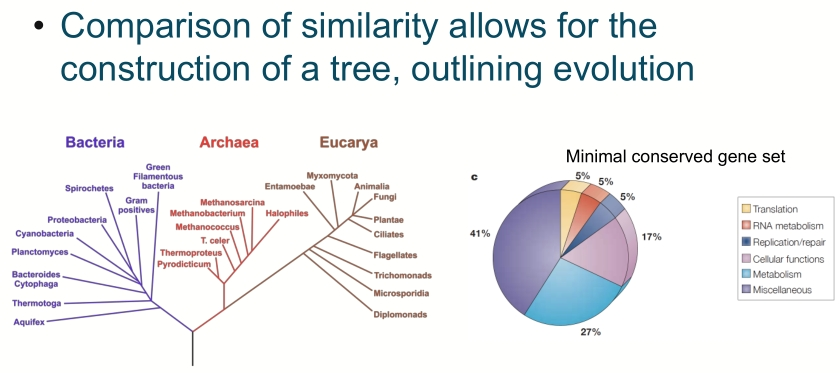
\includegraphics[width=0.9\textwidth]{Phylogeny}
\end{figure}

\begin{figure}[H]
	\caption{Horizontal gene transfer complicates things!}\label{fig:PhylogenyHorizontal} 
	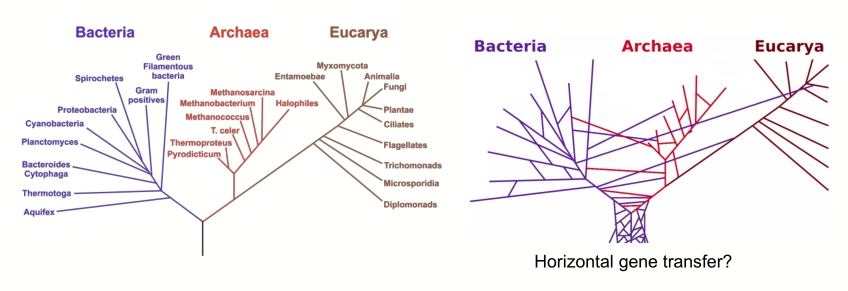
\includegraphics[width=0.9\textwidth]{PhylogenyHorizontal}
\end{figure}



\section{What is Life?}

\subsection[Constraining the Definition of Life]{Constraining the Definition of Life--Sara Imari Walker}

Schrödinger wondered whether we could explain life using physics as currently known.

''... living matter, while not eluding the laws of physics as established up to date, is likely to involve other laws of physics hitherto unknown''--Erwin Schrödinger\cite{schrodinger1944life}.

WE don't really know what life looks like, but we might ask critically what are the examples of life on Earth, and how we can use them to build a unified theory of what life is--a real predictive theory that allows us to understand nit just life on this planet, but also life on other worlds. In physics we have this wonderful hierarchy of theories--Figure \ref{fig:physics:unifications}, but it doesn't have anything to say about complex systems or about us: ''The theory of everything is a theory of everything except of those things that theorize''--David Krakauer.

So the challenge is how can we think about how we can approach an explanatory theory for life, and whether we can draw inspiration from the history of physics. So it is constructive to look at examples of life on earth. Is life really a natural kind? Are some systems more alive than others?

\begin{figure}[H]
	\caption{History of Unifications in Physics}
	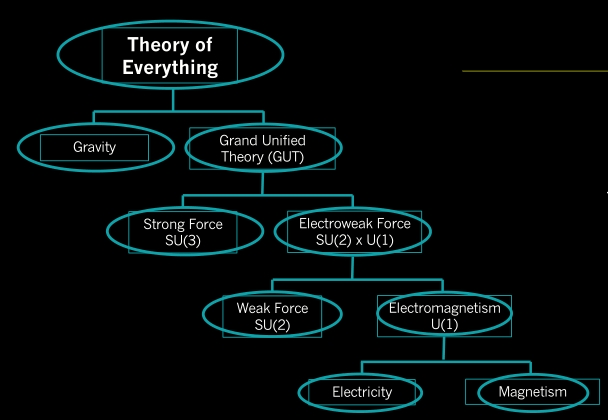
\includegraphics[width=0.9\textwidth]{Unifications}\label{fig:physics:unifications}
\end{figure}


Examples of "Life"
\begin{itemize}
	\item The Cell as a unit of Life--Figure \ref{fig:cell}
	\item Metabolism--Figure \ref{fig:metabolism}
	\item Tardigrade--an extremophile that can live in space--Figure \ref{fig:tardigrade}. Maybe we should think about the widest set of conditions under which life \textit{can} exist.
	\item Two-headed planarian worms--Figure \ref{fig:2headed:planaria}. What is the limit for viable life?\cite{levin2019planarian}
	\item What if we replace RNA/DNA with XNA?
	\item We can consider scales of organization, as with Social Insects--Figure \ref{fig:social:insects}. Is the super-organism, the colony, "alive"? Is life something that emerges in chemistry, but can exist at higher levels?\cite{pratt2015psychology}
	\item Is a City alive--Figure \ref{fig:city}?
	\item Is there life on the scale of the Planet\cite{lovelock1974atmospheric}--Figure \ref{fig:gaia}?
\end{itemize}

\begin{figure}[H]
	\caption{The Cell as a unit of Life}\label{fig:cell}
	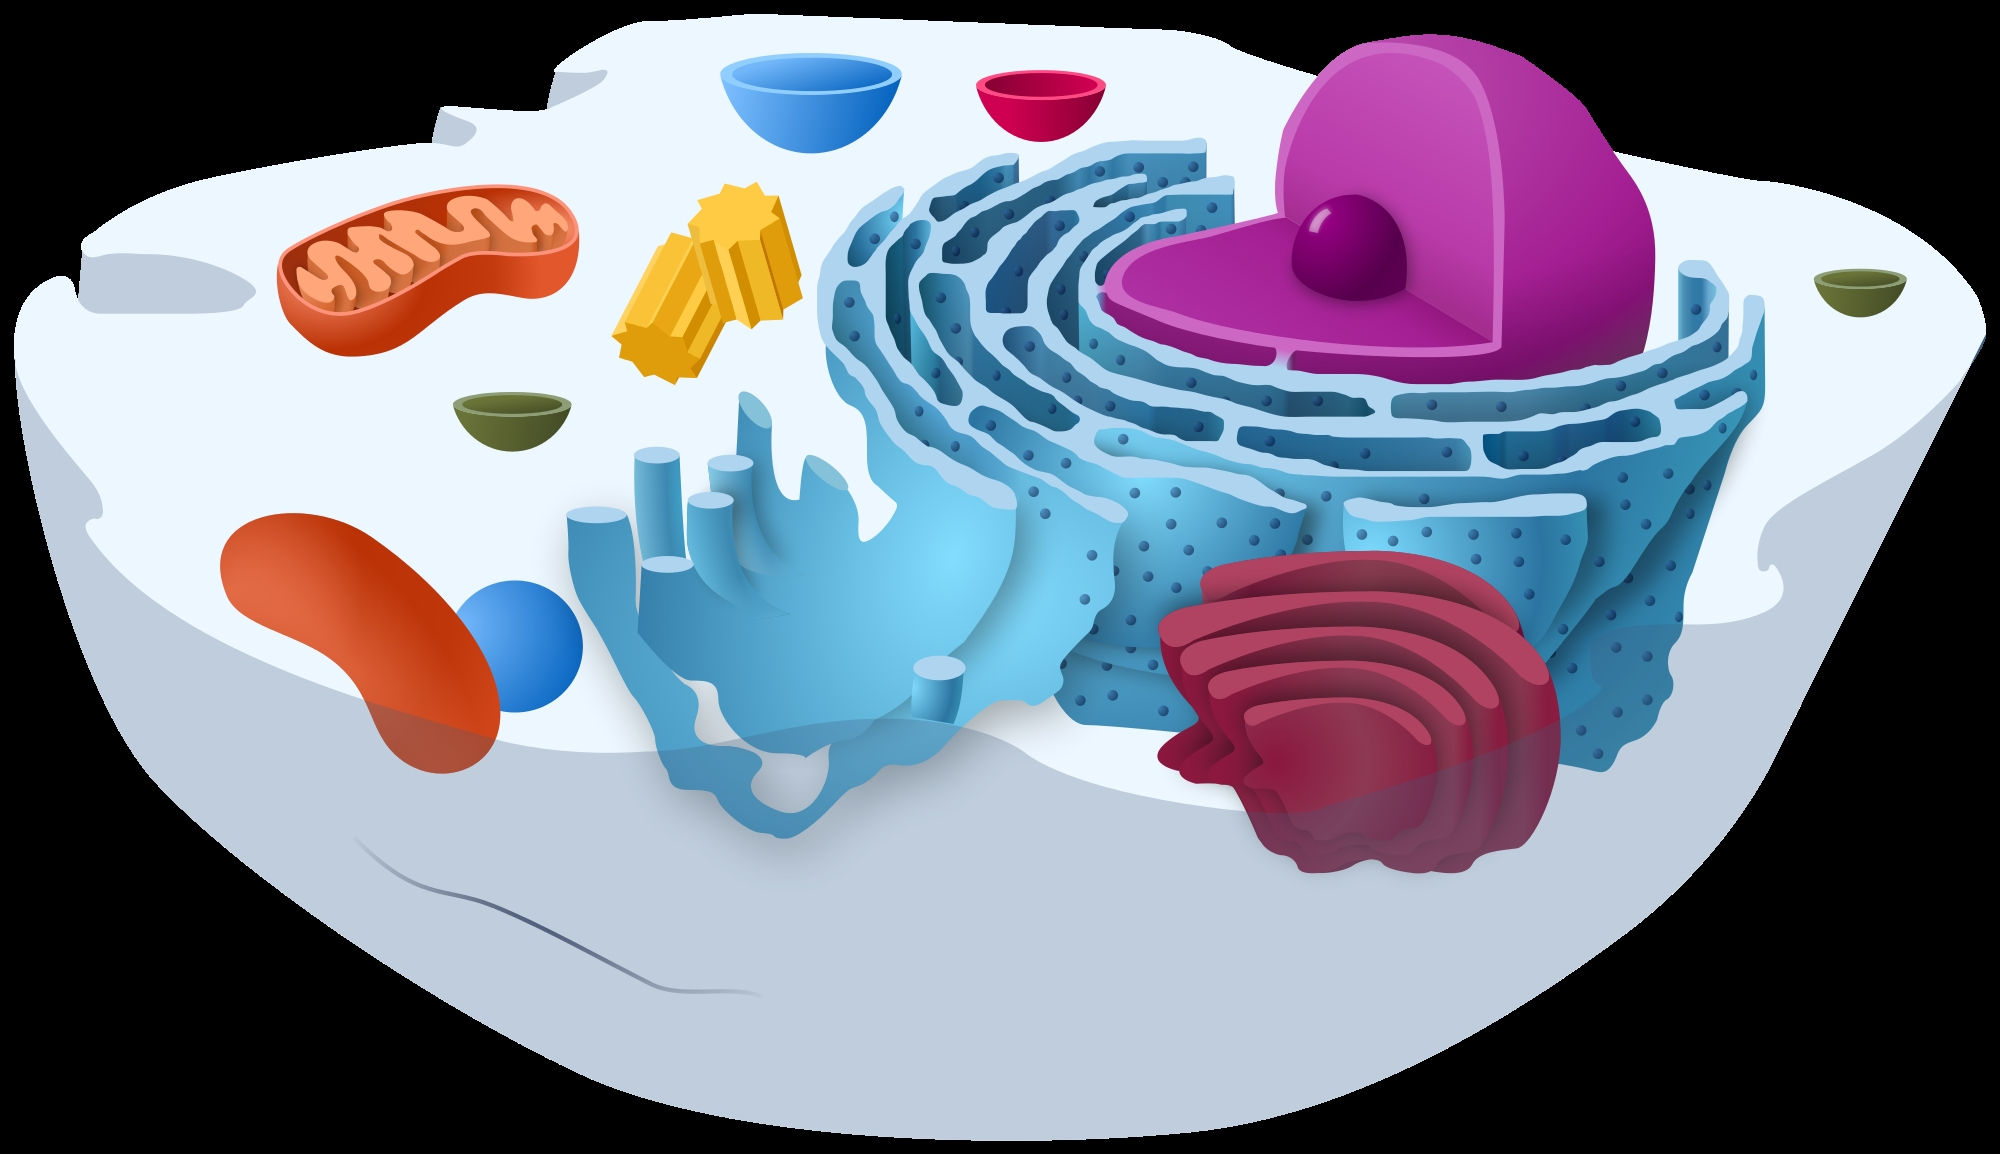
\includegraphics[width=0.9\textwidth]{Cell}
\end{figure}

\begin{figure}[H]
	\caption{Metabolism}\label{fig:metabolism}
	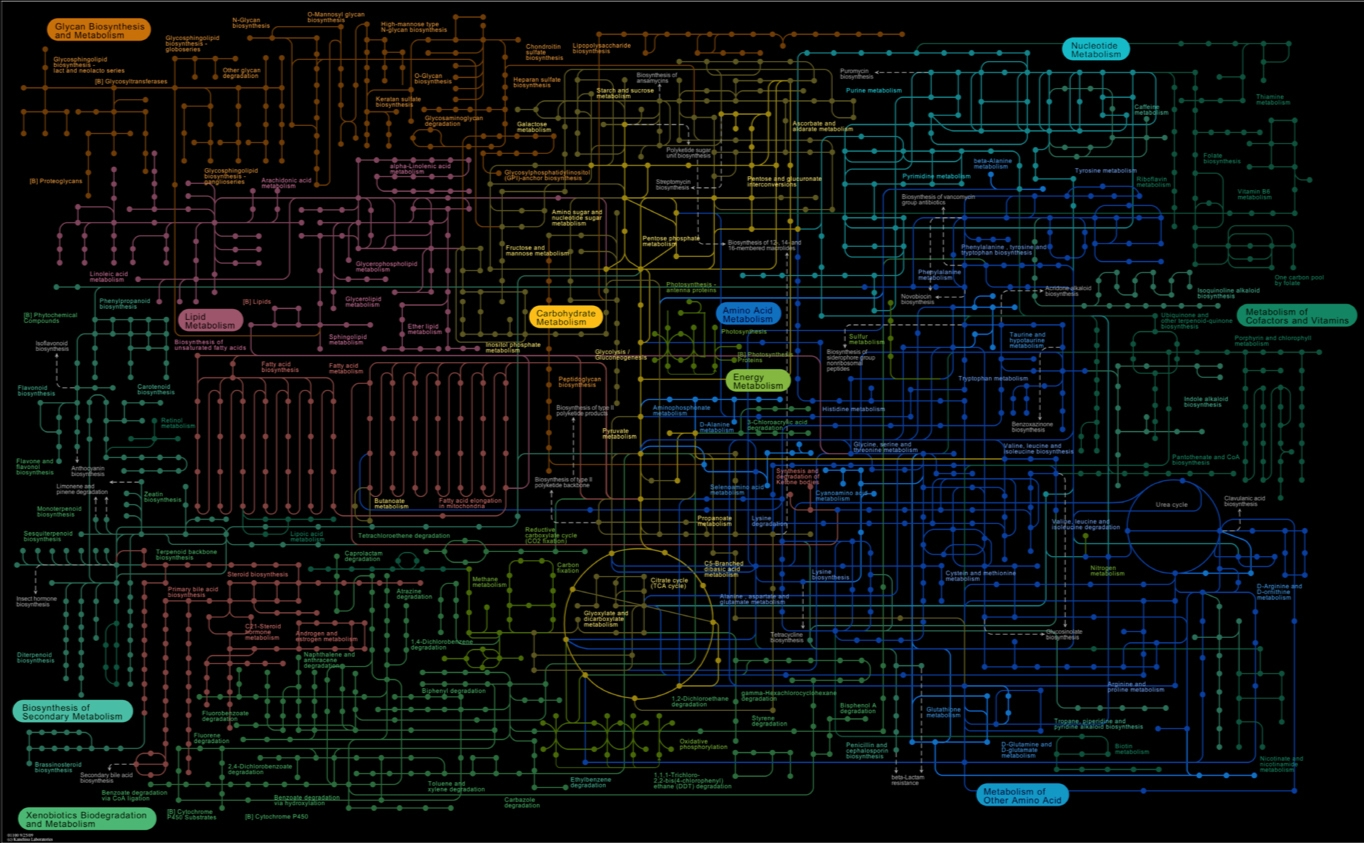
\includegraphics[width=0.9\textwidth]{Metabolism}
\end{figure}

\begin{figure}[H]
	\caption{Tardigrade--an extremophile that can live in space}\label{fig:tardigrade}
	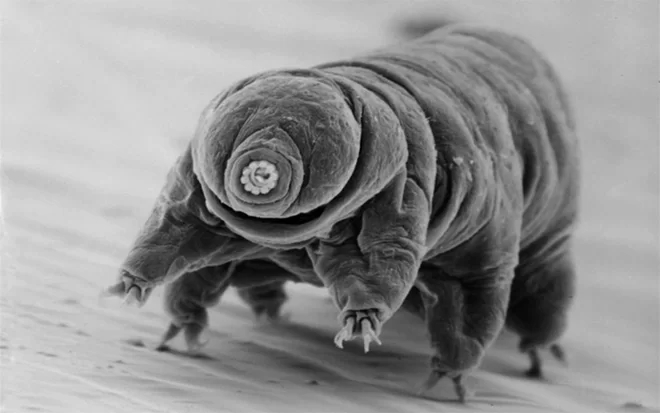
\includegraphics[width=0.9\textwidth]{Tardigrade}
\end{figure}


\begin{figure}[H]
	\caption{Two Headed Planaria}\label{fig:2headed:planaria}
	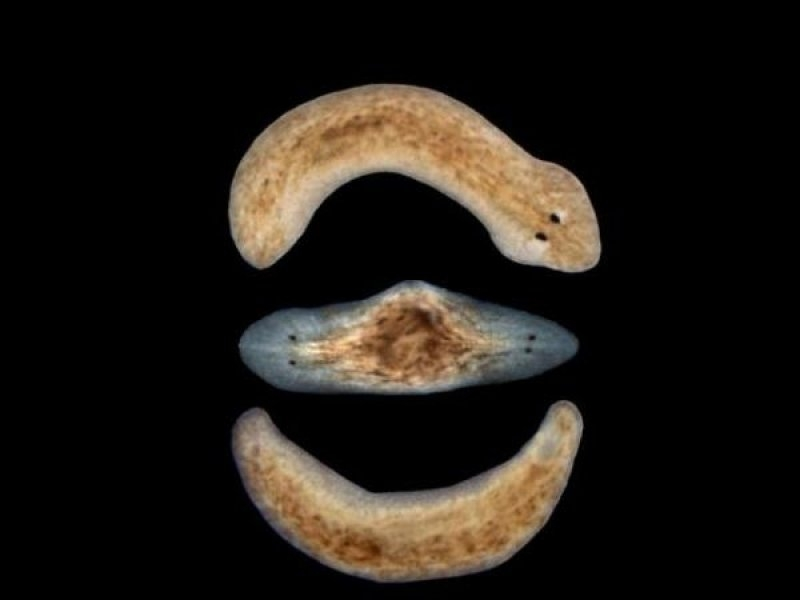
\includegraphics[width=0.9\textwidth]{TwoHeadedPlanaria}
\end{figure}

\begin{figure}[H]
	\caption{Social Insects: is the super-organism "alive"?}\label{fig:social:insects}
	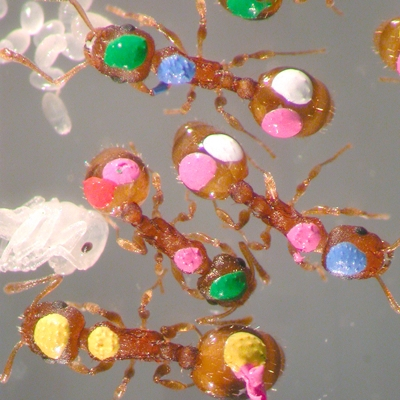
\includegraphics[width=0.9\textwidth]{SocialInsects}
\end{figure}

\begin{figure}[H]
	\caption{City}\label{fig:city}
	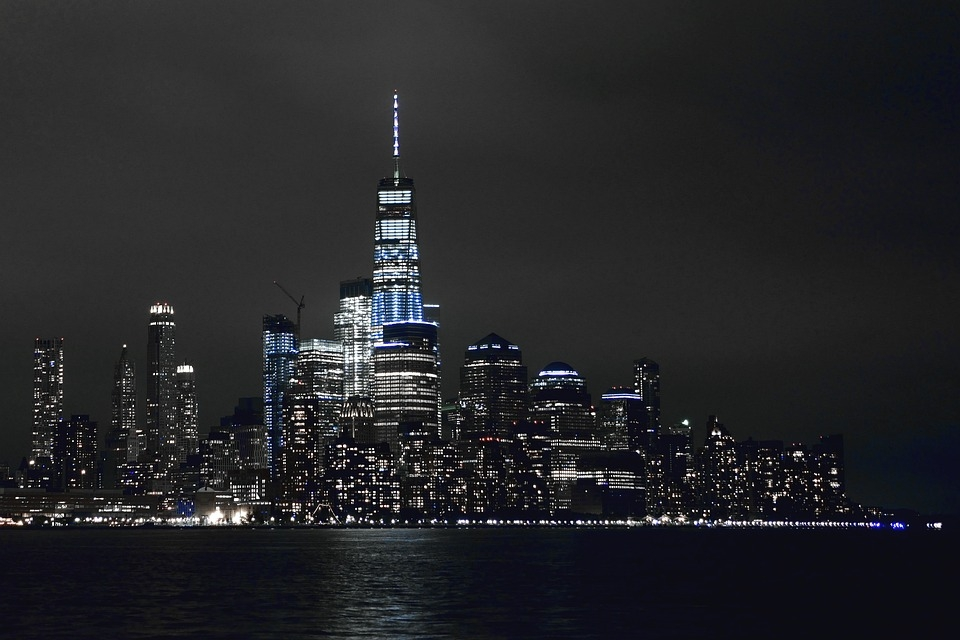
\includegraphics[width=0.9\textwidth]{City}
\end{figure}

\begin{figure}[H]
	\caption{Is there Life on the scale of a Planet?}\label{fig:gaia}
	\begin{subfigure}[b]{0.45\textwidth}
		\caption{Gaia}
		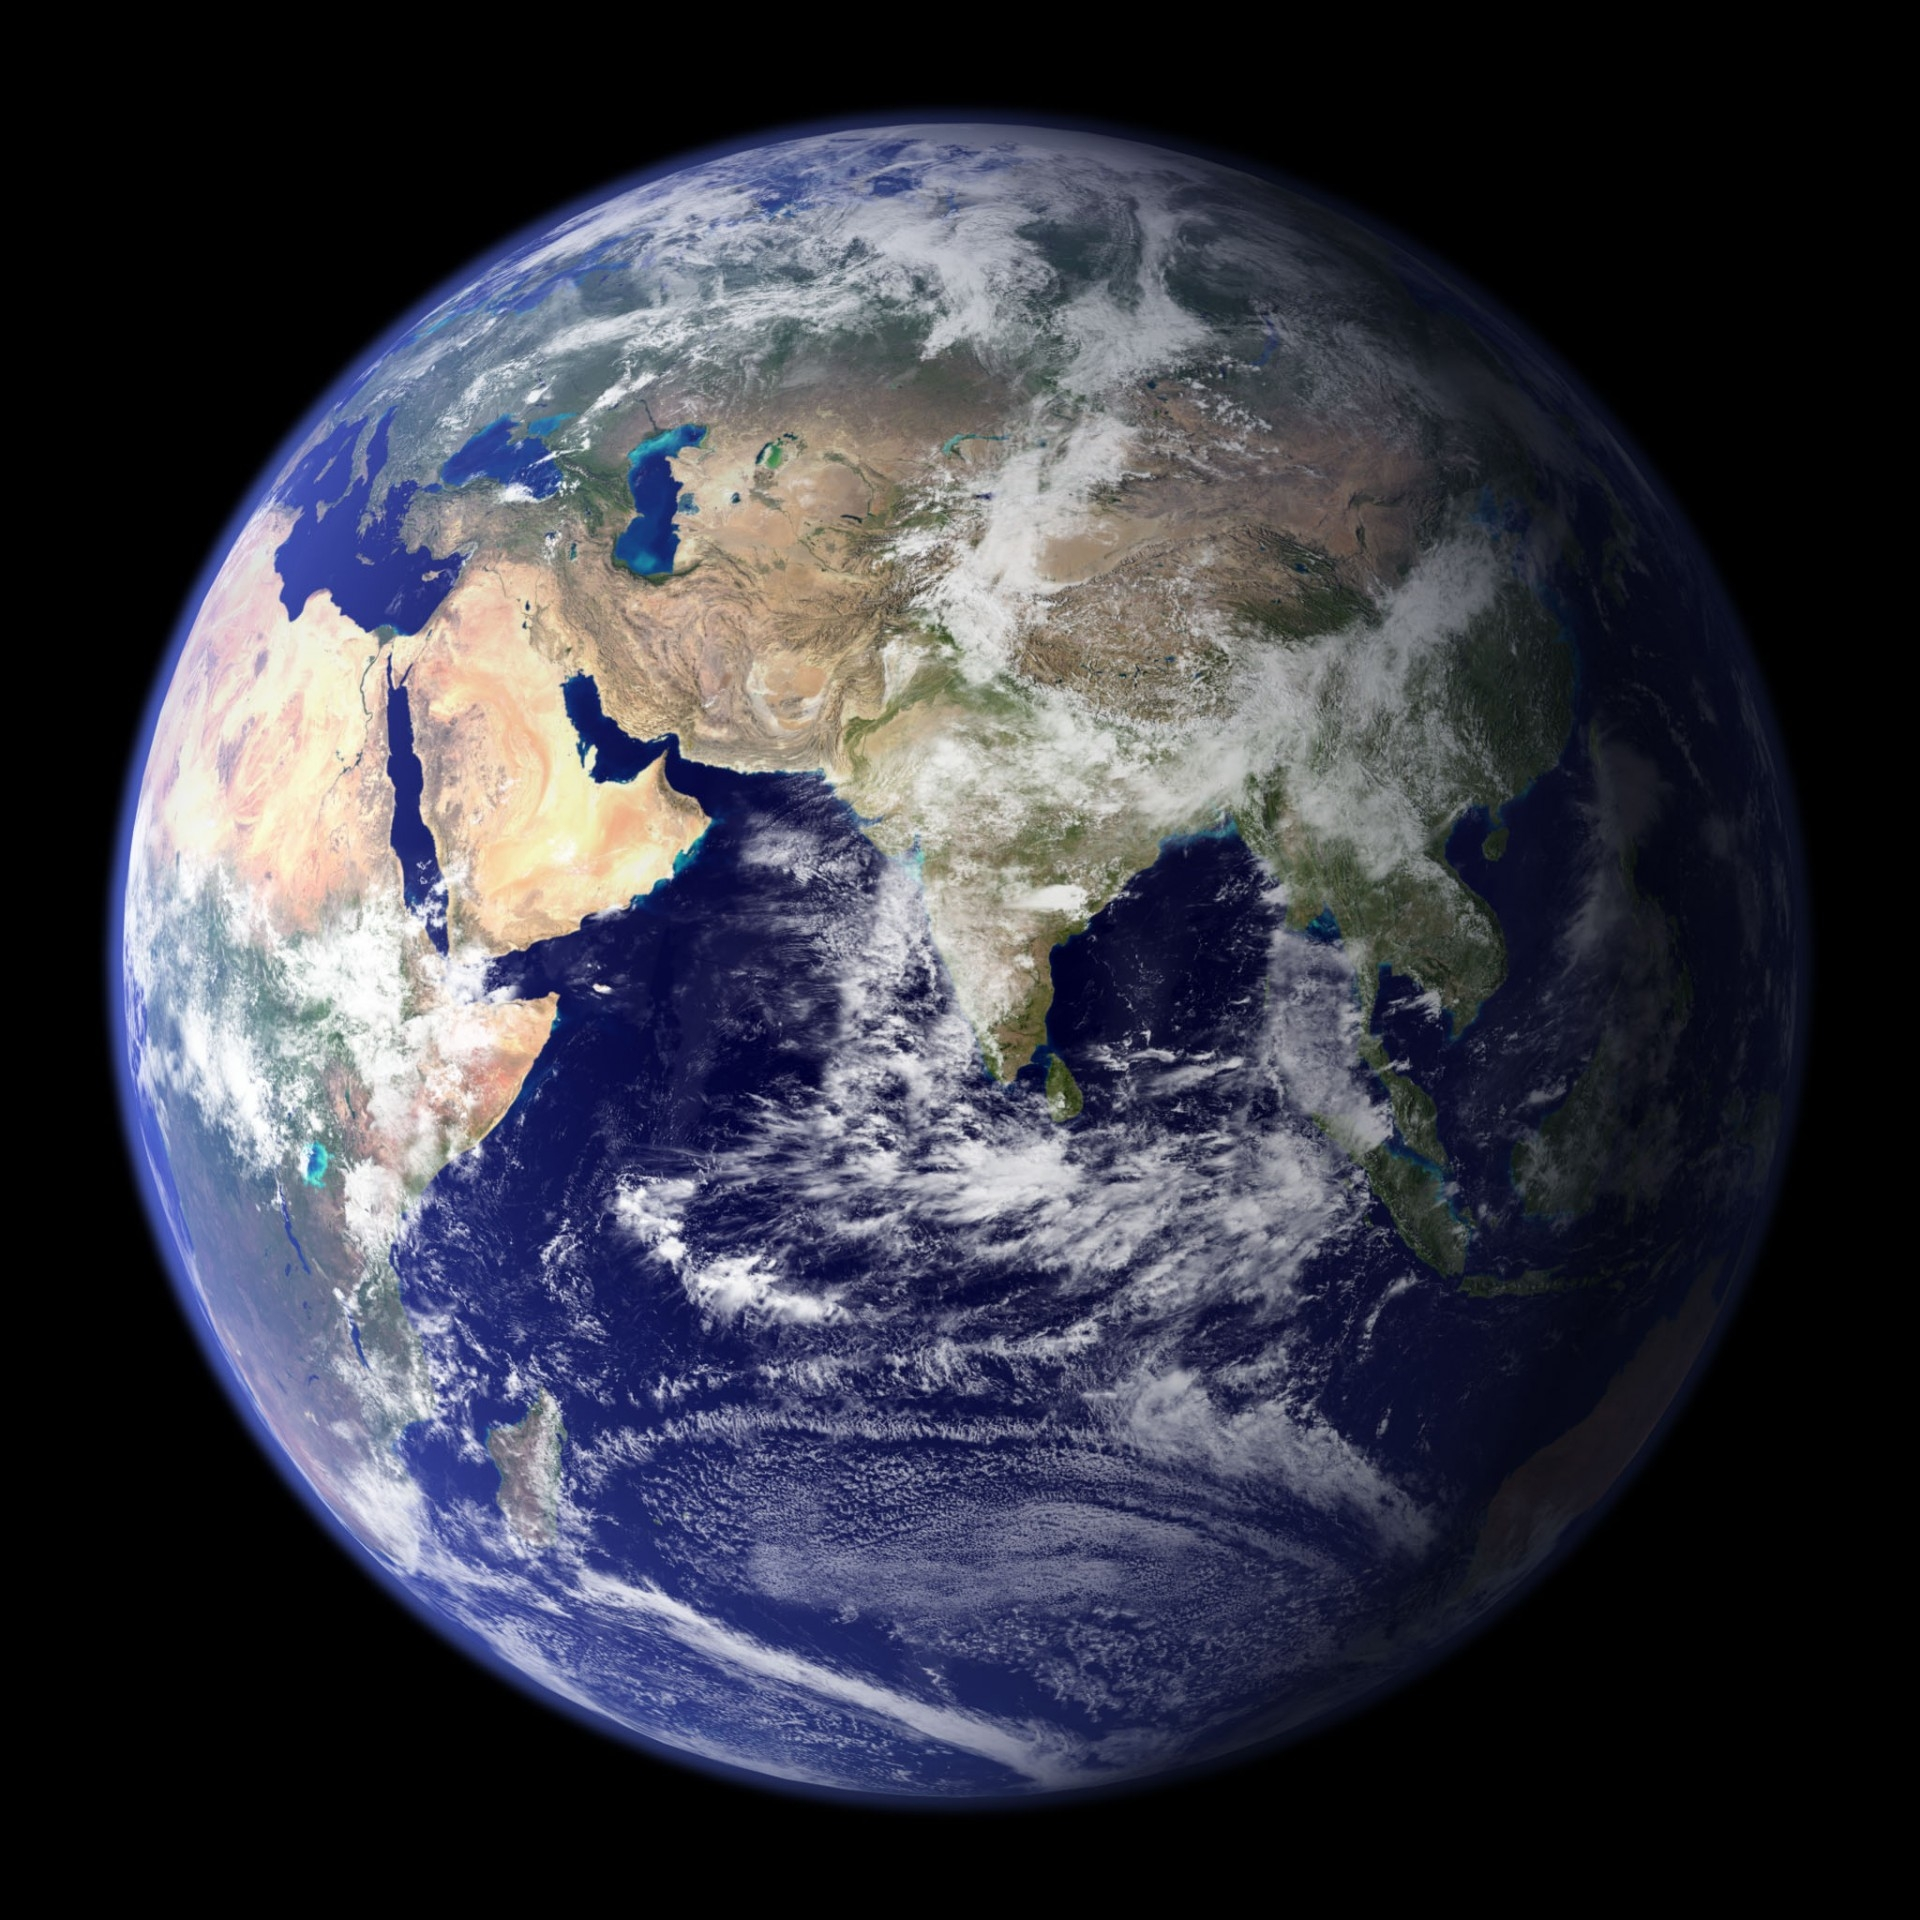
\includegraphics[width=\textwidth]{Globe1}
	\end{subfigure}
	\begin{subfigure}[b]{0.45\textwidth}
		\caption{Network representation of the global inventory of
			enzymatically catalyzed biochemical reactions}
		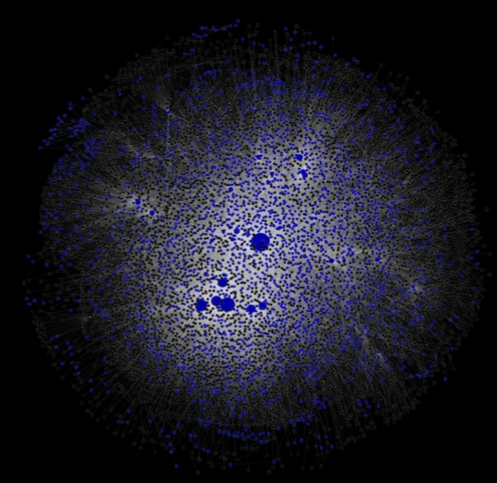
\includegraphics[width=\textwidth]{Globe2}
	\end{subfigure}
\end{figure}


\subsection[Weird Life]{Weird Life--Sarah Maurer}

The material in this section is entirely speculative.

\begin{itemize}
	\item No Cells--diffusion systems. But it is very restrained: have to get the right values for parameters.
	\item Membrane-less Cells? Organization of 	chemical gradients\cite{hollants2011life}\cite{kim2001life}
	\begin{itemize}
		\item Mineral surfaces
		\item Coacervates
		\item Oil droplets
		\item Aerosols
	\end{itemize}
	\item No water? 
	\begin{itemize}
		\item Polar solvents\cite[Chapter 6]{board2007limits}--Figure \ref{fig:no:water}. Water, ammonia, and sulphuric acid can:
		\begin{itemize}
			\item drive formation of carbon-carbon bonds;
			\item hydrogen bond.
		\end{itemize}
		\item Non-polar solvents\cite{cejkova2014dynamics}--Figure \ref{fig:non:polar}.
	\end{itemize}
	\item No liquid?\cite[Chapter 6]{board2007limits}
	\begin{itemize}
		\item Solids
		\begin{itemize}
			\item Ices?
			\item Very slow metabolic rates (longer time scales)
		\end{itemize}
		\item Gases
		\begin{itemize}
			\item Higher temperatures
			\item Less stable large molecules
			\item Much larger (galaxy level?)
		\end{itemize}
	\end{itemize}
\end{itemize}


\begin{figure}[H]
	\caption{No Water? Polar solvents}\label{fig:no:water}
	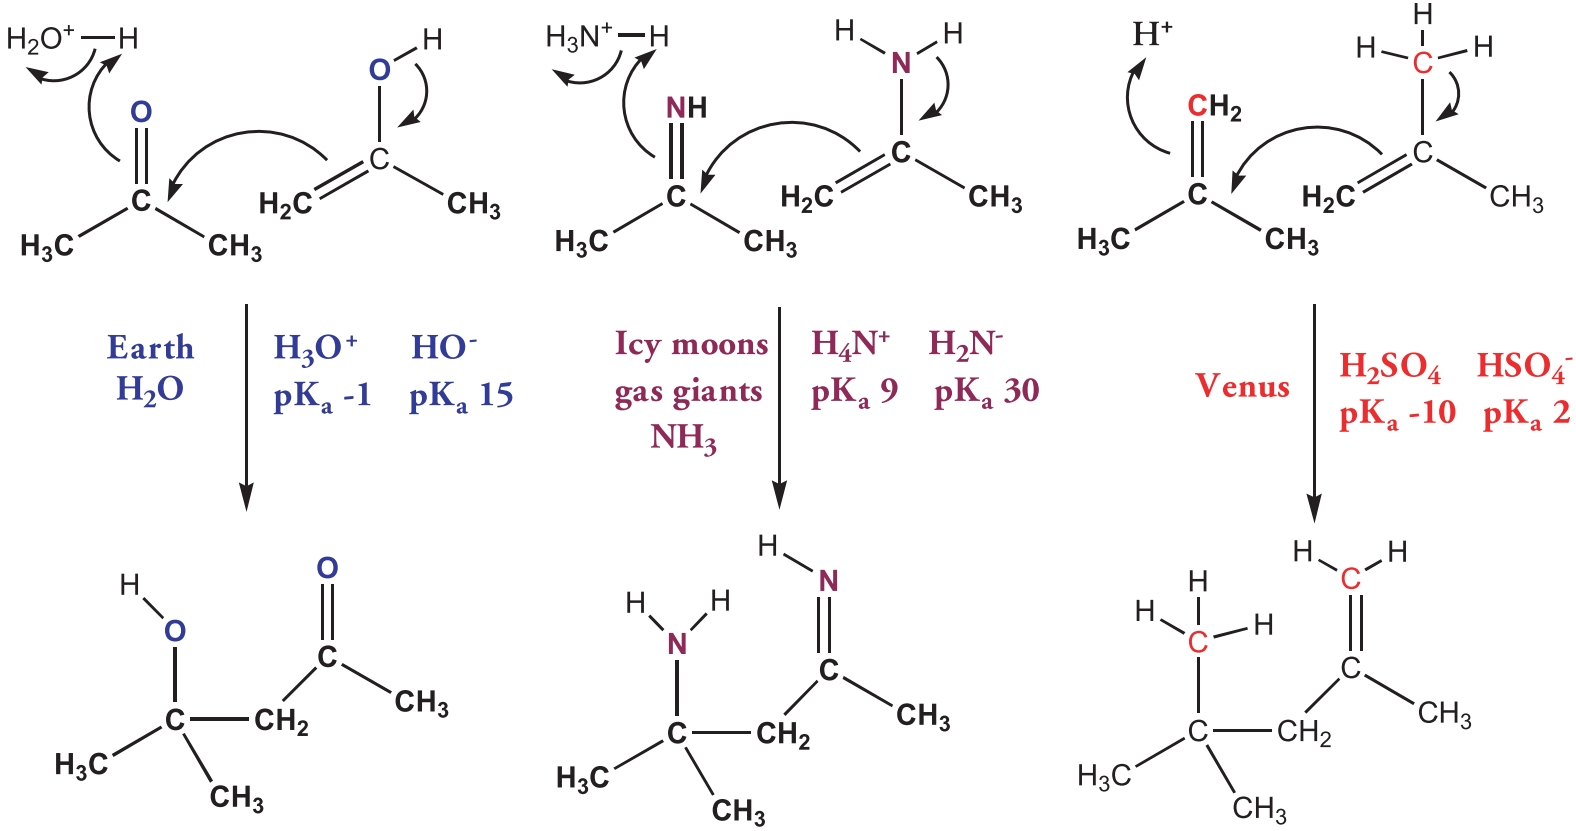
\includegraphics[width=0.9\textwidth]{NoWater}
\end{figure}

\begin{figure}[H]
	\caption{No water? Non-polar solvents}\label{fig:non:polar}
	\begin{subfigure}[t]{0.5\textwidth}
		\caption{Titan--liquid ethane/methane--very cold}
		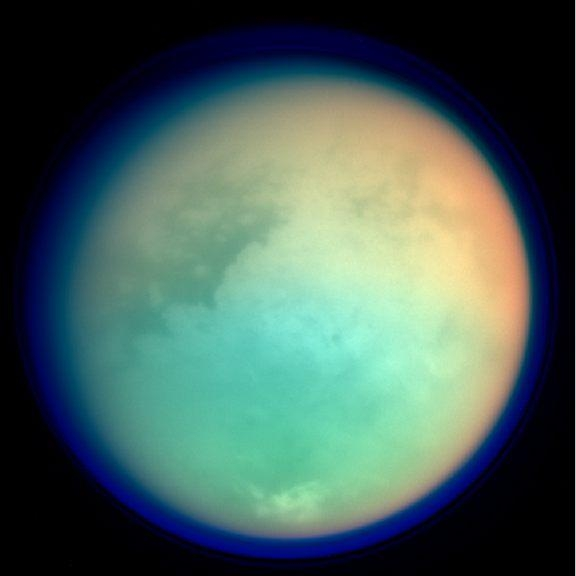
\includegraphics[width=\textwidth]{Titan}
	\end{subfigure}
	\begin{subfigure}[t]{0.5\textwidth}
		\caption{Io--liquid sulfur--Hotter than Earth}
		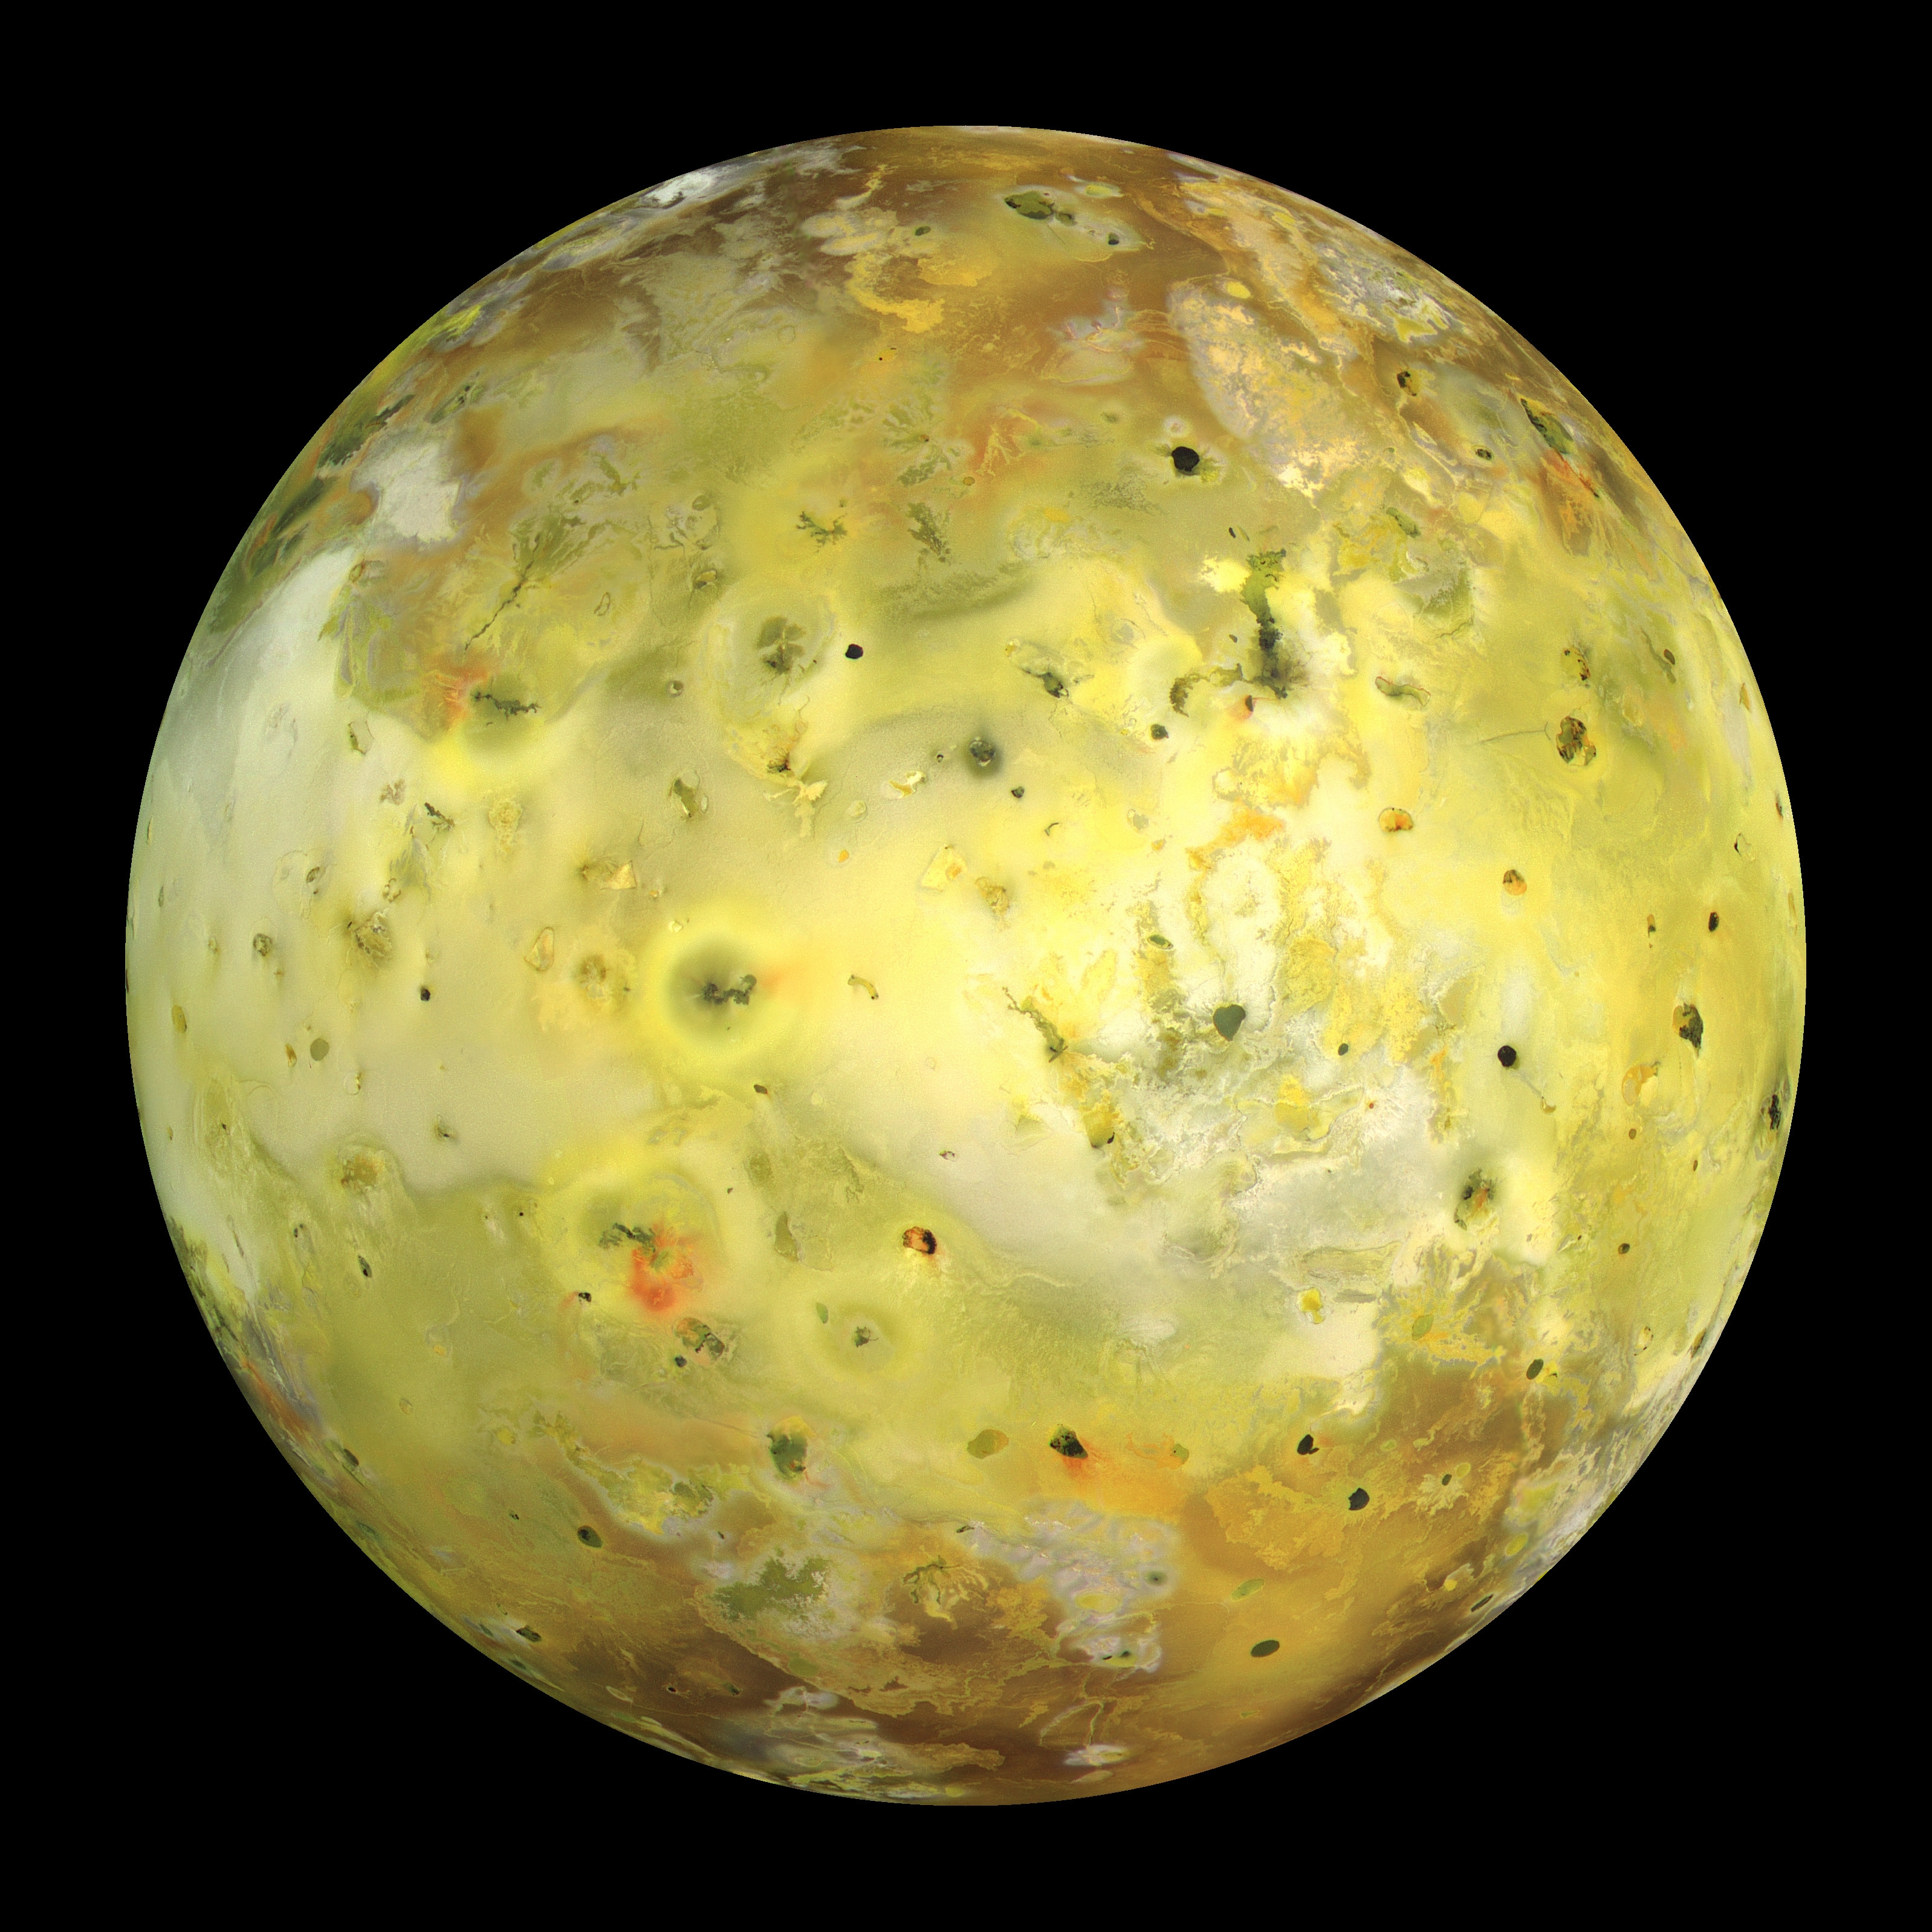
\includegraphics[width=\textwidth]{Io}
	\end{subfigure}
\end{figure}

Open Questions

\begin{itemize}
	\item What other substrates could life exist in?
	\item Would we recognize it?
\end{itemize}


\section[Introduction]{Introduction--Chris Kempes}

We will take a closer look at the detailed chemistry thought to be important to the origin of life. We will discuss
\begin{itemize}
	\item likely chemistry of the early Earth,
	\item chemistry that may be  fundamental to the origin of life,
	\item what chemistry we know is essential for biochemistry of modern life,
	\item processes that can occur in chemical dynamics, 
	\item types of extreme life that occurs today in a variety of environments.
\end{itemize}


\section{What Did Early Earth Look Like?}

\subsection[Geochemical Landscape]{Geochemical Landscape--Sarah Mauer}

We are going to look at what earth looked like between 4.2 and 3.8 billion years ago, and how that might relate to the origins of life. The first thing to know is what the Geochemical landscape looked like--Figure \ref{fig:GeochemicalLandscape}.

\begin{itemize}
	\item  Definitely an ocean that was warmer than today's oceans, probably saltier.\footnote{''While this is not my exact field of study, I am told that water-rock-atmosphere equilibriums operate at orders of magnitude faster time scales than planetary evolution. So the ocean “quickly” came to equilibrium with early oceans (maybe a million years or less), then as new rock was exposed, and the atmosphere changed, the equilibrium shifted. The composition may have been different, with more reduced metals for example, but sodium chloride is the most abundant ionic compound and likely always has been.''--Sarah Maurer}\cite{knauth1998salinity} 
	\item Landmasses from volcanic activity, and, maybe, plate tectonics.
	\item On continents, lakes and ponds from precipitation.  Maybe temporary streams from precipitation.
	\item Surfaces composed of minerals, which were good for catalysis and energy production. Today covered with life.
\end{itemize}

\begin{figure}[H]
	\caption[Geochemical Landscape]{Geochemical Landscape after \cite{kitadai2018origins}} \label{fig:GeochemicalLandscape}
	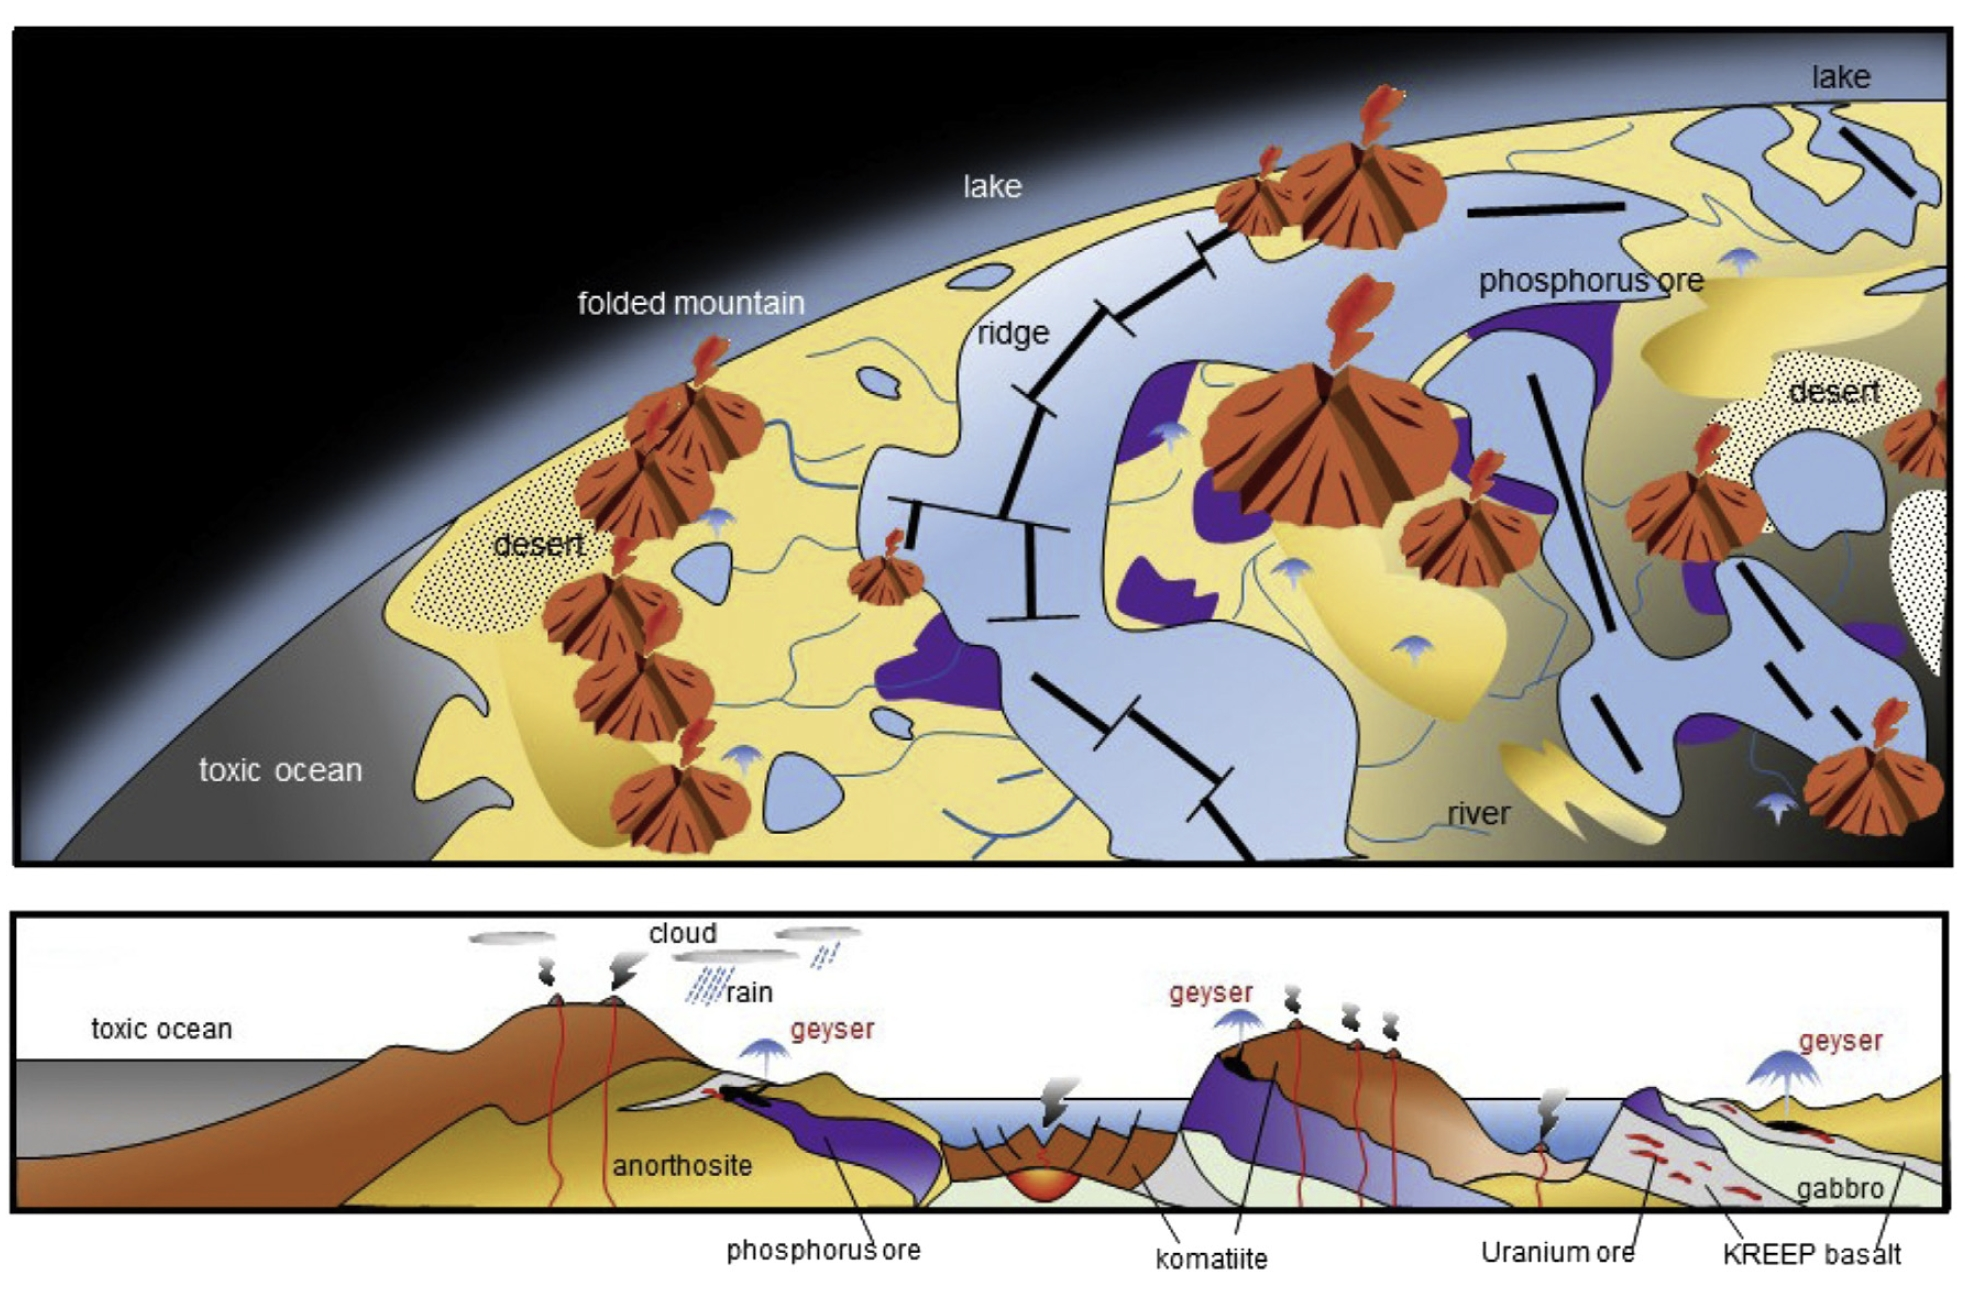
\includegraphics[width=0.9\textwidth]{GeochemicalLandscape}
\end{figure}


\subsubsection{Mixing processes between chemical reactors}

The different chemical reactions that were occurring on early Earth would have been mixed through a variety of different processes, similar to today, so there were likely tides, mixing between the ocean and the inland lakes through evaporation, aerosols, volcanic plumes, carrying molecules to location where different chemistry could occur. All this mixing would lead to a unique chemical library through a variety of different reactions--Figure \ref{fig:MixingProcesses}.

\begin{figure}[H]
	\caption[Mixing processes between chemical reactors]{Mixing processes between chemical reactors \cite{stueken2013did}}\label{fig:MixingProcesses}
	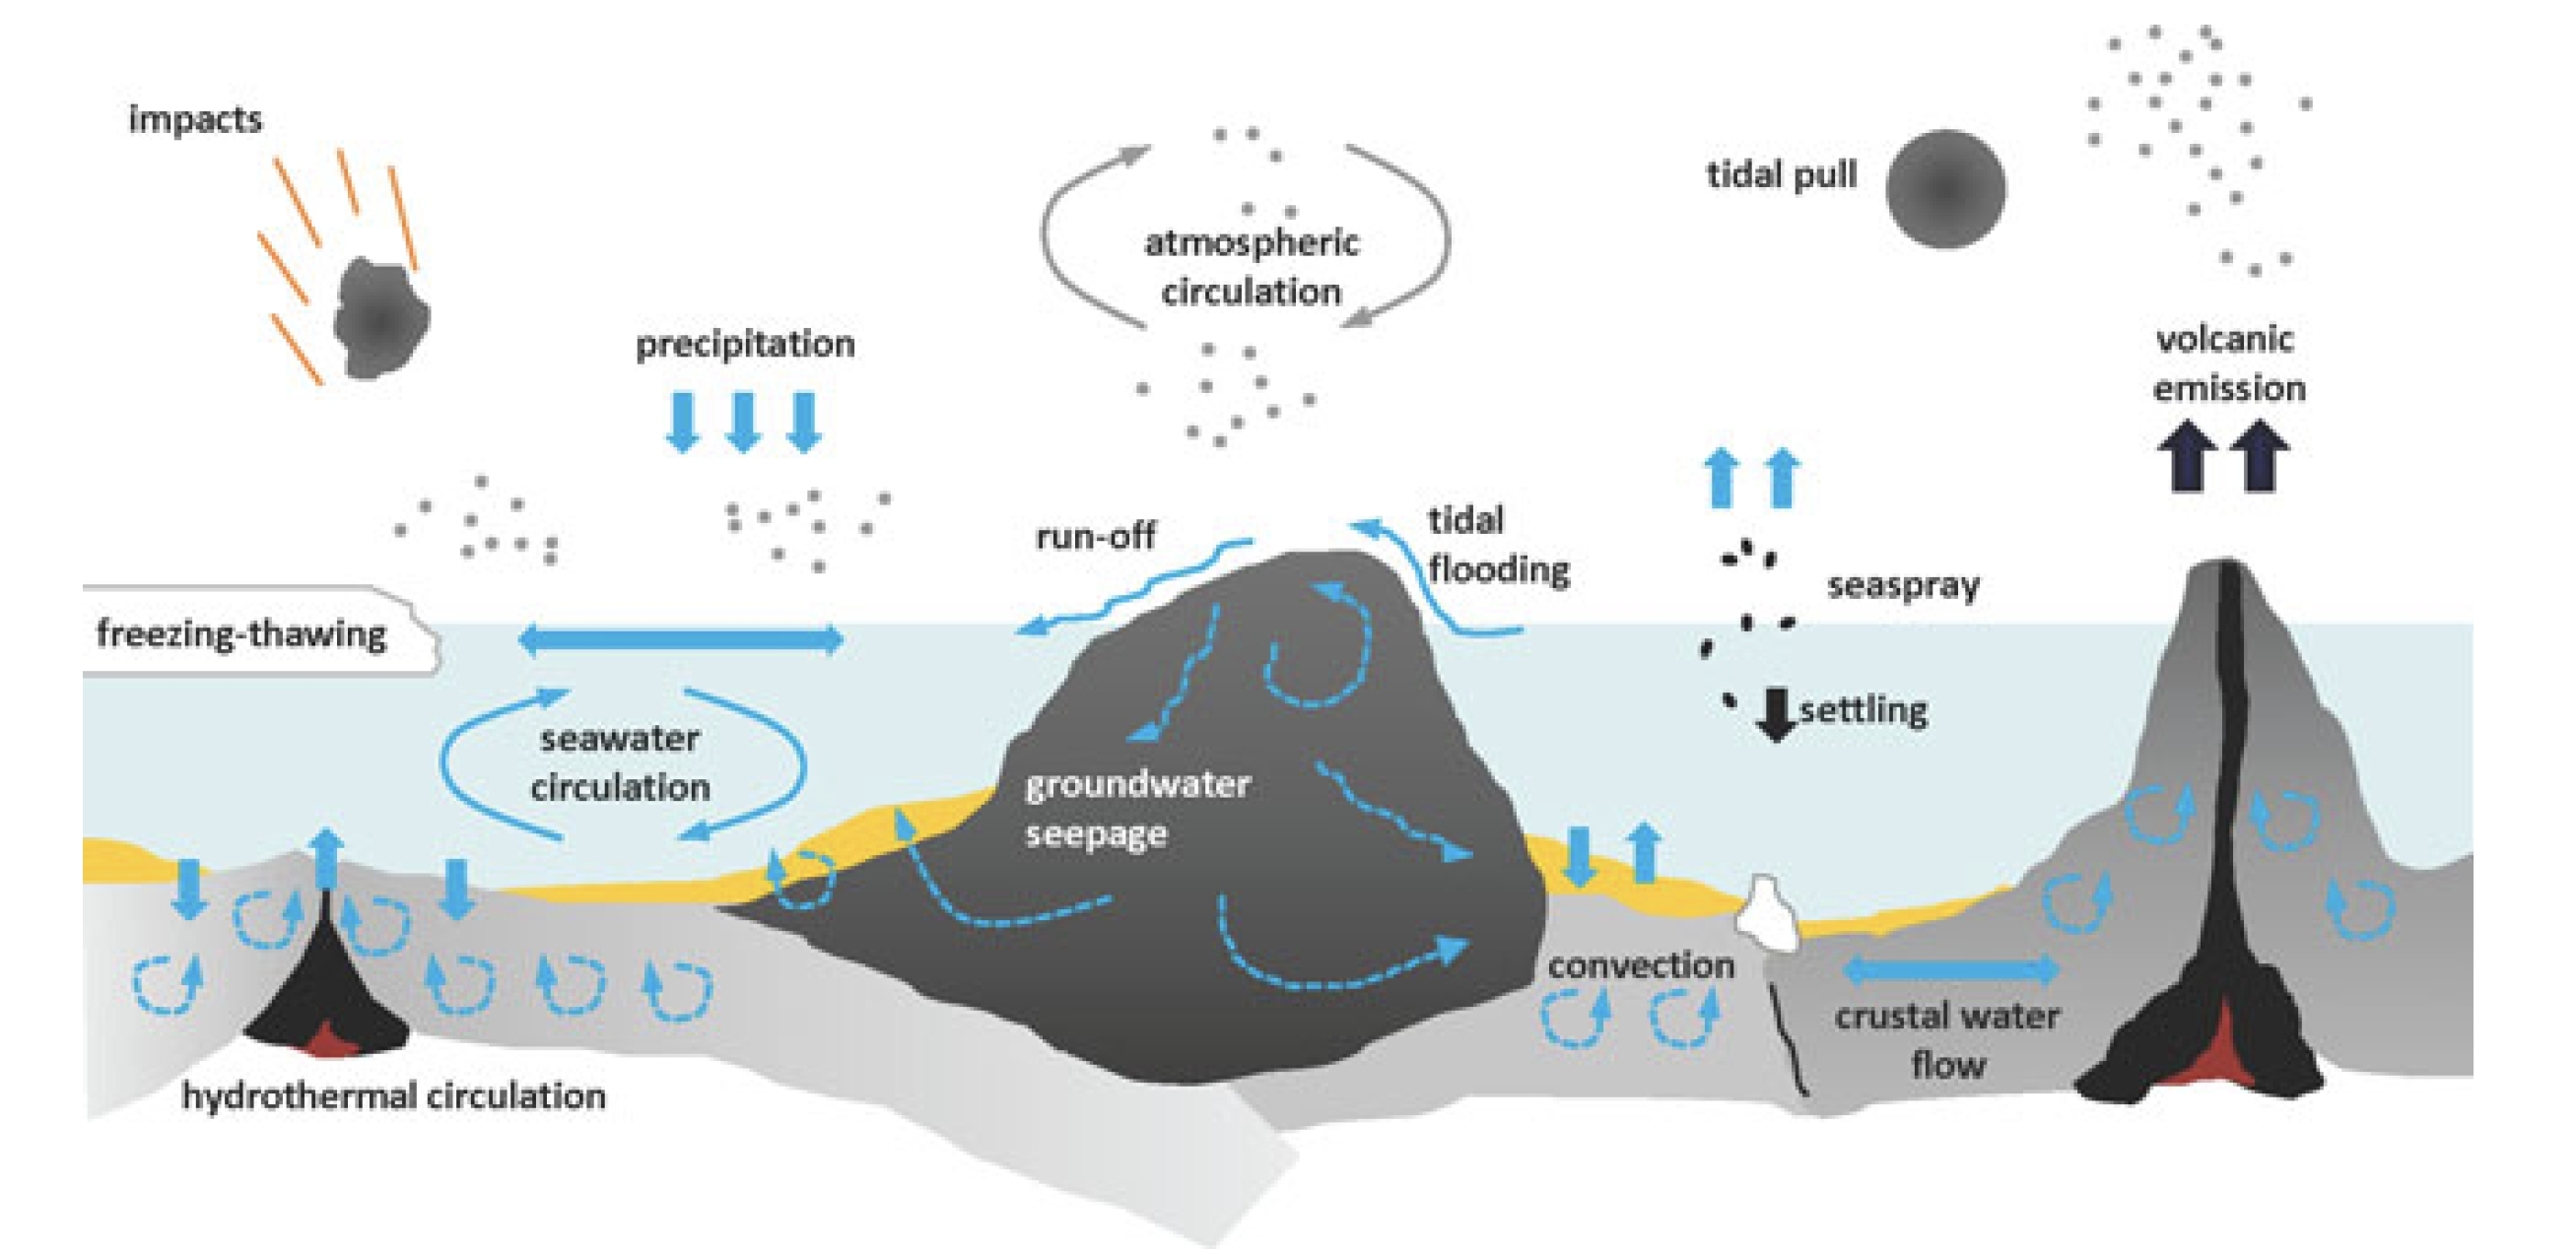
\includegraphics[width=0.8\textwidth]{MixingProcesses}
\end{figure}



\subsubsection{Geothermal systems}
\begin{figure}[H]
	\caption[Geothermal systems]{Geothermal systems \cite{damer2016field}}
	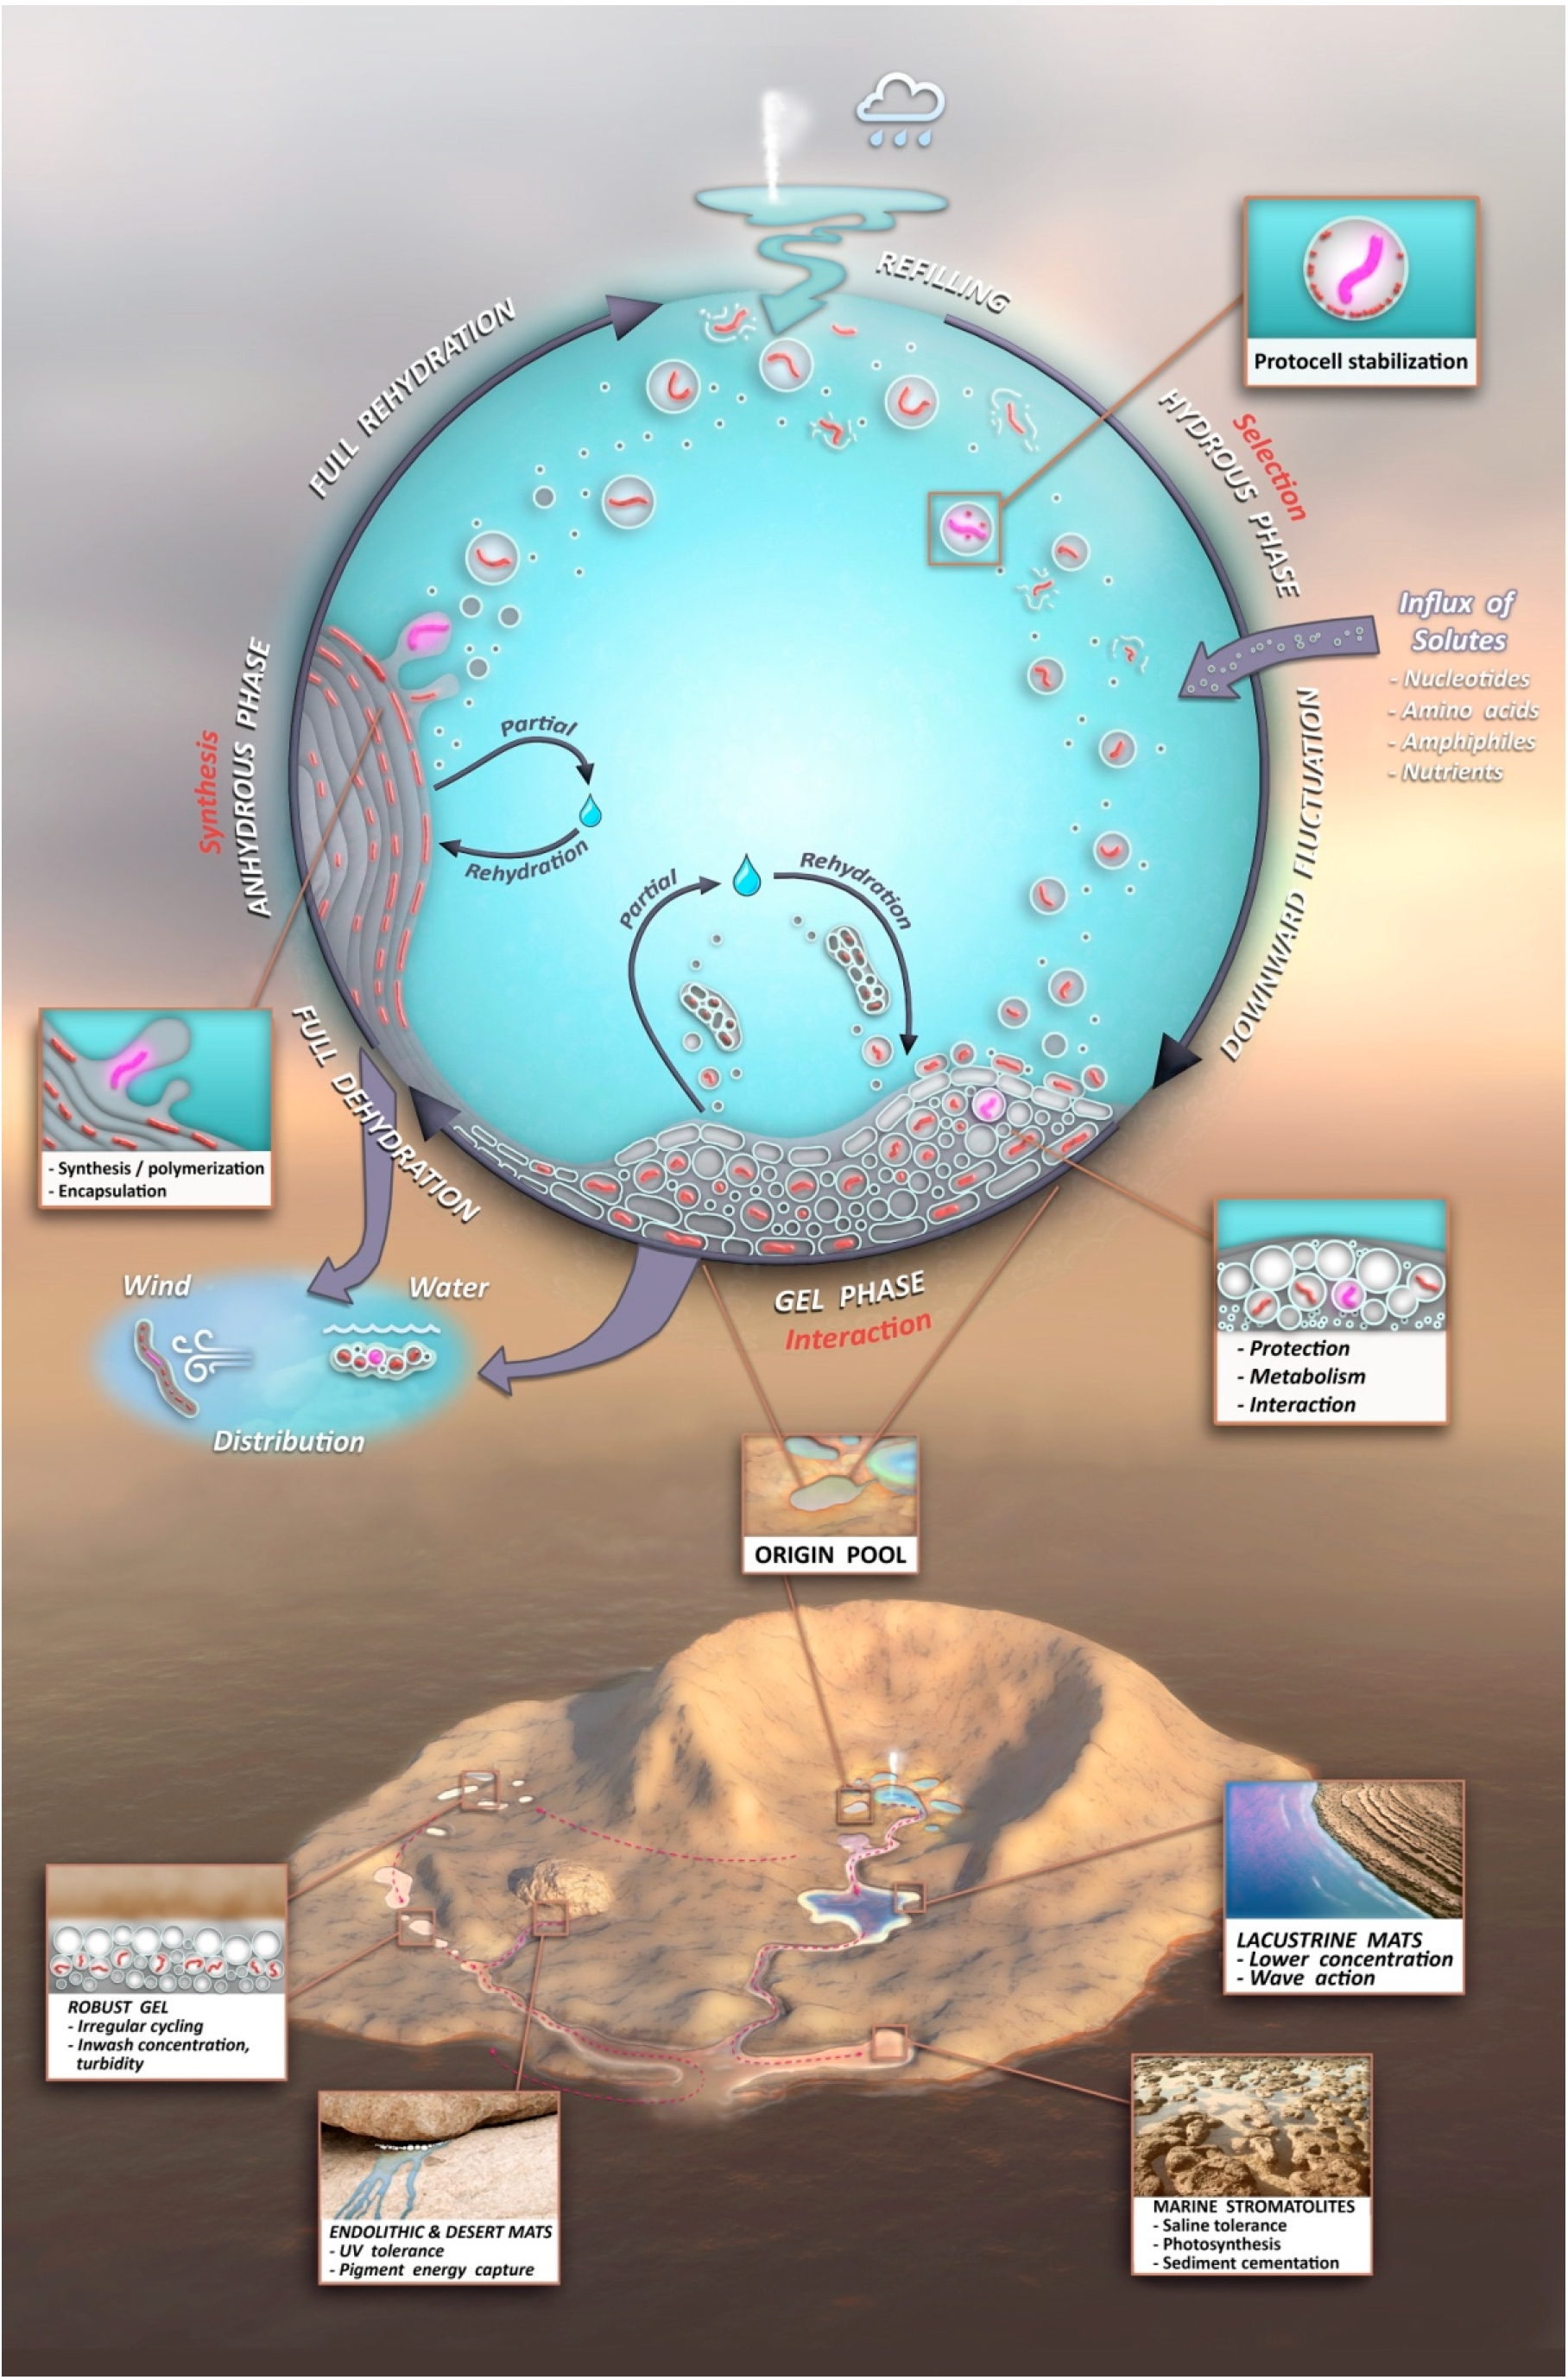
\includegraphics[width=0.9\textwidth]{GeothermalSystems}
\end{figure}

\begin{itemize}
	\item Provide high temperature, high pressure, reduced	reaction products
	\item Fresh water from 	precipitation
	\item Diversity of mineral	surfaces for ”nutrients” and catalysis
\end{itemize}

\subsubsection{Energy Sources}

See \cite{kitadai2018origins}, \cite{stueken2013did}, \cite{damer2016field}, \cite{miller1959organic}, \cite{ehrenfreund2002astrophysical},\cite{dalai2016incubating}, and \cite{chyba1997comets}.

\begin{itemize}
	\item Chemical Energy
	\begin{itemize}
		\item Reducing gases
		\item Radiation
		\item Minerals
	\end{itemize}
	\item Other Energy Sources
	\begin{itemize}
		\item Volcanic lightning
		\item UV-light
		\item High temperature
		\item Pressure
		\item Impacts
	\end{itemize}
\end{itemize}
Figure \ref{fig:MillerUrey} depicts the Miller Urey experiment. It now seems likely that there was no methane in the atmosphere of the early Earth, but but we could use CO2 to derive a different mixture.

\begin{figure}[H]
	\caption[Miller Urey Experiment]{Miller Urey Experiment\cite{miller1959organic}}\label{fig:MillerUrey}
	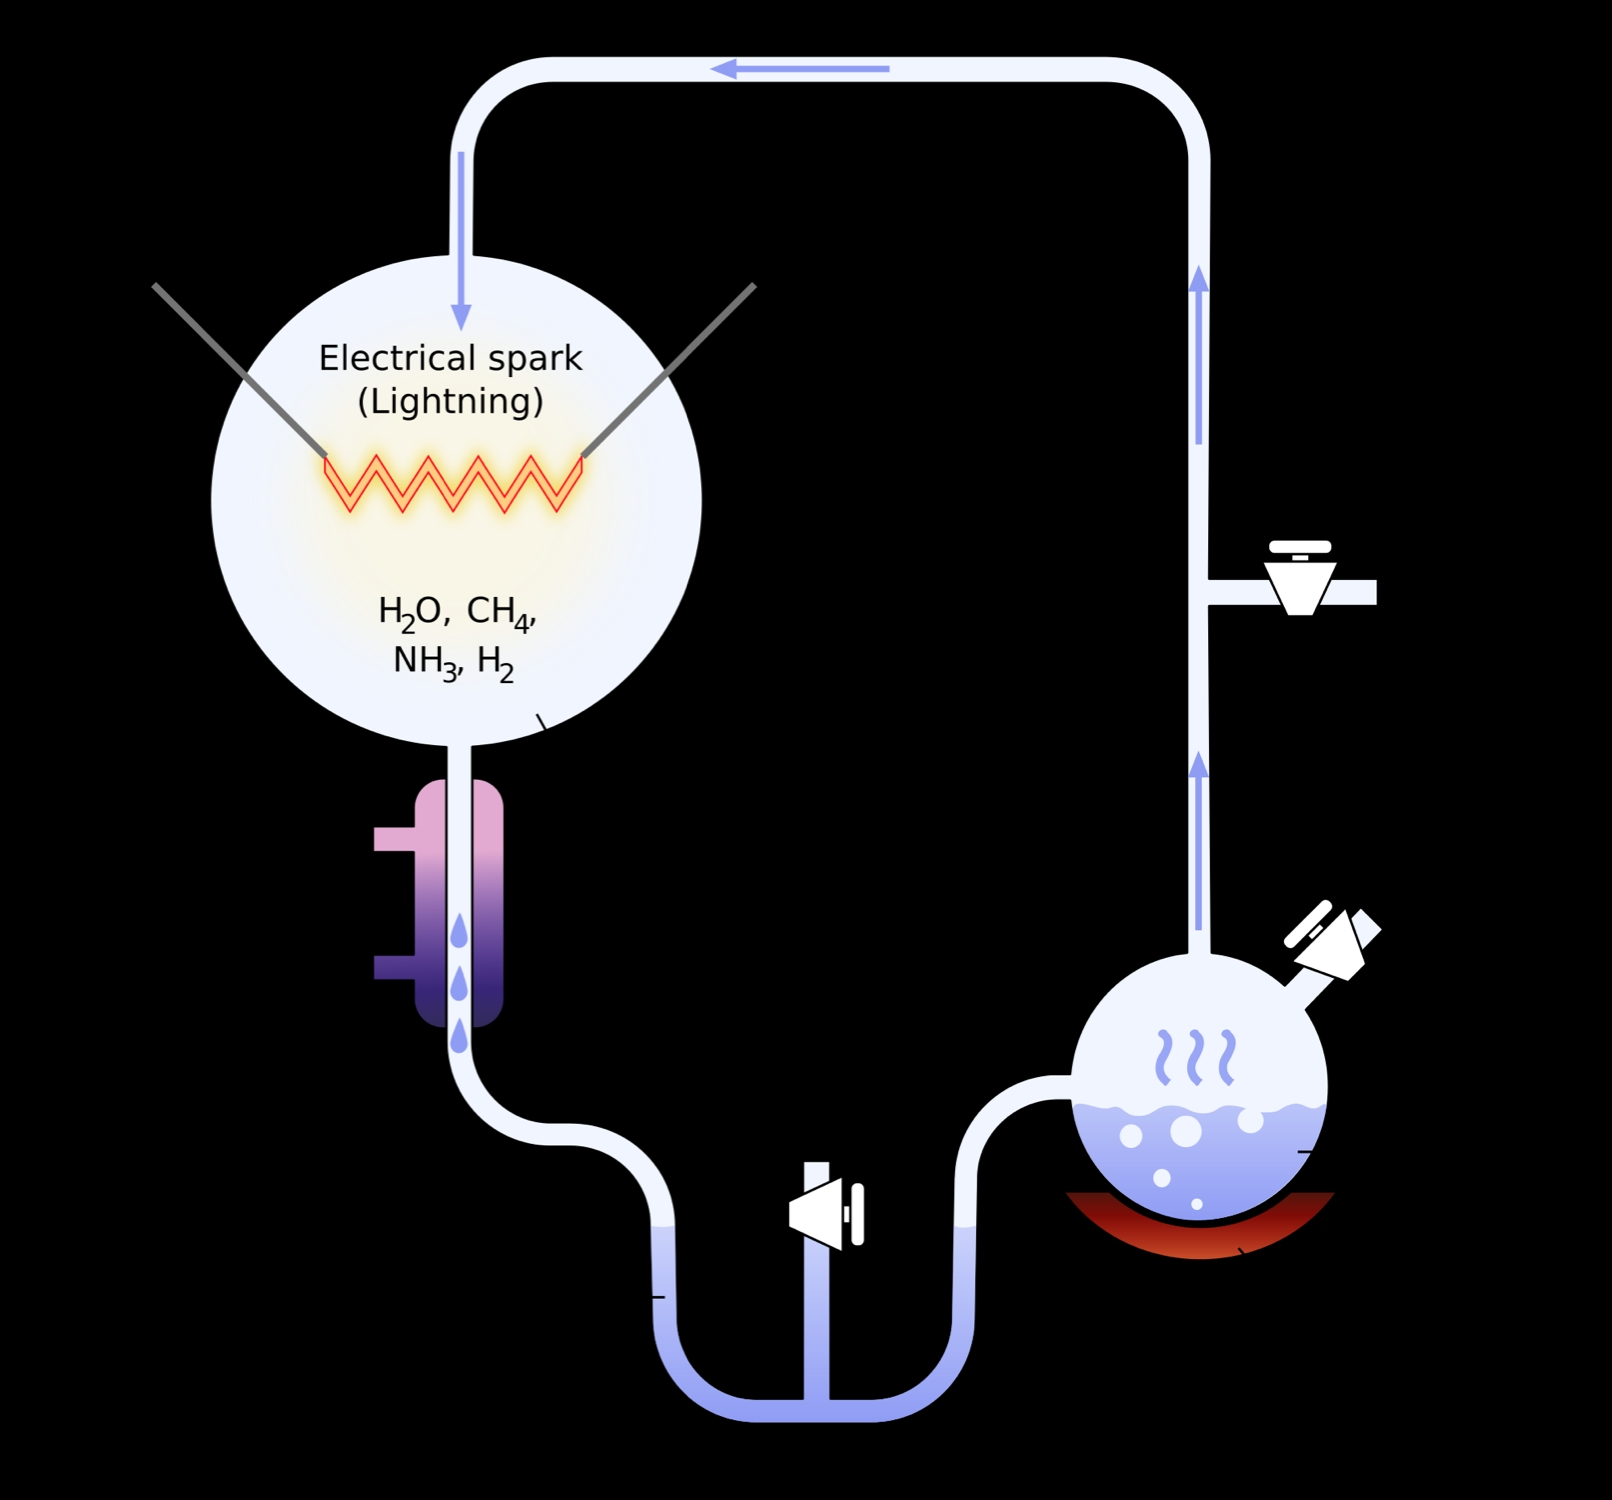
\includegraphics[width=0.45\textwidth]{MillerUrey1}
	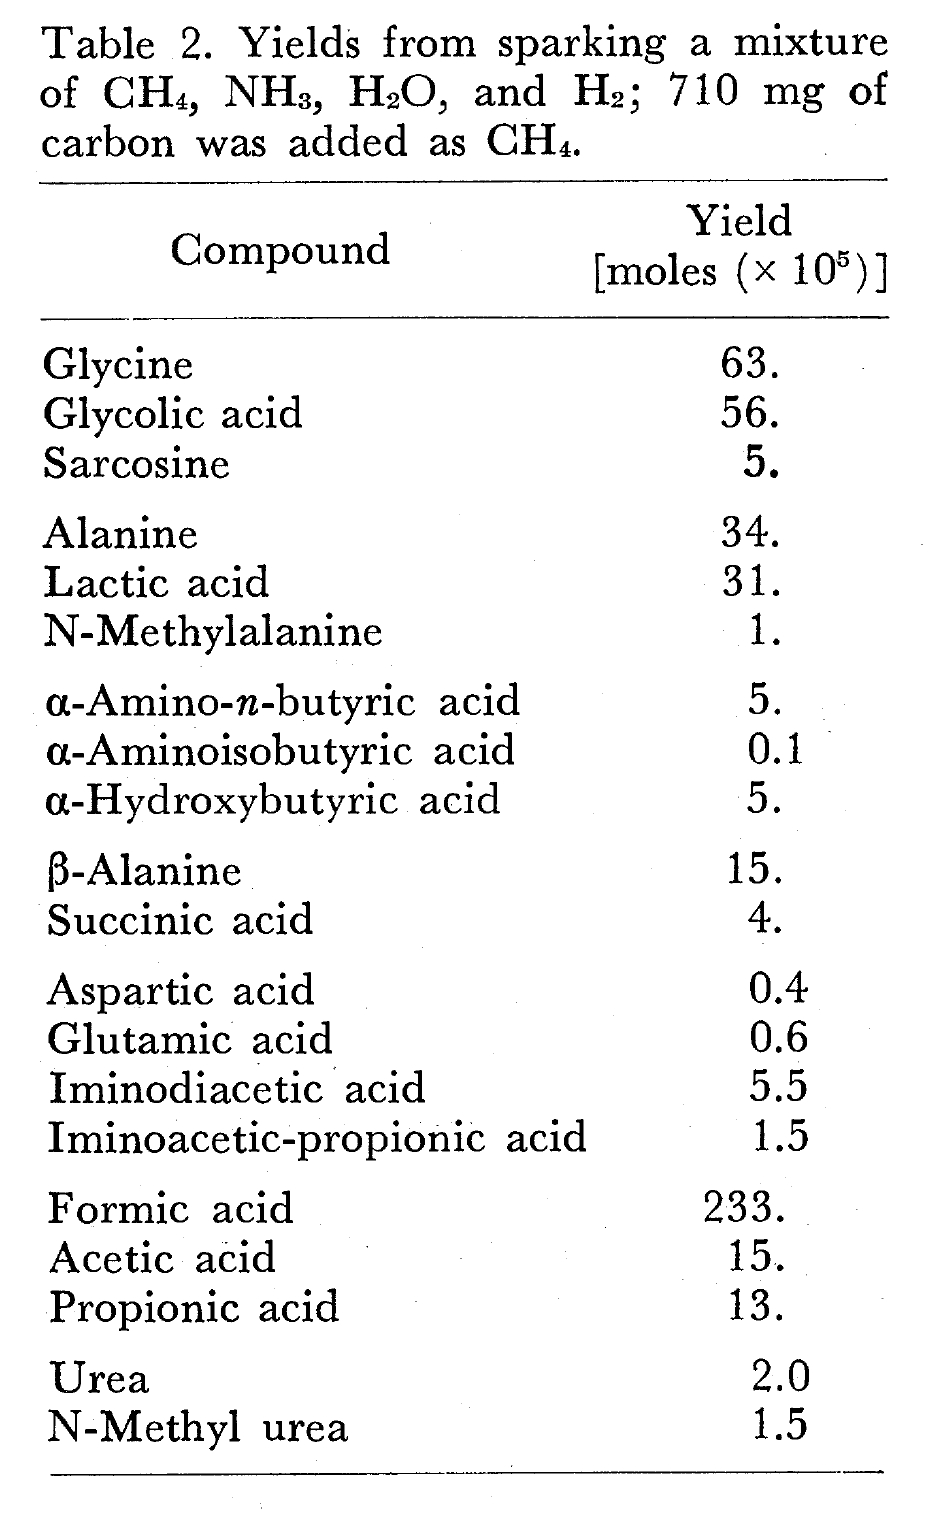
\includegraphics[width=0.45\textwidth]{MillerUrey2}
\end{figure}

The other major source of organic compounds is through interplanetary dust particles--delivery of carbon to Earth from the solar system. When earth was formed the Solar System was still accreting, and smaller particles would have been pulled in by Earth's gravity.  These particles would have had a different chemistry. One of the most famous is the Murchison meteorite--Figure \ref{fig:CarbonaceousChondrites}. It has an interesting library of compounds, including amphiphiles, which could form membrane structures, polycyclic hydrocarbons, alcohols, and some aliphatic hydrocarbons that have could have been metabolic components. When looking at other carbonaceous chondrites  we see that each meteorite has a different library.
\begin{figure}[H]
	\caption[Carbonaceous Chondrites]{Carbonaceous Chondrites after \cite{ehrenfreund2002astrophysical}}\label{fig:CarbonaceousChondrites}
	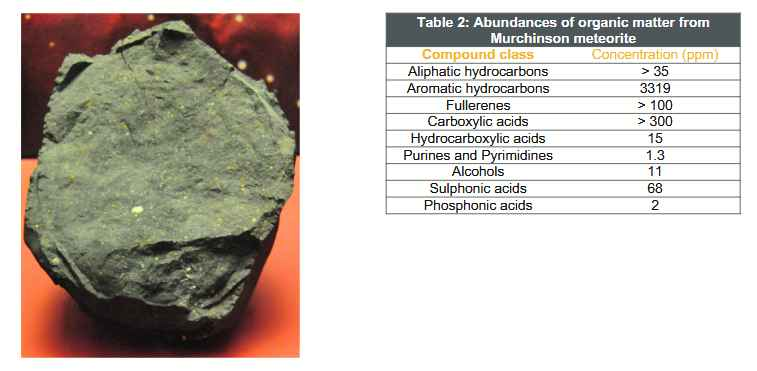
\includegraphics[width=0.8\textwidth]{CarbonaceousChondrites}
\end{figure}


The libraries are produced because the reactions are dependent on the types of energy that hit that particle--Figure \ref{fig:ReactionsInSpace}.

\begin{figure}[H]
	\caption[Reactions In Space]{Reactions In Space after \cite{dalai2016incubating}. UV radiation causes free radicals, which can lead to some strange chemistry.}\label{fig:ReactionsInSpace}
	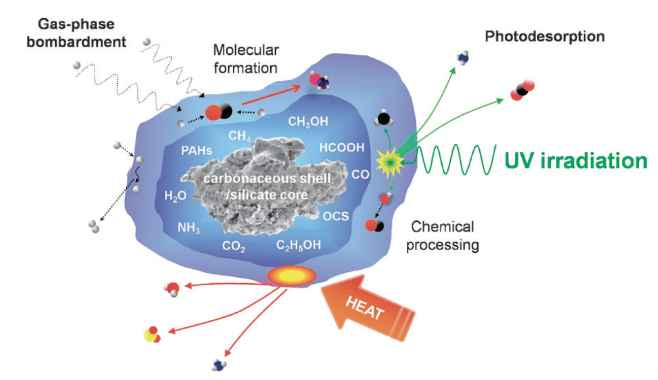
\includegraphics[width=\textwidth]{ReactionsInSpace}
\end{figure}

Was there enough of these reactions to generate a complex chemical that could have led to life? When we estimate how many of all the different events occurred and compile toe different sources of carbon, we estimate about 100 billion kg of prebiotic organic material was delivered to Earth or synthesized on Earth per annum--Figure \ref{fig:SourcesPrebioticOrganicMaterial}. So we think there was enough material to jump-start life.

\begin{figure}[H]
	\begin{center}
		\caption[Sources of Prebiotic of Organic Material]{Sources of Prebiotic of Organic Material after \cite{chyba1997comets}} \label{fig:SourcesPrebioticOrganicMaterial}
		\includegraphics[width=0.8\textwidth]{SourcesPrebioticOrganicMaterial}
	\end{center}
\end{figure}


\subsection[Early Earth Bombardment History]{Early Earth Bombardment History--Nicolle Zellner }

New Views of the Bombardment of the Earth-Moon System, and their effect on our interpretation of the origin of life.

\subsubsection{Why study the Moon?}
\begin{itemize}
	\item Samples and surface are (mostly) undisturbed: no water, no plate-tectonics, no atmosphere.
	\item Samples can be dated ($^{40}Ar/^{39}Ar$, $^{87}Rb/^{87}Sr$, Uranium/Lead etc.)
	\item Craters can be counted, and we can look at superposition of ejecta to estimate age.
\end{itemize}
Lunar cratering rate anchors the impact chronology for the entire (inner) Solar System. We can scale impact fluxes and apply to the other planets.

Figure \ref{fig:LunarImpactFluxModels} shows a number of scenarios.
\begin{figure}[H]
	\caption[Lunar Impact Flux Models]{Lunar Impact Flux Models\cite{zellner2002geochemistry,hartmann1965terrestrial,hartmann1970lunar,hartmann2000time,tera1974isotopic,gomes2005origin}}\label{fig:LunarImpactFluxModels}
	\begin{subfigure}[t]{0.45\textwidth}
		\caption{As we understand solar system formation, there should be a lot of material falling in early, but it starts to decline in intensity going forward.}
		\includegraphics[width=0.8\textwidth]{LunarImpactFluxModelMonotonicDecline}
	\end{subfigure}
	\begin{subfigure}[t]{0.45\textwidth}
		\caption{When the first Lunar samples were dated using Uranium/Lead, we saw a spike instead, known as the Cataclysm, or Late Heavy Bombardment.}
		\includegraphics[width=0.8\textwidth]{LunarImpactFluxModelsWithLHB}
	\end{subfigure}
	\begin{subfigure}[t]{0.45\textwidth}
		\caption{Some investigators now believe there was a series of intense bombardments, with the LHB merely the last one}
		\includegraphics[width=0.8\textwidth]{LunarImpactFluxModelsEIBplusLHB}
	\end{subfigure}
	\begin{subfigure}[t]{0.45\textwidth}
		\caption{New understandings of Solar System Dynamics, plus younger material appearing in Lunar samples has given rise to a 4th scenario, the Sawtooth.}
		\includegraphics[width=0.8\textwidth]{LunarImpactFluxModelsNice}
	\end{subfigure}
\end{figure}

\begin{figure}[H]
	\caption[Importance of Lunar Impact Flux Models]{It is important to understand the Lunar Flux, because we start to see evidence for a cool early Earth (water and continents) and of life.}\label{fig:LunarImpactFluxModelsLife}
	\includegraphics[width=0.8\textwidth]{LunarImpactFluxModelsLife}
\end{figure}

The Lunar Impact Flux allows us to constrain some of the evidence that we see in this early period. There are various ways to interpret the time-varying impact flux
\begin{itemize}
	\item Samples
	\begin{itemize}
		\item crystalline melts in Apollo samples
		\item crystalline melt casts in meteorites
		\item zircons
		\item lunar impact glass (Nicolle's speciality: the glasses retain a memory of the impact.)
	\end{itemize}
	\item Other
	\begin{itemize}
		\item crater counting
		\item stratigraphy
	\end{itemize}
\end{itemize}

Figure \ref{fig:TheCataclysm} shows the Lunar near side, showing that the ages of many of the features are around 4.9 Ga.
\begin{figure}[H]
	\caption[ Lunar near side]{ Lunar near side: U-Pb ages Stratigraphy; Crater counting; A15, A17 breccia; 40Ar/39Ar ages}\label{fig:TheCataclysm}
	\includegraphics[width=0.8\textwidth]{TheCataclysm}
\end{figure}

\begin{figure}[H]
	\caption[Lunar meteorites]{Lunar meteorites. While there is no spike at 3.9Ga, there is little or no evidence of meteorites older than this date.}
	\includegraphics[width=0.8\textwidth]{LunarMeteorites}
\end{figure}

What could account for this cataclysmic event? Figure \ref{fig:nice:model} depicts the Nice Model, where the giant planets did not form in their current positions. When they reached a resonance they shook up the Kuiper Belt.

\begin{figure}[H]
	\caption{The Nice Model}\label{fig:nice:model}
	\begin{subfigure}[b]{0.3\textwidth}
		\caption{Early configuration, before Jupiter and Saturn reach a 2:1 resonance (JSNU)}
		\includegraphics[width=\textwidth]{Nice1}
	\end{subfigure}
	\begin{subfigure}[b]{0.3\textwidth}
		\caption{Objects scatter into the inner Solar System after the orbital shift of Neptune (dark blue) and Uranus (lt. blue)}
		\includegraphics[width=\textwidth]{Nice2}
	\end{subfigure}
	\begin{subfigure}[b]{0.3\textwidth}
		\caption{Current-ishSolar System, after ejection of objects by planets (JSUN)}
		\includegraphics[width=\textwidth]{Nice3}
	\end{subfigure}
\end{figure}

But now we have very high resolution data from the Lunar Reconnaissance Orbiter--Laser Altimeter data and camera data. We also have new interpretations of the Apollo data, more data, and improved analytical techniques. Grange et al looked at some of the samples from 3.9 Ga--Figure \ref{fig:IsotopeRecalibrations}--and found they had roughly the same composition and the same age. They attribute all these sample to one event--Imbrium--Figure \ref{fig:TheCataclysm}. The proposed that Imbrium material contaminated the entire near side of the Moon, hence all the Apollo landing sites.
\begin{figure}[H]
	\caption{Isotope Recalibrations}\label{fig:IsotopeRecalibrations}
	\includegraphics[width=0.8\textwidth]{IsotopeRecalibrations}
\end{figure}

Comparing Figures \ref{fig:UpdatedBasinAges} and \ref{fig:TheCataclysm}, we see that we are now attributing a much wider variation to the ages.
\begin{figure}[H]
	\begin{center}
		\caption[Updated Basin Ages]{Updated Basin Ages(based on new calibrations and superpositioning of ejecta blankets from orbital data). Imbrium’sage is based on Apollo 14 and Apollo 15 samples, whose geologic provenance is not well-established.}\label{fig:UpdatedBasinAges}
		\includegraphics[width=0.8\textwidth]{UpdatedBasinAges}
	\end{center}
\end{figure}

More recently the Gravitometric Data from the \gls{gls:GRAIL} satellite--Figure \ref{fig:GrailData}-- has found
\begin{itemize}
	\item Multiple new basins w/>300km diameters
	\item 6 known basins with D>200km larger than previously measured, hence
	\item crater size frequency distribution needs to be recalibrated and the impact flux changes
\end{itemize}

\begin{figure}[H]
	\caption{Grail Data}\label{fig:GrailData}
	\includegraphics[width=0.9\textwidth]{GrailData}
\end{figure}

We now have evidence for Archaen impacts--Figure \ref{fig:ArchaeanImpactsOnEarth}--so the Late heavy Bombardment lasted longer than we thought. Multiple impact spherule layers from large distal impacts between 3.5 and 3.2 Ga

\begin{figure}[H]
	\caption{Archaean Impacts On Earth}\label{fig:ArchaeanImpactsOnEarth}
	\includegraphics[width=0.9\textwidth]{ArchaeanImpactsOnEarth}
\end{figure}

We have more sensitive instruments and can look at smaller samples than before:
\begin{itemize}
	\item Apollo 16 impact breccia U-Pbage: large event at $4.22\pm0.01Ga$ 
	\item Apollo 16 melt 40Ar–39Ar ages: $4.21\pm0.05$ Ga and  $4.29\pm0.04$ Ga
	\item Lunar zircon heating events w/U–Pbages:  $4.3\pm0.01$,  $4.2\pm0.01$, and  $3.9\pm0.01$ Ga
\end{itemize}

This is pointing to impacts before 3.9 and after 3.9, so that narrow cataclysmic spike probably didn't happen.

\begin{figure}[H]
	\caption{Lunar Flux as a function of Age}\label{fig:LunarFlux}
	\begin{subfigure}[t]{0.30\textwidth}
		\caption{Histogram showing probability of sample having a given age.}
		\includegraphics[width=0.8\textwidth]{LunarFlux0}
	\end{subfigure}
	\;
	\begin{subfigure}[t]{0.30\textwidth}
		\caption{Suppressing the Imbrium contamination gives more of a sawtooth}
		\includegraphics[width=0.8\textwidth]{LunarFluxWithoutImbrium}
	\end{subfigure}
	\;
	\begin{subfigure}[t]{0.30\textwidth}
		\caption{Impacts relatively quiet during Great Oxidation Event, and also during first whiffs of oxygen on earth. Has bombardment picked up on right, or is it just better preserved?}
		\includegraphics[width=0.8\textwidth]{LunarGOE}
	\end{subfigure}
\end{figure}


Interesting things are happening on Earth at this time.

\begin{itemize}
	\item C isotope evidence for life:
	\begin{itemize}
		\item  $>4.0$ Ga, Biogenic carbon in zircons (Bell et al. 2015)
		\item 3.95 Ga, Canada (Tashiroet al. 2017)
		\item 3.85 Ga, Akilia, Greenland (Mojzsiset al.1996)(though highly contested in the literature)
		\item 3.8 Ga, Isua Greenland (Schidlowski, 1988)
	\end{itemize}
	\item Fossil evidence for life: 
	\begin{itemize}
		\item 3.77 Ga, marine hematite tubes(Dodd et al. 2017)
		\item 3.48 Ga, terrestrial palisade fabric
	\end{itemize}
\end{itemize}

Early Life on Earth

\begin{itemize}
	\item Impacts were not very frequent but were prolonged (~4.1 to 3.2 (or younger) Ga)
	\begin{itemize}
		\item No impact frustration(Maher and Stevenson, 1988)
		\item No impact sterilization(Sleep et al. 1989; Nisbetand Sleep, 2001)
		\item A cool early Earth(Wilde et al., 2001; Watson and Harrison, 2005)
		\item Delivery of CHONPS(e.g., amino acids, sugars)
	\end{itemize}
	\item Impacts did affect life but still it persisted
\end{itemize}

\section{Likely Environments for Studying Origins of Life}

\subsection[Likely Environments for Studying Extremophiles]{Likely Environments for Studying Extremophiles-- Nancy Merino}

One of the research areas I think about is the likely environments for studying origins of life.
In order to do this, we have to first understand
what it might have been like on Early Earth billions of years ago.
Then, once we have an idea of that, we can look around on Earth today for similar environments and search for life.

The idea is that we can find clues about early life within modern day life --much like how your own life is a reflection of your own personal history and family's history.
Life probably started
around 4.4 to 3.8 billion years ago. The origins of life is still
a highly debated topic,
so the range still covers
billions of years.
This is what's shown here
in the timeline of Earth's history,
from its formation
about 4.5 billion years ago
to the current times--Figure \ref{fig:LifeProbablyStarted}.


\begin{figure}[H]
	\caption[Life probably started between 4.4 to 3.8 billion years ago]{Life probably started between 4.4 to 3.8 billion years ago (Ga) \cite{domagal2016astrobiology}} \label{fig:LifeProbablyStarted}
	\includegraphics[width=0.9\textwidth]{LifeProbablyStarted}
\end{figure}

There are four different eons of Earth,
known as the Hadean, Archean
and Proterozoic and Phanerozoic Eons.
These are all major time periods
marked by drastic changes
in the Earth's environment.

It's believed that life originated
some time during the Hadean
and Archean Eon.
And, during this time,
there is also probably a lot of comet
and meteorite impacts -
and this is what's known as
the "Late Heavy Bombardment."
These comets and meteorite impacts
would have influenced
the Early Earth environment
because there were just so many of them.
It is one reason why some scientists think
that life may not have started
during the Hadean Eon
because it was extremely hot
and probably inhospitable for life.
Figure \ref{fig:HadeanInhospitable} is an image showing
what it might have looked like on Earth
during the Hadean Eon.
But, this is still a highly debated topic
because we don't have
a really good rock record.
However, we do know that Early Earth
was probably an extremely hot
environment.
\begin{figure}[H]
	\caption[Earth during the Hadean Eon was probably very inhospitable]{Earth during the Hadean Eon was probably very inhospitable for life} \label{fig:HadeanInhospitable}
	\includegraphics[width=0.9\textwidth]{HadeanInhospitable}
\end{figure}

There were also magma oceans.
So, instead of water,
the Early Earth oceans
were made of magma.
These magma oceans started
because of several reasons,
\begin{itemize}
	\item one of which is comet and meteorite impacts, which heated up the surface of the Earth.
	\item Another is tidal heating, which has influences from how close the Moon is to the Earth.
	\item Another is core formation,
	where comet and meteor impacts
	will deposit metals
	onto the surface of the Earth,
	and this will begin sinking
	towards the inner layers of the Earth,
	helping to form the Earth's core.
	This process is known
	as "plate tectonics"--Figure \ref{fig:PlateTectonics}.
\end{itemize}

\begin{figure}[H]
	\caption{Plate Tectonics could have started
		as early as 3.8 billion years ago}\label{fig:PlateTectonics}
	\includegraphics[width=0.8\textwidth]{PlateTectonics}
\end{figure}
So, Earth has a thin surface layer,
which is cracked and can move around.
This is the reason for earthquakes,
and it is also essentially
the recycling of Earth's surface
with the inner parts of the Earth.
This process could have started
as early as 3.8 billion years ago
and is definitely occurring
around 3.2 billion years ago.
This motion most likely helped make
the Early Earth environment
more favorable for life
by helping to cool down the Earth.

In addition to influencing
the origins of life,
plate tectonics also influenced
the evolution of life
through the creation
and movement of continents.
A necessary requirement
for plate tectonics is water.

\begin{figure}[H]
	\caption[Formation of Oceans]{Before plate tectonics really got started,
		oceans probably started to form
		during the Hadean Eon.}\label{fig:FormationOfOceans}
	\includegraphics[width=0.8\textwidth]{FormationOfOceans}
\end{figure}
Before plate tectonics really got started,
oceans probably started to form
during the Hadean Eon.
But, it is not until the Archean Eon
that there are really global oceans
covering the surface of the Earth.
This water didn't just come from nowhere
and there were at least
three sources of water.

\begin{itemize}
	\item One is from plate tectonics influencing the amount of water on Earth's surface.
	
	\item Another source is from volcanoes, which were very active at this time
	and would have helped the conversion of water vapor into liquid.
	
	\item The third source is from delivery by comets and asteroids,
	which are rich in ice.
	
\end{itemize}

Water is definitely one of the most
important substances
at this time to help start life
and is really the main criteria
for life on Earth.
For example,
water plays an important role
in the stability and dynamics
of life's major compounds -
like proteins and \gls{gls:DNA}.

Life took hold on Earth during the Archean Eon--Figure \ref{fig:Chemolithoautotrophs}. There were a mix of things going on
at this time,
which made it possible.
This includes a not so hot environment,
mainly due to the cooling of Earth
by plate tectonics and other processes -
the formation of a global ocean
and the collection of the necessary
ingredients on Early Earth
to actually build a cell-like shape.
\begin{figure}[H]
	\caption{Life took hold on Earth during the Archean Eon} \label{fig:Chemolithoautotrophs}
	\includegraphics[width=0.9\textwidth]{Chemolithoautotrophs}
\end{figure}

However, life during the Archean Eon
had to survive without oxygen.
The atmosphere probably had nitrogen,
carbon dioxide, water
and some amounts of sulfur,
methane and ammonia.
The atmosphere during this time
is actually still highly debated,
but scientists agree
that Early Earth atmosphere
during this time had no free oxygen.
This atmosphere is very much different
from today's atmosphere,
which has 21 percent oxygen.

The earliest life-forms were probably
what we call "chemolithoautotrophs."
The first part of this word
is "chemolitho,"
and that's short for chemolithotroph.
This is Greek for "rock-eater,"
and it means
that the earliest life-forms
probably used inorganic compounds -
for example, iron or sulfur
to get energy.
The second part of this word
is "autotroph."
This means that the first cells
used carbon dioxide for getting carbon.

Carbon is the necessary building material
for our cells,
And so, the Archean Eon essentially had
all the necessary ingredients for life.

We know that life probably took hold
in the Archean Eon
because there is evidence of life
in the rock record.
The first likely signs of life
in the rock record
starts around 3.5
to 3.3 billion years ago.
Figure \ref{fig:EvidenceOfLife} depicts a rock in Western Australia,
which dates back to that time.

\begin{figure}[H]
	\caption[Archaean microfossil
	from a rock in Western Australia]{Here is an image showing a microfossil
		from a rock in Western Australia, which dates back to that time.}\label{fig:EvidenceOfLife}
	\includegraphics[width=0.8\textwidth]{EvidenceOfLife}
\end{figure}
Now we have an idea
of what Early Earth was like,
in now - in modern times -
we are faced with the task
of deciphering the origins
and evolution of life.
How can we think about early life
right now?
To build on top of that,
how can we think about life
on other planetary bodies?
And, modern day Earth
actually has some answers for us.

\begin{figure}[H]
	\caption[A selection of Extreme Environments]{The Earth today is covered
		with many modern-day analogues
		for Early Earth
		and other planetary bodies.}\label{eq:ExtremeEnvironments}
	\includegraphics[width=\textwidth]{ExtremeEnvironments}
\end{figure}
The Earth today is covered
with many modern-day analogues
for Early Earth
and other planetary bodies.
These are all extreme environments.
This image here shows the locations
where microorganisms
have been discovered
all the way from the deep parts
of the ocean
to the Arctic and to volcanoes.

All of these environments
have some kind of extreme component
that requires microbes to have
the necessary adaptations to survive.
So, by studying these environments,
it allows scientists to understand
how microbes can adapt to
extreme environments
and how they might have lived
on Early Earth,
and the potential for life
on other planetary bodies.
Many microbes have been identified
in these extreme environments,
and the microbes that can survive
under extreme conditions
are known as "extremophiles."

Extremes include temperature, pH,
salinity, pressure,
desiccation - or extreme dryness -
and radiation tolerance.
Here are five microscope images
of microbes that can survive
under the most extreme conditions,
and these are the current record holders.

\begin{figure}[H]
	\caption[Five Extremophiles]{Here are five microscope images
		of microbes that can survive
		under the most extreme conditions,
		and these are the current record holders}\label{fig:Extremophiles}
	\includegraphics[width=0.8\textwidth]{Extremophiles}
\end{figure}

So, for example,
Methanopyrus kandleri can grow
at temperatures
up to 122 degrees Celsius -
so this is way above boiling water.
But, because of high pressure,
the water where this microbe
is naturally found does not boil -
and so, this microbe can survive
both high temperatures and high pressure.
And, because it can survive
multiple extremes,
it's also known as
a "polyextremophile."

\begin{figure}[H]
	\begin{center}
		\caption{Life on Earth could potentially survive
			under even more extreme conditions}\label{fig:EarthLifeExtremes}
		\includegraphics[width=0.8\textwidth]{EarthLifeExtremes}
	\end{center}
\end{figure}
Life on Earth could potentially survive
under even more extreme conditions.
Figure \ref{fig:EarthLifeExtremes} is showing
temperature, pH,
pressure and salinity on different axes.
The temperature ranges from minus 300
to 500 degrees Celsius,
the pH ranges from minus 4 to 14,
the pressure ranges from zero
to 1000 megapascals
and salinity ranges from zero
to 50 percent.
The minimum and maximum
for each parameter
is plotted for life on Earth,
and so we can see the space
in which life on Earth occupies.
Now, when we look at all the known
extreme environments on Earth,
we can see there is potential
to push the boundaries of life
on Earth even further.
For example, the maximum temperature
life can grow at
is currently 122 degrees Celsius,
but Earth's environments can reach
to much higher temperatures.
It may not be possible for life to survive
at 400 degrees [Celsius],
but there is potential for microbes
to survive a bit hotter temperatures
than 122 degrees [Celsius].
So, there are many unexplored
regions of Earth
where new microbes
have yet to be discovered.

\begin{figure}[H]
	\caption{What About Other Planetary Bodies?}\label{fig:WhatAboutOtherPlanetaryBodies}
	\includegraphics[width=\textwidth]{WhatAboutOtherPlanetaryBodies}
\end{figure}
But, what about other planetary bodies?
When we look at
the environmental conditions
on the planets Mars, Venus
and the dwarf planet Ceres,
as well as the icy moons Titan,
Enceladus and Europa,
we can see that there are some portions
of those planetary bodies
which match up to the environmental
conditions on Earth.

So, by studying the modern-day analogues
on Earth,
we can further understand life itself
and also explore life in the Universe.


\subsection{Cuatro Ci\'enegas Special Feature}

This is a short film about the people and places of the Cuatro Ci\'enegas Basin in Coahuila, M\'exico.\footnote{This is the transcript from the video, with a few small edits.} The Cuatro Ci\'enegas Basin--its water and microbial, plant and animal communities--are a treasure of M\'exico-Figures \ref{fig:CuatroCienegasMap}, \ref{fig:CuatroCienegas1} \& \ref{fig:ma_0703_NF_CuatroCienegas_aerial_1280}. All of this unique life has been uncovered through the work of Mexican scientists with international collaborations. This work makes possible a deeper understanding of the history of all of life on earth.

\begin{figure}[H]
	\caption[Map of the Cuatro Ci\'enegas Basin]{Map of the Cuatro Ci\'enegas Basin\cite{perezortega2020pools}}\label{fig:CuatroCienegasMap}
	\includegraphics[width=0.9\textwidth]{CuatroCienegasMap}
\end{figure}

\begin{figure}[H]
	\caption{The Cuatro Ci\'enegas Basin}\label{fig:CuatroCienegas1}
	\includegraphics[width=0.9\textwidth]{CuatroCienegas1}
\end{figure}

\begin{figure}[H]
	\caption[Aerial View of the Cuatro Ci\'enegas Basin]{Aerial View of the Cuatro Ci\'enegas Basin\cite{perezortega2020pools}}\label{fig:ma_0703_NF_CuatroCienegas_aerial_1280}
	\includegraphics[width=0.9\textwidth]{ma_0703_NF_CuatroCienegas_aerial_1280}
\end{figure}

\subsubsection{Introduction: Valeria Souza}

My name is Valeria Souza. I work as a researcher at \gls{gls:UNAM}, which is a very large university. This is probably the most important site
that we have in the world right now to understand the origin of diversity. This place has an amazing geology that you can see just in front of you.\cite{souza2018lost}

We have a tsunami of rocks that uplifted--Figure \ref{fig:CuatroCienegas2}--because the mountain that is over that edge is like an arrow. It has an active fault
with magma underneath. And, it's pushing all the marine sediments that are from this valley up and then it's flipped and makes a heart shape--a 3,000 meter mountain.

\begin{figure}[H]
	\caption[A tsunami of rocks]{A tsunami of rocks. The mountain has an active fault
		with magma underneath. And, it's pushing all the marine sediments that are from this valley up and then it's flipped and makes a heart shape}\label{fig:CuatroCienegas2}
	\includegraphics[width=0.9\textwidth]{CuatroCienegas2}
\end{figure}



So, all this amazing geology is an explanation of why Cuatro  Ci\'enegas is a singularity--because these marine sediments store the conditions of the ancient sea. They store the magma that is rich in sulphur, that takes us all the way back to the \gls{gls:archean}, and it stores the minerals that formed in sand. These minerals are very old.

Also, it is a sediment that is devoid of the most basic element for life, that is, phosphorus. So, this site is amazingly poor in phosphorus, and that makes for a very
skewed stoichiometry. Most of life now cannot live in a skewed \gls{gls:stoichiometry}-- we need 60 nitrogens for each phosphorus. Here, we have 100 nitrogens--at least--for each phosphorus, in some places 200 nitrogens for each phosphorus.

So, how they can make basic things, such as ribosomes or \gls{gls:DNA}, is because they are really good at stealing phosphorus from anybody else, including rocks. So, they have an amazing array of strategies to deal with the lack of phosphorus, and they did that since the Archean.

So, here we have \glspl{gls:stromatolite} and microbial mats, whose ancestry goes back
to the Precambrian in some cases--Figure \ref{fig:ma_0703_NF_CuatroCienegas_stromatolite_1280}. And, we are going to a site where we think we have the boundary between the Archean and the Precambrian\footnote{Should this be Proterozoic?}. Since this is a blue pool, we are talking about the moment where animals turned the planet blue, and that was in the \gls{gls:ediacaran} in the late Precambrian.

\begin{figure}[H]
	\caption[Stromatolites at Cuatro Ci\'enegas]{Stromatolites at Cuatro Ci\'enegas \cite{perezortega2020pools}}\label{fig:ma_0703_NF_CuatroCienegas_stromatolite_1280}
	\includegraphics[width=\textwidth]{ma_0703_NF_CuatroCienegas_stromatolite_1280}
\end{figure}

\subsubsection{Microbial Mats: Maria Kalambokidis}
My name is Maria Kalambokidis, and I'm an intern for a year, working in Valeria's lab in \gls{gls:UNAM}, in the Department of Evolutionary Ecology. And, right now, we're at Pozas Azules, at the site of the Archaean domes. 

\begin{figure}[H]
	\caption[A microbial mat showing the activity of  methanogens]{A microbial mat that created a bubble through the activity of  methanogens} 
	\includegraphics[width=0.9\textwidth]{CuatroCienegas3}
\end{figure}

So, here you have a microbial mat that created a bubble through the activity of the methanogens. It created a bubble and then it eventually burst, creating this perimeter. So, we sampled the microbial mats that are still present there. And, right now, they're hidden beneath the salt crust, because it's so dry. My research is looking at the evolutionary resilience of the microbial mats at Cuatro i\'enegas.

So, the microbial mats create a codependent community where each layer is sort of representing the history of metabolisms on Earth--Figure \ref{fig:MicrobialMatDetail}. So, you start with methanogens, 
which create nutrients for the next layer of sulfur-oxidizing bacteria, all the way up until photosynthesis. So, through this community, they've become really dependent on each other and they evolve together, creating a really resilient community in Cuatro  Ci\'enegas that has existed for many millennia.

\begin{figure}[H]
	\caption{The microbial mats create a codependent community}\label{fig:MicrobialMatDetail}
	\includegraphics[width=0.8\textwidth]{MicrobialMatDetail}
\end{figure}

I was interested in the microbial mats because they're evolutionary resilient
and they've existed so long here, but also because they've existed in an environment that many other organisms couldn't exist. For example, a really low nutrient content, in particular, low in phosphorus, which is thought to be necessary for the building blocks of life.

So, they've existed for so long, they're able to exist in extreme environments. Therefore, it creates a sort of living laboratory of organisms that are alive today and indicative of communities that existed long ago. So, in origin of life research and in astrobiology, usually you're looking for signs of life - like biosignatures on another planet, or you're breaking open old rocks to see if there are compounds indicative of life. But, in Cuatro  Ci\'enegas, and in these mats, we think that we have the organisms that formed the same communities that existed long ago.  So, as a biologist, it's really exciting to actually be able to study it alive today.

\subsubsection{Churince System, Intermediate Lagoon: lost due to unmanaged surface and groundwater extraction}
The big questions why so many species on planet Earth or in this place
???the history of survival???

The origin of life was probably very easy.

The origin of life was probably ??????
millions of ways possible???

On this planet, life survived???

???? the rocks
and transformed all of the minerals.???
\subsubsection{Dra. Gabriela Olmedo Alvarez}
My name is Gabriela Olmedo-Álvarez, and I work at Cinvestav: ''center of research for advanced studies.'' I'm in Mexico, right in the middle of Mexico - in Irapuato. I'm the director of Cinvestav in Irapuato, although I am also a researcher. And, I've been working for 15 years, close to Valeria Souza, in trying to decipher what are the keys that allow so much diversity of microorganisms inhabit these places.

\begin{figure}[H]
	\caption{Pond with few nutrients but plenty of life.} 
	\includegraphics[width=0.9\textwidth]{CuatroCienegas4}
\end{figure}

And, if you are looking at the pond behind me - that's a beautiful pond, and it looks like it doesn't have much, because it doesn't have a lot of nutrients. That is why it's so interesting - it doesn't have nutrients, but it has lots of different bacteria, and has evidence of very old life.

It also has these stone-like things that are stromatolites. Stromatolites are evidence of the first types of life on the planet, but here they are still alive. They are still, you know, blooming, and it's very interesting because these are very, very old types of life. And, that is possible precisely because there are no nutrients. So, other larger things
cannot compete with it, and that allows these to remain for centuries and millions of years.


But if we walk just a few meters away, maybe just 200 meters, we'll find a very different scenery. We'll find these very salty crusts, and these salty crusts are full of life also - a very special life with lots of salt and with a low pH. So, it's a weird life that we do not understand, and that's sort of one of the focuses that we have for this trip - to be able to sample what things are living there. And, we'll take them to the lab to figure out how some bacteria or archaea can live with these very, very extreme environments.

\begin{figure}[H]
	\caption[These salty crusts are full of life also]{These salty crusts are full of life also - a very special life with lots of salt and with a low pH.} 
	\includegraphics[width=0.9\textwidth]{CuatroCienegas5}
\end{figure}

\subsubsection{Pozas Rojas: Valeria Souza}

In the system called ''Pozas Rojas'', because these ponds are fluctuating environments, they get very saline in the summer because the water evaporates--Figure \ref{fig:PosasVS}. It is deep water, not rain water, so each one becomes a more vivid color than in winter, where water doesn't evaporate as much--so they get like the juiciness concentrated in the summer.

\begin{figure}[H]
	\begin{center}
		\caption{Valeria Souza at Pozas Rojas}\label{fig:PosasVS}
		\includegraphics[width=0.8\textwidth]{PosasVS}
	\end{center}
\end{figure}

The life that lives here is very diverse - there's microbial mass that we have sequenced--Figure \ref{fig:PosasBiodiversity}.

\begin{figure}[H]
	\begin{center}
		\caption[The life that lives here is very diverse]{The life that lives here is very diverse--there's microbial mass that we have sequenced.}\label{fig:PosasBiodiversity}
		\includegraphics[width=0.8\textwidth]{PosasBiodiversity}
	\end{center}
\end{figure}

There's a very large biodiversity and there are like islands. There are nine small islands of these tiny \gls{gls:poza}s and a big lagoon--Figure \ref{fig:CuatroCienegas7}.

\begin{figure}[H]
	\caption{There are nine small islands of these tiny \gls{gls:poza}s and a big lagoon.}\label{fig:CuatroCienegas7} 
	\includegraphics[width=0.9\textwidth]{CuatroCienegas7}
\end{figure}

So, you can compare the diversity in each one of them separately and then the big \gls{gls:poza} in the middle. But, this was perturbed by a hurricane in 2010 and it became a complete lake, all of its... It kind of drained all the nutrients and all the water from the... east side of the valley. The biology changed because the \gls{gls:poza}s became connected 
with the lake water, and also the nutrients changed. It was - before the hurricane - it was the site with less phosphorus. Now, it is a site that nearly has a balance of stoichiometry. So, it is very interesting how the life got habituated to this richer environment. What is even more interesting is that what was a very primitive site it became a more Holocene site.

For example, the Vibrio that lives here, they didn't radiate since the Holocene in Cuatro  Ci\'enegas, which is at the same time as the fishes came from the R\`io Bravo shelf. So, they are very interesting, and they are always changing, and that makes us really happy --and we are following their change. So, I'm sure that the deep aquifer still has the deep, ancient bacteria. It shows that the lake that shaped here, that came here, brought newer creatures from everywhere that were bacteria more used to nutrients. And, maybe there are pockets of nutrients in different parts of the valley.

What makes Cuatro  Ci\'enegas unique is precisely the lack of nutrients. Maybe they are going to become--each time that we sample--more and more imbalanced and return to their ancient selves. But, it will take time.

\subsubsection{Jorge Valdivia}

My name is Jorge Valdivia, and I am a full-time professor at the Universidad Nacional Aut\'onoma de M\'exico. [...] of my doctoral studies in the Cuatro  Ci\'enegas valley. I was working with the genus Bacillus and the project was focused on knowing the relationship that existed between the number of copies of the ribosomal operon and with the available phosphorus.
\begin{figure}[H]
	\caption[Variability of the r\gls{gls:RNA} operon copy number]{Variability of the r\gls{gls:RNA} operon copy number in the Bacillus diversity from the Cuatro  Ci\'enegas basin\cite{valdivia2016variability}} 
	\includegraphics[width=0.9\textwidth]{CuatroCienegas8}
\end{figure}

It is known that the valley of Cuatro  Ci\'enegas is an extremely \gls{gls:oligotroph}ic site. With these conditions...they are homologous to what... the conditions in the past [...] origin of life. Then, the interesting thing to find out was how a genus that is characterized by having many copies of the ribosomal operon can adapt to these conditions of extreme oligotrophy.

We wanted to work in the isolates of the main sites in the valley, and we wanted to quantify the genome level - how many ribosomal operons they had. We set them to grow
with water from the site to replicate the natural conditions in which they are found living, and what we observe is that there is a zero correlation with respect to the hypothesis of the growth rate.

\subsubsection{Mostly untranslated}
A good indication are the viruses--Figure \ref{fig:QuatroCinegasViruses}. Viruses are the most ferocious hunters in the world. And, like ferocious hunters, each one has their own favorite prey. And, Cuatro  Ci\'enegas is the most diverse place on the planet for viruses at the tiniest scale. And, the favorite food of those viruses are bacteria.

\begin{figure}[H]
	\caption{A good indication are the viruses.}\label{fig:QuatroCinegasViruses}
	\includegraphics[width=0.8\textwidth]{QuatroCinegasViruses}
\end{figure}

\subsubsection{Nahui Medina: Archaea and extremophiles}
My name is Nahui Medina, and right now I'm a PhD student in Nuevo Le\'on in Monterrey. So, right now I'm doing this amazing project about Archaea and extremophiles. What we do right now is try to isolate every single microorganism that we can, and we do this with amazing people in the lab, trying to create strategies to make these microorganisms live in the lab. This is pretty much interesting because Archaea, you know, in Ancient Greek, is about "ancient," you know. This means that it could help us to know how they lived and try to understand...how life is...what begun... at that moment...it's pretty interesting...

They are so beautiful because they have so many colors - red, pink, and like a... yellowish, some of them. So, it's a pretty amazing project we're doing right now. 
Maybe because it's in a place where the whole ecosystem, and the whole habitat is 
it's not in another place, you know... you cannot find... the species that are in here. So, it's very... interesting because the microorganisms or the prokaryotes are living here. There's just living here and that's it. You cannot find them in another place in the world. So, that's what we're doing and we're so happy to do it.

\subsubsection{Valeria Souza: Posa Azul Two}
\begin{figure}[H]
	\caption{\Gls{gls:poza} Azul Two} 
	\includegraphics[width=0.9\textwidth]{CuatroCienegas9}
\end{figure}

Here we are in \Gls{gls:poza} Azul Two, that is one of the most beautiful \gls{gls:poza}s in all the valley. What we can see behind us is a very big stromatolite shelf. So, these blue \gls{gls:poza}s take us back to 600 million years ago when the animals changed the chemistry of the ocean and the ocean turned blue --and that's called the Ediacaran Era. So, in Cuatro  Ci\'enegas, we have kind of different timeframes - different moments in geology that got preserved. And, that's really interesting because it's not just a metaphor, it's not just that it looks like the Ediacaran, and when the ocean turned blue, and still the stromatolite shelf were being eaten by the first herbivores -- that was their doom.


But also, it's that this lineage has survived - survived for the longest time. In the Archaean domes that are 50 metres over there--Fugure \ref{fig:PozasAzulesDomes}-- we have evidence that the Archaean - a world of methane and CO2 - is preserved inside domes that are built by bacteria that protect the ancient anaerobic bacteria from the oxygen input--Figure \ref{fig:PozasAzulesDomeInside} while they are doing photosynthesis. This kind of cooperation and construction of the whole niche is pretty unique. We know that stromatolite were world-builders - they made the ocean blue, they transformed every element that came from the start and made life complex. For the fact is that, here in Cuatro  Ci\'enegas, we have a window - a true window - of those lost worlds is really incredible.
\begin{figure}[H]
	\caption{In the Archaean domes that are 50 metres over there} 
	\begin{subfigure}[t]{0.45\textwidth}
		\caption{Archaean Domes}\label{fig:PozasAzulesDomes}
		\includegraphics[width=0.9\textwidth]{PozasAzulesDomes}
	\end{subfigure}
	\begin{subfigure}[t]{0.45\textwidth}
		\caption{Inside an Archaean Dome}\label{fig:PozasAzulesDomeInside}
		\includegraphics[width=0.9\textwidth]{CuatroCienegas10}
	\end{subfigure}
\end{figure}
Because you walk... meters and you find three billion years... of time. And, you can have lineages that are very, very divergent from the ones we know now, how they assemble their nutrients and how they work. We can cultivate them, we can study them using metagenomics. But, for them to be studied, we need water. And, this water here is precious -it's not just any water. So, water that comes from that mountain that has a magmatic heart, that magmatic heart is responsible for the Jurassic. So, what happened is - humans - we are really silly, and we think we can manage nature. When there's agriculture in the desert... where the water comes comes from -the deep aquifer. And, it is not just any aquifer - it's an aquifer that has stored the conditions of the early sea, and we are losing it.

\begin{figure}[H]
	\caption[The tragedy of Churince where there's no longer water]{Then we have the tragedy of Churince where there's no longer water} 
	\includegraphics[width=0.9\textwidth]{CuatroCienegas11}
\end{figure}

Then we have the tragedy of Churince where there's no longer water. It only looks like that. And now, it's a field of dead turtles and dead fishes. Maybe there's some hope that we can recover it if we close all the channels that are taking out the water from this ecosystem.

References:  \begin{itemize}
	\item General:
	\begin{itemize}
		\item \cite{souza2018lost} contains an overview of \gls{gls:alphadiversity} at Cuatro  Ci\'enegas, covering both \gls{gls:redqueen} and \gls{gls:blackqueen} effects.
		\item \cite{perezortega2020pools,valdivia2016variability,gomez2018leptolyngbya,taboada2018geographic}
	\end{itemize}
	\item Phosphates \cite{hao2020cycling,elser2006early}
\end{itemize}.

\section[Chemistry and The Origins of Life]{Chemistry and The Origins of Life-- Christopher Butch}


We are talking about the origin of life, so why are we talking about chemistry? Organic Chemistry is the Chemistry of Life--Figure \ref{fig:Organic Chemistry}: our bodies are made of chemicals, and the processes of the body are chemical reactions. In order to understand where \gls{gls:DNA} and \gls{gls:RNA} come from we need to understand chemistry.


\begin{figure}[H]
	\caption {Organic Chemistry is the Chemistry of Life}\label{fig:Organic Chemistry}
	\begin{subfigure}[b]{0.55\textwidth}
		\includegraphics[width=\textwidth]{OrgChem1}
	\end{subfigure}
	\;
	\begin{subfigure}[b]{0.35\textwidth}
		\includegraphics[width=0.6\textwidth]{OrgChem2}
	\end{subfigure}
\end{figure}

The origin of the scientific field of Origin of Life is the Stanley Miller Experiment\cite{ferus2017formation,miller1953production}--Figure \ref{fig:StanleyMillar}.

\begin{figure}[H]
	\begin{center}
		\caption[The Stanley Miller Experiment]{The origin of the scientific field of Origin of Life is the Stanley Miller Experiment}\label{fig:StanleyMillar}
		\includegraphics[width=0.6\textwidth]{StanleyMillar}
	\end{center}
\end{figure}

What molecules does nature provide? We now have information from molecular clouds in the Universe, from robots on Mars, from meteors, and from deep ocean vents--Figure \ref{fig:NaturalExperiments}. We are trying to understand the chemical inventory from which life was built.
\begin{figure}[H]
	\begin{center}
		\caption{Natural Experiments}\label{fig:NaturalExperiments}
		\includegraphics[width=0.8\textwidth]{NaturalExperiments}
	\end{center}
\end{figure}

It's not enough to know the chemical inventory. There is a problem, which Steve Benner calls the ''Tar problem'': Biomolecules plus heat and time $\rightarrow$ black sludge.\cite{benner2012asphalt}

\begin{itemize}
	\item How do we stop this from happening?
	\item How do we produce useful polymers without making black sludge? 
	\item If we produce black sludge can we somehow turn it into something resembling life?
	\item What molecules can be and are created without life?
	\item How can these molecules be made to react in a life like manner?
	\item How can formation of wasteful byproducts like	tars be prevented?
\end{itemize}


See also \cite{lazcano20031953}

\section[Why Nature Chose Phosphates]{Why Nature Chose Phosphates--Chris Butch}


The role of phosphate in biochemistry and the origins of life.

\subsection{The roles of phosphate in biology}

\begin{itemize}
	\item Structural
	\item Physical
	\item Chemical
\end{itemize}

\subsubsection{Structural role of phosphate}

\begin{itemize}
	\item Nucleic Acid Backbones. \gls{gls:RNA} and \gls{gls:DNA} are linked by phospho-diester bonds--Figure \ref{fig:PhosphoDiesterBond}. The reason is linked to a few properties of phosphorus and its negative charge.
	\begin{itemize}
		\item it repels negatively charged nucleophiles--Figure \ref{fig:PhosphoDiesterBond1}, which would try to break the bond. So the bond is very stable.
		\item it is tunable. If the biochemistry requires the bond to be broken, all it needs to do is position something positive nearby--Figure \ref{fig:PhosphoDiesterBond2}. This is also how nucleic acids are synthesized--Figure \ref{fig:PhosphoDiesterBond3}.
		\item Once the strands have been formed, the charge has an important role in the structure of \gls{gls:RNA} duplexes. It turns out that the phosphates on either strand repel each other, helping to keep the duplex more linear, and the phosphates on each strand repel the other one. This has an important role for keeping the nucleic acid soluble, by keeping them from collapsing in on themselves--Figure \ref{fig:PhosphoDiesterBond3}.
	\end{itemize}
	\item Phospholipid Bilayers. These have a hydrophobic end and a hydrophilic end--Figure \ref{fig:PhosphoLipid1}, which typically has a phosphate and a positively charge portion. Because of this split between hydrophobic and hydrophilic, Phospholipids have a tendency to form two dimensional structures--Figure \ref{fig:PhosphoLipid2}. Zooming out we see the phospholipid layer forming the outer wall of a cell--Figure \ref{fig:PhosphoLipid3}.
\end{itemize}


Phosphates when added to a protein cause a conformational change. This can either activate or inactivate the molecule. A great example is in Protein phosphatase 1 which phosphorylates glycogen synthase causing activation, while also phosphorylating phosphorylase kinase making it inactive\footnote{Comment from Sarah Maurer in Firom}.

\begin{figure}[H]
	\caption{Nucleic Acid Backbones}
	\label{fig:three graphs}
	\begin{subfigure}[b]{0.45\textwidth}
		\centering
		\caption{Phospho Diester Bond}\label{fig:PhosphoDiesterBond} 
		\includegraphics[width=\textwidth]{PhosphoDiesterBond}
	\end{subfigure}
	\begin{subfigure}[b]{0.45\textwidth}
		\centering
		\caption{Repels negatively charged nucleophiles which might break bond, so very stable}\label{fig:PhosphoDiesterBond1} 
		\includegraphics[width=\textwidth]{PhosphoDiesterBond1}
	\end{subfigure}
	\begin{subfigure}[b]{0.45\textwidth}
		\centering
		\caption{Bond is tunable if we need to react}\label{fig:PhosphoDiesterBond2} 
		\includegraphics[width=\textwidth]{PhosphoDiesterBond2}
	\end{subfigure}
	\begin{subfigure}[b]{0.45\textwidth}
		\centering
		\caption{Repulsion keeps  soluble and prevents collapse}\label{fig:PhosphoDiesterBond3} 
		\includegraphics[width=\textwidth]{PhosphoDiesterBond3}
	\end{subfigure}
	
\end{figure}
\begin{figure}[H]
	\caption{Phospholipids}\label{fig:PhosphoLipids}
	\begin{subfigure}[t]{0.3\textwidth}
		\centering
		\caption{Phospholipid Bilayers, showing hydrophobic end and a hydrophilic end.}\label{fig:PhosphoLipid1} 
		\includegraphics[width=\textwidth]{PhosphoLipid1}
	\end{subfigure}\;
	\begin{subfigure}[t]{0.3\textwidth}
		\centering
		\caption{ Because of this split between hydrophobic and hydrophilic, Phospholipids have a tendency to form two dimensional structures}\label{fig:PhosphoLipid2} 
		\includegraphics[width=\textwidth]{PhosphoLipid2}
	\end{subfigure}\;
	\begin{subfigure}[t]{0.3\textwidth}
		\centering
		\caption{Zooming out we see the phospholipid layer forming the outwr wall of a cell.}\label{fig:PhosphoLipid3} 
		\includegraphics[width=\textwidth]{PhosphoLipid3}
	\end{subfigure}
	
\end{figure}

\subsubsection{Physical}

\begin{itemize}
	\item Compartmentalization--Figure \ref{fig:Compartmentalization}. By having this charged barrier, biochemistry can determine what can and cannot go into a cell. An example is the reaction of 2 3Carbon to form a 6Carbon--Figure \ref{fig:CompartmentalizationExample}. Although phosphorus isn't involved--the atoms are at the opposite ends of the two chains--the phosphoralization is preserved, and this is a motif. It keeps the sugars inside the cell.
	\item Signaling Some examples of how phosphates are used in signaling are in the signaling cascades where proteins are phosphorylated or cAMP is generated.
\end{itemize}

\begin{figure}[H]
	\caption{Phosphates allow physical Compartmentalization}\label{fig:Compartmentalization}
	\begin{subfigure}[t]{0.35\textwidth}
		\caption{Charged molecules can be stopped, but not uncharged}
		\includegraphics[width=\textwidth]{Compartmentalization}
	\end{subfigure}\;
	\begin{subfigure}[t]{0.5\textwidth}
		\caption{Example: Glycolosis and Gluconeogenesis }\label{fig:CompartmentalizationExample}
		\includegraphics[width=\textwidth]{CompartmentalizationExample}
	\end{subfigure}
\end{figure}
\subsubsection{Chemical}

\begin{itemize}
	\item Energy--Figure \ref{fig:ATP}. ''On any given day you turn over your body weight equivalent in \gls{gls:ATP}, the principal energy currency of the cell''--\cite{tornroth2008opening}. The reason is the energy of the Triphosphate can be used to transfer phosphate to other molecules--Figure \ref{fig:ATP1}
	\item Activation Once you have tranferred phosphorous, it can be used as leading group to promote a reaction that would not otherwise be favourable--Figure \ref{fig:Synthesis-beta-5-phosphorybosylamine}. 
\end{itemize}

\begin{figure}[H]
	\caption{Adenosine Triphosphate}\label{fig:ATP}
	\includegraphics[width=0.8\textwidth]{ATP}
\end{figure}

\begin{figure}[H]
	\caption[ATP transferring phosphate to other molecules]{The energy of the Triphosphate can be used to transfer phosphate to other molecules. Phosphate can also be used in polymerization.}\label{fig:ATP1}
	\includegraphics[width=0.8\textwidth]{ATP1}
\end{figure}

\begin{figure}[H]
	\caption{Synthesis of $\beta$-5 phosphorybosylamine}\label{fig:Synthesis-beta-5-phosphorybosylamine}
	\includegraphics[width=0.8\textwidth]{Synthesis-beta-5-phosphorybosylamine}
\end{figure}


\subsection{Why wouldn't you use phosphate?}

\subsubsection{Phosphate is quite scarce\cite{keefe1995polyphosphates}}
\begin{itemize}
	\item Insoluble, un-reactive (tied up in minerals that are not available for life)
	\item No polyphosphate minerals
	\item One pyrophosphate mineral
	\item Limited geochemical production of reactive forms
\end{itemize}
\subsubsection{Open Questions--\cite{life2017special}}

\begin{itemize}
	\item How did life begin to use phosphate?
	\item When did life begin to use phosphate?
	\item If not at the very beginning, what came before?\cite{goldford2017remnants}
	\item Where did early phosphate come from?
\end{itemize}

See also \cite{westheimer1987nature,soderberg2019organic}

\section{Why Water? Why Carbon?}

\subsection{Why Water? Why Carbon?}

\begin{itemize}
	\item All life on earth is based on reactions of carbon and water.
	\item Why? What are the options?
\end{itemize}

Figures \ref{fig:abundances1} and \ref{fig:abundances2} show abundances. Figure \ref{fig:minerals} shows elements likely to be locked up in minerals, Figure \ref{fig:volatiles} shows elements that are likely to be in atmosphere or sea. Bonds are important - carbon has 4.

\begin{figure}[H]
	\caption{Abundance of Elements in the Solar System}\label{fig:abundances1} 
	\includegraphics[width=0.9\textwidth]{Abundances}
\end{figure}

\begin{figure}[H]
	\caption{Abundance of Elements in the Earth's Crust}\label{fig:abundances2}  
	\includegraphics[width=0.9\textwidth]{AbundancesEarth}
\end{figure}

\begin{figure}[H]
	\caption[Some elements locked in minerals]{Some elements locked in minerals: they react with oxygen and get locked up.}\label{fig:minerals} 
	\includegraphics[width=0.9\textwidth]{AbundancesMinerals}
\end{figure}

\begin{figure}[H]
	\caption{Some elements volatile}\label{fig:volatiles} 
	\includegraphics[width=0.9\textwidth]{AbundancesGases}
\end{figure}

Abundance isn't the only question. We need to talk about how these elements behave at the electronic level--Figures \ref{fig:Behaviour1} and \ref{fig:Behaviour2}. Carbon is:
\begin{itemize}
	\item the element in Figure \ref{fig:Behaviour2} that is most able to form a diverse set of chemistries;
	\item at the temperatures and pressures on the surface of the earth, is able to adopt a number of different bonding strategies.
\end{itemize}

\begin{figure}[H]
	\caption{how these elements behave at the electronic level}
	\begin{subfigure}[t]{0.5\textwidth}
		\caption{Life is bases on HCON}\label{fig:Behaviour1}
		\includegraphics[width=\textwidth]{Behaviour1}
	\end{subfigure}
	\begin{subfigure}[t]{0.4\textwidth}
		\caption{At the simplest level this is based on the number of electrons that are available.}\label{fig:Behaviour2}
		\includegraphics[width=\textwidth]{Behaviour2}
	\end{subfigure}
	\begin{subfigure}[t]{1.0\textwidth}
		\caption{The role of water in polymerization/de-polymerization.}\label{fig:Polymerization}
		\includegraphics[width=\textwidth]{Polymerization}
	\end{subfigure}
\end{figure}

What about water?Polymerization
\begin{itemize}
	\item Hydrogen and oxygen are abundant in the Sun and on Earth;
	\item Water is more stable than $H_2$ and $O_2$;
	\item Water is liquid, which is important for mixing chemical to allow reactivity.
	\item Water is involved in polymerization/de-polymerization--Figure {fig:Polymerization}.
\end{itemize}

Water is abundant, stable, and a liquid.

\subsection{What are the other possibilities?}

\subsubsection{What are the other possibilities instead of carbon?}

\begin{itemize}
	\item Silicon
	\begin{itemize}
		\item Can adopt similar structures to carbon
		\item Poor reactivity with many other elements
		\item Reactive with water
	\end{itemize}
	\item Borane
	\begin{itemize}
		\item Diverse Chemistry
		\item Unstable in Oxidizing Environment
		\item Low Cosmic Abundance
	\end{itemize}
	\item Metal Oxides (?)
	\begin{itemize}
		\item 	Less diverse chemistry
		\item Demonstrated biomimetic functions
	\end{itemize}
\end{itemize}

\subsubsection{What are the other possibilities for solvents?}
\begin{itemize}
	\item Ammonia
	\item Urea
	\item Formamide
	\item Alkanes
\end{itemize}

\subsubsection{Open Questions}
\begin{itemize}
	\item What are the surface and atmospheric chemistries of
	exoplanets?
	\item How much of extant biochemistry can be accomplished
	in other solvents?
	\item How much of extant biochemistry can be mimicked with
	other substrates?
\end{itemize}
\section{Macromolecules}

Sarah Maurer

\subsection{Proteins and Lipids}

\subsubsection{Proteins\cite[25.9 Proteins]{brown2009chemistry}}

Proteins are made up of amino acids--Figure \ref{fig:AminoAcids}. Amino acids can be grouped in various ways, based on their side chain--the orange regions in Figure \ref{fig:AminoAcids}. One way to group them is shown in Figure \ref{fig:AminoAcidsGrouped}, where amino acids are grouped by charge. The different groups have different functionality. It is important to have 20 amino acids, so we have a diverse range of functionality in our end product, the protein.

\begin{figure}[H]
	\caption[The full set of 20 amino acids]{The full set of 20 amino acids: blue atoms form protein backbone, orange the sidechain. There are a couple of extra amino acids used for some organisms, but these are the standard set.}\label{fig:AminoAcids} 
	\includegraphics[width=0.8\textwidth]{AminoAcids}
\end{figure}

\begin{figure}[H]
	\caption{Amino acids grouped by charge: non-polar side chains are strongly carbon containing; uncharged polar the side groups contain oxygen, sulphur or nitrogen, with zero nett charge; charged polar the oxygen or nitrogen is negatively or positively charged. }\label{fig:AminoAcidsGrouped} 
	\includegraphics[width=0.8\textwidth]{AminoAcidsGrouped}
\end{figure}
To get proteins we have to condense two amino acids together--Figure \ref{fig:AminoAcidsCondensed}--by removing a water molecule from the carboxylate and the amine, producing a peptide bond. This can be accomplished by taking an aqueous solution of amino acids and drying them down; this could have happened on early Earth.
\begin{figure}[H]
	\caption{Condensing amino acids by removing $H_2O$. Dehydration.}\label{fig:AminoAcidsCondensed} 
	\includegraphics[width=0.9\textwidth]{AminoAcidsCondensed}
\end{figure}

Proteins have a very specific folded structure--Figure \ref{fig:proteinStructure}--which enables them to recognize their target, a reactant or substrate. The protein and its target fit together like a lock and key: the protein has evolved to match its target.

\begin{figure}[H]
	\caption[Proteins have a very specific folded structure]{Proteins have a very specific folded structure. This example has several $\alpha$-helices and one $\beta$-sheet, represented by an arrow.}\label{fig:proteinStructure}
	\includegraphics[width=0.8\textwidth]{proteinStructure}
\end{figure}

\begin{itemize}
	\item  Need at least several amino acids to have folded stability; most proteins are 50+ amino acids
	\item We would need protein formation to happen many times on early Earth.
	\item Some functional proteins catalyze reactions--either by making or breaking bonds. They are known as "enzymes":
	\begin{itemize}
		\item Lower transition state energy, or;
		\item Orient and concentrate reactants, so they react more quickly than if floating around in solution.
	\end{itemize}
\end{itemize}


\subsubsection{Lipids}

\Glspl{gls:lipid}\cite[14.2 Lipids \& Triglycerides]{brown2009chemistry} are the 2nd type  of biomolecule in this lecture. \glsdesc{gls:lipid}.  \Glspl{gls:lipid} are essential to identifying the individual cells and allow for the cells to undergo Darwinian selection. Lipids form a bilayer--Figure \ref{fig:Lipids}. Water molecules interact with the polar head groups.

\begin{itemize}
	\item \glspl{gls:phospholipid} make up modern cell membranes
	\item other \glspl{gls:amphiphile} can also form membranes
\end{itemize}

\begin{figure}[H]
	\caption[How lipids  allow Darwinian evolution.]{Lipids form hydrophobic membranes that surround cells, and allow Darwinian evolution.}\label{fig:Lipids} 
	\includegraphics[width=0.9\textwidth]{Lipids}
\end{figure}

\begin{itemize}
	\item Most lipids have a glycerol backbone--Figure \ref{fig:LipidTypes}.
	\item You can dehydrate glycerol with a fatty acid to produce glycero fatty acids called glycero esters.
	\item The esters will self assemble into our membranes.
\end{itemize}
\begin{figure}[H]
	\begin{center}
		\caption[Type of lipid depends on head-group]{Type of lipid depends on head-group (blue).}\label{fig:LipidTypes} 
		\includegraphics[width=0.8\textwidth]{LipidTypes}
	\end{center}
\end{figure}
The membrane functionality will depend on the headgroup--Figure \ref{fig:LipidTypes}.

\begin{figure}[H]
	\caption{Chemical Structure of Phospholipids}\label{fig:Phospholipids}
	\includegraphics[width=0.8\textwidth]{Phospholipids}
\end{figure}

\begin{itemize}
	
	\item some membranes in Achaea, are monolayer not bilayer.
	\item Figure \ref{fig:SimplerLipids} shows some example. Left one has been found in meteorites.
\end{itemize}

Simpler Lipids--Figure \ref{fig:SimplerLipids}?
\begin{itemize}
	\item Single chain amphiphiles with  chemically diverse headgroups
	\item Less stable than phospholipids
\end{itemize}

\begin{figure}[H]
	\caption{Early life would have used simple lipids.}\label{fig:SimplerLipids} 
	\includegraphics[width=0.9\textwidth]{SimplerLipids}
\end{figure}

\subsection{Nucleic Acids \& Sugars}

\subsubsection{Sugars}

Sugars are really important, because they are used for storing energy. They play many role in biological systems:
\begin{itemize}
	\item generating and storing biological energy--Figure \ref{fig:SugarsCycle}.
	\item molecular recognition (as in the immune system)
	\item cellular protection (as in bacterial and plant cell 	walls)
	\item maintaining biological structure (e.g., cellulose).
	\item controlling protein trafficking
	\item cell signaling
	\item cell adhesion
	\item biological lubricants
\end{itemize}

\begin{figure}[H]
	\caption{Sugars: generating biological energy and storing it until we are ready to turn it into \gls{gls:ATP}}.\label{fig:SugarsCycle} 
	\includegraphics[width=0.9\textwidth]{SugarsCycle}
\end{figure}

Sugars have a wide range of structures--Figure \ref{fig:SugarsStructure}.

\begin{figure}[H]
	\caption[Variety of D-\glspl{gls:aldose}]{Variety of D-\glspl{gls:aldose}. When there are 4 carbons there is only one possible structure, but there are 8 structures for 6 carbons. These are known as D-sugars because the second to last carbon has the \emph{OH} on the right hand side. The other carbons have every possible variation to make up the number of variants.}\label{fig:SugarsStructure} 
	\includegraphics[width=0.9\textwidth]{SugarsStructure}
\end{figure}

The double bonded oxygen in the first position makes the sugars in Figure \ref{fig:SugarsStructure} into \glspl{gls:aldehyde}. There is a second type of sugar, \gls{gls:ketose}, that has the doubly bonded carbon in the second position--Figure \ref {fig:ketoses}--i.e. they are \glspl{gls:ketone}. There is less variation among ketoses, but we still have the second to last carbon having an OH on the right hand side, making them D-Sugars.
\begin{figure}[H]
	\caption[Variety of D-ketoses]{Variety of D-ketoses. Because C1 and 2 are not chiral centers there are fewer possible forms for ketoses.}\label{fig:ketoses} 
	\includegraphics[width=0.9\textwidth]{ketoses}
\end{figure}

These sugars are not always linear; they are usually not linear in the body.

\begin{itemize}
	\item Ribose--a 5 carbon sugar from Figure \ref{fig:SugarsStructure}--is usually rolled up into \gls{gls:pyran} (6 member ring) or \gls{gls:furan}(5)
	\item Reactive OH group (green in Figure \ref{fig:SugarTautomers}) is called the ''anomeric Oxygen''; it can be at the bottom ($\alpha$) or top($\beta$). This is where polymerization happens. \gls{gls:RNA} uses $\beta$-furanose form of ribose, which is not the most abundant naturally--Figure \ref{fig:SugarTautomers}--so we need enzymes to make this type.
\end{itemize}

\begin{figure}[H]
	\caption[Sugars can accomplish different functions, depending on shape.]{Sugars are usually not linear: can accomplish different functions, depending on shape.}\label{fig:SugarTautomers} 
	\includegraphics[width=0.9\textwidth]{SugarTautomers}
\end{figure}

Sugars can be made prebiotically from the formose reaction--Figure fig:{SugarsPrebioticSynthesis}. We take small formaldehyde molecules and react them the form larger units. Formaldehyde could be made from carbon dioxode or monoxide and hydrogen

\begin{figure}[H]
	\caption[Prebiotic synthesis of sugars: formose reaction]{Prebiotic synthesis of sugars: formose reaction. As the reaction progresses an insoluble “tar” forms an sugar concentrations decrease!}\label{fig:SugarsPrebioticSynthesis} 
	\includegraphics[width=0.9\textwidth]{SugarsPrebioticSynthesis}
\end{figure}


\subsubsection{Nucleic Acids}

Once we have synthesized our sugars, we start to build nucleic acids. To make a nucleic acid you first need a base--Figure \ref{fig:Nucleobases}. The nitrogen makes these molecules basic.

\begin{figure}[H]
	\caption[The heterocyclic bases are
	derivatives of \gls{gls:purine} and of \gls{gls:pyrimidine}]{The two types of heterocyclic bases are
		derivatives of \gls{gls:purine} and of \gls{gls:pyrimidine}.}\label{fig:Nucleobases} 
	\includegraphics[width=0.9\textwidth]{Nucleobases}
\end{figure}

Nucleic acids can base-pair--Figure \ref{fig:BasePairs} to perform specific recognition.
\begin{figure}[H]
	\caption[A-T  and G-C are the base pairs in the Watson–
	Crick model]{A-T (2 H-bonds) and G-C (3 H-bonds) are the base pairs in the Watson–
		Crick model of \gls{gls:DNA}.}\label{fig:BasePairs} 
	\includegraphics[width=0.9\textwidth]{BasePairs}
\end{figure}

{Prebiotic synthesis is challenging, but not impossible--Figure \ref{fig:PrebioticSynthesis}. We start with methane and ammonia, and there are several pathways to produces the bases.
	\begin{figure}[H]
		\caption{Prebiotic synthesis is challenging, but not impossible!}\label{fig:PrebioticSynthesis} 
		\includegraphics[width=0.9\textwidth]{PrebioticSynthesis}
	\end{figure}
	Once we have the bases we can add them to our Ribose--Figure \ref{fig:NucleotideStructure}.
	\begin{itemize}
		\item Ribose and phosphate make up backbone.
		\item Bases on outside, so can basepair.
		\item Notice the loss of oxygen going from \gls{gls:RNA} to \gls{gls:DNA}. The OH is important in forming hydrogen bonds, which allow \gls{gls:RNA} to form complex structures, and allows for functionality. 
		\item The Phosphate is used to polymerize nucleic acids: phosphate, sugar,  phosphate, sugar, ....
	\end{itemize}
	\begin{figure}[H]
		\caption{Nucleotide Structure.  }\label{fig:NucleotideStructure} 
		\includegraphics[width=0.9\textwidth]{NucleotideStructure}
	\end{figure}
	
	
	\begin{figure}[H]
		\caption{Nucleic Acid Polymers. Bases are added to reactive end of Ribose.}\label{fig:NucleicAcidPolymers} 
		\includegraphics[width=0.9\textwidth]{NucleicAcidPolymers}
	\end{figure}
	
	\begin{itemize}
		\item Each monomer is presented as an NTP to be added to the chain.
		\begin{itemize}
			\item Prebiotic way is to dry the chemicals.
			\item In out body we split ATP, which releases energy to drive reaction.
		\end{itemize}
		\item Cleavage of the NTP provides the free energy that makes the reaction
		thermodynamically favorable.
		\item The enzymes catalyzing such reactions are
		called 	\textit{polymerases}.
		\item Mixing all of the biomolecules together in the
		appropriate ratios that living things have, does not
		create life.
		\item \textit{What is missing?}
	\end{itemize}
	
	\cite[19.S, Nucleic Acids (Summary)]{brown2009chemistry} 
	\cite{xu2020selective,bhowmik2019role}
	\section{Chemical Cycles and Chaos}
	
	Chris Kempes
	
	\subsection{Introduction}
	
	What properties and processes are ''easy'' to obtain through physical dynamics alone?
	\begin{itemize}
		\item Limit cycle--Figure \ref{fig:LimitCycle};
		\item Chaotic Dynamics--Figure \ref{fig:ChaoticDynamics}.
	\end{itemize}
	
	\begin{figure}[H]
		\caption{Processes that are easy to obtain through physical dynamics alone}
		\begin{subfigure}[t]{0.45\textwidth}
			\caption{Limit Cycle}\label{fig:LimitCycle}
			\includegraphics[width=0.8\textwidth]{LimitCycle}
		\end{subfigure}
		\begin{subfigure}[t]{0.45\textwidth}
			\caption{Chaotic Dynamics}\label{fig:ChaoticDynamics}
			\includegraphics[width=\textwidth]{ChaoticDynamics}
		\end{subfigure}
	\end{figure}
	
	\subsection{Simulation}
	
	We've been talking about how limit cycles and chaotic dynamics naturally lead to cycling behaviour. The \textit{Brusselator} is an abstract set of chemical reactions that exhibits the behaviour.
	
	\begin{align*}
	A \rightarrow& X\\
	B + X \rightarrow& Y + D\\
	2X + Y \rightarrow& 3X \\
	X \rightarrow& E
	\end{align*}
	
	These can be described by differential equations:
	
	\begin{align*}
	\dot X =& k_1 A - k_2 B X + k_3 X^2 Y -k_4 X\\
	\dot Y =& k_2 B X -k_3 X^2 Y  
	\end{align*}
	
	Assuming that we hold concentrations of $A$ and $B$ constant in system. We can non-dimensionalize:
	\begin{align*}
	\dot x =& a - b x +x^2 y -x\\
	\dot y =& bx - x^2 y\text{, which has steady state}\\
	x^* =& a\\
	y^* =& \frac{b}{a}
	\end{align*}
	
	Steady state is unstable for $b>a^2+1$. 
	
	\begin{figure}[H]
		\caption[Brusselator Stability and Phase Plane]{Brusselator Stability. Figures \ref{fig:BrusselatorPhase1} through \ref{fig:BrusselatorPhase3} show the behaviour in the Phase Plane}\label{fig:BrusselatorStability}
		
		\begin{subfigure}[b]{0.3\textwidth}
			\centering
			\caption{ $b\ll a^2+1$--stable}\label{fig:BrusselatorSteadyState1} 
			\includegraphics[width=\textwidth]{BrusselatorSteadyState1}
		\end{subfigure}
		\begin{subfigure}[b]{0.3\textwidth}
			\centering
			\caption{$b<a^2+1$, but close! Transient exhibits oscillations, which ring down to steady state.}\label{fig:BrusselatorSteadyState2} 
			\includegraphics[width=\textwidth]{BrusselatorSteadyState2}
		\end{subfigure}
		\begin{subfigure}[b]{0.3\textwidth}
			\centering
			\caption{$b>a^2+1$}\label{fig:BrusselatorChaos} 
			\includegraphics[width=\textwidth]{BrusselatorChaos}
		\end{subfigure}
		\begin{subfigure}[b]{0.3\textwidth}
			\centering
			\caption{ $b\ll a^2+1$--stable}\label{fig:BrusselatorPhase1} 
			\includegraphics[width=\textwidth]{BrusselatorPhase1}
		\end{subfigure}
		\begin{subfigure}[b]{0.3\textwidth}
			\centering
			\caption{$b<a^2+1$, but close!}\label{fig:BrusselatorPhase2} 
			\includegraphics[width=\textwidth]{BrusselatorPhase2}
		\end{subfigure}
		\begin{subfigure}[b]{0.3\textwidth}
			\centering
			\caption{$b>a^2+1$--Limit Cycle}\label{fig:BrusselatorPhase3} 
			\includegraphics[width=\textwidth]{BrusselatorPhase3}
		\end{subfigure}
	\end{figure}
	
	The dynamics is completely deterministic.
	
	See also \cite{ault2003dynamics}.
	
	A classic system for chaos is the Lorentz system. Depending on the parameters the Lorentz system can exhibit stability--Figure \ref{fig:Lorentz}, Limit Cycles, or chaos--Figure \ref{fig:ChaoticDynamics}.
	
	\begin{align*}
	\dot{x} =& \sigma (y-x)\\
	\dot{y} =& x(\rho-z)-y\\
	\dot{z} =& xy-\beta x
	\end{align*}
	
	\begin{figure}[H]
		\caption{Stable configuration of Lorentz System}\label{fig:Lorentz}
		\includegraphics[width=0.8\textwidth]{Lorentz}
	\end{figure}
	% end of text 
	
	Additional references from Office Hours: \cite{maurer2017impact,forsythe2015ester,vincent2019chemical,mehta2018caveats}


\section{Introduction}

This week is a more detailed look at biochemistry:\begin{itemize}
	\item  biological information encoded in chemistry;
	\item the chemical processes that drive organization; and
	\item  how life extracts energy from its environment.
\end{itemize}

\section[DNA as Information]{DNA as Information--Michael Lachmann}

\subsection{DNA Modification}

\begin{figure}[H]
	\begin{center}
		\caption[DNA, pairing G/C, A/T.]{DNA, pairing G/C, A/T. Mutation rate $10^{-10}$ errors per rep.base. }\label{fig:DNA}
		\includegraphics[width=0.1\textwidth]{DNA}
	\end{center}
\end{figure}
We kind of imagine that
somehow evolution met this magic
molecule that has all these properties
and that's how life emerged,
or that's how we got \gls{gls:DNA} -
just from the properties of the \gls{gls:DNA}.
And, in these two lectures,
I want to show you
that this is not such a right -
a correct - view,
and \gls{gls:DNA} is much more noisy
than we think
and the pairing and their bases
are much more noisy than that.

\gls{gls:DNA} has a mutation rate
of ten to the minus ten errors
per replication per base,
which is a really amazingly low rate,
and I will go a bit into
how we get such a low rate
in the next lecture.

In this lecture, I want to talk about
the bases,
and for this I need to go a bit into
the structure of nucleotides.


\begin{figure}[H]
	\caption[The 4 Nucleotides in \gls{gls:DNA}]{The 4 Nucleotides in \gls{gls:DNA}--two \glspl{gls:purine} and two \glspl{gls:pyrimidine}.}\label{fig:Nucleotides} 
	\includegraphics[width=0.9\textwidth]{Nucleotides}
\end{figure}

Let's have a closer look at one base, adenine--Figure \ref{fig:NucleotideAdenine}.
\begin{figure}[H]
	\caption[A closer look at one Nucleotide, Adenine]{A closer look at one Nucleotide, Adenine. In this lecture we won't be very concerned with the backbone.}\label{fig:NucleotideAdenine} 
	\includegraphics[width=0.9\textwidth]{NucleotideAdenine}
\end{figure}

Figure \ref{fig:NucleotideDNARNA} depicts Adenine in \gls{gls:RNA}. It shows the only \emph{chemical} difference between \gls{gls:DNA} and \gls{gls:RNA}: the extra OH group in \gls{gls:RNA}, which makes the molecule more active. \gls{gls:DNA} is more stable.
\begin{figure}[H]
	\caption[Chemical difference between DNA and RNA is the extra oxygen]{The only chemical difference between \gls{gls:DNA} and \gls{gls:RNA} is the extra oxygen in \gls{gls:RNA}. It causes \gls{gls:RNA} to be more active then \gls{gls:DNA}.}\label{fig:NucleotideDNARNA} 
	\includegraphics[width=0.9\textwidth]{NucleotideDNARNA}
\end{figure}

RNA uses Uracil instead of Thymine--Figure \ref{fig:NucleotideDNARNAThymineUracil}. Note that Thymine is Uracil with an extra methyl group, hence the alternative name $5-methyluracil$. The $5$ comes from the numbering of carbon atoms--see \ref{fig:NucleotidesCounting}

\begin{figure}[H]
	\caption{RNA uses Uracil instead of Thymine.} \label{fig:NucleotideDNARNAThymineUracil} 
	\includegraphics[width=0.9\textwidth]{NucleotideDNARNAThymineUracil}
\end{figure}

Figure \ref{fig:NucleotidesCounting} shows the way atoms are numbered in purines and pyrimidines.\begin{itemize}
	\item The counting on thymine and the other pyrimidines is very simple.
	It starts from the nitrogen that's closest to the ribose--connects to the ribose--
	and goes towards the other nitrogen, in this case counterclockwise --
	simply one, two, three, four, five, six around the ring.
	\item The counting on the purines is a bit more complicated.
	In this case, you start from the nitrogen that's furthest away from the ribose 	and count again towards the other nitrogen around the ring.
	And, when you finish the first ring -one, two, three, four, five, six - you go in the other ring... 	again to the nitrogen 	that furthest away from the ribose - 	seven, eight, nine - towards the nitrogen that's connected to the ribose.
	So, we see that thymine is a modified uracil--5-methyluracil.
\end{itemize}
\begin{figure}[H]
	\caption{Numbering of carbon atoms in purines and pyrimidines. }\label{fig:NucleotidesCounting} 
	\includegraphics[width=0.9\textwidth]{NucleotidesCounting}
\end{figure}

There are many modified nucleobases.
In Figure \ref{fig:ModifiedBases}, I just listed twelve. So, here we have the five
that we know already - the four on the DNA and uracil.
In addition, I listed a couple more modified bases that you can see - one is xanthine - and several others.

\begin{figure}[H]
	\caption{A selection of 12 modified bases}\label{fig:ModifiedBases} 
	\includegraphics[width=0.9\textwidth]{ModifiedBases}
\end{figure}


There is actually a database online
that lists
all the known DNA modifications
that have been observed
actually in nature.
Figure \ref{fig:ModifiedDNA_Nucleobases} includes 44 modified nucleobases
that actually have been observed
on DNA in nature.
In addition, there is the few gray ones
that have been produced artificially.

\begin{figure}[H]
	\caption[Modified DNA nucleobases]{Modified DNA nucleobases \cite{sood2019dnamod},\cite{sood2019dnamod_website}} \label{fig:ModifiedDNA_Nucleobases} 
	\includegraphics[width=0.9\textwidth]{ModifiedDNA_Nucleobases}
\end{figure}

The are a couple of bacteriophages, PBS1 and PBS2, that contain Uracil instead of thymine in their DNA\cite{hemphill1975bacteriophages}. Either the thymine has been replaced, or these phages are more primitive, and never used thymine.

When people talk about \gls{gls:methylation} of DNA, they usually mean 5-methylcytosine, Figure \ref{fig:5methylcytosine}, even though there are many other ways to do it
\begin{figure}[H]
	\caption{5-methylcytosine } \label{fig:5methylcytosine} 
	\includegraphics[width=0.9\textwidth]{5-methylcytosine}
\end{figure}

\Gls{gls:methylation} tends to occur when C is followed by G--known as \gls{gls:CpG}. The methylated versions are replicated as unmethylated C, but there is an enzyme, \gls{gls:DNAmethyltransferase}, which performs methylation, as shown in Figure \ref{fig:5-methylcytosine-in-action}. This can carry epigenetic changes across cell divisions, and sometimes across generations. This is important as it means that a liver cell can "remember" that it came from a liver cell.
\begin{figure}[H]
	\caption{Methylation tends to occur when C is followed by G and vice versa} \label{fig:5-methylcytosine-in-action} 
	\includegraphics[width=0.9\textwidth]{5-methylcytosine-in-action}
\end{figure}

6-Methyladenine is also important--Figure \ref{fig:6-Methyladenine}-- in bacteria, where it carries information regarding the old strand versus the new. The methylation isn't very fast, so it can distinguish old from new. Section \ref{section:DNAasInfo2} shows how this is useful for repair.

\begin{figure}[H]
	\caption{6-Methyladenine is also important (palindromic sequence)} \label{fig:6-Methyladenine} 
	\includegraphics[width=0.9\textwidth]{6-Methyladenine}
\end{figure}

The values in Figure \ref{fig:ModifiedRNAdatabase} have been taken from the Modified RNA database \cite{agriss2019RNA}.

\begin{figure}[H]
	\caption{Modified RNA database} \label{fig:ModifiedRNAdatabase} 
	\includegraphics[width=0.9\textwidth]{ModifiedRNAdatabase}
\end{figure}

\textbf{Summary}

\begin{itemize}
	\item There are 44 known DNA modifications
	\item There are 112 known RNA modifications
	\item Many of these modifications on the DNA
	survive replication. So, the polymerase can go across them
	with no problem.
	\item Some are even replicated
	with additional enzymes.
	\item Some modifications are functional:\begin{itemize}
		\item 5-methylcytosine (5mC)
		\item N6-methadenine (6mA)
		\item 5-hydroxymethylcytosine (5hmC)
		\item Some functional in RNA
		\item It is likely there are more, since this is a fairly new field.
	\end{itemize}
	\item How are they generated?
	\begin{itemize}
		\item Enzyme activity
		\item Damage
		\item Misincorporation
	\end{itemize}
\end{itemize}

Where did the modifications come from? They could be fairly new, and we use them in various ways; or maybe they tell us something about the origin of DNA. Maybe there are many enzymes left over from before we had sophisticated machinery for DNA replication.

\subsection{DNA base pairing}\label{section:DNAasInfo2}

In this lecture we discuss how pairing is controlled, and how the error rates is kept so low--$10^{-10}$ per (replication*base pair). Usually base pairs are presented as in Figure \ref{fig:BasePairsML}: A only fits T, and C only fits G. Figure \ref{fig:BasePairsML_hydrogen_bonds} shows how this is implemented with hydrogen bonds.
\begin{figure}[H]
	\caption{Base Pairs}
	\begin{subfigure}[t]{0.4\textwidth}
		\caption{A only fits T; C only fits G.}\label{fig:BasePairsML}
		\includegraphics[width=\textwidth]{BasePairsML}
	\end{subfigure}
	\begin{subfigure}[t]{0.55\textwidth}
		\caption{Figure \ref{fig:BasePairsML} with hydrogen bonds}\label{fig:BasePairsML_hydrogen_bonds}
		\includegraphics[width=\textwidth]{BasePairsML_hydrogen_bonds}
	\end{subfigure}
\end{figure}

\subsubsection{DNA polymerase}
I will just talk about DNA polymerase,
which allows DNA replication
to achieve a very low rate.
Let's look at the reaction.
So, usually in any reaction
we have reactants and products.
And, we're interested in the rate of going
from reactants to products...
or both rates going forward
and backward.
Rate going forward usually is calculated
by the \gls{gls:arrheniusequation},
which gives us $e^{-\frac{E_A}{kT}}$--Figure \ref{fig:ArrheniusEquation}.
So, the higher the activation energy,
the slower the reaction will be.

\begin{figure}[H]
	\caption{The rate of going from reactants to products}
	\begin{subfigure}[t]{0.3\textwidth}
		\caption{Rate going forward is calculated using the Arrhenius Equation}\label{fig:ArrheniusEquation}
		\includegraphics[width=\textwidth]{ArrheniusEquation}
	\end{subfigure}
	\;
	\begin{subfigure}[t]{0.3\textwidth}
		\caption{If reactants and products
			have different free energy,
			then there's also $\Delta G$}\label{fig:ArrheniusEquation2}
		\includegraphics[width=\textwidth]{ArrheniusEquation2}
	\end{subfigure}
	\;
	\begin{subfigure}[t]{0.3\textwidth}
		\caption{The right base versus the wrong base: $\Delta \Delta G$ gives us the ratio of the products, of the right or the wrong type}\label{fig:ArrheniusEquation3}
		\includegraphics[width=\textwidth]{ArrheniusEquation3}
	\end{subfigure}
\end{figure}


Activation energy is actually often what enzymes affect and also, in this case, what DNA polymerase affects. The reverse reaction will include the same activation energy often--so you will have to go over the same peak. But sometimes, if reactants and products
have different free energy, then there's also $\Delta G$--Figure \ref{fig:ArrheniusEquation2}. So, the activation energy going backwards includes another term,$\Delta G$, and the rate going back could be slower or faster. The ratio between the two gives us then $e^{-\frac{\Delta G}{kT}}$.

And, when we have a case where we are talking about the right base versus the wrong base
we're looking at two different reactions--Figure \ref{fig:ArrheniusEquation3}.
And then, what we're interested in is the $\Delta \Delta G$,
the difference between the two $\Delta G$s, which then gives us the ratio of the products
of the right or the wrong type.

There's also... one can also talk about
the difference in the activation energy,
which is important in DNA polymerase
and we'll talk about later.
But, at first, we'll start with
this $\Delta \Delta G$.
So, does $\Delta \Delta G$,
the difference in binding strength--
difference in the hydrogen bonds--Figure \ref{fig:RightWrong}--does this explain how well DNA bonds? When we start with a certain ratio of right to wrong, then the reaction amplifies the ratio by $e^\frac{\Delta \Delta G}{kT}$


\begin{figure}[H]
	\caption[Start with a certain ratio of right to wrong]{Start with a certain ratio of right to wrong; the reaction amplifies the ratio by $e^\frac{\Delta \Delta G}{kT}$} \label{fig:RightWrong} 
	\includegraphics[width=0.9\textwidth]{RightWrong}
\end{figure}

The base pairing energy actually depends on the neighbour bases--Figure \ref{fig:BindingDifference}.
\begin{figure}[H]
	\caption{Difference in Binding Energies for different pairings}
	\begin{subfigure}[t]{0.45\textwidth}
		\caption{The biggest difference between right and wrong is about 2.5 Kcal/mole.} \label{fig:BindingDifference} 
		\includegraphics[width=\textwidth]{BindingDifference}
	\end{subfigure}
	\begin{subfigure}[t]{0.45\textwidth}
		\caption{Calculation of $e^\frac{\Delta \Delta G}{kT}$. First term in denominator is Avogadro's number.} \label{fig:BindingDifference1} 
		\includegraphics[width=\textwidth]{BindingDifference1}
	\end{subfigure}
	\begin{subfigure}[t]{0.45\textwidth}
		\caption{Next step} \label{fig:BindingDifference2} 
		\includegraphics[width=\textwidth]{BindingDifference2}
	\end{subfigure}
	\begin{subfigure}[t]{0.45\textwidth}
		\caption{Result is about 60.} \label{fig:BindingDifference3} 
		\includegraphics[width=\textwidth]{BindingDifference3}
	\end{subfigure}
\end{figure}

Figure \ref{fig:BindingDifference3} shows that the biggest difference that we would get
just out of the binding energies of base pairs would be a sixty-fold difference,
which is very far from ten to the ten.

How can we get a better effective rate? One proposal that was brought forth is something called ''kinetic proofreading,'' whereby having non-reversible reactions we can actually enhance this ratio. Let's see how it works. We insert an irreversible reaction--Figure \ref{fig:kineticProofreading2}--for an improvement of 3600. Still far from $10^{10}$, but closer.
\begin{figure}[H]
	\caption{Kinetic Proofreading}
	\begin{subfigure}[t]{0.45\textwidth}
		\caption{Reversible reactions--still gives $e^\frac{\Delta \Delta G}{kT}$}\label{fig:kineticProofreading}
		\includegraphics[width=0.8\textwidth]{kineticProofreading}
	\end{subfigure}
	\begin{subfigure}[t]{0.45\textwidth}
		\caption{Insert irreversible reaction--$\big(e^\frac{\Delta \Delta G}{kT}\big)^2$}\label{fig:kineticProofreading2}
		\includegraphics[width=0.8\textwidth]{kineticProofreading2}
	\end{subfigure}
\end{figure}

In the case of DNA polymerase, this is probably not what happens because we don't know of
really an irreversible reaction that uses energy that goes on when we attach another base.
Instead, it seems that, in the case of DNA polymerase, what's important is not really the difference in the free energies, but instead, the shape of the bases.
So, let's look at what DNA polymerase does. 
Figure \ref{fig:WhatDNApolymeraseDoes0} is a schematic representation of DNA polymerase. Usually, it's thought of as something like a hand with fingers and... thumb, and at the bottom you see some DNA polymerases have also the gray exonuclease activity that we'll talk about in a second.

\begin{figure}[H]
	\caption{Schematic representation of DNA polymerase}
	\begin{subfigure}[t]{0.45\textwidth}
		\caption{Usually, it's thought of as something like a hand with fingers and... thumb}\label{fig:WhatDNApolymeraseDoes0}
		\includegraphics[width=0.8\textwidth]{WhatDNApolymeraseDoes0}
	\end{subfigure}
	\begin{subfigure}[t]{0.45\textwidth}
		\caption{\gls{gls:dNTP} arrives - dNTP is a single base of the DNA that still has the three phosphates attached}\label{fig:WhatDNApolymeraseDoes1}
		\includegraphics[width=0.8\textwidth]{WhatDNApolymeraseDoes1}
	\end{subfigure}
\end{figure} 


In Figure \ref{fig:WhatDNApolymeraseDoes1}, \gls{gls:dNTP} arrives - dNTP is a single base of the DNA that still has the three phosphates attached.
These three phosphates carry the energy that will be used to bind this base.
Going forward, it seems like the rate of attaching
the right base pair to the wrong one
is about ten to the four. Again, we don't exactly understand
why that is.

Now, once... that base attached,
there's two possibilities
in the case where there is
an exonuclease activity.
We can either go forward
and attach the next base--Figure \ref{fig:WhatDNApolymeraseDoes2}--
or we can a go a bit backward,
move the double-stranded DNA
to a single-stranded DNA,
and move that to the exonuclease part
where the last base pair is removed--Figure \ref{fig:WhatDNApolymeraseDoes}.
And here, the wrong base pair
actually has an advantage
although this happens...
a hundred times more
when the wrong base pair is then
than the right one.
\begin{figure}[H]
	\caption{We can  go forward
		and attach the next base}\label{fig:WhatDNApolymeraseDoes2}
	\includegraphics[width=0.8\textwidth]{WhatDNApolymeraseDoes2}
\end{figure} 

\begin{figure}[H]
	\caption[Going backward a bit]{We can a go a bit backward, move the double-stranded DNA to a single-stranded DNA, and move that to the exonuclease part where the last base pair is removed.}\label{fig:WhatDNApolymeraseDoes}
	\includegraphics[width=0.8\textwidth]{WhatDNApolymeraseDoes}
\end{figure} 


This together seems to give us a rate
that is close to ten to the ten.
We still don't exactly understand
how all these steps work.
But, it seems what we see is that,
when the base is in the pocket
of the DNA polymerase,
it seems that the shape of the base
and where its every atom is exactly,
determines whether the reaction
will go forward
or go towards the exonuclease activity.
So, the exact shape
of the DNA polymerase -
here I showed  polymerase.
The exact shape is important.
What kind of shapes
will the DNA polymerase encounter?


\subsubsection{Bases encountered by DNA polymerase}

\begin{itemize}
	\item Watson Crick pairs (CATG)
	\begin{itemize}
		\item  Binding energy gives ~50 fold enrichment
		\item  Right base at 3-fold disadvantage (compared to the 3 wrong ones)
	\end{itemize}
	\item  ''Valid'' Watson Crick q extra bases (C*,6mA)--so DNA polymerase need to recognize 6 bases, not just 4.
	\begin{itemize}
		\item Additional shapes valid
	\end{itemize}
	\item \gls{gls:NTP} from RNA
	\begin{itemize}
		\item Frequent
		\item Shape recognition--DNA polymerase has a pocket that doesn't alow RNA to get in.
	\end{itemize}
	\item “Nonstandard” bases
	\begin{itemize}
		\item Rare, probably shape recognition
	\end{itemize}
\end{itemize}

\subsubsection{DNA mismatch repair}

A molecule called \emph{MutS} recognizes places where DNA doesn't have the right shape. Mistakes can be made by DNA polymerase, and UV and other external sources can interfere.
\gls{gls:MMR} depends on a molecule, MutS, which looks for places where the DNA doesn't look right, e.g. it has a nick. Because the wrong base was inserted,
it recognized these places.
And then, another molecule, MutL,recognizes -- at least in prokaryotes --a location where
there's a CTAG with 6mA, so a methylated amine--Figure \ref{fig:DNA-MMR}.
When DNA replicates, this methylation is not replicated,
and therefore it's possible to recognize where the old strand is the new strand --
the new strand will not have the A methylated.
And then, at that place... the new strand is nicked,
this whole new strand is removed up to the mismatch,
and then repolymerized by DNA polymerase -
hopefully without an error. So, this is one thing that removes errors
mainly during DNA replication.


\begin{figure}[H]
	\caption{MutL recognizes a location where there's a CTAG with 6mA,}\label{fig:DNA-MMR}
	\includegraphics[width=0.8\textwidth]{DNA-MMR}
\end{figure}

Two other mechanisms are direct reversal and base excision.
So, you see here 24 bases that are pretty much specifically recognized for these mechanisms.
\begin{itemize}
	\item Direct reversal --Figure \ref{fig:MMR1} --you reverse exactly the high frequency errors
	that can be introduced by chemistry or UV
	and you revert them to the original base.
	\item Bases excision repair --Figure \ref{fig:MMR2}--you remove again a recognized error, and then that - or a region around it - 	and then DNA polymerase replicates again.
\end{itemize}

\begin{figure}[H]
	\begin{center}
		\caption[Direct Reversal]{Direct Reversal: you reverse exactly the high frequency errors 	that can be introduced by chemistry or UV}\label{fig:MMR1}
		\includegraphics[width=0.8\textwidth]{MMR1}
	\end{center}
\end{figure}

\begin{figure}[H]
	\begin{center}
		\caption{Base excision repair: you remove again a recognized error}\label{fig:MMR2}
		\includegraphics[width=0.8\textwidth]{MMR2}
	\end{center}
\end{figure}

What we see in all these mechanisms is that DNA actually does error corrections through the fact that every bit of information appears twice on one strand and on the other strand.
So, if you know - in the case of MutS - if you know which strand is old and which is new, you can copy the more correct information that doesn't have replication error again.
And, in these cases of reversal or base excision, again, you recognize the error and through that are able to correct.
So, the error correction here uses the fact that DNA is double-stranded.

\subsubsection{Summary}
It isn’t the bases that make DNA so amazing.
\begin{itemize}
	\item Many bases exist in DNA/RNA
	\begin{itemize}
		\item Damage, modification, insertion
	\end{itemize}
	\item \gls{gls:dNTP} concentration is controlled
	\item DNA polymerase controls	pairing
	\item Large number of specific/general repair enzymes
\end{itemize}

It is only these mechanisms, working together, that give rise to the high fidelity of DNA--\cite{kunkel2004dna}

Sarah added (forum):
\begin{quote}
	The idea of Section \ref{section:DNAasInfo2} is that the thermodynamics alone cannot explain our high fidelity replication, and that our system of replicating DNA uses several compounding mechanisms to generate robust replication. While the first organisms likely lacked this process as the machinery to do this is very sophisticated, it is interesting to consider how early organisms would have survived with less controlled replication. Perhaps indicating that early organisms relied on gene products that had lower specificity?
\end{quote}

\section[Water as a Driving Force for Organization]{Water as a Driving Force for Organization--Sarah Maurer
}

To better understand how living organisms are organized we first need to understand the thermodynamics of aggregation behaviours, and to do this we need to use the equation for thermodynamic free energy (\ref{eq:gibbs}).
\begin{align*}
\Delta G =& \Delta H - T \Delta S \text{, where}\numberthis \label{eq:gibbs}\\
G =& \text{ Gibbs Free Energy}\\
H =& \text{ Enthalpy}\\
S =& \text{Entropy}
\end{align*}

\begin{table}[H]
	\begin{center}
		\caption{Chemical Energetics}\label{tab:chemical:energetics}
		\begin{tabular}[pos]{|c|c|c|}\hline
			Favourable&Unfavourable/spontaneous&Equilibrium/non-spontaneous\\\hline
			$\Delta G<0$; exergonic&$\Delta G>0$;endergonic&$\Delta G=0$\\\hline
			$\Delta H<0$; exothermic&$\Delta H>0$endothermic&\\\hline
			$\Delta S>0$;less ordered&$\Delta S<0$; more ordered&\\\hline
		\end{tabular}
	\end{center}
\end{table}


\begin{itemize}
	\item  Enthalpy is ”heat” energy, generally stored in bonds
	\begin{itemize}
		\item Breaking bonds takes enthalpy
		\item Making bonds releases enthalpy
	\end{itemize}
	\item Entropy is a measure of the number of occupied states of a system relative to the number of possible	states--Figure \ref{fig:EntropySugar}.
\end{itemize}

\begin{figure}[H]
	\caption{Entropy--$\frac{occupied}{total}$} \label{fig:EntropySugar} 
	\includegraphics[width=0.9\textwidth]{EntropySugar}
\end{figure}

The enthalpic contribution from water arises from hydrogen bonds, which are not like covalent bonds. They are considered to be intermolecular bonds, so they occur between molecules. They are transient, but they are very strong. They can only form because water is polar. In Figure \ref{fig:EnthalpyHydrogenBonds} the oxygen is negative, and the hydrogen positive. Figure \ref{fig:EnthalpyHydrogenBonds1} shows two water molecules bounds by a hydrogen bond. Very polar bonds can form hydrogen bonds (H-bonds): only F-H, N-H, or O-H, with
N, F or O.

\begin{figure}[H]
	\centering
	\caption{Very polar bonds can form hydrogen bonds} 
	\begin{subfigure}{.5\textwidth}
		\centering
		\includegraphics[width=.4\linewidth]{EnthalpyHydrogenBonds}
		\caption{Oxygen accepts electrons from Hydrogen}\label{fig:EnthalpyHydrogenBonds} 
	\end{subfigure}%
	\begin{subfigure}{.5\textwidth}
		\centering
		\includegraphics[width=.4\linewidth]{EnthalpyHydrogenBondMore}
		\caption{Positive ends bind to negative}\label{fig:EnthalpyHydrogenBonds1} 
	\end{subfigure}
\end{figure}

\begin{figure}[H]
	\caption{The most important hydrogen bonds for biology} \label{fig:MajorHydrogenBonds} 
	\includegraphics[width=0.9\textwidth]{MajorHydrogenBonds}
\end{figure}

Water has an entropic contribution: it can form many hydrogen bonds	with itself--Figure \ref{fig:Water_H_Bonds}--about 2 or 3 at a time. Molecules change conformation more frequently than once pers second.
\begin{figure}[H]
	\centering
	\caption{Water can form many hydrogen bonds	with itself} \label{fig:Water_H_Bonds} 
	\begin{subfigure}{.66\textwidth}
		\centering
		\includegraphics[width=.4\linewidth]{Water_H_Bonds}
		\caption{Water can bind to 2 or 3 others}
		\label{fig:sub1a}
	\end{subfigure}%
	\begin{subfigure}{.33\textwidth}
		\centering
		\includegraphics[width=.4\linewidth]{Water_H_Bonds_structure.jpg}
		\caption{Hydrogen bonds constantly change}
		\label{fig:sub2a}
	\end{subfigure}
\end{figure}

\begin{itemize}
	\item Water is good at interacting with polar or charged molecules
	\item ''Like dissolves like''
\end{itemize}

Water is good at interacting with polar or charged molecules. Figure \ref{fig:NonCovalentBonds} shows Sodium Chloride dissolved in water: the Sodium interacts with Oxygen, and Chloride with Hydrogen. This is a little stronger than a water-water interaction, so enthalpy is favoured over the entropic contribution.
\begin{figure}[H]
	\caption{Water is good at interacting with polar or charged
		molecules} \label{fig:NonCovalentBonds} 
	\includegraphics[width=0.9\textwidth]{NonCovalentBonds}
\end{figure}

Oil in Water
\begin{itemize}
	\item Figure \ref{fig:Hexane} depicts the formation of \gls{gls:clathrate} structures – water cannot form hydrogen bonds with oils.
	\item In Figure \ref {fig:clathrate}, Oxygen atoms are shown in red. Hydrogens are shown for one pentagon of oxygens. This is entropically unfavourable, and is known as the hydrophobic effect--Figure \ref{fig:HydrophobicEffect}.
	\item The ordered structure may extend considerably
	further into the surrounding water.
\end{itemize}
\begin{figure}[H]
	\centering
	\caption{Oil in water} \label{fig:Hexane} 
	\begin{subfigure}{.4\textwidth}
		\centering
		\includegraphics[width=.4\linewidth]{Hexane}
		\caption{Hexane is non-polar}
		\label{fig:hexane}
	\end{subfigure}%
	\begin{subfigure}{.6\textwidth}
		\centering
		\includegraphics[width=.4\linewidth]{OilInWater.jpg}
		\caption{\Gls{gls:clathrate}: oxygen atoms are shown in red.}
		\label{fig:clathrate}
	\end{subfigure}
\end{figure}

Figure \ref{fig:HydrophobicEffect} depicts the hydrophobic effect: when oil interacts with water, it decreases entropy, which is thermodynamically unfavourable.
The hydrophobic effect leads to the formation of Lipid membranes-- Figure \ref{fig:LiquidMembraneFormation}. 
\begin{figure}[H]
	\caption{Hydrophobic effect} \label{fig:HydrophobicEffect} 
	\includegraphics[width=0.9\textwidth]{HydrophobicEffect}
\end{figure}

Lipid membrane formation is depicted in Figure \ref{fig:LiquidMembraneFormation}.

\begin{itemize}
	\item Provides spatial organization within the cell
	\item Allows chemical gradients to generate energy
	\item Individuates populations to allow for Darwinian selection
\end{itemize}

\begin{figure}[H]
	\caption{Lipid membrane formation} \label{fig:LiquidMembraneFormation} 
	\includegraphics[width=0.9\textwidth]{LiquidMembraneFormation}
\end{figure}

Water also organizes material through Protein Folding, Figure \ref{fig:ProteinFolding} 
\begin{figure}[H]
	\caption{Protein folding} \label{fig:ProteinFolding} 
	\includegraphics[width=0.9\textwidth]{ProteinFolding}
\end{figure}

Relevance to origins of life?
\begin{itemize}
	\item Are proteins necessary in first life?
	\item Are membranes necessary in first life?
	\item Is water necessary for life?
\end{itemize}

Even in the RNA world, where RNA can fold and catalyze reaction, folding would be driven by entropy in part. Water is only solvent that has this high entropy. Ammonia can form hydrogen bonds, but they aren't as strong as water. Maybe water is the favoured solvent for life everywhere--\cite{ball2017water}.

\section[Kinetic vs. Thermodynamics – Assembly Constraints]{Kinetic vs. Thermodynamics – Assembly Constraints-- Chris Butch}

\begin{itemize}
	\item \gls{gls:kinetics}  \glsdesc{gls:kinetics}
	\item \gls{gls:thermodynamics} \glsdesc{gls:thermodynamics}
\end{itemize}

A system may be stable in both sense, either, or none--Figure \ref{fig:VisualizingStability}.
\begin{figure}[H]
	\begin{center}
		\caption[A system may be stable in both sense, either, or none]{A system may be stable in both sense, either, or none. Original course image; energy plot added by Michael McGuffin--used by his kind permission.}\label{fig:VisualizingStability}
		\includegraphics[width=\textwidth]{MichaelMcGuffinStability}
	\end{center}
\end{figure}


Figure \ref{fig:ApplicationsToChemistry} shows how this applies to chemistry.

\begin{figure}[H]
	\begin{center}
		\caption[Applications to Chemistry]{Applications to Chemistry. In order to exit the left hand state, the system needs to move to a higher energy before falling to low energy state on right.}\label{fig:ApplicationsToChemistry}
		\includegraphics[width=0.6\textwidth]{ApplicationsToChemistry}
	\end{center}
\end{figure}
This is relevant because biomacromolecules are Kinetic Assemblies.
\begin{itemize}
	\item Chemically: Amino Acids and Nucleic Acids are polymerized using energy from polyphosphates
	\item Structurally: Many nucleic acid structures, and most 	protein structures are kinetic minima, but not thermodynamic minima (local minima)
	\begin{itemize}
		\item  Prion diseases involve an autocatalytic transition from the native kinetic state to a (more)stable thermodynamic state.
	\end{itemize}
\end{itemize}

Looking at an example of a prion folding, Figure \ref{fig:prions} shows the PrP protein. Some energy is released by folding into the normal state, which is kinetically stable, but not thermodynamically stable--\cite{dee2016comparing}. Plaques are the lowest energy state. It is difficult to fight disease as this is uphill.

\begin{figure}[H]
	\caption{The PrP protein is stable kinetically , but not thermodynamically.} \label{fig:prions} 
	\includegraphics[width=0.9\textwidth]{prions}
\end{figure}

This is also a question for origins of life--Figure \ref {fig:EnergyForOrigin}. How do we drive from a thermodynamic state to a kinetic state?
\begin{figure}[H]
	\caption[Thermal gradients in a pore driving polymerization of nucleic acids]{\cite{mast2013escalation} shows that thermal gradients in a pore, say a pore in a mineral, are capable of driving polymerization of nucleic acids to longer polymers. These polymers are thermodynamically unstable, but kinetically stabilized. We'd like to go further and see folding of polymers and exploration of 3 dimensional spaces. } \label{fig:EnergyForOrigin} 
	\includegraphics[width=0.9\textwidth]{EnergyForOrigin}
\end{figure}

\textbf{Open Questions}
\begin{itemize}
	\item Do environments exist where biological building blocks such as amino acids are
	thermodynamically favoured, but exploration of their sequence space is kinetically favoured?
	\item How do chemical systems utilize environmental energy to form kinetic assemblies?
\end{itemize}

See \cite{pross2017and,semenov2016autocatalytic,pross2008can,pross2005emergence}.

\section[Chemical Configurations: Proteins and DNA]{Chemical Configurations: Proteins and DNA--Sarah Maurer}

Figure \ref{fig:PrebioticMix} shows the chemicals observed in a Miller-Urey type experiment after \cite{podlech2001origin}. This list isn't what you'd expect to observe if you chopped up a modern cell.
\begin{figure}[H]
	\caption{Prebiotic Mixture from a Miller-Urey type experiment} \label{fig:PrebioticMix} 
	\includegraphics[width=0.9\textwidth]{PrebioticMix}
\end{figure}

\begin{itemize}
	\item How did life select from the list of Figure \ref{fig:PrebioticMix}? E.g. we don't use hydroxybuteric acid.
	\item Life uses L amino acids and D sugars \& nucleotides. How did this come about?
	\item How much of this is prebiotic and how much evolutionary? 
\end{itemize}

\subsection{Chirality}

One major consideration for proteins and nucleic acids is \gls{gls:chirality}--Figure \ref{fig:Chirality1}: all of our amino acids rotate polarized light to the left, and all of our sugars, including those contained in nucleotides, rotate polarized light  to the right. 

\begin{figure}[H]
	\caption{Chirality} \label{fig:Chirality1} 
	\includegraphics[width=0.9\textwidth]{Chirality1}
\end{figure}

How does chirality arise? Most chemical processes produce equal amounts. At one time it was thought that chirality was a marker for life, but we now know that meteorites are enriched for L--Figure \ref{fig:Chirality2}  \cite{pizzarello2012large}. We call this \gls{gls:enantiomeric-excess}.

\begin{itemize}
	\item L-amino acids – enriched by meteorites----Figure \ref{fig:Chirality2}.
	\item If L-amino acids are polymerized into peptides, and they are reacted with sugars, D-sugars are formed preferentially.
	\item So maybe \gls{gls:chirality} is prebiotic?.
\end{itemize}

\begin{figure}[H]
	\caption{Meteorites are enriched for L} \label{fig:Chirality2} 
	\includegraphics[width=0.9\textwidth]{Chirality2}
\end{figure}


Sarah has added (Forum):
\begin{quotation}
	I know I made it sound like the solution to the chirality of molecules has been found. However this is actually an active area of debate within the community. Many chemical strides have been made in the past 20 year towards making enantiomeric excesses abiotically, and therefore chirality is not specifically thought of as a biological phenomenon. However, to date, there has not been a robust mechanism of generating D-sugars and L-amino acids, although we certainly have seen hints to interstellar generation of excess.
	
	In \cite{soai2019role}, symmetry breaking for a non-biological molecule can be induced by a variety of mechanisms including circularly polarized light and crystal structure.
	
	In \cite{tassinari2019enantioseparation}, the authors use a magnet to crystallize opposite \glspl{gls:enantiomer} of amino acids!
	
	I often refer to chirality as ''the rabbit's hole'' \cite{carroll1898alice} as we have many mechanisms to chase, but it is not obvious if they will get us any closer to understanding origins of life. Or perhaps it is the key to understanding it?
\end{quotation}

\subsection{Amino Acids}

\Gls{gls:chirality} is just one part of the amino acid. There were a lot of molecules in the prebiotic soup that could have become polymers; Table \ref{table:alternatives} shows some alternatives that could have been used.
\begin{table}[H]
	\newlength\mylength
	\setlength\mylength{\dimexpr.33\columnwidth-2\tabcolsep-0.33\arrayrulewidth\relax}
	\caption{Alternatives to the standard Amino Acids}\label{table:alternatives}
	\begin{tabular}{|p{\mylength}| p{\mylength}|p{\mylength}| } \hline
		Biological& Alternatives&Remarks\\ \hline
		Amino acid&	hydroxy acids, thio acids, amino sulfonic- or amino phosphinic acids&Peptide is a very strong bond compared to others. Also amine can hydrogen bond with carboxyl, which is useful for secondary structures. \\ \hline
		Residues at the \gls{gls:alpha:carbon}& $\beta$-, $\gamma$-, or $\delta$-amino acids, or other derivatives&Maybe $\alpha$ more available; also products more stable\\ \hline
		20 exactly& More or less than 20&\\ \hline
		Our specific set of 20 &Other amino acids that were available prebiotically; e.g. why valine and not norvaline?&\\ \hline
	\end{tabular}
\end{table}


Figure \ref{fig:PrebioticAminoAcids} \cite{cleaves2010origin} shows amino acids found in the Murchison meteorite and spark discharges. Some of those which have not been selected for \gls{gls:LAWKI} are more abundant than those that were selected. Why were black ones selected? Maybe they are more stable, or maybe they were incorporated, but later selected against.

\begin{figure}[H]
	\caption{Amino acids found in the Murchison meteorite and spark discharges} \label{fig:PrebioticAminoAcids} 
	\includegraphics[width=0.9\textwidth]{PrebioticAminoAcids}
\end{figure}

Figure \ref{fig:ReducedAlphabet} attempts to reconstruct alphabet at origin; red asterisks are proteins that are not found in prebiotic experiments. The amino acids that have low abundances are the ones that are less likely to be formed. So maybe we started with just a few amino acids and later figured how to synthesize more, and this gave more functionality. 
\begin{figure}[H]
	\caption{Deconstructed Alphabet at time of origin of life} \label{fig:ReducedAlphabet} 
	\includegraphics[width=0.9\textwidth]{ReducedAlphabet}
\end{figure}

More complex amino acids were likely selected based on other criteria(not prebiotic availability), possibly with later adaptation into biochemistry. It is a general rule that the following classes of amino acids are not considered prebiotic.

\begin{itemize}
	\item Sulphur containing
	\item Aromatics
	\item Nitrogen containing
\end{itemize}

We think that chirality and $\alpha$ amino acid structure are prebiotic, but the number of amino acids and their chemical composition could have evolved over time.

\subsection{Nucleic Acid Structure}

Nucleic Acids are a much more complex structure than amino acids: they are not just a backbone and a single side chain. We have bases, sugars, and phosphates--Figure \ref{fig:NucleicAcidStructure}.
\begin{figure}[H]
	\centering
	\caption{DNA/RNA much larger than proteins} \label{fig:NucleicAcidStructure} 
	\begin{subfigure}{.5\textwidth}
		\centering
		\includegraphics[width=.9\linewidth]{NucleicAcidStructure1}
	\end{subfigure}%
	\begin{subfigure}{.5\textwidth}
		\centering
		\includegraphics[width=.9\linewidth]{NucleicAcidStructure2}
	\end{subfigure}
\end{figure}

The phosphate-sugar backbone is much bigger than the amino acid background, and the base is larger than an amino acid. The chemical configuration of a nucleic acid is much more constrained than an amino acid. All nucleic acids are not DNA; there are plenty of naturally occurring nucleic acids--Figure \ref{fig:NaturalxNA}.
\begin{figure}[H]
	\caption{There are natural modified DNAs} \label{fig:NaturalxNA} 
	\includegraphics[width=0.9\textwidth]{NaturalxNA}
\end{figure}

Figure \ref{fig:WhyRibose} depicts the 4 forms of ribose\cite{wei2009permeation}, two \glspl{gls:furan} and two \glspl{gls:pyran}.
\begin{itemize}
	\item Furanoses have $CH_2OH$, needed for polymerization
	\item Need a \gls{gls:beta:anomer} to attach base
	\item Ribose is the only pentose that has plenty of $\beta$ furanose. 
\end{itemize}
\begin{figure}[H]
	\caption[Why Ribose?]{Why Ribose? There are 2 important properties of $\beta$-4-D-Ribofuranose: it has a $CH_2OH$ to attach a phosphate, and it is a \gls{gls:beta:anomer} (OH is up) to attach our base.\label{fig:WhyRibose} }
	\includegraphics[width=0.9\textwidth]{WhyRibose}
\end{figure}

\begin{itemize}
	\item 5-carbon easier to synthesize than 6-, 7-, etc;
	\item shorter sugars don't form ring structure;
	\item so pentoses are cheapest sugar with ring structure.
\end{itemize}

Ribose has an almost unique permeability, so it can enter membrane, pick up phosphate, but cannot get out again! Maybe it was selected for speed?

\begin{figure}[H]
	\caption{These sugars have been tested and can replace Ribose} \label{fig:AlternativeSugars} 
	\includegraphics[width=0.9\textwidth]{AlternativeSugars}
\end{figure}

\begin{figure}[H]
	\caption{Can add a third type of base pair} \label{fig:ExpandGeneticCode} 
	\includegraphics[width=0.9\textwidth]{ExpandGeneticCode}
\end{figure}

Can also modifiy phosphate, as shown in Figure \ref{fig:PhosphateModification}. Oxygen-substitution generates chirality
\begin{itemize}
	\item Boron
	\item Sulfur
	\item Selenium
	\item Hydrogen
\end{itemize}

Improves stability in vivo--useful for gene therapy.

\begin{figure}[H]
	\caption{Phosphate Modification} \label{fig:PhosphateModification} 
	\includegraphics[width=0.9\textwidth]{PhosphateModification}
\end{figure}

Figure \ref{fig:PossibleModifications} shows there are many possible alternatives to DNA/RNA.
\begin{figure}[H]
	\caption{Possible Modifications to DNA} \label{fig:PossibleModifications} 
	\includegraphics[width=0.9\textwidth]{PossibleModifications}
\end{figure}

More complex amino acids were likely selected based on other criteria (not 
availability), possibly with later adaptation into biochemistry
\begin{itemize}
	\item  Sulfur containing
	\item Aromatics
	\item Nitrogen containing
\end{itemize}
Constraints on origin of amino acids:

\begin{itemize}
	\item  Prebiotic availability
	\item  Metabolic accessibility/compatibility
	\item  Evolutionary history/functional utility
\end{itemize}

How did life choose?

\begin{itemize}
	\item Prebiotic selection:
	\begin{itemize}
		\item 	Availability
		\item Stability of monomers
		\item Stability of polymers
	\end{itemize}
	Biotic selection:
	\begin{itemize}
		\item 	Cost of biosynthesis
		\item Increased functionality
	\end{itemize}
\end{itemize}
Would it choose these twice?

\section{Early Metabolisms}

\subsection[Introduction]{Introduction--Kate Adamala}

All life comes from a starting population of cells--\gls{gls:LUCA}. These cells were the ancestors of all subsequent life, their metabolism shared similarities. We know that the earliest metabolism shared certain features(Figure \ref {fig:LUCA_cell}):
\begin{itemize}
	\item Lipid synthesis--building membranes isolating cells from their surroundings;
	\item Energy: metabolism had to produce \gls{gls:ATP};
	\item \gls{gls:LUCA} was based on proteins made using the current genetic code. We know this because all known organisms on earth share RNA, DNA, and the same genetic code, so this had to be established in \gls{gls:LUCA}. Protein synthesis, and mechanisms such as \gls{gls:tRNA} was a big part of early organisms. 
\end{itemize}

\begin{figure}[H]
	\caption{All life comes from a starting population of cells LUCA} \label{fig:LUCA_cell} 
	\includegraphics[width=0.9\textwidth]{LUCA_cell}
\end{figure}

Figure \ref{fig:LUCA_Environment} depicts a \textit{proposed} reconstruction of the metabolism of \gls{gls:LUCA}. Since early Earth was anoxic, pathways do not use oxygen directly. The Figure is assumed to be near a hydrothermal vent. NB: we don't have any samples of early organisms, so this is a reconstruction based on a study of modern metabolism of all domains of life, and possible environments of early Earth.

The most important element of Figure \ref{fig:LUCA_Environment} are the processes leading to the production of energy. Gradients of ions across the membranes can be used to synthesize \gls{gls:ATP}. Another important mechanism is enzyme \glspl{gls:cofactor}, most notably \gls{gls:SAM}, which is still widely used in modern life, and iron-sulphur clusters. Both of those were likely abundant in earliest metabolisms.

\begin{figure}[H]
	\caption[Proposed main metabolic pathways of LUCA.]{Proposed main metabolic pathways of LUCA. This diagram was created comparing metabolisms, proteins and small molecules of most known modern types of life and finding common shared elements that must have been present in earliest life forms\cite{weiss2016physiology}} \label{fig:LUCA_Environment} 
	\includegraphics[width=0.9\textwidth]{LUCA_Environment}
\end{figure}

All building blocks of life--energy molecules, proteins, nucleic acids, lipids making membranes, are built with carbon.
The process of taking inorganic carbon and converting it into organic carbon building blocks is the key metabolic process of life--Figure \ref{fig:CarbonRules}. Carbon fixation must have been present in \gls{gls:LUCA}, but would have been simpler--fewer and less complex enzymes.
\begin{figure}[H]
	\caption{Carbon fixation} \label{fig:CarbonRules} 
	\includegraphics[width=0.9\textwidth]{CarbonRules}
\end{figure}

Synthesis of Membrane Lipids is another very important metabolic process. Modern cells have two families of Membrane Lipids--Figure \ref{fig:SynthsisMembraneLipids}--the difference is in how a glycerol molecule is derivatized\footnote{\glsdesc{gls:derivatization}} with lipid chains. Bacteria and Eukaryotes share one type, and Archaea have another distinct orientation of the way lipids attach the glycerol. Different enzymes are used to make these two types of lipids. Synthesis of Membrane Lipids was not entirely set at the time of \gls{gls:LUCA}, and was still rapidly evolving. 

\begin{figure}[H]
	\caption[Modern cells have two families of Membrane Lipids]{Modern cells have two families of Membrane Lipids\cite{glansdorff2008last}.} \label{fig:SynthsisMembraneLipids} 
	\includegraphics[width=0.9\textwidth]{SynthsisMembraneLipids}
\end{figure}

We can use this Lipid Synthesis Metabolism Comparison--\ref {fig:LipidSynthesisComparison}--as an example of evolution from earliest ancestors. For some steps there is phylogenetic evidence that homologous mechanisms carried out a particular step or that the enzymes cannot be excluded. Differences between the modern domains of life have to have evolved from the simpler pathways of \gls{gls:LUCA}.
\begin{figure}[H]
	\caption[Lipid Synthesis Metabolism Comparison]{Lipid Synthesis Metabolism Comparison\cite{lombard2012early}} \label{fig:LipidSynthesisComparison} 
	\includegraphics[width=0.9\textwidth]{LipidSynthesisComparison}
\end{figure}

We don't know what the lipid synthesis pathway was in the earliest organisms, but we can be pretty certain that there was a membrane, and we can speculate with a high degree of confidence about the nature of membrane proteins necessary to move nutrients, waste, and signals through those membranes

See also \cite{weiss2016physiology,bar2011survey,fuchs2011alternative}.

\subsection[Energetics]{Energetics--Sarah Maurer}

We look at early metabolisms, and how they evolved into those we see today. 
Figure \ref{fig:ClassificationEnergyGeneration} shows various mechanisms for generating organisms.
\begin{itemize}
	\item \Glspl{gls:chemotroph}--organisms that survive on chemical energy.
	\begin{itemize}
		\item \Glspl{gls:chemoautotroph}--carbon dioxide serves as our carbon source.
		\item \Glspl{gls:chemoheterotroph}--depend on an electron acceptor that is usually oxygen.
	\end{itemize}
	\item \Glspl{gls:phototroph}--organisms that survive on chemical energy.
	\begin{itemize}
		\item \Glspl{gls:photoautotroph}
		\item \Glspl{gls:photoheterotroph}
	\end{itemize}
\end{itemize}

\Glspl{gls:chemoautotroph} convert $CO_2$ to reduced carbon; this lecture at the evolution of chemoautotrophy. We need to discuss redox reactions, as \glspl{gls:chemoautotroph} need to move electrons around.

\begin{figure}[H]
	\caption{Classification of energy generation in organisms} \label{fig:ClassificationEnergyGeneration} 
	\includegraphics[width=0.9\textwidth]{ClassificationEnergyGeneration}
\end{figure}

We'll think of primordial respiration as a process of electron transfer from sources, such as $Fe^{2+}$ to acceptors--Figure \ref{fig:EvolutionMetabolism}. Free Oxygen would not have been available. Primordial respiration serves as the bases for all later respirations, e.g. the branch for chlorophyll. Later organisms evolve a way of using oxygen as it becomes free.
\begin{figure}[H]
	\begin{center}
		\caption[Evolution of Metabolism]{Evolution of Metabolism (\textit{retinal} should read \textit{retinol})} \label{fig:EvolutionMetabolism} 
		\includegraphics[width=0.9\textwidth]{EvolutionMetabolism}
	\end{center}
\end{figure}

What would the first form of chemoautotrophy have looked like? We think of something like Methanogenesis--Figure \ref{fig:Methanogenesis}, which shows the reduction of carbon in $CO_2$ to $CH_4$. Figure \ref{fig:320px-Methanogenesis_cycle} \cite{wiki:methanogenesis} shows that this is accomplished by attaching $CO_2$ to a larger molecule, and then adding electrons until carbon arrives at its most reduced form. 

\begin{figure}[H]
	\caption[Methanogenesis]{Methanogenesis: $CO_2$ acquires electrons--in red\cite{costa2014metabolic}} \label{fig:Methanogenesis} 
	\includegraphics[width=0.9\textwidth]{Methanogenesis}
\end{figure}

This is a fairly complex process, as shown in Figure \ref{fig:320px-Methanogenesis_cycle}
\begin{figure}[H]
	\caption[Details of reduction of Carbon]{Details of reduction of Carbon\cite{costa2014metabolic}} \label{fig:320px-Methanogenesis_cycle} 
	\includegraphics[width=0.9\textwidth]{320px-Methanogenesis_cycle}
\end{figure}

The mechanism for possible carbon fixation can occur on mineral surfaces. These experiments were specifically done on an iron sulphide surface. We take $CO_2$ and specifically bind it to our mineral surface--the $C\equiv O$ bond in Figure \ref{fig:CarbonFixationMinerals}. This mineral surface is going to act a bit like the methanofuran in methanogenesis, where our carbon dioxide slowly accepts electrons until it turns into the desired products. Here the observed products are formate, methanol, acetate and pyruvate. We don't see lactate.

\begin{figure}[H]
	\caption[Carbon Fixation on Minerals]{Carbon Fixation on Minerals (upper path)\cite{varma2018native} } \label{fig:CarbonFixationMinerals} 
	\includegraphics[width=0.9\textwidth]{CarbonFixationMinerals}
\end{figure}

This is exciting because we use pyruvate to generate ATP.
If there is a simple, mineral bound, mechanism for methanogenisis, we think we have a good chance of recreating the actual primordial metabolism for chemoautotrophy in our labs today.

How do electrons move when we have reduced carbon? Figure \ref{fig:ModernRedox} shows how this works today: a citric acid cycle, which generates FADH and $FADH_2$; we have fatty acid oxidation and glycolysis, protein degradation, etc. This all feeds electrons into our electron transport chain, which generates a proton gradient, eventually producing ATP. So essentially we want to take electrons and make a proton gradient that can be used later to drive ATP synthesis.

\begin{figure}[H]
	\caption{Modern Redox Chemistry: the Citric Acid Cycle} \label{fig:ModernRedox} 
	\includegraphics[width=0.9\textwidth]{ModernRedox}
\end{figure}

So what might our early redox chemistries have looked like? Figure \ref{fig:PrimordialRedox} depicts one proposal. At a hydrothermal group we could have a very fine layer of minerals that could act as a porous membrane or electron transfer membrane between alkaline hydrothermal vent and an acidic ocean. So there is already a proton gradient with a pH of 6. Electrons are transferred to $FeS$ and then onto $CO^2$. 



\begin{figure}[H]
	\caption[Primordial Redox Chemistry]{One possible mechanism for primordial Redox Chemistry--\cite{sojo2016origin}. } \label{fig:PrimordialRedox} 
	\includegraphics[width=0.9\textwidth]{PrimordialRedox}
\end{figure}

Other mechanisms have been proposed:
\begin{align*}
H_2 \rightarrow & 2H^+ + 2 e^- \text{, then electrons pushed to $CO^2$ to make formaldehyde}\\
FeS + H_2 S \rightarrow &Fe S_2 +H2\\
4H_2 +CO2 \rightarrow & CH_4 + 2H_2 O\\
4H_2 + 2HCO^-_3 + sH^+\rightarrow & CH_3OO^- + 2H_2O\\
H_2 + Fd_{ox} \rightarrow & Fd^{2-}_{red} + 2H^+ 
\end{align*}

\begin{figure}[H]
	\caption{Evolution of Redox Reactions} \label{fig:PrimordialRedox2} 
	\includegraphics[width=0.9\textwidth]{PrimordialRedox2}
\end{figure}

\section[Energy Harvesting]{Energy Harvesting--Shawn McGlynn}

Why do chemical reactions occur?

\begin{itemize}
	\item Chemical reactions occur when concentrations change to accommodate energy differences between molecules--Figure \ref{fig:EnergyHarvest}.
	
	\item Equilibrium occurs at some mixture of A and B when energy is equalized. The final concentrations are achieved at equilibrium.
	
\end{itemize}

\begin{figure}[H]
	\begin{center}
		\caption[What energy is being harvested?]{Chemical reactions occur when concentrations change to accommodate energy differences between molecules}\label{fig:EnergyHarvest}
		\includegraphics[width=0.5\textwidth]{EnergyHarvest}
	\end{center}
\end{figure}

\begin{itemize}
	
	\item At constant temperature and 	pressure, we refer 	to the energy that is available to do work as \gls{gls:gibbs-free}, after J. Willard Gibbs--Figure \ref{fig:ReactionEnergies}.
	
	\item $\Delta G$ is the change in energy as a reaction tends towards equilibrium--Figure \ref{fig:ReactionEnergies1}.
	
	\item Biology chains reactions, so one reaction that is energetically unfavourable ( $\Delta G > 0$) may become favourable if coupled to another with  $\Delta G < 0$--Figure \ref{fig:CoupledReactions}. 
\end{itemize}

\begin{figure}[H]
	\begin{subfigure}[t]{0.3\textwidth}
		\caption{Reaction Energies}\label{fig:ReactionEnergies}
		\includegraphics[width=0.9\textwidth]{ReactionEnergies}
	\end{subfigure}
	\begin{subfigure}[t]{0.3\textwidth}
		\caption{Energy quantitatively describes reaction favourability and direction}\label{fig:ReactionEnergies1}
		\includegraphics[width=0.9\textwidth]{ReactionEnergies1}
	\end{subfigure}
	\begin{subfigure}[t]{0.3\textwidth}
		\caption{Biology chains reactions}\label{fig:CoupledReactions}
		\includegraphics[width=0.9\textwidth]{CoupledReactions}
	\end{subfigure}
\end{figure}

Let's think about how this could work in a biological system. There are many ways it could work, but today we are going to focus on charge separation. The cells we see today either take negative charge inside the membrane, or they push positive charge out--Figure \ref{fig:EnergyHarvesting1}.

\begin{figure}[H]
	\caption{The cellular membrane 	can separate charge} \label{fig:EnergyHarvesting1} 
	\includegraphics[width=0.9\textwidth]{EnergyHarvesting1}
\end{figure}

Let's explore how this might work. 

\begin{itemize}
	\item In Figure \ref{fig:ChemioOsmosis0} we have zoomed in on the membrane of a bacterium. The proton catalyses some reaction that is favourable--$X\rightarrow Y$.
	
	\item Biology couples one type of reaction to another-- Figure \ref{fig:ChemioOsmosis1}--where the reaction is being coupled with moving a proton from the inside of the cell to the outside.
	
	\item If we do this time and time again, we move many protons from the inside to the outside--Figure \ref{fig:ChemioOsmosis2}, which results in a charge imbalance across the membrane. All the protons can later be used to drive some reaction forward, e.g. $A \rightarrow B$.
	
	\item In this way we build a a charge imbalance--Figure \ref{fig:ChemioOsmosis3}--which can be used to force some other reaction. We can think of this as using the energy released by $X\rightarrow Y$ to drive $A\rightarrow B$--$X+A\rightarrow Y+B$.
	
\end{itemize}

\begin{figure}[H]
	\caption{How do cells use their membranes to couple chemical reactions?}\label{fig:ChemioOsmosis}
	\begin{subfigure}[t]{0.45\textwidth}
		\caption{Membrane of a bacterium. There is some reaction that is favourable.}\label{fig:ChemioOsmosis0}
		\includegraphics[width=0.9\textwidth]{ChemioOsmosis0}
	\end{subfigure}
	\;\;
	\begin{subfigure}[t]{0.45\textwidth}
		\caption{In biology, chemical reactions can be coupled together: in this case the reaction is being coupled with moving a proton from the inside of the cell to the outside}\label{fig:ChemioOsmosis1}
		\includegraphics[width=0.9\textwidth]{ChemioOsmosis1}
	\end{subfigure}
	\begin{subfigure}[t]{0.45\textwidth}
		\caption{ If we do this time and time again, we move many protons from the inside to the outside, which results in a charge imbalance across the membrane.}\label{fig:ChemioOsmosis2}
		\includegraphics[width=0.9\textwidth]{ChemioOsmosis2}
	\end{subfigure}
	\;\;
	\begin{subfigure}[t]{0.45\textwidth}
		\caption{$X\rightarrow Y$ to drive $A\rightarrow B$--$X+A\rightarrow Y+B$}\label{fig:ChemioOsmosis3}
		\includegraphics[width=0.9\textwidth]{ChemioOsmosis3}
	\end{subfigure}
\end{figure}

Let's look at some specific examples of how biology actually does this. \begin{itemize}
	\item Figure \ref{fig:ProtonPump1} illustrates one mechanism, where light provides the energy: the protein \gls{gls:bacteriorhodopsin} pumps protons from inside the membrane to outside.
	\item There are other mechanisms that don't involve light:  in Figures \ref{fig:ProtonPump2} and \ref{fig:ProtonPump3} the energy is obtained from the electron-donor. All the pumps in out body work this way; they are known as electrogenic pumps.
\end{itemize}

\begin{figure}[H]
	\caption{Mechanisms for pumping electrons}
	\begin{subfigure}[t]{0.3\textwidth}
		\caption{Bacteriorhodopsin: light provides the energy}\label{fig:ProtonPump1}
		\includegraphics[width=\textwidth]{ProtonPump1}
	\end{subfigure}
	\;
	\begin{subfigure}[t]{0.3\textwidth}
		\caption{The movement of electrons can be coupled to the movement of protons: here is an Electrogenic pump where charge goes onto $A$.}\label{fig:ProtonPump2}
		\includegraphics[width=\textwidth]{ProtonPump2}
	\end{subfigure}
	\;
	\begin{subfigure}[t]{0.3\textwidth}
		\caption{It’s possible to put charge into the membrane}\label{fig:ProtonPump3}
		\includegraphics[width=\textwidth]{ProtonPump3}
	\end{subfigure}
\end{figure}


Another Variety of charge separating that we see in biology is called the Redox loop. This doesn't involve a pump, but instead it involves the movement of electrons in and protons out. Figure \ref{fig:RedoxLoop1} involves two different proteins, and having two different proteins is key for this mechanism to occur.
Where electrons and protons are picked up and let go makes a big difference. A very good way to build up a charge imbalance if Proton Consumption inside the cell--Figure \ref{fig:ProtonConsumption}.
\begin{figure}[H]
	\caption{The Redox Loop}
	\begin{subfigure}[t]{0.45\textwidth}
		\caption{The protein that strips electrons from $X$ passes them to $A$, which circulates and passes them on to $Y$. The nett result is the electrons move in, and the protons out.}\label{fig:RedoxLoop1}
		\includegraphics[width=\textwidth]{RedoxLoop1}
	\end{subfigure}
	\begin{subfigure}[t]{0.45\textwidth}
		\caption{Proton consumption offers a way of building up a charge difference}\label{fig:ProtonConsumption}
		\includegraphics[width=\textwidth]{ProtonConsumption}
	\end{subfigure}
	\begin{subfigure}[t]{0.3\textwidth}
		\caption{Where electrons and protons are picked up and let go makes a big difference.}\label{fig:RedoxLoop2}
		\includegraphics[width=\textwidth]{RedoxLoop2}
	\end{subfigure}
	\begin{subfigure}[t]{0.3\textwidth}
		\caption{Where electrons and protons are picked up and let go makes a big difference.}\label{fig:RedoxLoop3}
		\includegraphics[width=\textwidth]{RedoxLoop3}
	\end{subfigure}
	\begin{subfigure}[t]{0.3\textwidth}
		\caption{Where electrons and protons are picked up and let go makes a big difference.}\label{fig:RedoxLoop4}
		\includegraphics[width=\textwidth]{RedoxLoop4}
	\end{subfigure}
\end{figure}

There are many mechanisms to move charge across the membrane--Figure \ref{fig:ManyMechanisms}. Today we have only talked about a few of them.
It's important to remember how modular these are, and often in biology you'll find pieces of one pump mixed with another pump next to a redox loop. Biology has explored this space for billions of years.


\begin{figure}[H]
	\caption{Many mechanisms to move charge across the membrane}\label{fig:ManyMechanisms}
	\includegraphics[width=0.9\textwidth]{ManyMechanisms}
\end{figure}

After all this pumping occurs, in general we can imagine doing work with the charge across the membrane. The most famous example is ATPase--Figure \ref{fig:ATPase}--another example of coupling one not-quite-favourable reaction to another.

\begin{figure}[H]
	\caption[ATPase]{ATPase: the charge difference across the membrane is coupled to ATP formation. }\label{fig:ATPase}
	\includegraphics[width=0.8\textwidth]{ATPase}
\end{figure}

\begin{itemize}
	\item Were any of these processes important for the origin of life?
	\begin{itemize}
		\item Many of them are very complicated.
		\item The clouds in Figures \ref{fig:ChemioOsmosis} through \ref{fig:ATPase} are very complicated multimeric protein machines.
		\item They are very complicated, and it difficult for researchers to understand them. \begin{itemize}
			\item Maybe they were too complicated for the origin of life.
			\item Or maybe the origin of life required the development of these machines.
		\end{itemize}
	\end{itemize}
	\item Were the first life forms cellular?
	\begin{itemize}
		\item Could they have been a-cellular?
		\item If not all these talk about bioenergetics becomes difficult to imagine.
		\item Maybe there were other ways of coupling one chemical to another.
	\end{itemize}
	\item If cellular, what type of membrane would they have had?
	\item How would they have pumped?
\end{itemize}

See also \cite{alberts2013essential,simon2008organisation,weizmann2020eQuilibrator}

\section[Systematics and Limits of Metabolic Rates]{Systematics and Limits of Metabolic Rates--Chris Kempes}

Today we are going to talk about cellular metabolism, and we are going to treat cells in a very general way, mostly thinking just about encapsulation, and how we feed a metabolic rate inside these encapsulations.

All present day life is encapsulated: bacteria are simple cells; eukaryotes have organelles, within cells, within multicellular organisms.
\begin{itemize}
	\item Which aspects of extant life are general and 	which are arbitrary?
	\item What can be said about encapsulation in general?
	\item If we look at very early encapsulation, what are the types of principle we might expect of it? This may be important as encapsulation may be a key step in the formation of life.
\end{itemize}

How do nutrients cross cell boundary to drive metabolism--Figure \ref{fig:Encapsulation1}?
\begin{figure}[H]
	\caption[Metabolism in Cells]{A cell, surrounded by nutrients that it needs. The orange dots symbolize some chemistry; the cell needs to bring in the blue dots to react with them.} \label{fig:Encapsulation1} 
	\includegraphics[width=0.9\textwidth]{Encapsulation1}
\end{figure}

We will think not about what happens inside the cell, but how we create a flux of nutrients into the cell.
We model this by the diffusion equation:
\begin{align*}
\frac{\partial C}{\partial t} =& \frac{D}{r^2} \frac{\partial}{\partial r}\big(r^2 \frac{\partial C}{\partial R} \big) \text{, where}\\
C=& \text{chemical concentration, }\\
D=& \text{diffusion coefficient.}\\
\frac{\partial C}{\partial t} =& 0 \text{, in the steady state.}\\
\frac{D}{r^2} \frac{\partial}{\partial r}\big(r^2 \frac{\partial C}{\partial R} \big) =& 0 \text{, in the steady state.}\\
r^2 \frac{\partial C}{\partial R} =& A \text{, say}\\
C =& B - \frac{A}{r} \text{, for some constant $B$}\\
\text{assume}& \\
C =& C_{\infty}\text{, when $r=\infty$, then}\\
C =& C_{\infty} - \frac{A}{r} \text{. Further, }\\
\text{assume}& \\
C =& 0\text{, when $r=a$, then we have}\\
C =& c_{\infty}\big(1 - \frac{a}{r}\big) 
\end{align*}

\begin{align*}
J \triangleq& -D \frac{\partial C}{\partial R}\text{, definition of Flux}\\
=& D C_\infty \frac{a}{r^2}\\
4 \pi a^2 J =& 4 \pi D a C_{\infty} \text{, total flux}
\end{align*}

This gives a limit on the reaction rate of reactions within cells, and shows its dependence on the cell size. 

\section[Introduction]{Introduction--Chris Kempes}

We'll discuss evolution in a pre-cellular world, including \glsdisp{gls:autocatalysis}{autocatalytic} networks and molecular evolution, chemical signatures of early life, \glspl{gls:protocell}, and what the \gls{gls:LUCA} might have looked like.

\section[Protocells]{Protocells--Sarah Mauer}

\subsection{Importance of aggregates to origins of life}
We'll look at \glspl{gls:protocell} as a model for the origins of life. \Glspl{gls:protocell} are important for the origins of life because they are aggregates --Figure \ref{fig:ImportanceOfAggregation} \cite{deamer2017role,maurer2011primitive,segre2001lipid}.

\begin{itemize}
	\item  Co-localize and protect metabolic/genetic components
	\item  Define the individual to allow for 	selection
	\item  Direct involvement in metabolism
	\begin{itemize}
		\item 	Chemical gradients
		\item   Electron transfer reactions
		\item   Catalytic (e.g. when a reaction proceeds at a different rate in hydrophobic phase from hydrophilic.)
	\end{itemize}
	\item   Protect metabolic/genetic components
\end{itemize}

\begin{figure}[H]
	\caption{Importance of aggregates to origins of life}\label{fig:ImportanceOfAggregation}
	\includegraphics[width=0.9\textwidth]{ImportanceOfAggregation}
\end{figure}

\subsection{Self-assembled structures}

The Aggregates that are used to model the origins of life fall into 3 or maybe 4 categories--Table \ref{table:aggregates}.
Controlled by the hydrophobic effect (entropy) and non-bonding interactions (e.g., hydrogen bonds)

\begin{table}[H]
	\caption{Aggregates that are used to model the origins of life}\label{table:aggregates}
	\begin{tabular}{|l|p{4cm}|p{3cm}|} \hline
		Type & Definition &Biological example\\ \hline
		\Gls{gls:vesicle} (\gls{gls:liposome})& \glsdesc{gls:vesicle}& Cells, membrane bound organelles,\\ \hline
		Oil droplet&
		Nonpolar bulk phase often stabilized by
		amphiphiles&
		Lipoproteins (LDL)\\ \hline
		Coacervate&
		\glsdesc{gls:coacervate}&
		P-bodies, membrane-less organelles\\ \hline
		Inorganic&&Thin films or crystals\\ \hline
	\end{tabular}
\end{table}


\begin{figure}[H]
	\centering
	\caption[Self-assembled structures]{Self-assembled structures\cite{sojo2016origin}}
	\label{fig:self-assembled-structures}
	\begin{subfigure}[b]{0.3\textwidth}
		\centering
		\includegraphics[width=\textwidth]{SelfAssembled1}
		\caption{Water}
		\label{fig:water}
	\end{subfigure}
	\hfill
	\begin{subfigure}[b]{0.3\textwidth}
		\centering
		\includegraphics[width=\textwidth]{SelfAssembled2}
		\caption{Not water}
		\label{fig:not-water}
	\end{subfigure}
	\hfill
	\begin{subfigure}[b]{0.3\textwidth}
		\centering
		\includegraphics[width=\textwidth]{SelfAssembled3}
		\caption{Proton Gradient across thin inorganic barrier}
		\label{fig:proton-gradient}
	\end{subfigure}
	
\end{figure}


\subsection{Factors that affect aggregation}
\begin{itemize}
	\item concentration;
	\item temperature;
	\item ionic strength;
	\item pH.
\end{itemize}

\subsection{Protocells and Reactions}

What chemistries do \glspl{gls:protocell} harbour? Figure \ref{fig:ProtocellsAndReactions1} shows several possibilities:
\begin{itemize}
	\item A molecules interact with surface of aggregate through electrostatic interactions or hydrogen bonding;
	\item B hydrophobic effect sequestering non-polar molecule;
	\item C amphiphillic molecule anchored in membrane; 
	\item D molecule sequestered but still in water phase.
\end{itemize}

\begin{figure}[H]
	\caption{Aggregates interacting with molecules that are going to start life}\label{fig:ProtocellsAndReactions1}
	\includegraphics[width=0.9\textwidth]{ProtocellsAndReactions1}
\end{figure}

Figure \ref{fig:ProtocellsAndReactions2} depicts two locations for reactions.
\begin{itemize}
	\item A Surface associated reaction. Substrate becomes Product + Waste, and Waste drifts away. 
	\item B Catalytic network inside membrane, so we need to get rid of Waste.
\end{itemize}
\begin{figure}[H]
	\caption{Two locations for reactions}\label{fig:ProtocellsAndReactions2}
	\includegraphics[width=0.9\textwidth]{ProtocellsAndReactions2}
\end{figure}

Figure \ref{fig:ProtocellsAndReactions3} shows an example of a reaction:  the Hammerhead ribosome can self cleave at the red arrow. On the right we see that the reaction is not as fast when it is enclosed in a \gls{gls:vesicle}, because the waste products can't drain away.


\begin{figure}[H]
	\caption{Example of reaction: the Hammerhead ribosome}\label{fig:ProtocellsAndReactions3}
	\includegraphics[width=0.9\textwidth]{ProtocellsAndReactions3}
\end{figure}



See \cite{adamala2016programmable,monnard2015current}.

\subsection{Protocell Growth and division}
See movie, where we see growing vesicle stealing material from neighbour. 
Figure \ref{fig:ProtocellGrowthDivision} illustrates \Gls{gls:protocell} growth and division.  

\begin{figure}[H]
	\caption{\Gls{gls:protocell} Growth and division}\label{fig:ProtocellGrowthDivision}
	\includegraphics[width=0.9\textwidth]{ProtocellGrowthDivision}
\end{figure}

See  \cite{zhu2012photochemically,chen2004emergence}.

\subsection{Towards LUCA}

In Figure \ref{fig:TowardsLUCA} we see a prebiotic soup, aggregating, decreasing molecular diversity and increasing functional complexity, and moving towards first life. First life can undergo Darwinian evolution towards \gls{gls:LUCA}.
\begin{figure}[H]
	\caption{Towards LUCA}\label{fig:TowardsLUCA}
	\includegraphics[width=0.9\textwidth]{TowardsLUCA}
\end{figure}

\section[What Did LUCA Look Like?]{What Did \gls{gls:LUCA} Look Like?--Kate Adamala}

Kate discusses the \glsdesc{gls:LUCA} of all Life.

The modern Tree of Life--Figure \ref{fig:TOL4}-- is very diverse in physiology, morphology, and life strategies. But all the diversity  comes from one single ancestor--Figure \ref{fig:TOL_root}.
\begin{figure}[H]
	\caption[The modern Tree of Life]{The modern Tree of Life\cite{hug2016new}}\label{fig:TOL4}
	\includegraphics[width=\textwidth]{A_Novel_Representation_Of_The_Tree_Of_Life}
\end{figure}

\begin{figure}[H]
	\caption{All the diversity of Figure \ref{fig:TOL4} comes from one single ancestor.}\label{fig:TOL_root}
	\includegraphics[width=0.9\textwidth]{TOL_root}
\end{figure}

We know that all life came from one population of earliest cells; we know this because, comparing the biochemistry of all known organisms, we can see that all modern life is built on the same principles--Figure \ref{fig:ModernCell}. At one stage, all of life went through the stage of a very simple cell, \gls{gls:LUCA}--Figure \ref{fig:EvolCell}.

\begin{figure}[H]
	\caption{All life came from one population of earliest cells}\label{fig:ModernCell}
	\includegraphics[width=0.9\textwidth]{ModernCell}
\end{figure}

When we consider the way that evolution went, from the simplest building blocks to the complex modern cells, we see that at one point life went through the stage of a very simple cell--Figure \ref{fig:EvolCell}. This was the Last Universal Common Ancestor.

\begin{figure}[H]
	\caption{Evolution of Life, showing very simple cell, \gls{gls:LUCA}}\label{fig:EvolCell}
	\includegraphics[width=0.9\textwidth]{EvolCell}
\end{figure}

\gls{gls:LUCA} was the ancestor to all modern cells, so it must have possessed the basic mechanisms of  modern cells--Figure \ref{fig:LUCA_Attributes}.

\begin{itemize}
	\item There was a \gls{gls:lipid} bilayer membrane separating the cells from the environment. That membrane was made from lipid derivatives and sterols, just like modern membrane cells.
	\item The membrane was rather impermeable, so there was a need to some transport mechanism for nutrients and waste, most likely protein channels and receptors.
	\item There has to be an energy source to drive whatever is happening inside the membrane. All of modern life uses \gls{gls:ATP} as the energy currency, so it is reasonable to assume that it was used to fuel \gls{gls:LUCA}. Anything made inside the cell--proteins, nucleic acids, cofactors--come from the same set of building blocks, so these had to be present in the ancestor of all domains of life.
	\item To make anything we need protein synthesis, so the translation mechanism must have been present. The core of the modern ribosome was already present, and it hasn't changed much since \gls{gls:LUCA}. In fact the use of \gls{gls:RNA} was the first sign that all life came from a single ancestor. All life uses the same types of \gls{gls:RNA}, suggesting this machinery was already present in \gls{gls:LUCA}.
	\item To make protein we also need \gls{gls:tRNA}.
	\item We need Genes to encode proteins and regulatory elements.
\end{itemize}

\begin{figure}[H]
	\caption{\gls{gls:LUCA} must have possessed the basic mechanisms of  modern cells}\label{fig:LUCA_Attributes}
	\includegraphics[width=0.9\textwidth]{LUCA_Attributes}
\end{figure}

We know quite a lot about \gls{gls:LUCA}, but much is still unknown. We can deduce much by studying:
\begin{itemize}
	\item biochemical evolution;
	\item the properties of modern cells to see what they share;
	\item geological records to deduce the environment in which \gls{gls:LUCA} lived.
\end{itemize}

References:
\begin{itemize}
	\item \cite{penny1999nature}--cytology of \gls{gls:LUCA};
	\item \cite{weiss2016physiology}--phylogenomic analysis to determine genome of \gls{gls:LUCA};
	\item \cite{torino2013piecing}--reconstruct \gls{gls:LUCA} in the lab.
\end{itemize}

\section[Deducing the environment in which LUCA lived]{Studying geological records to deduce the environment in which \gls{gls:LUCA} lived: Chemical signatures for identifying life in the geological record--Mayuko Nakagawa}

\begin{itemize}
	\item About Biogeochemistry
	\item Fingerprints of life and environment
	\begin{itemize}
		\item Fossils
		\item Mineral compositions
		\item Isotopic signatures
	\end{itemize}
	\item How to use the signatures for identifying lives from 	Earth geological records?
\end{itemize}

\subsection{Biogeochemistry}
Biogeochemistry--The study of:
\begin{itemize}
	\item How chemical elements flow through living systems and their physical environments--Figure \ref{fig:Biogeochemistry}.
	\item Investigate the factors that influence cycles of key 	elements such as bioelements (C, H, N, O, S...).
	
\end{itemize}

\begin{figure}[H]
	\caption[How chemical elements flow through living systems]{How chemical elements flow through living systems\cite{linares-pasten_2018}}\label{fig:Biogeochemistry}
	\includegraphics[width=0.9\textwidth]{Biogeochemistry}
\end{figure}

\subsection{Fingerprints of Life}
\begin{itemize}
	\item  DNA information cannot be preserved over geologic time
	scale (thousands ~ million years for eukaryotes' DNA)
	\item Chemical and morphological signatures are utilized
	\begin{itemize}
		\item  Fossils, molecular fossils
		\item Mineral compositions
		\item Isotopic signatures
	\end{itemize}
\end{itemize}

\subsubsection{Isotopic signatures}: Isotope variants of a particular chemical element
which differ in neutron number--Figure \ref{fig:CarbonIsotopes}.
\begin{itemize}
	\item  Stable isotope
	\begin{itemize}
		\item do not decay into other elements.
		\item Behaviour is slightly different by the mass, useful for understanding 	material cycle--Figure \ref{fig:IsotopicEffects}.
	\end{itemize}
	\item Radioactive isotope: one having an unstable nucleus and which emits characteristic radiation during its decay to a stable form- e.g. $^3H$, $^14C$
\end{itemize}

\begin{figure}[H]
	\caption{Carbon Isotopes}\label{fig:CarbonIsotopes}
	\includegraphics[width=0.9\textwidth]{CarbonIsotopes}
\end{figure}


\begin{itemize}
	\item \textit{Kinetic isotopic effect}:
	Isotope ratio is changed by kinetic reactions 	(e.g.) the isotopic ratios are changed between substrates and products reflecting the metabolic processes--Figure \ref{fig:KineticIsotopicEffects}. \begin{align*}
	^{12}CO_2 + H_2O \rightarrow&^{12}CH_2O + O_2 \text{, runs slightly faster than}\\
	^{13}CO_2 + H_2O \rightarrow&^{13}CH_2O + O_2 
	\end{align*}
	\item \textit{Equilibrium isotopic effect}:
	Isotope ratio is changed by equilibrium reactions.
	e.g.) Temperature effect, phase (gas, liquid, solid)
	$^{18}O$ ( $^{16}O$) is more (less) enriched in liquid than gas phase--Figure \ref{fig:EquilibriumIsotopicEffects}
\end{itemize}

\begin{figure}[H]
	\caption{Isotopic Effects}\label{fig:IsotopicEffects}
	\begin{subfigure}[t]{0.45\textwidth}
		\caption{Kinetic Isotopic Effect}\label{fig:KineticIsotopicEffects}
		\includegraphics[width=\textwidth]{KineticIsotope1}
	\end{subfigure}
	\begin{subfigure}[t]{0.45\textwidth}
		\caption{Equilibrium Isotopic Effect}\label{fig:EquilibriumIsotopicEffects}
		\includegraphics[width=\textwidth]{EquilibriumIsotopicEffect}
	\end{subfigure}
\end{figure}

These isotopic effects provide a characteristic range of values on target compounds. Using these characteristics we can understand the sources and consumption for target compounds. In a natural environment environmental conditions interact with the players in the ecosystem. The isotopic signatures are investigated with a modern environment with varying conditions. The datasets investigated with a modern environment are utilized for decoding the geological record.
\begin{figure}[H]
	\caption{Isotopic Signatures}
	\includegraphics[width=0.8\textwidth]{IsotopicSignatures}
\end{figure}

\begin{figure}[H]
	\caption{Earth environment interacts with origin and evolution of life}\label{fig:Timeline}
	\includegraphics[width=0.9\textwidth]{Timeline}
\end{figure}

\begin{itemize}
	\item O2 level is important for evolution of life:
	\begin{itemize}
		\item the content of oxidized minerals and S isotope ratios are used for
		signatures of O2 level
	\end{itemize}
	\item  Small C isotope ratio ($\delta^{13}C$) of microfossils
	\begin{itemize}
		\item 	The difference of $\delta^{13}C$ values between carbonate and organic carbon ($<13\%$) indicated the possibility of Acetyl-CoA pathway
		and/or Calvin cycle product.
	\end{itemize}
\end{itemize}

Isotopic signature for Methanogens:
\begin{itemize}
	\item The sample rocks ($\approx 3.5Ga$); at the Dresser Formation at the North Pole area in Pilbara craton, Western Australia \cite{ueno2006evidence},
	\item Fluid inclusion; Tiny bubble of liquid or gas trapped inside a solid mineral-phase--Figure \ref{fig:FluidInclusionInTheRock}
	\item Measure C isotope ratio ( $\delta^{13}C$) of $CO_2$ and $CH_4$ in fluid inclusion
\end{itemize}

\begin{figure}[H]
	\caption{Fluid inclusion in the rock}\label{fig:FluidInclusionInTheRock}
	\includegraphics[width=0.9\textwidth]{FluidInclusionInTheRock}
\end{figure}

Isotopic signature for Methanogens. Figure \ref{fig:ueno_comparison} supports the idea that the methane is biogenic.
\begin{itemize}
	\item Methane production processes (Biogenic)
	\begin{itemize}
		\item 	Acetate Fermentation
		\item $CO_2$ reduction
	\end{itemize}
	\item Methane production processes (Abiotic)
	\begin{itemize}
		\item Thermogenic decomposition,
		\item Fischer-Tropsch reaction
	\end{itemize}
\end{itemize}

\begin{figure}[H]
	\caption{Comparison with present-day hydrothermal system}\label{fig:ueno_comparison}
	\includegraphics[width=0.9\textwidth]{ueno_comparison}
\end{figure}

Take Home Message: Signatures of life:
\begin{itemize}
	\item Chemical signatures, especially stable isotope information, are important tool for identifying the biogenic signatures preserved in geological records
	\item To understand how to record and decode the signatures, researches on modern earth material cycle and organisms are 	necessary.
\end{itemize}

Suggested Reading:

\cite{sharp2017principles,allegre2008isotope}

References:
\cite{ueno2006evidence,bell2015potentially,rosing199913c,shen2001isotopic,summons19992,han1992megascopic}

\section{RNA}

\subsection[The RNA World]{The RNA World--Tony Z. Jia}

\subsubsection{The Modern Cell}

All living organisms are made up of cells, and each cell is composed of a boundary, made up of a phospholipid bilayer--Figure \ref{fig:PhosphoLipidBilayer}.\begin{itemize}
	\item  Within this bilayer is a genetic molecule, DNA, which undergoes self-replication, so that copies of itself can be transmitted to daughter cells during self replication. This process is catalyzed by protein enzymes--Figure \ref{fig:DNA_self_rep}.
	\item DNA can also be transcribed to a messenger molecule--Figure  \ref{fig:DNA_transcription}.
	\item The RNA is translated to proteins, catalyzed by the ribosome--Figure \ref{fig:ModernCellSchematic}.
\end{itemize}
These process give rise to the Central Dogma--Figure \ref{fig:CentralDogmaModernCell}.
\begin{figure}[H]
	\caption[The Modern Cell gives rise to the Central Dogma]{The Modern Cell gives rise to the Central Dogma: this process of going from DNA to RNA to proteins is exhibited in all forms of modern life.}
	\begin{subfigure}[m]{0.45\textwidth}
		\caption{Each cell is composed of a boundary, made up of a phospholipid bilayer.}\label{fig:PhosphoLipidBilayer}
		\includegraphics[width=\textwidth]{PhosphoLipidBilayer}
	\end{subfigure}
	\begin{subfigure}[m]{0.45\textwidth}
		\caption{ Within this bilayer is a genetic molecule, DNA, which undergoes self-replication, so that copies of itself can be transmitted to daughter cells during self replication.}\label{fig:DNA_self_rep}
		\includegraphics[width=\textwidth]{DNA_self_rep}
	\end{subfigure}
	\begin{subfigure}[m]{0.45\textwidth}
		\caption{DNA can also be transcribed to a messenger molecule.}\label{fig:DNA_transcription}
		\includegraphics[width=\textwidth]{DNA_transcription}
	\end{subfigure}
	\begin{subfigure}[m]{0.45\textwidth}
		\caption{The RNA is translated to proteins, catalyzed by the ribosome.}\label{fig:ModernCellSchematic}
		\includegraphics[width=\textwidth]{ModernCellSchematic}
	\end{subfigure}
	\begin{center}
		\begin{subfigure}[m]{0.7\textwidth}
			\caption{This process is known as the Central Dogma}\label{fig:CentralDogmaModernCell}
			\includegraphics[width=\textwidth]{CentralDogmaModernCell}
		\end{subfigure}
	\end{center}
\end{figure}

\subsubsection{RNA World Theory}
\gls{gls:RNA} can perform the same functions as DNA and proteins:
\begin{itemize}
	\item   it can store and pass down genetic information--Figure \ref{fig:RNA_WorldTheory}
	\item it  can catalyze chemical processes (ribozymes)--Figure \ref{fig:RNA_can_catalyze_chemical_processes}\cite{scott2013hammerhead}
\end{itemize}
\begin{figure}[H]
	\caption[RNA can store and pass down genetic information similar to DNA]{\gls{gls:RNA}  can store and pass down genetic information similar to \gls{gls:DNA} }\label{fig:RNA_WorldTheory}
	\includegraphics[width=0.9\textwidth]{RNA_WorldTheory}
\end{figure}

\begin{figure}[H]
	\caption{RNA can catalyze chemical processes}\label{fig:RNA_can_catalyze_chemical_processes}
	\includegraphics[width=0.9\textwidth]{RNA_can_catalyze_chemical_processes}
\end{figure}

We'll consider an early living system--Figure \ref{fig:RNA_WorldTheory1}, where the genetic material is RNA:
\begin{itemize}
	\item need RNA to be able to replicate and evolve;
	\item then system can grow, replicate, and divide.
\end{itemize}


\begin{figure}[H]
	\caption[An early living system, where the genetic material is RNA.]{An early living system, where the genetic material is RNA\cite{blain2014progress}.}\label{fig:RNA_WorldTheory1}
	\includegraphics[width=0.9\textwidth]{RNA_WorldTheory1}
\end{figure}

There are many ways the self-replication of RNA has been postulated to occur. At some point in evolution, it is very likely that an RNA ribozyme, i.e. a catalytic RNA that could catalyze replication and polymerization of other RNA molecules, would have been necessary for such a system to have been maintained. But what would have happened \emph{before} the emergence of such an RNA ribozyme? Figure \ref{fig:NonenzymaticRNA_Polymerization} shows one possibility:

\begin{itemize}
	\item monomers bind to RNA, based on complements (chemistry, not biology!)--Figure \ref{fig:MonomerBinding};
	\item monomers are then polymerized, so we get complementary strand--Figure \ref{fig:RNA_polymerization_somehow};
	\begin{itemize}
		\item one mechanism involves the Leaving Group\footnote{All Leaving Groups discussed here are laboratory analogs. They aren't necessarily what was used, but they enable us to study processes in the lab.} in the Template, a slightly activated group that catalyzes extension--Figure \ref{fig:RNA_polymerization_somehow1};
		\item Leaving Group may be 2-Methylimidazole
	\end{itemize} 
	\item at this point, RNA strand has replicated itself--Figure \ref{fig:self:rep:complete}.
\end{itemize}

\begin{figure}[H]
	\caption[Nonenzymatic RNA Polymerization]{Nonenzymatic RNA Polymerization\cite{blain2014progress}}\label{fig:NonenzymaticRNA_Polymerization}
	\begin{subfigure}[m]{0.45\textwidth}
		\caption{monomers bind to RNA, based on complements}\label{fig:MonomerBinding}
		\includegraphics[width=\textwidth]{MonomerBinding}
	\end{subfigure}
	\begin{subfigure}[m]{0.45\textwidth}
		\caption{Monomers are then polymerized, so we get complementary strand}\label{fig:RNA_polymerization_somehow}
		\includegraphics[width=\textwidth]{RNA_polymerization_somehow}
	\end{subfigure}
	\begin{subfigure}[b]{0.45\textwidth}
		\caption{Activated monomers: a monomer is slightly activated by a \gls{gls:leaving group}, which catalyzes the extension of the complementary RNA strand so it can incorporate new monomers.}\label{fig:RNA_polymerization_somehow1}
		\includegraphics[width=\textwidth]{RNA_polymerization_somehow1}
	\end{subfigure}
	\begin{subfigure}[b]{0.45\textwidth}
		\caption{Complementary Strand has been formed--RNA has successfully replicated itself. The leaving group has often be postulated to occur through 2-Methylimidazole(pictured).}\label{fig:self:rep:complete}
		\includegraphics[width=\textwidth]{NonenzymaticRNA_Polymerization}
	\end{subfigure}
\end{figure}


There are still some outstanding issues:
\begin{itemize}
	\item How does denaturation step happen in Figure \ref{fig:NonenzymaticRNA_Polymerization}? Otherwise we'd use up all RNA, and there would be no evolution. Figure \ref{fig:PrebioticRNA_StrandSeparation} shows one possibility--pH cycling.
	\item Polymerization isn't as fast as we'd like, and there is some degrading. Figure \ref{fig:ChangeLeavingGroup} shows one possibility: replace 2-Methylimidazole with 2-aminoimidazole\cite{li2017enhanced}, which gives a much faster reaction.
	\item  RNA is very labile to hydrolysis, and it \textit{degrades quickly}, especially if solutions aren't clean. Need Magnesium cations for polymerization, but this also causes degradation. Maybe use a different cation, such as Iron--Figure \ref{fig:RNA_polymerization_via_iron}\cite{blain2014progress}, but this works only if there is no oxygen to convert $Fe^{2+}$ to $Fe^{3+}$.
\end{itemize}

\begin{figure}[H]
	\caption{Prebiotic RNA strand separation}\label{fig:PrebioticRNA_StrandSeparation}
	\includegraphics[width=0.9\textwidth]{PrebioticRNA_StrandSeparation}
\end{figure}

\begin{figure}[H]
	\caption{Replace 2-Methylimidazole with 2-aminoimidazole}\label{fig:ChangeLeavingGroup}
	\includegraphics[width=0.9\textwidth]{ChangeLeavingGroup}
\end{figure}

\begin{figure}[H]
	\caption{Use Reduced Iron in an oxygen free chamber.}\label{fig:RNA_polymerization_via_iron}
	\includegraphics[width=0.9\textwidth]{RNA_polymerization_via_iron}
\end{figure}

See \cite{robertson2012origins,joyce2018protocells} for details of the origins of the RNA world, and its processes, and \cite{hud2018searching} for information on the hypothetical pre-RNA world. Finally, it is possible to have living systems with more than 4 bases  \cite{hoshika2019hachimoji}.

\subsection[Molecular Evolution in the Lab]{Molecular Evolution in the Lab--Mark A. Ditzler}

A method called ''In vitro evolution'' allows us to observe the evolution of molecules in a test tube--Figure \ref{fig:InVitroEvolution_Darwin}. It has been used to study several classes of molecules:
\begin{itemize}
	\item Proteins
	\item Ribonucleic acids (RNAs)
	\item Non-biological RNA-like molecules (like RNA, but with different backbone or different base-pairs)
\end{itemize}

\begin{figure}[H]
	\begin{center}
		\caption[In vitro evolution]{In vitro evolution allows us to observe the evolution of molecules in a test tube}\label{fig:InVitroEvolution_Darwin}
		\includegraphics[width=0.6\textwidth]{InVitroEvolution_Darwin}
	\end{center}
\end{figure}

In vitro evolution allows us to answer two broad questions:
\begin{itemize}
	\item what \textit{can} these molecules do?
	\item how \textit{can} they evolve?
\end{itemize}
This study is independent of biology and specific evolutionary histories.

How does In vitro evolution work--Figure \ref{fig:InVitroEvolution}?

\begin{itemize}
	\item Start with a diverse population, e.g. $\approx 10^{15}$ 
	unique sequences of protein, RNA, or RNA-like molecules
	\item Select: isolate molecules that have the desired function
	\begin{itemize}
		\item Carry out chemical reactions: Ligation, transfer of functional groups,
		oxidation/reduction, isomerization, etc
		\item Bind other biomolecules: 	Wide variety of metabolites and proteins
	\end{itemize}
	\item Use enzymatic steps to make many copies of isolated molecules
	\item There will be some mutations (mistakes), so we get additional diversity
	\item Repeated selection will produce more copies of ''better'' sequences
	\item Repeat until we end up with ''really good'' sequences--Figure \ref{fig:InVitroEvolutionRepeat}
\end{itemize}

\begin{figure}[H]
	\caption[How does In vitro evolution work? First steps.]{How does In vitro evolution work? First steps: start with a very diverse collection of molecules}\label{fig:InVitroEvolution}
	\includegraphics[width=0.9\textwidth]{InVitroEvolution}
\end{figure}

\begin{figure}[H]
	\caption{How does In vitro evolution work? Overview}\label{fig:InVitroEvolutionRepeat}
	\includegraphics[width=0.9\textwidth]{InVitroEvolutionRepeat}
\end{figure}

What have we learned?
\begin{itemize}
	\item what \textit{can} these molecules do?
	\begin{itemize}
		\item Very simple proteins can carry out chemical reactions\cite{seelig2007selection}
		\item RNA can catalyze many classes of chemical reactions\cite{chen2007ribozyme}
		\item RNA can bind a wide range of biomolecules\cite{gold2012aptamers}
		\item RNA-like molecules can do many of the same functions as RNA\cite{sefah2014vitro,pinheiro2012synthetic}
	\end{itemize}
	\item how \textit{can} they evolve?
	\begin{itemize}
		\item Proteins evolved in vitro look different from proteins in modern biology\cite{mansy2007structure}
		\item Highly active molecules with complex functions are extremely rare among random sequences \cite{bartel1993isolation}
		\item Neutral point-mutations may plan a smaller role in evolution of new structure and functions than we previously thought\cite{petrie2014limits,pressman2019mapping}
	\end{itemize}
\end{itemize}

Suggested Reading
\begin{itemize}
	\item \cite{joyce2007forty}--an excellent review of the history of in vitro evolution as told by one of its most accomplished practitioners.
	\item \cite{seelig2007selection}--an excellent example of the in vitro evolution of a protein
	\item \cite{chen2007ribozyme}--a very well-written patent filed in 1991 by one of the pioneers of in-vitro evolution for a specific form of in vitro evolution known as SELEX.
\end{itemize}


\section{Autocatalysis}

\subsection[Autocatalytic Sets: A Cooperative Origin of Life--Wim Hordijk
]{Autocatalytic Sets: A Cooperative Origin of Life--Wim Hordijk}

The dominant paradigm in the origins of life is the RNA World. RNA molecules fall into a complicated 3 dimensional structure--Figure \ref{fig:RNA}. This allows them to be able to be chemically active; in particular it allows them to catalyze reactions of other RNA molecules.

\begin{figure}[H]
	\caption[RNA molecules fall into a complicated 3 dimensional structure]{RNA molecules fall into a complicated 3 dimensional structure\cite{x3dna.org}}\label{fig:RNA} 
	\includegraphics[width=0.9\textwidth]{RNA}
\end{figure}

Which came first: DNA to store genetic information, or proteins to catalyze reactions? RNA can do both, giving rise to the idea of the RNA World a selfish world in which each molecule looks after itself and grabs as much resource as it can.

\begin{figure}[H]
	\caption[Which came first: DNA or proteins?]{Which came first: DNA to store genetic information, or proteins to catalyze reactions?\cite{x3dna.org} DNA can be transcribed/translated to proteins, but some proteins are needed for this process. RNA can do both jobs: its structure allows the storage of genetic information and catalysis.}\label{TheRNAworld} 
	\includegraphics[width=0.9\textwidth]{TheRNAworld}
\end{figure}

Despite the attractiveness of this idea, nobody has been able to show that RNA can catalyze its own template-directed reproduction. However, some RNA molecules can catalyze the formation of other RNA from shorter fragments. They can form cooperative molecular networks, in which each catalyzes the formation of other RNAs.

The first example of such a mutually catalytic network
was constructed in the lab of Günter von Kiedrowski in Germany--Figure \ref{fig:MutualCatalysis1}. 
It consists of a cross-catalytic pair
of short nucleotide sequences.
The basic building blocks are
trimers A and B
that form each other's base-pair
complement.
\begin{itemize}
	\item The hexamers AA and BB now serve as templates
	to which the complementary trimers can attach by forming base-pair bonds.
	\item For example, two B trimers can attach to an AA template, allowing the B trimers to ligate--or chemically join--into a fully formed BB hexamer.
	\item After strand separation, the original AA template is regained, plus a new BB template.
	\item In a similar way, such a BB template can facilitate the ligation of a new AA template from two A trimers.
\end{itemize}

\begin{figure}[H]
	\caption[Mutual Catalysis with Trimers A and B]{Mutual Catalysis with Trimers A and B, which form each other's complement\cite{patzke2007self}.}\label{fig:MutualCatalysis1}
	\includegraphics[width=0.8\textwidth]{MutualCatalysis1}
\end{figure}

More recently, an experimental system
with up to 16 RNA molecules,
each of around 200 nucleotides long
that mutually catalyzed each other's
formation from shorter fragments,
was created in the lab of Niles Lehman
at Portland State University--Figure \ref{fig:MutualCatalysis2}.

\begin{figure}[H]
	\caption[16 nucleotides that catalyze each other's formation]{16 nucleotides, around 16 base pairs each, that catalyze each other's formation}\label{fig:MutualCatalysis2}
	\includegraphics[width=0.8\textwidth]{MutualCatalysis2}
\end{figure}

However, such experimental systems are not restricted to RNA molecules.
A similar set of nine mutually catalytic peptides--or short proteins--was created and studied in detail by Gonen Ashkenasy and colleagues, then at the Scripps Research Institute--Figure \ref{fig:MutualCatalysis3}.

\begin{figure}[H]
	\caption[Mutual Catalysis with Peptides]{Mutual Catalysis with Peptides\cite{ashkenasy2004design}}\label{fig:MutualCatalysis3}
	\includegraphics[width=0.9\textwidth]{MutualCatalysis3}
\end{figure}

What these experimental systems--Figures \ref{fig:MutualCatalysis1}, \ref{fig:MutualCatalysis2}, and \ref{fig:MutualCatalysis3}--
of mutually catalytic molecules
have in common is that
they are all instances
of an \gls{gls:autocatalytic:set}--Figure \ref{fig:AutoCatalytic1}.
An autocatalytic set is defined as
a set of reactions
and the molecules involved in them,
such that:
\begin{enumerate}
	\item Each reaction in the set is catalyzed
	by at least one of the molecules
	from the set itself
	and,
	\item Each molecule in the set
	can be produced
	from a basic food source
	through a sequence of reactions
	from the set itself
\end{enumerate}
The food source consists of
basic building blocks,
such as the RNA or peptide fragments
in the experimental examples,
or the molecules that were present
on the early Earth
in a purely prebiotic setting.
In other words, the food source
consists of those elements
that can be assumed to be available
in the environment.

Note that this concept of an autocatalytic set captures two essential properties of living systems.

\begin{itemize}
	\item all chemical reactions are facilitated and regulated by catalysts generated
	within the network itself. In other words, the system is catalytically closed.
	
	\item  it is self-sustaining from resources available in the environment.
\end{itemize}

\begin{figure}[H]
	\caption{An Autocatalytic Set}\label{fig:AutoCatalytic1}
	\includegraphics[width=0.9\textwidth]{AutoCatalytic1}
\end{figure}

Figure \ref{fig:AutoCatalytic2} shows a simple example
of an autocatalytic set formed by a reaction network where the molecule types--
the black dots--are represented by bit strings, that is, strings of zeros and ones.
The food source consists of
the monomers and dimers,
or bit strings of length one and two.
The longer molecules can be built up
through ligation reactions--
the white boxes--
between two shorter bit strings.
Solid black arrows indicate
reactants going into
and products coming out of
a ligation reaction,
and dashed gray arrows indicate which
molecules catalyze which reactions.
Given the definition
of an autocatalytic set,
it is easy to verify that this reaction
network satisfies its two properties.

Note that this simple example is similar to the experimental systems that have been constructed in the lab.
This concept of autocatalytic sets was originally introduced by Stuart Kaufmann, in descriptive form already back in 1971 and more formally in 1986.

More recently,
my colleague Mike Steel and myself
have done more detailed studies
of autocatalytic sets,
both mathematically
and computationally.
What these detailed studies have shown
is that autocatalytic sets
have a high probability of existing
in simple models
of chemical reaction networks--
also for chemically plausible
levels of catalysis.
For example,
in this simple bit string model--Figure \ref{fig:AutoCatalytic2}--
where catalysis is assigned randomly,
each molecule only needs to catalyze
between one and two ligation
reactions on average
to already have a high probability
of autocatalytic sets to exist
in random instances of the model.
Furthermore, it turns out that
autocatalytic sets
often consist of a hierarchy of smaller
and smaller autocatalytic subsets.
In other words,
a given autocatalytic set
often contains several smaller subsets
that themselves also form
autocatalytic sets.
For example,
this autocatalytic set of five reactions--Figure \ref{fig:AutoCatalytic2}--
contains two smaller
autocatalytic subsets -
one of two reactions
and one of three reactions.

\begin{figure}[H]
	\caption[Autocatalytic set 	with two smaller autocatalytic subsets]{This autocatalytic set of five reactions
		contains two smaller
		autocatalytic subsets\cite{hordijk2012structure}}\label{fig:AutoCatalytic2}
	\includegraphics[width=0.9\textwidth]{AutoCatalytic2}
\end{figure}

Figure \ref{fig:AutoCatalyticSubsets} is another example from the same bit string model,
which shows an autocatalytic set of eight reactions containing various smaller autocatalytic subsets, as indicated by the differently colored shapes.
This hierarchical subset structure can enable the existence of different types of \glspl{gls:protocell}.

\begin{figure}[H]
	\caption[An Autocatalytic Set made up of Autocatalytic Subsets]{An Autocatalytic Set made up of Autocatalytic Subsets\cite{hordijk2017chasing}}\label{fig:AutoCatalyticSubsets}
	\includegraphics[width=0.9\textwidth]{AutoCatalyticSubsets}
\end{figure}

Imagine two compartments formed, for example, by lipid membranes, which have been shown to form, grow and divide spontaneously under appropriate circumstances.
Now, assume that the same chemistry can take place in both of these compartments, but in one of them only the red autocatalytic subset is currently present, and in the other one
only the blue autocatalytic subset.
This would form two different types of \glspl{gls:protocell}, which might compete with each other for food resources--in this case the monomers and dimers--and perhaps even give rise to some simple evolutionary dynamics.



Computational studies have shown
that autocatalytic sets
are indeed able to evolve
and become more complex over time,
exactly because of this existence
of multiple autocatalytic subsets.
This is shown in Figure \ref{fig:EvolveableProtocells} with simulated
\glspl{gls:protocell} changing color over time,
depending on which autocatalytic
subsets they contain.
These results are mostly based on
computational models
of chemical reaction networks
such as the Bitstream model.
However, the formal autocatalytic
sets framework
has also been used to study
and understand
the existing experimental networks
in more detail,
both the RNA one and the peptide one.

\begin{figure}[H]
	\caption[Computational studies of autocatalytic sets]{Computational studies have shown
		that autocatalytic sets	
		are indeed able to evolve
		and become more complex over time\cite{hordijk2018population}}\label{fig:EvolveableProtocells}
	\includegraphics[width=0.8\textwidth]{EvolveableProtocells}
\end{figure}

Moreover, we have shown that the metabolic network of \emph{E.coli} forms a large autocatalytic set--Figure \ref{fig:AutoCatalyticEcoli}.
This supports the original claim
that autocatalytic sets capture
essential properties of living systems,
in particular the catalytic closure
and self-sustainability.
So, autocatalytic sets are not just
abstract mathematical constructs,
but they do exist in real chemical
and biological reaction networks
and can be studied formally
within those systems.
\begin{figure}[H]
	\caption[The metabolic network of \emph{E.coli}
	forms a large autocatalytic set.]{The metabolic network of \emph{E.coli}
		forms a large autocatalytic set\cite{sousa2015autocatalytic}}\label{fig:AutoCatalyticEcoli}
	\includegraphics[width=\textwidth]{AutoCatalyticEcoli}
\end{figure}

In conclusion, given that autocatalytic
sets are highly likely to exist
in simulated chemical reaction networks,
that they are able to evolve
and become more complex,
and that they actually exist
in real chemical and biological
networks as well,
an alternative scenario emerges
for a possible origin of life--Figure \ref{fig:CooperativeOrigin}.
Perhaps life started
with the spontaneous formation
of one or more autocatalytic sets,
which then gradually... diversified
and evolved into more and more
complex chemical networks,
eventually leading to
true metabolic networks.
In other words,
life arising as a cooperative effort
among diverse molecule types
and catalytically closed
and self-sustaining
chemical reaction networks.
I believe there is grandeur
in this view of the origin of life.

\begin{figure}[H]
	\caption[Life arising as a cooperative effort
	among diverse molecule types]{Life arising as a cooperative effort
		among diverse molecule types
		and catalytically closed
		and self-sustaining
		chemical reaction networks}\label{fig:CooperativeOrigin}
	\includegraphics[width=\textwidth]{CooperativeOrigin}
\end{figure}

References: \cite{wim2017origin,wim2019wandering,hordijk2012structure,sousa2015autocatalytic}

\subsection[Reaction Networks and Autocatalysis]{Reaction Networks and Autocatalysis--Nathaniel Virgo}

\subsubsection{Autocatalysis}

\Gls{gls:autocatalysis} is chemical self-production: \glsdesc{gls:autocatalysis}. Why is it important? The ability to make more of itself is a key feature of all living systems, even those that don't reproduce--Figure \ref{fig:LifeMakesLife}. And do the question naturally arises: under what circumstances can this chemical self production occur in an a-biological system? Answering this is important for several reasons.\begin{itemize}
	\item  It helps us to answer questions about the origin of metabolism: how did the molecules of life first get created before there was life to make them?
	\item It also help us to answer questions about the origin of evolution: how did cells acquire the ability to produce not just more cells in general, but mroe of its own species with its own genetic make-up?
\end{itemize}
\begin{figure}[H]
	\begin{center}
		\caption{Life Makes Life}\label{fig:LifeMakesLife}
		\includegraphics[width=0.8\textwidth]{LifeMakesLife}
	\end{center}
\end{figure}

The place to start is by thinking about chemical reactions. Figure \ref {fig:ChemicalReaction} illustrates the raction $2A \rightarrow B$.

\begin{figure}[H]
	\caption{Chemical Reaction: $2A \rightarrow B$}\label{fig:ChemicalReaction}
	\begin{subfigure}[m]{0.45\textwidth}
		\caption{We have a whole lot of molecules $A$ rushing around}
		\includegraphics[width=\textwidth]{ChemicalReaction1}
	\end{subfigure}
	\begin{subfigure}[m]{0.45\textwidth}
		\caption{When two $A$s  collide they form $B$}
		\includegraphics[width=\textwidth]{ChemicalReaction2}
	\end{subfigure}
\end{figure}

Reactions generally happen faster the higher the concentration of reactants. One type of reaction that particularly interests us is catalysis, which is crucial in biology: it is what enzymes do.
\begin{align*}
2A \xrightarrow{\text{C}}& B \text{, or}\\
2A + C \rightarrow& B +C \text{, if we prefer to think of $C$ as a product.}
\end{align*}

We will work through one example, which will serve as out first reaction network.

\begin{align*}
2A + C \rightarrow& C2A \\
C2A \rightarrow& CB\\
CB \rightarrow& B + C \text{, so the nett reaction is:}\\
2A + C \rightarrow& B+C
\end{align*}
There are many ways to draw this as a reaction network. Figure \ref{fig:CatalysisReactionNetwork} is a simple example. The catalytic cycle is a common feature in reaction networks.

\begin{figure}[H]
	\caption{Catalysis as a reaction network, with \gls{gls:catalyst} C}\label{fig:CatalysisReactionNetwork}
	\includegraphics[width=0.9\textwidth]{CatalysisReactionNetwork}
\end{figure}

\Gls{gls:reaction-network}: \glsdesc{gls:reaction-network}. Our first example is the Formose Reaction--Figure \ref{fig:Formose}, which is a way to convert formaldehyde to sugars. Here the key point it is autocatalytic.

\begin{figure}[H]
	\caption[The Formose Reaction]{The Formose Reaction\cite{andersen2013generic}}\label{fig:Formose}
	\includegraphics[width=0.9\textwidth]{Formose}
\end{figure}

Figure \ref{fig:formose:simplified} shows a simplified version of the formose reaction.
\begin{figure}[H]
	\caption{The Formose Reaction(simplified)}\label{fig:formose:simplified}
	\begin{subfigure}[h]{0.45\textwidth}
		\caption{First step: two molecules of formaldehyde fuse to acetaldehyde.}
		\includegraphics[width=\textwidth]{FormoseStep1}
	\end{subfigure}
	\begin{subfigure}[h]{0.45\textwidth}
		\caption{For simplicity let's suppress every thing except carbon.}
		\includegraphics[width=\textwidth]{FormoseStep1A}
	\end{subfigure}
	\begin{subfigure}[h]{0.45\textwidth}
		\caption{Once you have two carbons it is quickly converted to 3}
		\includegraphics[width=\textwidth]{FormoseStep2}
	\end{subfigure}
	\begin{subfigure}[h]{0.45\textwidth}
		\caption{Then to 4. It can continue to grow, and to branch.}
		\includegraphics[width=\textwidth]{FormoseStep3}
	\end{subfigure}
	\begin{subfigure}[h]{0.45\textwidth}
		\caption{Alternatively it can split in to two 2 carbon molecules.}
		\includegraphics[width=\textwidth]{FormoseStep4}
	\end{subfigure}
	\begin{subfigure}[h]{0.45\textwidth}
		\caption{And the cycle repeats.}
		\includegraphics[width=\textwidth]{FormoseStep5}
	\end{subfigure}
\end{figure}

Graphically the process looks like Figure \ref{fig:Formose1}. Figure \ref{fig:Formose2} shows the speed of the reaction: initially there very little $C_2$, but the branching step produces more (exponentially), until the reaction saturates.  

\begin{figure}[H]
	\begin{subfigure}[t]{0.45\textwidth}
		\caption{The Formose Reaction as an autocatalytic cycle with branching step}\label{fig:Formose1}
		\includegraphics[width=\textwidth]{Formose1}
	\end{subfigure}
	\begin{subfigure}[t]{0.5\textwidth}
		\caption{Sugar concentration versus time.}\label{fig:Formose2}
		\includegraphics[width=\textwidth]{Formose2}
	\end{subfigure}
\end{figure}

Autocatalysis is a very active area of experimental research. One example is biological metabolites, or substances that may have played similar roles, such as the reverse citric acid cycle, which is important to most autotrophs. 

\begin{itemize}
	\item Reverse citric acid cycle--Figure \ref{fig:ReverseCitricAcidCycle}
	\item Key part of metabolism of many organisms (autotropha), but 
	\item unlike formose, many steps are difficult reactions, requiring specific catalysts
\end{itemize}

\begin{figure}[H]
	\caption{Reverse Citric Acid Cycle}\label{fig:ReverseCitricAcidCycle}
	\includegraphics[width=0.9\textwidth]{ReverseCitricAcidCycle}
\end{figure}

\subsubsection{Autocatalysis vs biological replication}

At first sight these are similar, but replication exhibits diversity that is inherited--Figure \ref{fig:AutoCatalysisVsRepl}.

\begin{figure}[H]
	\caption{Autocatalysis vs biological replication}\label{fig:AutoCatalysisVsRepl}
	\begin{subfigure}[t]{0.45\textwidth}
		\caption{Autocatalysis}
		\includegraphics[width=\textwidth]{AutoCatalysisRepl1}
	\end{subfigure}
	\begin{subfigure}[t]{0.45\textwidth}
		\caption{Biological Replication:there is diversity in bilogy, and that tends to be inherited.}
		\includegraphics[width=\textwidth]{AutoCatalysisRepl2}
	\end{subfigure}
\end{figure}

One solution is Template Regulators--Figure \ref{fig:TemplateReplicators}. 

\begin{figure}[H]
	\caption[Template Regulators]{Template Regulators\cite{von1986self,virgo2012evolvable}}\label{fig:TemplateReplicators}
	\begin{subfigure}[t]{0.45\textwidth}
		\caption{First step}
		\includegraphics[width=\textwidth]{TemplateReplicators1}
	\end{subfigure}
	\;\;
	\begin{subfigure}[t]{0.45\textwidth}
		\caption{String has been copied}
		\includegraphics[width=\textwidth]{TemplateReplicators2}
	\end{subfigure}
	\begin{subfigure}[t]{0.45\textwidth}
		\caption{Two separate copies}
		\includegraphics[width=\textwidth]{TemplateReplicators3}
	\end{subfigure}
	\;\;
	\begin{subfigure}[t]{0.45\textwidth}
		\caption{Modified RNA timers as replicators\cite{von1986self}. Main problem: the monomers have to be quite complicated to avoid side reactions.}
		\includegraphics[width=\textwidth]{TemplateReplicators4}
	\end{subfigure}
\end{figure}


This brings us to Eigen's paradox Figure \ref{fig:EigensParadox} \cite{eigen1971selforganization} \cite{wiki:error-threshold}.
\begin{itemize}
	\item Without error correction enzymes, the maximum size of a replicating molecule is about 100 base pairs.
	\item For a replicating molecule to encode error correction enzymes, it must be substantially larger than 100 bases.
\end{itemize}


\begin{figure}[H]
	\caption[Eigen's Paradox]{If you look at DNA replication in the cell, it is quite a complex process. To get the complicated machines you need natural selection; to get natural selection you need high fidelity reproduction, hence the complicated machinery.}\label{fig:EigensParadox}
	\includegraphics[width=0.9\textwidth]{EigensParadox}
\end{figure}

We need to think of simpler mechanisms for heredity than are now used in the cell.
\begin{itemize}
	\item Template replication
	\item  Replicase-like RNAzyme that can copy itself
	\begin{itemize}
		\item similar issue: the molecule has to be quite complex
		\item it’s a promising area of active study.
	\end{itemize}
	\item Compositional heredity - no heteropolymers, 	information stored in composition of \gls{gls:protocell} instead\cite{vasas2012evolution,segre2000compositional}.
\end{itemize}

\subsubsection{Summary}

\begin{itemize}
	\item Autocatalysis is chemical self-production
	\item Reaction networks are a useful tool to understand it
	\item Replication with heredity is more difficult than autocatalysis
	\item Open questions:
	\begin{itemize}
		\item  How can biomolecules be produced abiotically?
		\item Did the first autocatalytic cycles resemble biochemistry,
		or were they completely different?
		\item How did evolution by natural selection first arise?
	\end{itemize}
\end{itemize}

See also   \cite{carnall2010mechanosensitive,king1977symbiosis,king1982recycling,szathmary2000evolution,virgo2016complex}


\section{Evolutionary Theory}

We will talk about the evolutionary theory of the origin of life.

\subsection[An Introduction]{An Introduction-- Michael Travisano}

There's really three important processes--Figure \ref{fig:EvolutionaryOrigin}.

\begin{itemize}
	\item Metabolism--Figure \ref{fig:EvolutionaryOrigin1}
	\item Genetic Transmission--Figure \ref{fig:EvolutionaryOrigin2}
	\item Evolution--Figure \ref{fig:EvolutionaryOrigin3}
\end{itemize}

\begin{figure}[H]
	\caption{Evolutionary origin of three processes}\label{fig:EvolutionaryOrigin}
	\begin{subfigure}[t]{0.3\textwidth}
		\caption{Metabolism: organism eats things, digests them, and gets rid of waste products.}\label{fig:EvolutionaryOrigin1}
		\includegraphics[width=\textwidth]{EvolutionaryOrigin1}
	\end{subfigure}
	\;\;
	\begin{subfigure}[t]{0.3\textwidth}
		\caption{Genetic Transmission: organism replicates itself, and transmits genes to an offspring.}\label{fig:EvolutionaryOrigin2}
		\includegraphics[width=\textwidth]{EvolutionaryOrigin2}
	\end{subfigure}
	\;\;
	\begin{subfigure}[t]{0.3\textwidth}
		\caption{Evolution: transmits not-exactly itself.}\label{fig:EvolutionaryOrigin3}
		\includegraphics[width=\textwidth]{EvolutionaryOrigin3}
	\end{subfigure}
\end{figure}

These processes are what we think about the evolutionary origin. It is challenging if we think of them as they are in life today.

\subsubsection{Metabolism}

Metabolic pathways are complex. The Citric Acid Cycle--Figure \ref{fig:CitricAcidCycle}--is very complex, with many steps \& many enzymes; it is super well ordered. It is hard to imagine how we could go from nothing to Figure \ref{fig:CitricAcidCycle}.

\begin{figure}[H]
	\caption{The citric acid cycle: metabolic pathways are complex}\label{fig:CitricAcidCycle}
	\includegraphics[width=0.9\textwidth]{CitricAcidCycle}
\end{figure}

What probably happened is you didn't go from nothing to  Figure \ref{fig:CitricAcidCycle}.  There are many non-living ''metabolism-like'' processes on Earth, such as the Black Smoker--Figure \ref{fig:BlackSmoker}. We don't know which one was the most important.

\begin{figure}[H]
	\caption[Black Smoker]{Black Smoker: one of the many non-living metabolism-like processes on Earth}\label{fig:BlackSmoker}
	\includegraphics[width=0.9\textwidth]{BlackSmoker}
\end{figure}

\subsubsection{Genetic Transmission}

DNA replication is complicated nowadays--Figure \ref{fig:DNA_replication_complex}--it has all these steps. And this is only the most simple part of transmission: it doesn't include meiosis or any of the other steps in reproduction. It is difficult to see how we went from nothing to all the modern complexity, so that is probably not what happened.
\begin{figure}[H]
	\caption{DNA replication is complex}\label{fig:DNA_replication_complex}
	\includegraphics[width=0.9\textwidth]{DNA_replication_complex}
\end{figure}

We can see that if we take the precursors of DNA and RNA and put them in water, ehay will self assemble into things that can carry information--Figure \ref{fig:SpontaneousFormation}. 
\begin{figure}[H]
	\caption[Spontaneous formation and base pairing]{Spontaneous formation and base pairing of plausible prebiotic nucleotides in water\cite{cafferty2016spontaneous}}\label{fig:SpontaneousFormation}
	\includegraphics[width=0.9\textwidth]{SpontaneousFormation}
\end{figure}

\subsubsection{Evolution of Evolution}

This is perhaps the most challenging of all. DNA replication is complex, and must be evolvable. Genetic Transmission must be sensitive enough to mutations for it to have an effect, but not too sensitive, so it doesn't break--Figure \ref{fig:EvolutionOfEvolution}.
\begin{figure}[H]
	\caption{DNA replication is complex and must be evolvable}\label{fig:EvolutionOfEvolution}
	\includegraphics[width=0.9\textwidth]{EvolutionOfEvolution}
\end{figure}

We know that there were precursors to modern day heritable material probably around at the origin of life--Figure \ref{fig:SpontaneousFormation}. Could they change and still work? Yes: they mutate, and work in different ways--Figure \ref{fig:ContinuityInEvolution}.

\begin{figure}[H]
	\caption[Continuity in Evolution: On the Nature of Transitions]{Continuity in Evolution: On the Nature of Transitions\cite{fontana1998continuity}}\label{fig:ContinuityInEvolution}
	\includegraphics[width=0.9\textwidth]{ContinuityInEvolution}
\end{figure}

There are precursors for all the mechanisms we need. The big challenge is putting them together.
\begin{itemize}
	\item Preexisting Metabolism
	\item Simple Genetic Transmission
	\item Evolution in Simple Life
\end{itemize}

Suggested Reading
\begin{itemize}
	\item \cite{maynard1999origins} covers origins of life, eukaryotes, sex, society; 
	\item \cite{sumper1975evidence} treats life more mechanistically, and shows how we can use chemistry to understand it.
\end{itemize}

See also \cite{eigen1971selforganization,orgel2004prebiotic,kun2005real,ratcliff2014experimental}.

\subsection[A Recipe for Adaptation]{A Recipe for Adaptation-- David Baum}

Since the capacity for Adaptive Evolution is central to almost any definition of life, we need to understand what is the simplest system capable of undergoing adaptive evolution. Life is too complex to explain without an adaptive
process\cite{hoyle1983intelligent}--Figure \ref{fig:LifeTooComplex}. A cell is too complicated to  just emerge, so we need to think about:

\begin{itemize}
	\item  how does adaptation work?
	\item could start working on something simpler than a modern cell?
\end{itemize}.

\begin{figure}[H]
	\caption{Life is too complex to explain without an adaptive
		process!}\label{fig:LifeTooComplex}
	\includegraphics[width=0.9\textwidth]{LifeTooComplex}
\end{figure}

Figure \ref{fig:ReplicationMutationSelection} is a reminder of the way Darwinian Evolution works. Favoured variant \textit{could} be more complex, but it doesn't need to be. Natural selection \emph{can} yield greater complexity, but it doesn't have to.
\begin{figure}[H]
	\caption[Darwinian evolution: Replication--Mutation--Selection]{Darwinian evolution: Replication--Mutation--Selection. We start with a bacterium, which gives rise to two daughter cells. The DNA which it gives to the daughters controls the features of those cells. The DNA at the top left might have a mutation--red dot--which allows it to function differently, which \emph{might} allow its descendants to outcompete those that weren't mutated.}\label{fig:ReplicationMutationSelection}
	\includegraphics[width=0.9\textwidth]{ReplicationMutationSelection}
\end{figure}

To get to the first cell we need some process of natural selection that could allow it to complexify.
But, if you need cells and a genetic system to evolve adaptively it is hard to see how life can start--Figure \ref{fig:ChickenEgg}.
\begin{figure}[H]
	\caption[If you need cells and a genetic system to evolve adaptively...]{If you need cells and a genetic system to evolve adaptively it is hard to see how life can start}\label{fig:ChickenEgg}
	\begin{subfigure}[t]{\textwidth}
		\caption{To get to the first cell we need some process of natural selection that could allow it to complexify}
		\includegraphics[width=0.9\textwidth]{ChickenEgg}
	\end{subfigure}
	\begin{subfigure}[t]{0.45\textwidth}
		\caption{What is required for Natural Selection?--Replication.}
		\includegraphics[width=0.9\textwidth]{ChickenEgg1}
	\end{subfigure}
	\;\;\;\;\;\;
	\begin{subfigure}[t]{0.45\textwidth}
		\caption{The only process of replication that we know about today, that cells use, is a very complicated process.}
		\includegraphics[width=0.9\textwidth]{ChickenEgg2}
	\end{subfigure}
\end{figure}

Scientists have figured out a few ways out of this.

\begin{itemize}
	\item Cells could pass on their identity by passing on a
	dynamically maintained chemical state (analog)--Figure \ref{fig:CellWithoutGenes}.
	\item Self-replicating molecules could give rise to cells--Figure \ref{fig:GenesWithoutCells}.
\end{itemize}

\begin{figure}[H]
	\caption[Cells without genes]{Cells without genes: cells could pass on their identity by passing on a dynamically maintained chemical state }\label{fig:CellWithoutGenes}
	\includegraphics[width=0.9\textwidth]{CellWithoutGenes}
\end{figure}

\begin{figure}[H]
	\caption[Genes without cells]{Genes without cells: Self-replicating molecules could give rise to cells}\label{fig:GenesWithoutCells}
	\includegraphics[width=0.9\textwidth]{GenesWithoutCells}
\end{figure}

Many people, including David Baum, are concerned that this is still too complex. The simplest \gls{gls:protocell} capable of dividing, and enclosing this dynamical system would still have to be pretty complicated.
\begin{itemize}
	\item It would have to arise spontaneously without any prior adaptive process;
	\item it would need to be able to grow, regulate the transport of metabolites into and out of the cell;
	\item it would have to be able to divide
\end{itemize}
That seems unlikely to arise spontaneously. A single \gls{gls:RNA} molecule is unlikely to arise spontaneously. Nucleotides are not likely to be sitting around in the environment in high abundance.

So some scientists have begun looking around for something simpler. 
One possibility is no genetics and no cells. Adaptive material is possible if material in some sort of spatial structure--Figure \ref{fig:WangWang}.

\begin{figure}[H]
	\caption[Spatial structure does not require bounded cells]{Spatial structure does not require bounded cells\cite{wang2015evolution}}\label{fig:WangWang}
	\includegraphics[width=0.9\textwidth]{WangWang}
\end{figure}

Perhaps the first adaptive evolving systems were flat living systems--Figure \ref{fig:Baum2018}--slime-like things that lived on surfaces, had a metabolism, maintained a dynamics state, that could grow and evolve adaptively, and later give rise to cells. A cell can be seen as a very good way for a surface dweller to get to another surface--Figure \ref{fig:Baum2018}. One can imagine a situation in which, in an ancient ocean, there were minimal surfaces coated with life-like systems that could grow, spread, and be subjected to selection.

\begin{figure}[H]
	\caption[A very good way for a surface dweller to get to another surface]{ A cell can be seen as a very good way for a surface dweller to get to another surface\cite{baum2018origin}}\label{fig:Baum2018}
	\includegraphics[width=0.9\textwidth]{Baum2018}
\end{figure}

Cells could have started as a transport mechanism--Figure \ref{fig:Baum2015}--which enable certain types to spread.

\begin{figure}[H]
	\caption[Cells could have started as a transport mechanism]{Adaptive evolution started before cells or genetics: cells could have started as a transport mechanism\cite{baum2015selection}}\label{fig:Baum2015}
	\includegraphics[width=0.9\textwidth]{Baum2015}
\end{figure}

To summarize:
\begin{itemize}
	\item Evolutionary theory plays a central role--Figure \ref{fig:Baum2018a};
	\item  Evolutionary theory is a constantly changing field, and our models have become more and more sophisticated;
	\item we now appreciate that a view of Evolution that requires cells and genetic encoding is perhaps too stringent;
	\item it is becoming clear that in the origin of life field will come from appreciating the fact that very simple systems, much simpler than we are used to thinking about, could be the first evolving progenitors of life as we Know it.
\end{itemize}


\begin{figure}[H]
	\caption[Evolutionary theory plays a central role]{Evolutionary theory plays a central role\cite{baum2018origin}}\label{fig:Baum2018a}
	\includegraphics[width=0.9\textwidth]{Baum2018a}
\end{figure}

References: \cite{hoyle1983intelligent,wang2015evolution,baum2018origin,baum2015selection}.

\subsection[Chance \& Change]{Chance \& Change--Andrew Rominger}

\subsubsection{Introduction: Definition of Evolution}

\Gls{gls:evolution} is a theory of chance events, and change through time. For this course it is defined in Figure \ref{fig:ChangeThroughTime}.
\begin{figure}[H]
	\caption[Evolution]{\Gls{gls:evolution}: \glsdesc{gls:evolution}}\label{fig:ChangeThroughTime}
	\includegraphics[width=0.9\textwidth]{ChangeThroughTime}
\end{figure}

We will be talking about the 4 key processes that make evolution possible, and perspectives on origins--\gls{gls:LUCA} and the complexity of life.

\subsubsection{4 key processes that make evolution possible}

\begin{itemize}
	\item Reproduction (+ heritability)--Figure \ref{fig:Reproduction1}
	\begin{itemize}
		\item can ignore haploid/diploid if mating random
		\item resources are finite $\implies$ maximum population size is finite
		\item $\implies$ after a certain number of generations, everything that is alive can be traced back to a single ancestor--Figure \ref{fig:Coalescence}. This is called ''coalescence''.
		\item Coalescence theory allows us to make simple mathematical predictions that are very powerful
		\begin{itemize}
			\item The probability of two individuals having a common ancestor one generation back is $\frac{1}{N}$
			\item The probability of two individuals not having a common ancestor one generation back is $1-\frac{1}{N}$
			\item The probability of two individuals having a common ancestor precisely $t$ generations back is $P_c(t)=\frac{1}{N}\big(1-\frac{1}{N}\big)^{t-1}$
			\item For a very large population $\lim\limits_{N\rightarrow \infty} P_c(t)=\frac{1}{N}e^{-\frac{t-1}{N}}$
			\item Because Earth is finite and very old, \gls{gls:LUCA} is less an
			indication of the singularity of life’s origin and more a
			statistical artifact related to ''Gambler’s ruin''
		\end{itemize}
		
	\end{itemize}
	\item Mutation: this is how we get variation in a population. Figure \ref{fig:Mutation1} shows the substitution of a new base pair into the genetic sequence. It is very rare, but it is important. There are other sources of variation:
	\begin{itemize}
		\item  Insertion;
		\item Deletion;
		\item Inversion
		\item Recombination;
		\item Migration
	\end{itemize}
	These all depend on mutation to create variation in the first place.
	
	\item Drift. This occurs when the new mutant doesn't have an advantage over the un-mutated form--Figure \ref{fig:Neutral}. It might die out, or it might drift to a higher frequency in the population. The probability of it becoming fixed is  $\frac{1}{N}$.
	
	\item Selection--The fate of mutations with fitness consequences--Figure \ref{fig:Selection}. \Gls{gls:fitness} is \glsdesc{gls:fitness}. The probability of a beneficial mutation becoming fixed is higher than that of a neutral one, and the probability of it being lost is correspondingly lower.
	
\end{itemize}

\begin{figure}[H]
	\caption[Reproduction (+ heritability)]{Reproduction (+ heritability): Offspring inherits parent’s traits}\label{fig:Reproduction1}
	\includegraphics[width=0.8\textwidth]{Reproduction1}
\end{figure}

\begin{figure}[H]
	\caption[Coalescence]{Populations are finite $\implies$ after a certain number of generations, everything that is alive can be traced back to a single ancestor.}\label{fig:Coalescence}
	\includegraphics[width=0.9\textwidth]{Coalescence}
\end{figure}

\begin{figure}[H]
	\caption[Mutation]{Mutation: the substitution of a new base pair into the genetic sequence.}\label{fig:Mutation1}
	\includegraphics[width=0.8\textwidth]{Mutation1}
\end{figure}

\begin{figure}[H]
	\caption{The fate of mutations without fitness
		consequences}\label{fig:Neutral}
	\includegraphics[width=0.9\textwidth]{Neutral}
\end{figure}

\begin{figure}[H]
	\caption{The fate of mutations with fitness
		consequences}\label{fig:Selection}
	\begin{subfigure}[t]{0.4\textwidth}
		\includegraphics[width=0.9\textwidth]{Mutation2}
	\end{subfigure}
	\begin{subfigure}[t]{0.55\textwidth}
		\includegraphics[width=0.9\textwidth]{Selection}
	\end{subfigure}
\end{figure}

\subsubsection{Mutation Space}

This is a more interesting an nuanced view of selection and drift.
Figure \ref{fig:MutationSpace} depicts \textit{Mutation Space}, a network of sequences connected by edges of single base-pair mutations.
\begin{figure}[H]
	\caption[Mutations and sequence spaces]{Mutations and sequence spaces:  a network of sequences connected by edges of single basepair mutations}\label{fig:MutationSpace}
	\includegraphics[width=0.9\textwidth]{MutationSpace}
\end{figure}

Over this space we can overlay a Fitness Landscape--Figure \ref{fig:FitnessLandscapeMovement}. Notice that probability of a mutation \textit{does not depend on fitness}, but the fate of the mutation does.

\begin{figure}[H]
	\caption{Over this space we can overlay a Fitness Landscape}\label{fig:FitnessLandscapeMovement}
	\includegraphics[width=0.9\textwidth]{FitnessLandscapeMovement}
\end{figure}

It is obvious that life has differing levels of complexity--Figure \ref{fig:FitComplex}. At first blush is might seem that more complex organisms are somehow fitter--Figure \ref{fig:FitComplex1}, but this is far from universally true--Figure \ref{fig:FitComplex2}. Organizations that are very different in complexity are likely very different species--Figure \ref{fig:FitComplex3}. Everything that we have said about fitness applies only within a single population; the idea of fitness across species is very controversial. A priori any relation between fitness and species is \emph{possible}--increasing, decreasing, flat--Figure \ref{fig:FitComplex4}.
This leaves an open question: why did life become more complex? The answer possibly involves an entropic exploration of sequence space, some more complex, other less so. Maybe just a random walk?

\begin{figure}[H]
	\caption{Fitness and Complexity}\label{fig:FitComplex}
	\begin{subfigure}[t]{0.45\textwidth}
		\caption{At first blush is might seem that more complex organisms are somehow fitter}\label{fig:FitComplex1}
		\includegraphics[width=\textwidth]{FitComplex1}
	\end{subfigure}
	\begin{subfigure}[t]{0.45\textwidth}
		\caption{But this is far from universally true}\label{fig:FitComplex2}
		\includegraphics[width=\textwidth]{FitComplex2}
	\end{subfigure}
	\begin{subfigure}[t]{0.45\textwidth}
		\caption{Organizations that are very different in complexity are likely very different species}\label{fig:FitComplex3}
		\includegraphics[width=\textwidth]{FitComplex3}
	\end{subfigure}
	\begin{subfigure}[t]{0.45\textwidth}
		\caption{ A priori any relation between fitness and species is \emph{possible}}\label{fig:FitComplex4}
		\includegraphics[width=\textwidth]{FitComplex4}
	\end{subfigure}
\end{figure}


\subsubsection{Real World Complexities}.

\begin{itemize}
	\item  Fluctuating population sizes
	\item  Non-random mating (random mating allowed us to avoid considering diploids)
	\item  Fluctuating environments and variable selection
\end{itemize}

These complexities are probably good, because they help answer the question if Figure \ref{fig:RealWorldComplexities}: how to cross a valley in the fitness landscape?
\begin{figure}[H]
	\caption{Real World Complexities: how to cross a valley?}\label{fig:RealWorldComplexities}
	\includegraphics[width=0.9\textwidth]{RealWorldComplexities}
\end{figure}

Further reading: \cite{gillespie1984molecular,kauffman1989nk,kimura1983neutral,kingman2000origins,patwa2008fixation,poelwijk2007empirical,rosenberg2002genealogical}.

\section[Niche Construction]{Niche Construction--Michael Travisano}

Environments can be harsh, as Figure \ref{fig:Harsh1} shows, but living organisms can alter their environments, often for the better. Pioneer species break up the ground and allow others to colonize--Figures \ref{fig:Harsh2}--\ref{fig:Harsh4} . 

\begin{figure}[H]
	\centering
	\caption{Living organisms alter their environments}\label{fig:Harsh}
	\begin{subfigure}[b]{0.45\textwidth}
		\centering
		\includegraphics[width=\textwidth]{Harsh0}
		\caption{Environments can be harsh}
		\label{fig:Harsh0}
	\end{subfigure}
	\hfill
	\begin{subfigure}[b]{0.45\textwidth}
		\centering
		\includegraphics[width=\textwidth]{Harsh1}
		\caption{Cooled lava flow}
		\label{fig:Harsh1}
	\end{subfigure}
	\hfill
	\begin{subfigure}[b]{0.45\textwidth}
		\centering
		\includegraphics[width=\textwidth]{Harsh2}
		\caption{Pioneer plants break up inhospitable environments}
		\label{fig:Harsh2}
	\end{subfigure}
	\hfill
	\begin{subfigure}[b]{0.45\textwidth}
		\centering
		\includegraphics[width=\textwidth]{Harsh3}
		\caption{Flowers provide resources for other species}
		\label{fig:Harsh3}
	\end{subfigure}	
	\hfill
	\begin{subfigure}[b]{0.45\textwidth}
		\centering
		\includegraphics[width=\textwidth]{Harsh4}
		\caption{Provide resources for other species,
			by generating waste products}
		\label{fig:Harsh4}
	\end{subfigure}
	\hfill
	\begin{subfigure}[b]{0.45\textwidth}
		\centering
		\includegraphics[width=\textwidth]{Harsh5}
		\caption{Primary Succession}
		
	\end{subfigure}
\end{figure}

There is a lot going on in Figure \ref{fig:Harsh}, and it can be challenging working out what is the most important thing. We will simplify and look at E. coli
Figure \ref{fig:EColiEvolution} illustrates Microbial Facilitation.
\begin{itemize}
	\item Primary succession by evolution of niche specialists
	\item Do a selection experiment, by growing the E. coli population over many generations.
	\item Primary succession by evolution of niche specialists is frequently observed in the lab. Figure \ref{fig:NicheSpecialization}shows the evolution of P. fluorescens to give different shaped colonies that specialize in different areas 
\end{itemize}

\begin{figure}[H]
	\caption[Microbial Facilitation: Metabolic Niche Specialists]{Microbial Facilitation: Metabolic Niche Specialists. E. coli produces glycerol and ecetate waste products, but eventually we find two niche specialists that can live off acetate and glycerol \cite{escalante2015ecological}.}\label{fig:EColiEvolution}
	\includegraphics[width=0.9\textwidth]{EColiEvolution}
\end{figure}

\begin{figure}[H]
	\caption[Microbial Facilitation: Spatial Niche Specialists]{Microbial Facilitation: Spatial Niche Specialists. Grow P. fluorescens for a few days and plate it: different types of Pseudomonas have emerged, which like differnt part of the vessel. Spatial Niche Specialists have emerged.\cite{rainey1998adaptive}. }\label{fig:NicheSpecialization}
	\includegraphics[width=0.9\textwidth]{NicheSpecialization}
\end{figure}

Niche Construction

\begin{itemize}
	\item Niche: Environments in which a particular species can grow [Fundamental Niche]
	\item Realized Niche: Environments in which a particular organism can grow in competition with other species
	\item Niche construction: how an organism changes it environment to affect growth of itself and other species.
	\begin{itemize}
		\item spatial niche construction--Figure \ref{fig:NicheSpecialization}
		\item resource niche construction--Figure \ref{fig:EColiEvolution}
	\end{itemize}  
\end{itemize}

Suggested Reading \cite{kassen2014experimental,garland2009experimental}.

References: \cite{escalante2015ecological,rainey1998adaptive,helling1987evolution,saxer2009spatial,dykhuizen1998santa,connell1961influence,hutchinson1959homage}.



\section[Introduction]{Introduction--Chris Kempes}

We discuss Selection, \gls{gls:phylogenetics}, Macroscopic Regularities across all of life, how  life has evolved in creating Complexity, and evolutionary processes in Artificial Life. 

\section[Origins of Eukaryotes]{Origins of Eukaryotes--David Baum}

\subsection{Prokaryotes and Eukaryotes}

Since life originated, perhaps 4 billion years ago, on this planet, most people would say that the most important subsequent transition was the evolutionary origin of the eukaryotes--the origin of large, complex cells such as we find in the bodies of animals, plants, and fungi. The origin of eukaryotes is a distinct problem to the origin of life, but it shares the features that we don't have intermediate steps, and it happened just once. It can serve as a model for studying difficult and rare transitions.

Cellular life began \gls{gls:prokaryotic}-- \glsdesc{gls:prokaryotic}
boundary--Figure \ref{fig:prokaryote}. Structurally \gls{gls:prokaryotic} cells are very simple, but we must remember that the \gls{gls:cytoplasm} is very complicated at the biochemical and genetic level.

\begin{figure}[H]
	\begin{center}
		\caption{Cellular life began \gls{gls:prokaryotic}}\label{fig:prokaryote}
		\includegraphics[width=0.6\textwidth]{prokaryote}
	\end{center}
\end{figure}

\Gls{gls:eukaryotic} cells are structurally complex--Figure \ref{fig:ManyMembranes}. 

\begin{itemize}
	\item They are larger
	\item They have multiple internal membrane-bound structures
	\begin{itemize}
		\item \emph{nucleus} encloses genetic material
		\item \emph{mitochondria} generate energy for the cell
		\item \gls{gls:endomembrane} system
	\end{itemize}
	\item We know they arose just once.
\end{itemize}

\begin{figure}[H]
	\caption[\Gls{gls:eukaryotic} cells: multiple internal membrane-bound structures]{\Gls{gls:eukaryotic} cells have multiple internal membrane-bound structures}\label{fig:ManyMembranes}
	\includegraphics[width=0.8\textwidth]{ManyMembranes}
\end{figure}

So \gls{gls:eukaryotic} cells are significantly different from \gls{gls:prokaryotic} cells, and we have no intermediates known between these two states of being.

\begin{itemize}
	\item Eukaryotes are cellular predators--Figure \ref{figs:Cellular:predators:symbiotic:hosts1}--the lions and tigers of the micro-biotic world!
	\item Eukaryotes are symbiotic hosts--Figure \ref{figs:Cellular:predators:symbiotic:hosts2}-- the farmers of the micro-biotic world! They can take in other cells, mostly prokaryotes, shelter them, and foster a close intimate relationship. The best known example is photosynthesis: algae and plants enclose formerly free-living photosynthetic bacteria as chloroplasts.
\end{itemize}

\begin{figure}[H]
	\caption{Cellular predators, symbiotic hosts}
	\label{figs:Cellular:predators:symbiotic:hosts}
	\begin{subfigure}[b]{0.45\textwidth}
		\caption{ Cellular predators}
		\label{figs:Cellular:predators:symbiotic:hosts1}
		\includegraphics[width=\textwidth]{Eukaryotes1}
	\end{subfigure}
	\begin{subfigure}[b]{0.45\textwidth}
		\caption{Symbiotic hosts }
		\label{figs:Cellular:predators:symbiotic:hosts2}
		\includegraphics[width=\textwidth]{Eukaryotes2}
	\end{subfigure}
\end{figure}

The other thing that only eukaryotes do is the formation of multicellular organisms--Figure \ref{fig:multicellularity}. This is a sophisticated form of multicellularity, where cells have specialized, and only one kind of cell is able to pass on its genes to the next generation.

\begin{itemize}
	\item why have only eukaryotes evolved multicellularity?
	\item why have eukaryotes evolved multicellularity multiple times? (The best known instances are animals, plants, and fungi, but there are others.)
\end{itemize}

\begin{figure}[H]
	\caption{A significant evolutionary event--Multicellularity}\label{fig:multicellularity}
	\includegraphics[width=0.8\textwidth]{multicellularity}
\end{figure}

\subsection{Why eukaryotes?}
Why eukaryotes? There are three ideas at present.

\begin{itemize}
	\item Mitochondria improve energetic efficiency, and allow energy use to be regulated more nimbly--Figure \ref{fig:EukaryotesMoreEfficient}.
	
	\item Flexible membranes allow \gls{gls:phagocytosis} and generation of internal vesicles. So eukaryotes can do things that prokaryotes can't, such as engulfing food prey--Figure \ref{fig:engulf}.
	
	\item Nucleus and \gls{gls:endomembrane} system allow for many more levels of gene
	regulation--Figure \ref{fig:finer:gene:regulation}--and this may be a reason why eukaryotes alone have evolved multi-cellularity.
	\begin{itemize}
		\item Multicellular organization requires communications between different cells, which express different genes and proteins.
		\item The extra layers of regulation that eukaryotes have may explain why they, and not prokaryotes, have evolved complex multicellular organisms. 
		\begin{itemize}
			\item These layers deal with the genetic control by separating the transcription of a \gls{gls:DNA} sequence from the reading of the message--there are many steps where regulation can be imposed. 
			\item Additionally the \gls{gls:endomembrane} system can affect the secretion, degradation and recycling of proteins
		\end{itemize}
	\end{itemize}
\end{itemize}

\begin{figure}[H]
	\begin{center}
		\caption[Mitochondria improve energetic efficiency]{Mitochondria improve energetic efficiency, and allow energy use to be regulated more nimbly\cite{lane2010energetics}}\label{fig:EukaryotesMoreEfficient}
		\includegraphics[width=0.6\textwidth]{EukaryotesMoreEfficient}
	\end{center}
\end{figure}

\begin{figure}[H]
	\caption[Flexible membranes]{Flexible membranes allow phagocytosis and generation
		of internal vesicles}
	\label{fig:engulf}
	\includegraphics[width=0.9\textwidth]{Engulf}
\end{figure}

\begin{figure}[H]
	\caption[Nucleus and endomembrane system allow for finer gene
	regulation]{Nucleus and endomembrane system allow for finer gene
		regulation\cite{paez2016endocytosis}}\label{fig:finer:gene:regulation}
	\begin{subfigure}[b]{0.45\textwidth}
		\includegraphics[width=\textwidth]{Regulation1}
	\end{subfigure}
	\begin{subfigure}[b]{0.45\textwidth}
		\includegraphics[width=\textwidth]{Regulation2}
	\end{subfigure}
\end{figure}

These are some of the reasons why we believe that the eukaryotic transition is well worth studying. Like the origin of life, this is a unique event, but we do have one great advantage in this area:  we can use phylogenetic methods(Section \ref{sec:phylogenetics}) to study both ends of the stem lineage of the eukaryotes.


\begin{itemize}
	\item We can use phylogenetic inference  to reconstruct the trace of \gls{gls:LECA}--Figure \ref {fig:LECA}.
	
	\item We can also go down to the end of that stem lineage and identify and infer traits of ancestors of \gls{gls:LECA}.
	
	\item  We cannot do this with \gls{gls:LUCA}, as we hit a phylogenetic singularity.
	
\end{itemize}

\begin{figure}[H]
	\caption[We can use phylogenetic inference  to reconstruct the trace of LECA]{We can use phylogenetic inference  to reconstruct the trace of \gls{gls:LECA}}\label{fig:LECA}
	\includegraphics[width=0.9\textwidth]{LECA}
\end{figure}

We can use phylogenetic methods, and there are things that we have been able to figure out about the origin of the eukaryotes that are quite significant:
\begin{itemize}
	\item Mitochondria are endosymbiotic bacteria, descended from alphaproteobacteria--Figure \ref{fig:Mitochondria:are:endosymbiotic:bacteria}. These bacteria were taken up by the ancestral eukaryote and integrated into the cell, but did not completely lose their genome.
	\item Host was an archaeon--Figure \ref{fig:host:archaeon}
	\item We can distinguish genes of archaeal or 	bacterial ancestry--Figure \ref{fig:distinguish:genes:archaeal:bacterial}--in modern eukaryotes. This is helpful for figuring out how disparate cells came together for firm a coherent organism.
\end{itemize}

\begin{figure}[H]
	\begin{center}
		\caption[Mitochondria are endosymbiotic bacteria]{Mitochondria are endosymbiotic bacteria\cite{germot1996presence}} 	\label{fig:Mitochondria:are:endosymbiotic:bacteria}
		\includegraphics[width=0.9\textwidth]{MitochondriaEndosymbiotic}
	\end{center}
\end{figure}

\begin{figure}[H]
	\caption[Host was an archaeon]{Host was an archaeon\cite{spang2015complex}}
	\label{fig:host:archaeon}
	\includegraphics[width=0.9\textwidth]{HostArchaeon}
\end{figure}

\begin{figure}[H]
	\caption[Can distinguish genes of archaeal or bacterial ancestry]{Can distinguish genes of archaeal or bacterial ancestry\cite{thiergart2012evolutionary}}
	\label{fig:distinguish:genes:archaeal:bacterial}
	\includegraphics[width=0.9\textwidth]{thiergart2012}
\end{figure}

Mysteries remain. They are generally structural problems. We can reconstruct the history of genes from their sequences. Membranes and structures don't have genes, so we can't infer their history. Instead we have to come up with scenarios and plausibility arguments to answer questions such as the following. 

\begin{itemize}
	\item How did a bacterium get into an archaeon? 
	\item How was a nucleus formed?
\end{itemize}

Figures \ref{fig:outside:in} \& \ref{fig:inside:out} depict  two extremes in a range of theories--outside-in and inside-out.

\begin{figure}[H]
	\caption[Origin of membranes and structures: Outside-in Model]{In the Outside-in Model, an ancestral archaeon had a membrane, Figure \ref{fig:outside:in1}, which became invaginated. It enveloped a bacterium in a mutualistic association--Figure \ref{fig:outside:in2}. Later it assembled membranes and vesicles to build a compartment to protect \gls{gls:DNA} from the activity (free oxygen) of the mitochondria--Figure \ref{fig:outside:in3}--until the nucleus was stabilized with the addition of the nuclear pores--Figure \ref{fig:outside:in4}.}\label{fig:outside:in}
	\begin{subfigure}[b]{0.45\textwidth}
		\caption{Ancestral archaeon had a membrane which became invaginated }\label{fig:outside:in1}
		\includegraphics[width=\textwidth]{OutsideIn1}
	\end{subfigure}
	\begin{subfigure}[b]{0.45\textwidth}
		\caption{ Cell gradually enveloped mitochondria in a mutualistic association. It enveloped a bacterium in a mutualistic association.}\label{fig:outside:in2}
		\includegraphics[width=\textwidth]{OutsideIn2}
	\end{subfigure}
	\begin{subfigure}[b]{0.45\textwidth}
		\caption{Cell later assembled membranes and vesicles to build a compartment to protect \gls{gls:DNA} from the activity (free oxygen) of the mitochondria}\label{fig:outside:in3}
		\includegraphics[width=\textwidth]{OutsideIn3}
	\end{subfigure}
	\begin{subfigure}[b]{0.45\textwidth}
		\caption{Eventually the nucleus was stabilized with the addition of the nuclear pores}\label{fig:outside:in4}
		\includegraphics[width=\textwidth]{OutsideIn4}
	\end{subfigure}
\end{figure}

\begin{figure}[H]
	\caption[Origin of membranes and structures: Inside-Out Model]{Origin of membranes and structures: Inside-Out Model\cite{baum2014inside}. A mutualistic relationship is established, and the host extrudes membranes structures, ''blebs'', that gradually formed an external structure to trap and enclose the mitochindria. Finally the structure fused to form a new compartment that enclosed the cytoplasm. The original archaeon became the nucleus.}\label{fig:inside:out}
	\includegraphics[width=0.9\textwidth]{InsideOut}
\end{figure}

At present we cannot distinguish between these two stories, but there is a hope that new genomic data will enable us to do this.

\begin{itemize}
	\item New genomic data keep emerging
	\item There is a possibility of finding intermediates
\end{itemize}

\begin{figure}[H]
	\begin{center}
		\caption[Prospects for distinguishing between the two stories]{Prospects for distinguishing between the two stories\cite{javaux2003recognizing}}\label{fig:Javaux}
		\includegraphics[width=0.6\textwidth]{Javaux}
	\end{center}
\end{figure}

See also \cite{martin2015endosymbiotic}
\section{Phylogenetics}\label{sec:phylogenetics}


\subsection[Using Phylogenetics to Travel in Time]{Using Phylogenetics to Travel in Time--Bet{\"u}l Ka{\c c}ar}

This lecture talks about \gls{gls:phylogenetics} and how to make sense of phylogenetic trees.
\subsubsection{what is a phylogenetic tree?}

Consider these very different organisms: a flower, bacteria, an elephant, a giraffe, an orange, a human being--Figure \ref{fig:WhatDoTheseSpeciesHaveInCommon}.
As different as they are, what do all these species have in common?
\begin{figure}[H]
	\begin{center}
		\caption{What do these Species have in Common?}\label{fig:WhatDoTheseSpeciesHaveInCommon}
		\includegraphics[width=0.8\textwidth]{WhatDoTheseSpeciesHaveInCommon}
	\end{center}
\end{figure}
They all contain \gls{gls:DNA}
and they share a genetic code
that programs for the different types
and arrangements of molecules
that make up their bodies.
Biologists have found a way
to utilize this information
in order to understand
the relationship between species.
As different as
all of these organisms are,
and as varied as
all of their genes may be,
all of Earth's known organisms
share a small group of genes
that encode for molecules
that have the same basic functions
in each of their cells.
These genes are critical
for cell replication,
meaning that the cells cannot persist
without these molecules.
So, it is important that
the sequences remain functional.
As a result, these genes tend to have
similar but not identical sequences
across different organisms.
Scientists can compare how similar or how different these similar sequences are to create an ancestral tree that demonstrates whether organisms are more or less related to one another.
This is what is referred to as a ''phylogenetic tree'' or \gls{gls:phylogeny}.

Phylogenetic trees are hypotheses: they are not definitive facts.
\begin{itemize}
	\item The branching pattern	in the phylogenetic tree illustrates how organisms are evolved from a list of common ancestors.
	
	\item If organisms are located 	near one another on the tree, 	it is very likely that those organisms are more closely related to one another or that they inherited those genes from a similar ancestor.
\end{itemize}

In a very broad sense,
a phylogenetic tree
that surveys relatedness
across many diverse groups
of organisms
may be thought of as a tree of life--Figure \ref{fig:TOL-5-3}--
a map that indicates
how every single organism
might be related to one another
going back billions of years to
the first ancestors of all life on Earth.

\begin{figure}[H]
	\begin{center}
		\caption[A phylogenetic tree may be thought of as a tree of life]{A phylogenetic tree that surveys relatedness across many diverse groups
			of organisms may be thought of as a tree of life}\label{fig:TOL-5-3}
		\includegraphics[width=0.8\textwidth]{TOL-5-3}
	\end{center}
\end{figure}


But, just because the origin of this tree
goes back billions of years,
it doesn't means that we have
all the information that is needed
to solve difficult problems
regarding life's origins and evolution.
Organisms that leave
recognizable fossils
are most from a group
called the "eukaryotes."
And, while millions of the these organisms
have been genetically cataloged,
over 99 percent of all species
that have ever lived on our planet
are estimated to have gone extinct -
meaning that our ability to extrapolate
backwards into the past is quite limited.
The limitations of sampling in our
available genetic and fossil records
severely limits our ability
to make inferences
about past relationships of organisms,
and genes... and genomes
to one another.
Nevertheless, the high degrees
of sequence similarities
across similar genes
found in all organisms
gives us ways in which we can
reconstruct the sequences
that were likely found in our ancestors.

\begin{itemize}
	\item $\approx 1.2$ million eukaryotes catalogued
	\item $\approx 8.9$ million eukaryotes present on Earth
	\item $>99\%$ of species have gone extinct thus severally limiting our starting pool
\end{itemize}

\subsubsection{Tree Thinking and phylogeny}


Let's take down to another level
a simple example of a phylogenetic tree.
The specific branching pattern
indicates the degree to which
current genes may resemble genes
that were found
in the common ancestors'
shared evolutionary history.
The genes that we can study
in extant organisms
are located near the ends of the branches
and are called ''leaves'' or ''tips''--Gigure \ref{fig:TreeTerminology}.
These are connected with branches
back to internal nodes
that represent the likely states
of shared ancestors.
The oldest node may be referred to
as a ''root'' of the tree.

\begin{figure}[H]
	\begin{center}
		\caption[Tree Terminology]{The genes that we can study
			in extant organisms
			are located near the ends of the branches
			and are called ''leaves'' or ''tips''--Gigure \ref{fig:TreeTerminology}.
			These are connected with branches
			back to internal nodes
			that represent the likely states
			of shared ancestors.
			The oldest node may be referred to
			as a ''root'' of the tree.}\label{fig:TreeTerminology}
		\includegraphics[width=0.6\textwidth]{TreeTerminology}
	\end{center}
\end{figure}

We can step sequentially backwards
through the different nodes
to investigate
what sequences or attributes
have been inherited from ancestors
or to estimate the timing
for the emergence
of newly evolved sequences or attributes.
From this, we can begin to develop
and investigate more specific questions
about the relatedness
of specific groups of organisms
or to estimate how ancestral traits
may have been modified
to yield the traits
of certain organisms today.

In examining even a simple tree,
there are many possible combinations
of sequence changes along the branches
that would fit the observed distribution
of sequences in existing organisms.
But, generally speaking,
in the lack of compelling evidence
to the contrary,
the simplest ways of gaining
and losing attributes -
such as requiring the fewest number
of genes, losses, additions -
that with the tree
will probably be the most accurate--Figure \ref{fig:PhylogenicTree}.

\begin{figure}[H]
	\caption[Generally the simplest tree will be most accurate]{Often there are many ways to model relationships, but generally the simplest will be most accurate.}\label{fig:PhylogenicTree}
	\includegraphics[width=0.9\textwidth]{PhylogenicTree}
\end{figure}


The steps that we use in this process
are straightforward--Figure \ref{fig:MolecularPhylogeneticsProtocol}.
\begin{itemize}
	\item First - sequences of the same genes
	from different organisms are collected.
	\item Next - these genes are aligned
	so that the key functional portions
	of each gene
	match up in the same column
	with one another.
	And, keep in mind that we can do
	this process for genomes as well.
	With more advanced programs,
	you can do this with
	multiple genes at once
	to get a more complete picture
	of how organisms might be related.
	\item Finally - trees are constructed using these genes.
	\item There are usually
	many different tree shapes
	or topologies that are possible
	using the same data set.
	So, different analyses are run to see
	which topologies require
	the fewest assumptions,
	or which best match up
	with the fossil record.
	
	\item It is only after a rigorous analysis
	of many different possible trees
	that phylogenies can be
	prudently interpreted
	and applied to evolutionary questions.
	
\end{itemize}

\begin{figure}[H]
	\caption{Molecular Phylogenetics Protocol}\label{fig:MolecularPhylogeneticsProtocol}
	\includegraphics[width=0.9\textwidth]{MolecularPhylogeneticsProtocol}
\end{figure}
Though we have only run through
a quick survey
of how to construct phylogenetic trees,
there are many different applications
beyond just comparing the relatedness
of organisms to one another.
These applications look at
many different levels of biology,
from whole populations
down to individual proteins
and how they change over time.
Some other applications of phylogenetics
\begin{itemize}
	\item Classification and taxonomy of genes, proteins and species
	\item Comparative analysis and character evolution
	\item Predicting protein structure and function
	\item Investigating the history and demography of populations
	\item Studying the emergence and spread of viral and bacterial pandemics
	\item Searching for useful traits in related groups
\end{itemize}

Perhaps the most fundamental
contribution to origins studies
was the discovery that
all organisms on Earth
fall into one of three major groups--
bacteria, archaea and eukaryotes--Figure \ref{flg:the:big:picture}.
Before this magnificent discovery
by Carl Woese and George Fox in 1977,
organisms were classified into groupings -
mostly based on morphology.
And, there was almost no definitive way
to distinguish archaea
from bacteria at all
since they are both predominantly
small and single-celled.
This fundamental view
has helped to organize a focus
on the attributes and timing
of the last universal common ancestor -
or \gls{gls:LUCA}--
and has opened new questions
concerning the extent to which
\gls{gls:LUCA}'s emergence may actually be
pretty far removed from life's origins.
Based on the attributes
of all of its descendants,
it seems clear that \gls{gls:LUCA} was already
a very sophisticated organism
and many open questions remain
as to what must have been
an extensive pre-\gls{gls:LUCA} history
of emergence and evolutionary innovation.


\begin{figure}[H]
	\caption[Phylogenetic Tree of Life--The big picture]{Phylogenetic Tree of Life--The big picture\cite{wiki:tol:biology}}
	\label{flg:the:big:picture}
	\includegraphics[width=0.9\textwidth]{TOL5}
\end{figure}

See \cite{hillis1996molecular,zuckerkandl1965molecules,williams2006assessing,woese2002evolution}

\subsection[A Deeper Dive into Phylogenetics]{A Deeper Dive into Phylogenetics--Andy Rominger}

We will be talking about:
\begin{itemize}
	\item How to statistically infer a phylogeny from data on Species living in the present;
	\item Why the Deep Past is so difficult to infer from this contemporary data.
\end{itemize}

\subsubsection{How to Infer a Phylogeny}
We are going to focus on step 3 of Figure \ref{fig:MolecularPhylogeneticsProtocol}, finding the evolutionary process leading to the data we have. We start with \gls{gls:homologous} sequences, and we want to infer the speciation, extinction, and passing genes on to daughter lineages. This process also involves mutation, because the changes in \gls{gls:DNA} are what allow us to infer the past. Figure  \ref{fig:InferringPhylogeny} therefore shows a mutation rate matrix. 

We have transition rates, topology, and sequence data--Figure \ref{fig:InferringPhylogeny1}--and we want to choose transition rates and a topology to \textit{maximize the \gls{gls:likelihood}}--Figures \ref{fig:InferringPhylogeny2}. 

\begin{figure}[H]
	\caption{Inferring a phylogeny}\label{fig:InferringPhylogeny}
	\includegraphics[width=0.9\textwidth]{InferringPhylogeny}
\end{figure}

\begin{figure}[H]
	\caption{Goal: find the process leading to the data}\label{fig:InferringPhylogeny1}
	\includegraphics[width=0.9\textwidth]{InferringPhylogeny1}
\end{figure}

\begin{figure}[H]
	\caption{Maximize Likelihood}\label{fig:InferringPhylogeny2}
	\includegraphics[width=0.9\textwidth]{InferringPhylogeny2}
\end{figure}

\begin{itemize}
	\item The inference procedure that we have described is called Maximum Likelihood Inference\cite{huelsenbeck1997phylogeny}--Figure \ref{fig:InferingPhylogeny}
	\item Bayesian inference: traversing the complex topology and
	rate matrix space lends itself to Bayesian algorithms\cite{huelsenbeck2001mrbayes,huelsenbeck2001introduction}
\end{itemize}
\begin{figure}[H]
	\caption[Inferring Phylogeny]{Inferring Phylogeny: in practice topologies are not this simple.}\label{fig:InferingPhylogeny}
	\includegraphics[width=0.8\textwidth]{InferingPhylogeny}
\end{figure}
Two other procedures have been used historically:
\begin{itemize}
	\item Parsimony
	\item Distance based inference
\end{itemize}

\subsubsection{Why is the Deep Past so difficult to infer?}
Caveats: Inferring the past it hard.
\begin{itemize}
	\item Unrooted phylogeny
	\item \gls{gls:TOL} has no outgroup.
	\item Time Calibration
	\item \Gls{gls:long:branch:attraction}
	\item What genetic information goes back to LUCA?
\end{itemize}

Unrooted phylogeny arises because mutation process is reversible in our models--Figure \ref{fig:unrooted:phylogeny}. We don't know where the ultimate ancestor is, and how it had led to the present tips. This is why the Banfield Tree of Life has no root--Figure \ref{fig:banfield:tol}.

\begin{figure}[H]
	\caption[Unrooted phylogeny arises because mutation process is reversible]{Unrooted phylogeny arises because mutation process is reversible in our models}\label{fig:unrooted:phylogeny}
	\begin{subfigure}[b]{0.45\textwidth}
		\includegraphics[width=\textwidth]{InferringPastHard1}
	\end{subfigure}
	\begin{subfigure}[b]{0.45\textwidth}
		\includegraphics[width=\textwidth]{InferringPastHard2}
	\end{subfigure}
\end{figure}

\begin{figure}[H]
	\caption[Banfield Tree of Life]{Banfield Tree of Life\cite{hug2016new}}\label{fig:banfield:tol}
	\includegraphics[width=0.9\textwidth]{TOL4}
\end{figure}

The best method we have for rooting a tree is to use an \gls{gls:outgroup}. We can add a new group to the tree of mammals--Figures \ref{fig:bird:without:outgroup} and \ref{fig:bird:outgroup}. In Figure \ref{fig:bird:outgroup} the root is where the bird connects to the mammals: we have added temporal directionality to the tree.But the \gls{gls:TOL}, by definition, has no \gls{gls:outgroup}!

\begin{figure}[H]
	\caption{Adding an Outgroup to the Tree of Mammals}
	\begin{subfigure}[t]{0.3\textwidth}
		\caption{An unrooted tree of mammals}\label{fig:bird:without:outgroup}
		\includegraphics[width=0.9\textwidth]{WithoutOutgroup}
	\end{subfigure}
	\begin{subfigure}[t]{0.3\textwidth}
		\caption{Using a Bird as an Outgroup}\label{fig:bird:outgroup}
		\includegraphics[width=0.9\textwidth]{Outgroup}
	\end{subfigure}
	\begin{subfigure}[t]{0.3\textwidth}
		\caption{Tree of Mammals (plus outgroup)}\label{fig:bird-mammals}
		\includegraphics[width=0.9\textwidth]{bird-mammals}
	\end{subfigure}
\end{figure}

Another problem is that rate heterogeneity means that mutations are not clock like\cite{sanderson2003r8s,smit2007evolutionary}. Time in a phylogeny is measured in substitutions, not in years. Since the rate of mutation varies across lineages and across Earth's history, mutation events don't tell us the time on each branch. So species in the Banfield Tree of Life--Figure \ref{fig:banfield:tol}-- don't line up. We need additional information to calibrate substitution events against time.
\begin{itemize}
	\item We may be able to assign times from the fossil record--Figure \ref{fig:calibrating-time}.
	\item In some cases we \textit{do} know the mutation rate and can use it like a clock.
\end{itemize}

\begin{figure}[H]
	\caption[We must calibrate 	phylogenies with independent data]{We must calibrate 	phylogenies with independent data, 	e.g. the fossil record, known mutation rates for specific groups.}\label{fig:calibrating-time}
	\includegraphics[width=0.6\textwidth]{calibrating-time}
\end{figure}
Long branches attract each other\cite{philippe2005heterotachy}--Figure \ref{fig:long:branches}. The longer a lineage has been evolving, the more time there has been for mutations to accrue, and divergent sequences can, by chance, appear convergent, or else can evolve totally away. So our inference methods end up clustering data

\begin{figure}[H]
	\caption[Long branches attract each other]{Long branches attract each other. Where to group the lowest sequence?}\label{fig:long:branches}
	\begin{subfigure}[b]{0.3\textwidth}
		\includegraphics[width=\textwidth]{LongBranchAttraction0}
	\end{subfigure}
	\begin{subfigure}[b]{0.3\textwidth}
		\includegraphics[width=\textwidth]{LongBranchAttraction1}
	\end{subfigure}
	\begin{subfigure}[b]{0.3\textwidth}
		\includegraphics[width=\textwidth]{LongBranchAttraction2}
	\end{subfigure}
\end{figure}

What genetic information goes back to LUCA? Figure \ref{fig:back_to_LUCA} illustrates that billions of years separate bacterial and human DNA. All life needs to translate DNA into proteins, and all of life uses ribosomes to do this. Therefore Ribosomal RNA and protein genes are exactly the genes that we can use to infer these deep phylogenetic relationships\cite{quast2012silva} and Figure \ref{fig:Ribosome-5-3-2}.

\begin{figure}[H]
	\caption{What genetic information goes back to LUCA? }
	\begin{subfigure}[t]{0.45\textwidth}
		\caption{Billions of years separate bacterial and human DNA}
		\includegraphics[width=\textwidth]{LUCA_what_goes_back}\label{fig:back_to_LUCA}
	\end{subfigure}
	\;\;\;
	\begin{subfigure}[t]{0.45\textwidth}
		\caption{Ribosomal RNA and protein genes}\label{fig:Ribosome-5-3-2}
		\includegraphics[width=0.45\textwidth]{Ribosome-5-3-2}
	\end{subfigure}
\end{figure}

Given these caveats, it is remarkable that different research groups have been able to reconstruct such detailed phylogenies for all life, and many of these phylogenies are robust because they have gone to great lengths to overcome these challenges.


\section[Macroscopic Theories in Biology]{Macroscopic Theories in Biology--Chris Kempes}

One of the main questions from this course is: which aspects of extant life are general, and which are arbitrary? If we look at the diversity of life on this planet:
\begin{itemize}
	\item how much of what we see is peculiar to the trajectory of life on our own planet?
	\item how much would be true of life anywhere?
\end{itemize}

This matters not just for exobiology, but also for understanding what early life might have looked like, and the origin of life in general (not just our own planet).

In this course we have covered:
\begin{itemize}
	\item Laws of chemistry
	\item General processes of natural selection
	\item Laws of physics
\end{itemize}

\subsection{Are there Laws of Life?} 

There are certainly laws of physics and chemistry that apply to life, but are there distinct laws of life? We will talk about not only how the laws of physics and chemistry are coupled to the laws of life but also about how, once you have a particular biological structure, that determines a particular law of life. That law of life is about the evolutionary history that has brought you to a particular structure, and how that structure connects to the fundamental laws of physics, chemistry, and evolution.

What do we mean by a law? The most well know example is Newton's Law of Universal Gravitation:
\begin{align*}
F =& \frac{G m_1 m_2}{r^2} \numberthis \label{eq:newton}
\end{align*}

This holds anywhere in the Universe, it holds for any two masses, and any distance between them(caveat--see Figure \ref{fig:Newton:Shift}). We can understand all sorts of planetary relationships based on this one law.

\begin{itemize}
	\item If we were trying to verify the Law experimentally, we might see data like Figure \ref{fig:Newton:Experimental}
	\item \emph{Maybe} we'd observe a fundamental shift in physics for very small distances--Figure \ref{fig:Newton:Shift}--perhaps a quantum effect. 
\end{itemize}
\begin{figure}[H]
	\caption{Newton's Law of Universal Gravitation}
	\begin{subfigure}[t]{0.45\textwidth}
		\caption{If we were trying to verify the Law experimentally, we might see data like this (masses have been randomized)}\label{fig:Newton:Experimental}
		\includegraphics[width=\textwidth]{Newton}
	\end{subfigure}
	\;\;\;
	\begin{subfigure}[t]{0.45\textwidth}
		\caption{\emph{Maybe} we'd observe a fundamental shift in physics for very small distances(contrived example.)}\label{fig:Newton:Shift}
		\includegraphics[width=\textwidth]{Newton2}
	\end{subfigure}
\end{figure}

The question becomes: \begin{itemize}
	\item are there laws in biology analogous to (\ref{eq:newton})? 
	\item what do they look like?
	\item where do they come from?
\end{itemize}

Why should we expect that there are laws in biology at all? Organisms evolve within the bounds of chemistry and physics; you should never see an organism disobeying any of the known rules of chemistry or physics. At a more subtle level, as organisms evolve they may be able to optimize their physiology with respect to one or more physical constraints. they may see some constraint as a detriment to \gls{gls:fitness}: evolution may select for organisms that are able to do a better job of dealing with the constraint in a way that makes them more fit--more likely to reproduce\cite[Chapter 10, An Agony in Five Fits]{dawkins1982extended}. They might, over time, optimize according to the most dominant constraints given their physiology.

\subsection{Examples of Laws of Life}

\subsubsection{Mammals}

We will start with mammals. This is a very advanced place to start: these are some of the most complicated organism we know, that have had the most evolutionary time to reach the body plan they have. We'll look at Body mass and \gls{gls:BMR}.  Figure \ref{fig:allometric:scaling} shows the Relationship between peak post-feeding resting metabolic rate and body mass for mammals--an approximate power law with an exponent of $\frac{3}{4}$. Since this isn't a simple proportionality is shows that there may be something interesting going on: despite all this diversity of mammals, despite all their diverse strategies, there is this relationship, which we might call a law for mammals. What physics leads to this?

\begin{figure}[H]
	\caption[Relationship between BMR and body mass]{Relationship between peak postfeeding resting metabolic rate and body mass-\cite{white2005allometric}}\label{fig:allometric:scaling}
	\includegraphics[width=0.9\textwidth]{WhiteSeymour}
\end{figure}

Geoffrey West, Jim Brown and Brian Enquist\cite{west1997general} have shown that if you: \begin{itemize}
	\item consider the fractal vascular structure of mammals and plants--Figure \ref{fig:FractalBranching};
	\item optimize it so it fills space and brings resources to all cells--or, in the case of plants, if we  fill canopy with leaves to so solar radiation can be absorbed;
	\item think about hydrodynamic resistance, and consider the need to not buckle under the force of gravity in the case of a tree, and put all these physical constraints together;
	\item minimize the energy required to distribute resources;
\end{itemize}
Then the optimization prodicts the $\frac{3}{4}$ exponent: Body Plan + Constraints$\rightarrow$Law of Life.

\begin{figure}[H]
	\caption{Power Law follows from the fractal vascular structure of mammals.}\label{fig:FractalBranching}
	\includegraphics[width=0.9\textwidth]{FractalBranching}
\end{figure}

This is a  way to take a body plan, couple it with constraints, and then predict some emergent law for a particular class of organisms.

\subsubsection{Example of a Fundamental Constraint}

The foregoing is a very complicated example, but there are examples of these types of laws at all scales of life, and there are some that connect to very fundamental constraints. We will discuss one example in the next section, but be aware that there is a very rich literature on different physical constraints.

Diffusion to a simple spherical cell drifting passively. The cell is living in a still fluid filled with nutrients, and we want to know how nutrients diffuse to cell. We will solve the diffusion equation\footnote{\cite[Lecture 3.8: Systematics and Limits of Metabolic Rates]{sfi2020}}, and assume that the cell uses all of nutrients, so concentration at surface is held at zero.

\begin{align*}
C(r) =& C_{\infty}\big(1 - \frac{r_c}{r}\big)\text{, where}\\
r_c=& \text{ radius of cell}\\
C_{\infty} =& \text{ concentration at infinity}\\
C(r) =& \text{ concentration at distance r. Then the flux in is given by}\\
J(r) =& D\frac{\partial C}{\partial R} \text{, where $D$ is the diffusion constant}\\
=& D C_{\infty} \frac{r_c}{r^2}\text{. We can compute the total uptake of nutrient}\\
U =& 4 \pi r_c^2 J(r_c) \\
=& 4 \pi\cancel{ r_c^2} D C_{\infty} \frac{r_c}{\cancel{r_c^2}}\\
=&4 \pi D C_{\infty} r_c 
\end{align*}

This gives us a variety of physical and metabolic limitations, \emph{since no rate process within the cell can use the nutrient more quickly than $U$, all processes must scale with $r$ at this rate or more slowly}. If process wants to go faster than $U$, the fluid needs to be disturbed, or the cell needs to move. This gives a very particular physiological outcome.

\subsubsection{Bacterial Physiology}

Chris's  team has looked at cell physiology across the entire range of cell sizes and found they can predict various volumes through power laws--Figure \ref{fig:BacterialPhysiology}. This shows the tradeoffs between quantities for small and large bacteria.
\begin{itemize}
	\item at the small end the cell runs out of space for DNA and protein;
	\item at the large end it runs out of space for all the RNA components.
\end{itemize}

\begin{figure}[H]
	\caption[The variation of component size with cell size]{The variation of component size with cell size; it \textit{bounds} the cell size: at the large end and small end the cell runs out of space for fundamental components.\cite{kempes2016evolutionary}}\label{fig:BacterialPhysiology}
	\includegraphics[width=0.9\textwidth]{BacterialPhysiology}
\end{figure}

This set of physiological laws comes with a particular concept of optimization and physiological tradeoffs. We might play with how these laws might vary and create an abstract physiological space and look at all physiological possibilities. This might be more relevant in a variety of early life contexts before life reaches to degree of optimization discussed in this Section


See also \cite{kempes2011predicting}.

\section{Selection-- Michael Lachmann}

\subsection{The Origin of Species}
Charles Darwin laid out a careful and well thought argument\cite{darwin1859origin}
\begin{quote}
	A naturalist, reflecting on the mutual affinities of organic beings, on their embryological relations, their geographical distribution, geological succession, and other such facts, might come to the conclusion that each species had not been independently created, but had descended, like varieties, from other  species.
\end{quote}

Darwin presented a phylogenetic Tree--Figure \ref{fig:TOL:Darwin}. A modern view, Figure \ref{fig:TOL:Modern} is more like a web than a tree. Large parts of our genome came from viruses, and our bodies are full of bacteria and other symbionts. Some may stay for only a few weeks, but others might transmit vertically through the lineage. Out mitochondria, for example, who are responsible for out being able to live with oxygen and use it, were once free living, but, today, live in each cell and reproduce with it.

\begin{figure}[H]
	\caption{Two views of the Tree of Life}
	\begin{subfigure}[b]{0.45\textwidth}
		\caption{Darwin's TOL\cite{darwin1859origin}}\label{fig:TOL:Darwin}
		\includegraphics[width=\textwidth]{TOL_Darwin}
	\end{subfigure}
	\begin{subfigure}[b]{0.45\textwidth}
		\caption{Modern TOL}\label{fig:TOL:Modern}
		\includegraphics[width=\textwidth]{TOL-5-6}
	\end{subfigure}
\end{figure}

Darwin made the point that species evolved from one another, but\cite{darwin1859origin}: \begin{quote}
	Nevertheless, such a conclusion, even if well founded, would be unsatisfactory, until it could be shown how the innumerable species inhabiting this world have been modified, so as to acquire that perfection of structure and coadaptation which most justly excites our admiration.
\end{quote}

\subsection{How do species acquire that perfection of structure?}
How do species acquire perfection of structure? There are three parts.
\begin{itemize}
	\item Variation: individuals in the population differ from one another.
	\item Inheritance: the variation is passed from one generation to another.
	\item Selection: the variations affect the survival of some individuals.
\end{itemize}

For example, consider a butterfly population with differences in colour, some darker, some lighter, living on black trees--Figure \ref{fig:SelectionMoths0}. Those whose colour blends in with the tree survive better; \emph{ if colour is inherited}, the differential survival will lead to an increase of the frequency of dark butterflies in the population--Figures \ref{fig:SelectionMoths1} and  \ref{fig:SelectionMoths2}. If this continues over many generations, only black butterflies will remain, and we will run out of variation in the population, and the butterflies will not be able to adapt to a new tree colour. Genetic mutation continually inject new variation onto the population, allowing further evolution
\begin{figure}[H]
	\caption{Example of natural selection--light and dark butterflies}\label{fig:SelectionMoths}
	\begin{subfigure}[t]{0.3\textwidth}
		\caption{Butterfly population with differences in colour}\label{fig:SelectionMoths0}
		\includegraphics[width=0.8\textwidth]{SelectionMoths}
	\end{subfigure}
	\;\;\;
	\begin{subfigure}[t]{0.3\textwidth}
		\caption{Those whose colour blends in with the tree survive better.}\label{fig:SelectionMoths1}
		\includegraphics[width=0.8\textwidth]{SelectionMoths1}
	\end{subfigure}
	\;\;\;
	\begin{subfigure}[t]{0.3\textwidth}
		\caption{ \emph{ If colour is inherited}, the frequency of dark butterflies in the population will increase}\label{fig:SelectionMoths2}
		\includegraphics[width=0.8\textwidth]{SelectionMoths2}
	\end{subfigure}
\end{figure}

The example examined survivability, but, in addition to survival, other traits are selected in populations, such as number of offspring produces, mating success, sexual selection--Figure \ref{fig:BrightBird}. What exactly is selected for? Some have looked at number of children, grand-children, etc. The trait that is actually selected is long-term survival of the lineage in question, as compared to other lineages.

\begin{figure}[H]
	\caption[What exactly is selected for?]{In addition to survival, other traits are selected in populations, such as number of offspring produces, mating success, sexual selection. What exactly is selected for?}\label{fig:BrightBird}
	\includegraphics[width=0.8\textwidth]{BrightBird}
\end{figure}

\subsection{Variational versus Transformational Processes}
Figure \ref{fig:SelectionMoths0} is a variational process. The average colour changed, not because of a change in individual butterflies, but because some butterflies survived more than others. Compare with a population of chameleons, where each chameleon will change colour if you put it on a dark tree--Figure \ref{fig:chamelion}.
\begin{figure}[H]
	\begin{center}
		\caption[ Compare with a population of chameleons]{ Compare with a population of chameleons, where each chameleon will change colour if you put it on a dark tree.}\label{fig:chamelion}
		\includegraphics[width=0.6\textwidth]{chamelion}
	\end{center}
\end{figure}

Consider memes.
\begin{itemize}
	\item I can hear a joke and think how to make it funnier so it will spread better
	\item or maybe jokes that seem funnier spread better
\end{itemize}

In both cases we end up with funny jokes: in the first can it depends on my ability to transform jokes, in the other we have differences in spreading.

\subsection{The Price Equation}

The \gls{gls:price:equation}\cite{price1970selection} is a nice way to look at these two processes. It looks at the change of something in the population, such as brightness of wing colour or funniness of jokes,  when something happens to a population, and a generation passes, or maybe just a day; some individuals survive, some reproduce. We look at the difference in the property over this time.

\begin{align*}
\Delta \mathbb{E}_{i\in I}(z_i) =& \underbrace{Cov_{i\in I}(w_i,z_i)}_\text{selection} + \underbrace{\mathbb{E}_{i\in I}(w_i \Delta z_i)}_{transformation} \text{ using the notation of \cite{gardner2020price}.}\\
\text{where:}& \numberthis \label{eq:price:equation}\\
I =& \text{parents--first generation}\\
z_i =& \text{ character value of $i$}\\
w_i =& \text{ the relative contribution of $i$ to the population--\gls{gls:fitness}}\\
\mathbb{E}_{i\in I}(z^\prime_i)=& \text{ character value of (possible multiple) offspring of $i$}\\
\Delta \mathbb{E}_{i\in I}(z_i)=& \mathbb{E}_{i\in I}(z^\prime_i)-\mathbb{E}_{i\in I}(z_i)
\end{align*}
Equation (\ref{eq:price:equation}) shows that the change in character can be partitioned into selection and transformation. Frank \cite{frank2012natural} discusses the tautological nature of (\ref{eq:price:equation}), and explains whu the equation is still useful.

\begin{figure}[H]
	\begin{center}
		\caption[How do species acquire that perfection of structure? ]{How do species acquire that perfection of structure? Because traits increase in value if they help individuals who have them survive, compared to those they don't.}
		\includegraphics[width=0.8\textwidth]{dolphin}
	\end{center}
\end{figure}


\section[Selection Theory]{Selection Theory--Chris Kempes}

How do we think about evolution in a simple and mathematical way?

\subsection{Quasispecies equation}

\subsubsection{Introduction}
Let's begin by thinking of a genome. Instead of the 4 nucleotides, let's think about a binary genome, $0100001001$, say. A species would be a particular strong of 0s and 1s of distinct length. We can think about one species turning into another via point mutations, and this has an interesting topology--Figure \ref{fig:GenomeTopology}


\begin{figure}[H]
	\begin{center}
		\caption[Topology of genome]{Topology of genome--point mutations represent edges, This shows how one genome can turn into another, and it shows the distances between genomes.}\label{fig:GenomeTopology} 
		\includegraphics[width=0.8\textwidth]{GenomeTopology}
	\end{center}
\end{figure}

How do we get a handle on how evolution is selecting between individual genomes? We will use the idea of the fitness landscape, which maps each string of bits into a fitness in a fixed environment--Figure \ref{fig:FitnessLandscape}. We've transformed the n-dimensional problem of the genomes--Figure \ref{fig:GenomeTopology} into a 1-dimensional problem. There is a peak fitness, so we might expect that the corresponding genome will eventually become the only one in the gene pool. There is any easy way to define this mathematically, and this is some of the most traditional mathematical biology that we know.
\begin{figure}[H]
	\begin{center}
		\caption[Fitness Landscape, showing maximum fitness]{Fitness Landscape, showing maximum fitness. \Gls{gls:fitness} here means relative growth rate of each genome--Fitness(3) in the language of \cite[Chapter 10]{dawkins1982extended}. }\label{fig:FitnessLandscape} 
		\includegraphics[width=0.8\textwidth]{FitnessLandscape}
	\end{center}
\end{figure}

\subsubsection{Quasispecies equation}.

Consider the frequency of a particular sequence $i$.
\begin{align*}
\dot x_i =& f_i x_i - \phi x_i \text{, where }\\
x_i =& \text{ frequency of sequence $i$, }\\
f_i =&  \text{ fitness,} \\
\phi =& \text{ death term--makes sure population stays fixed.}
\end{align*}

Then the growth of the $x_i$ with time is given by:
\begin{align*}
\dot{x_i} =& x_i f_i - \phi x_i \numberthis \label{eq:x:dot}\\
\sum_{i=1}^{n} \dot x_i =& 0 \text{, assume constant population. What should $\phi$ be?}\\
\sum_{i=1}^{n} f_i x_i - \phi \sum_{i=1}^{n} x_i =& 0 \text{, using (\ref{eq:x:dot})}\\
\phi =& \sum_{i=1}^{n}x_i f_i\text{, since $\sum_{i=1}^{n}x_i = 1$ from definition of symmetry.} \numberthis \label{eq:qs:norm}
\end{align*}
Hence $\phi$ is \emph{average fitness}. 

But this leaves out \emph{mutation!} Include $q_{ij}$, the probability of mutation from $i$ to $j$, and (\ref{eq:x:dot}) becomes:
\begin{align*}
\dot x_i =& \sum_{j=1}^{n} f_j q_{j,i}x_j - \phi x_i\text{, \textbf{full quasispecies equation}} \numberthis \label{eq:quasispecies}
\end{align*}

The matrix $q_{j,i}$, which gives the probability of species $j$ mutating to $i$, is complicated. We see from Figure \ref{fig:GenomeTopology} that point mutations much more likely than 2-point, etc.

\subsection{What are the basic ways in which we think about evolution?}

\begin{itemize}
	\item How do we generalize evolution?
	\item How do we use this to think about origins of life? 
\end{itemize}

We want to understand the dynamics of populations evolving in accordance with (\ref{eq:quasispecies}). The simplest case is a fitness landscape with one sequence, the "master sequence" with fitness $f_0>1$, competing against all other sequences, which share fitness $f_1=1$--Figure \ref{fig:SteadyStateSolution}. 
\begin{figure}[H]
	\caption[Simplify to \emph{Master Sequence}]{Simplify to \emph{Master Sequence}, $f_0$ with all less fit sequences lumped as $f_1$.}\label{fig:SteadyStateSolution} 
	\includegraphics[width=0.9\textwidth]{SteadyStateSolution}
\end{figure}

We will lump all states, apart from $f_0$ into one state. Now for $q_{j,i}$ having the same meaning as in (\ref{eq:quasispecies}):
\begin{align*}
q_{0,0} =& (1-u)^L \triangleq q \text{ say, where}\\
u =& \text{ mutation rate,}\\
L =& \text{ length of genome} \text{, and}\\
q_{0,1} =& 1-q_{0,0}\\
q_{11} =& 1\text{, $L$ is large, so 1$\rightarrow$1 almost always} \\
q_{10} =& 0\text{, $1\nrightarrow0$}
\end{align*}


Substituting the $q_j,i$ (\ref{eq:quasispecies}) becomes:
\begin{align*}
\dot{x_0}=&f_0 q x_0 - \phi x_0\text{,}\\
\dot{x_1}=&f_0 (1-q) x_0 + x_1 -\phi x_1\text{, and (\ref{eq:qs:norm}) becomes}\\
\phi =& f_0 x_0 + x_1 \text{. But} \\
x_0 + x_1 =& 1\text{, so we have}\\
\dot{x_0}=& x_0 \big[f_0 q -1 - x_0 (f_0 - 1)\big] \numberthis \label{eq:dx0}
\end{align*}

Now we can look for a steady state solution to (\ref{eq:dx0}):
\begin{align*}
x_0^* =& \frac{f_0 q - 1}{f_0 - 1} \text{, so the master sequnce will die out if}\\
f_0 q =& 1 \text{. We need}\\
f_0q >& 1 \text{, if the master sequence is to persist. I.e.}\\
log(f_0) >& -L\; log(1-u)\text{. Now we assume $L<<1$, and find}\\
u <& \frac{log(f_0)}{L}\text{, which is known as the \gls{gls:error:threshold}} 
\end{align*}
The \gls{gls:error:threshold} is the \emph{maximum mutation rate that allows for adaptive evolution!} NB: it is more sensitive to $L$ than to $f_0$.

This \gls{gls:error:threshold} or "error catastrophe", as it is sometimes called, really defines the adaptive and mutational thresholds for all of life; it is a commonly used concept and is generally obeyed by all the species we know to exist. In the next lecture we'll connect this to a more chemical form of evolution to see how it helps understand it also.
\subsection[Quasispecies and Error Catastrophe]{Quasispecies and Error Catastrophe--Michael Lachmann}

We look at growth of types, e.g.:
\begin{itemize}
	\item Genome in population
	\item Molecule in test-tube.
\end{itemize}

We start with the growth of a single population:
\begin{align*}
\dot{x} =& w \cdot x \text{, so if we want to look $t$ steps into the future:}\\
x_t =& w^t x_0
\end{align*}
Figure \ref{fig:growth} shows the growth of the population with time.
\begin{figure}[H]
	\caption{Growth of Population}\label{fig:growth}
	\begin{subfigure}[t]{0.45\textwidth}
		\caption{$w=1.1$: population increases}\label{fig:growth1}
		\includegraphics[width=\textwidth]{growth1}
	\end{subfigure}
	\;\;\;
	\begin{subfigure}[t]{0.45\textwidth}
		\caption{$w=0.9$: population decreases if $w$ is below the extinction threshold.}\label{fig:growth2}
		\includegraphics[width=\textwidth]{growth2}
	\end{subfigure}
\end{figure}

We can represent two or more types as a vector.

\begin{align*}
\vec{\dot{x}} =& W \vec{x} \text{, and we see}\\
\vec{x_t}=& W^t x_0 
\end{align*}

Figure \ref{eq:growth3} shows the growth for
\begin{align*}
W=&\begin{bmatrix}
1.1&0\\
0&0.95
\end{bmatrix}
\end{align*}

\begin{figure}[H]
	\begin{center}
		\caption[Growth of $\vec{\dot{x}} = W \vec{x}$]{Growth of $\vec{\dot{x}} = W \vec{x}$: type 1 takes over the population!}\label{eq:growth3}
		\begin{subfigure}[t]{0.45\textwidth}
			\caption{$\vec{\dot{x}} = W $}
			\includegraphics[width=\textwidth]{growth3}
		\end{subfigure}
		\;\;
		\begin{subfigure}[t]{0.45\textwidth}
			\caption{Log-log plot}
			\includegraphics[width=\textwidth]{growth3-log-log}
		\end{subfigure}
	\end{center}
\end{figure}

A real population will not normally comprise one type that takes over while all other types die out. Let us add a mutation rate of $\mu$, say 1\%, from type 1 to 2, but type 2 doesn't mutate.


\begin{align*}
\vec{\dot{x}} =& W M \vec{x} \\
\vec{x_t}=& ( M )^t x_0  \vec{x}\text{, where}\\
M =& \begin{bmatrix}
1-\mu & 0 \numberthis \label{eq:M}\\
\mu& 1
\end{bmatrix}
\end{align*}

The order of multiplying $M$ and $W$ doesn't matter, as $WMWMWMW...m\approxeq MWMW...W$ for large $t$. 	Let us diagonalize WM

\begin{align*}
WM =& VDV^{-1}\\
(WM)^t =& V D^t V^{-1}
\end{align*}

So $D^t$ is dominated by its largest eigenvalue--Figure \ref{fig:growth4}. Notice that type 2 decreases at first, then it starts increasing exponentially, parallel to type 1. The eigenvalues are $\{1.089, 0.950\}$, and the eigenvectors $\{0.9976,0.0682\}$ and $\{0,1\}$. The first mixture of types is known as a quasispecies. Both types in the quasispecies grow exponentially. Figure \ref{fig:growth5} shows the effect of increasing the mutation rate. The eigenvalues are $\{1.012, 0.950\}$, and the eigenvector corresponding to $1.012$ is $\{0.632,0.775\}$. 

Figure \ref{fig:growth6} shows the effect in increasing the mutation rate further: both types decline. The eigenvalues are $\{0.95, 0.88\}$. The crossing from Figure \ref{fig:growth5} to Figure \ref{fig:growth6} is what we call the \emph{error catastrophe}.

\begin{figure}[H]
	\caption{Log-log plot of $\vec{x}$}
	\begin{subfigure}[t]{0.3\textwidth}
		\caption{$\mu=0.01$. Notice that type 1 dominates; type 2 decreases at first, then it starts increasing exponentially, parallel to type 1.}\label{fig:growth4}
		\includegraphics[width=\textwidth]{growth4}
	\end{subfigure}
	\;\;
	\begin{subfigure}[t]{0.3\textwidth}
		\caption{$\mu=0.08$. Types $1$ and $2$ both increase, but $2$ increases faster.}\label{fig:growth5}
		\includegraphics[width=\textwidth]{growth5}
	\end{subfigure}
	\;\;
	\begin{subfigure}[t]{0.3\textwidth}
		\caption{$\mu=0.2$. Both types decrease}\label{fig:growth6}
		\includegraphics[width=\textwidth]{growth6}
	\end{subfigure}
\end{figure}

Figure \ref{fig:ErrorCatastropheMu} depicts the development of the error catastrophe as the mutation rate increases.
\begin{figure}[H]
	\caption[Development of Error Catastrophe]{Development of Error Catastrophe. The x-axis represents the mutation rate, the y-axis the largest eigenvalue. When the first eigenvalue dips below the second, 0.95, type 1 (the quasi-species) disappears from the population.}\label{fig:ErrorCatastropheMu}
	\includegraphics[width=0.8\textwidth]{ErrorCatastropheMu}
\end{figure}

In (\ref{eq:M}) we allow type 1 to mutate to 2, but not back again (c.f. Figure \ref{fig:SteadyStateSolution}). Let us try the effect of allowing mutations back from type 2 to 1. Figure \ref{fig:ErrorCatastropheBackMutation} shows the effect if $M$ is as follows. The eigenvalues never cross: type 1 is not lost, as it is generated from type 2.

\begin{align*}
M =& \begin{bmatrix}
1-\mu&\frac{\mu}{100}\\
\mu&1-\frac{\mu}{100}
\end{bmatrix}
\end{align*}

\begin{figure}[H]
	\caption[The eigenvalues never cross]{The eigenvalues never cross}\label{eq:ErrorCatastropheBackMutation}
	\includegraphics[width=0.8\textwidth]{ErrorCatastropheBackMutation}
\end{figure}

Let us derive the error catastrophe, assuming:
\begin{align*}
M =& \begin{bmatrix}
1-\mu&0\\
\mu&1
\end{bmatrix}\\
W=& \begin{bmatrix}
w&0\\
0&1
\end{bmatrix} \text{, whence:}\\
WM =& \begin{bmatrix}
(1-\mu)w&0\\
\mu&1
\end{bmatrix} \text{. Now we look for an eingenvector. We want}\\
WM\begin{bmatrix}
1\\
\alpha
\end{bmatrix}=&\begin{bmatrix}
(1-\mu)w\\
\mu+\alpha
\end{bmatrix} \text{. In order for this to be an eigenvector, we need}\\
\frac{\mu+\alpha}{(1-\mu)w} =& \frac{\alpha}{1} \text{, whence}\\
\mu =& \alpha \big(w(1-\mu)-1\big) \text{, rearranging}\\
\alpha =& \frac{\mu}{w(1-\mu)-1}
\end{align*}
In order for $\alpha$ to be positive, so there is an eigenvector where both types are present, we need $w(1-\mu)-1>0 \equiv w(1-\mu)>1$. If we introduce $s$ such that:
\begin{align*}
w =& 1+s \text{, we need} \numberthis \label{eq:s:w}\\
(1+s)(1-\mu) >& 0 \text{, or}\\
s \gtrapprox& 0 \text{, for small $\mu$}
\end{align*}

The original presentation of the error catastrophe was by Manfred Eigen and Peter Schuster. They looked at a DNA genome of length $L$, assuming one optimal sequence, but we will simplify by working with a binary genome: 1 means a bit is identical to the optimum, 0 that it is different; $\nu$ is the mutation rate per site, $0\leftrightarrow1$. We shall assume one mutation per timestep, rate $L\nu$, and let $i$ denote the number of zeroes, i.e. the \emph{type}. The number of ones is $L-i$.

\begin{align*}
p_{i\rightarrow i+1} =&\frac{L-i}{L}L\nu = (L-i)\nu \numberthis \label{eq:p:plus}\\
p_{i \rightarrow i-1}=& \frac{i}{L}L\nu = i\nu \numberthis \label{eq:p:minus}
\end{align*}


We set:
\begin{align*}
\nu=&0.01\\
L=&10 
\end{align*}
then
\begin{align*}
M =& \begin{bmatrix}
0.9 &0.01&   0&   0&   0&   0&   0&   0&   0&   0&   0\\
0.1 & 0.9&0.02&   0&   0&0    &0   &0   &0   &0   &0\\
0   &0.09&  .9&0.03& 0&   0&   0&   0&   0&   0&   0\\
0   &   0&0.08&  .9&0.04& 0&   0&   0&   0&   0&   0\\
0   &   0&   0&0.07&  .9&0.05& 0&  0&   0&   0&   0\\
0   &   0&   0&   0&0.06&  .9&0.06& 0&   0&   0&   0\\
0   &   0&   0&   0&   0&0.05&  .9&0.07& 0&   0&   0\\
0   &   0&   0&   0&   0&   0&0.04&  .9&0.08& 0&   0\\
0   &   0&   0&   0&   0&   0&   0&0.03&  .9&0.09& 0\\
0   &   0&   0&   0&   0&   0&   0&   0&0.02&0.9&0.1\\
0   &   0&   0&   0&   0&   0&   0&   0&   0& 0.01&0.9& 
\end{bmatrix}
\end{align*}
and, if we take $s=0.3$ in (\ref{eq:s:w}):
\begin{align*}
W =& \begin{bmatrix}
1.3 &0&   0&   0&   0&   0&   0&   0&   0&   0&   0\\
0 & 1&0&   0&   0&0    &0   &0   &0   &0   &0\\
0 & 0&1&   0&   0&0    &0   &0   &0   &0   &0\\
0 & 0&0&   1&   0&0    &0   &0   &0   &0   &0\\
0 & 0&0&   0&   1&0    &0   &0   &0   &0   &0\\
0 & 0&0&   0&   0&1    &0   &0   &0   &0   &0\\
0 & 0&0&   0&   0&0    &1   &0   &0   &0   &0\\
0 & 0&0&   0&   0&0    &0   &1   &0   &0   &0\\
0 & 0&0&   0&   0&0    &0   &0   &1   &0   &0\\
0 & 0&0&   0&   0&0    &0   &0   &0   &1   &0\\
0 & 0&0&   0&   0&0    &0   &0   &0   &0   &1\\
\end{bmatrix}
\end{align*}
We can show that the eigenvector with the largest eigenvalues is:
\begin{align*}
\begin{bmatrix}
0.64\\
0.24\\
0.08\\
0.03\\
0.01\\
0\\
0\\
0\\
0\\
0\\
0\\
\end{bmatrix}
\end{align*}

This will be the quasispecies.
Now, let us take $s=0.08$ in (\ref{eq:s:w}). The quasispecies becomes:

\begin{align*}
\begin{bmatrix}
0.01\\
0.02\\
0.05\\
0.12\\
0.21\\
0.24\\
0.2\\
0.11\\
0.04\\
0.01\\
0\\
\end{bmatrix}
\end{align*}
The optimal type has quite a low frequency, and the sub-optimal types are better represented. Figure \ref{fig:QuasispeciesForDifferentS} shows the effect of varying $s$. Figure \ref{fig:ErrorCatastrophe2} rearranges this data to present frequency as a function of $s$.

\begin{figure}[H]
	\caption{The effect of varying $s$ on the quasispecies}
	\begin{subfigure}[t]{0.45\textwidth}
		\caption{As $s$ decreases the distribution becomes more spread, and at 0.9 most sequences are sub-optimal.}\label{fig:QuasispeciesForDifferentS}
		\includegraphics[width=0.8\textwidth]{QuasispeciesForDifferentS}
	\end{subfigure}
	\begin{subfigure}[t]{0.45\textwidth}
		\caption{Frequencies of various types. The black line represents the optimal type. Notice the transition below which the optimal type no longer dominates. }\label{fig:ErrorCatastrophe2} 
		\includegraphics[width=0.9\textwidth]{ErrorCatastrophe2}
	\end{subfigure}
\end{figure}

We will calculate the transition of Figure \ref{fig:ErrorCatastrophe2}. From (\ref{eq:p:plus},\ref{eq:p:minus}):

\begin{align*}
p_{i\rightarrow i+1} =& (L-i)\nu \\
p_{i \rightarrow i-1}=& i\nu \text{. We want to maintain type $0$}\\
p_{0\rightarrow 1} =& L \nu \text{. Now, since $\mu = L \nu$ we need}\\
s \gtrapprox& L\nu \numberthis \label{eq:error:threshold}
\end{align*}

Eigen and Schuster used (\ref{eq:error:threshold}) to compute the maximum length possible for a given error rate. You need to cross a threshold of fidelity for a given length molecule.

(\ref{eq:error:threshold}) can also be used to distinguish neutral mutations from non-neutral. We will look at a case there there is more than one fitness--Figure \ref{fig:fitness-stairs}.

\begin{figure}[H]
	\caption{Distinguishing neutral mutations from non-neutral}
	\begin{subfigure}[t]{0.45\textwidth}
		\caption{Fitness depends on number of mutations}\label{fig:fitness-stairs}
		\includegraphics[width=0.8\textwidth]{fitness-stairs}
	\end{subfigure}
	\begin{subfigure}[t]{0.45\textwidth}
		\caption{In order to remain with a given number of mutations, the black line has to be above the red.}\label{fig:neutral-mutations}
		\includegraphics[width=0.8\textwidth]{neutral-mutations}
	\end{subfigure}
\end{figure}

From (\ref{eq:p:plus})
\begin{align*}
p_{i\rightarrow i+1} =& (L-i)\nu \text{, so we need}\\
\Delta s_i > & (L-i)\nu
\end{align*}
In order to remain with a given number of mutations, the black line has to be above the red in Figure \ref{fig:neutral-mutations}.

See \cite{eigen1978hypercycle,eigen1988molecular,eigen2002error,crotty2001rna,stadtler2002fitness_landscapes,wessner2010origins}


\section[Artificial Life Theory]{Artificial Life Theory--Sara Imari Walker}

Tt's been really exciting
to be an astrobiologist nowadays
because astrobiology is starting to
intersect a lot of other fields
that care very deeply about
understanding life -
from the perspective of thinking about
more general principles.
And, one of those fields is
the artificial life field,
which has been exploring
fundamental properties of life
and evolving systems
for a number of decades,
and has made a lot of progress
in computational models
of living processes that are starting to
be able to be used for thinking
about problems relevant to astrobiology.
So, I'm going to just talk about
a little bit of where artificial life comes
into providing some new insights
into what biology might be,
and how we might think about life
as a broader class of phenomena
from this astrobiological perspective--
that we want to understand life, not just on Earth, but life as it might exist anywhere.

And, one of the things that I always find really intriguing--being trained in physics--
is that biology seems to necessitate a different kind of perspective
on how we should think about the laws of nature, how we should think about dynamical systems.
And, one of the things that's really a pretty interesting contrast between physics and biology is that--in physics, when we model systems, we always talk about the initial state.
You could talk of the initial state of the universe or initial state of the solar system.
And then, you have some fixed law of motion, like Newton's law of universal gravitation, or we could take Einstein's theory. 
And then, we can evolve our system forward in time and we can predict the final state--Figure \ref{fig:PhysicsvsBiology}.
\begin{figure}[H]
	\caption{Physics: fixed law of evolution to final State, vs. Biology}\label{fig:PhysicsvsBiology}
	\includegraphics[width=0.9\textwidth]{PhysicsvsBiology}
\end{figure}

In principle, we should be able to do that with perfect prediction power if we had
big enough supercomputers.
But, there's nothing about the laws of motion that changes in time.
So, Newton's law doesn't change--it's just the states that evolve forward in time.
But, in biology, we have this really interesting case where we have an initial state, like that last universal common ancestor of life on Earth.
And then, as that system evolves, it changes, and there's many possible final states--Figure \ref{fig:PhysicsvsBiology}


So, even though we started from a shared cellular architecture and early history of life,
because of the interaction of life and its environment and the change of information in those systems, we've ended up with many, many different final states for biology.

So, I'm an organism that descended from that last universal common ancestor.
And, so is the bacterium on the computer screen that I'm looking at right now.
There's many final states possible in biology.
And, one of the ways that we can talk about this is to even talk about the fact that in biology this--the states themselves--are not the only thing that's evolving, but the laws are too.
We talk about state dependent rules or state dependent laws in biology, and this is the idea--that, as an organism evolves, its genetic information is changing.
And, even as it expresses that genetic information, it can actually dictate its own state.
So, biology has its property of \gls{gls:homeostasis} and regulating its own state--that sort of a state control.
And, this kind of like the rules are actually controlling this state, or the constraints are controlling the state.

So, that seems really fundamentally different than the situation that we see in physics
and how we model physical systems that aren't living.
And the real story there is that, in biology, part of the dynamics is the information and how the information is changing in time.

And so, in the artificial life field, people like to try to model these emergent properties, or what's going on in biology, using really simple systems that allow us to understand really basic things about life.

One example that is used commonly in the artificial life field is cellular automata.
And, one of the reasons that people really like those is because they have really simple local rules, just like the laws of physics do, but we see really interesting global patterns emerging.
And so, for example, Figure \ref{fig:cellularAutomatonRule150} is an elementary cellular automaton, Rule 150, and you can see here what the pattern is for the rules.

\begin{figure}[H]
	\caption[Cellular automaton ''Rule 150'']{Cellular automaton ''Rule 150''.  It has 	really simple local rules, just like the laws of physics do, but we see really interesting global patterns emerging}\label{fig:cellularAutomatonRule150}
	\includegraphics[width=0.8\textwidth]{cellularAutomatonRule150}
\end{figure}

So, if you have three white cells
it maps to one white cell.
If you have three black cells,
it maps to a black cell.
And then, different patterns
of whites and black cells
will either map to a black
or a white cell.
So, it's a very simple rule,
but you'll see that there's this
really regular pattern that emerges
when you run the dynamics
that's not encoded in the rule at all.
So, we talk about that
as an emergent property.


And, life has many emergent properties.
So, one question is--
would those emergent properties of life
be explained by the structure
of the laws of physics alone,
or do we need additional principles,
and do we really need something
like state planet dynamics
or information
or any new principles
that are uniquely biological
to explain how biology has
this sort of many paths
that we observe
through the evolutionary process?
And, that's a great question
for artificial life.
People have thought about that
from many different perspectives
in addition to cellular automata.
But, we'll talk about cellular automata
just a little bit more
because they're a really
nice simple example.
And so, as I said,
this is an example of this idea in physics
of starting with an initial state
of fixed law of motion
and evolving to some final state.

The Game of Life< is perhaps
one of the most famous examples
of using this kind of construction
to understand
what emergent properties are
and how complexity can emerge
from simple rules--Figure \ref{fig:GameOfLife}.

\begin{figure}[H]
	\caption[Game of Life]{Game of Life\cite{wiki:game:life}}\label{fig:GameOfLife}
	\includegraphics[width=0.8\textwidth]{GameOfLife}
\end{figure}

So, in The Game of Life,
it's actually a two-dimensional
cellular automaton
as opposed to the one-dimensional one
I showed on the previous slide.
And, what you see is,
with The Game of Life
all kinds of emergent patterns
appearing--
from things that glide
across your screen
that look like little guns
shooting things,
to blinkers,
to all kinds of different structures,
and they can interact
and make more complex structures.
And so, people have actually...
there's sort of a cottage industry
of people studying different emergent
patterns in The Game of Life,
and under what conditions they emerge,
what their computational capacity is.
So, it's been a really great
toy model system to explore this idea
that we might be able to talk about
emergent properties from simple rules.

One of my favorite cellular automata
was actually constructed
by John von Neumann,
and he was really interested in this idea
of self-reproducing machines--Figure \ref{fig:VonNeumannSelfRep}.

\begin{figure}[H]
	\caption[John von Neumann: self-reproducing machines]{John von Neumann was really interested in this idea of self-reproducing machines\cite{neumann1966theory,neumann1958computer}}\label{fig:VonNeumannSelfRep}
	\includegraphics[width=0.8\textwidth]{VonNeumannSelfRep}
\end{figure}



And so, a self-reproducing machine
or automaton
would be a system that could make
a complete reproduction of itself.
And, he was actually really inspired
by Alan Turing
and Turing's work
on universal computation.
So, Turing had been interested in
whether you could build a machine
that can compute
any computable function.
And, von Neumann asked the question,
inspired by trying to understand life -
so, this is very early work
in the artificial life field -
could you build a machine
that could build any possible machine
including itself?
And, if it could do that,
then it would be
a self-reproducing machine.
But, it would also be a machine
that could--in principle--be capable of open-ended evolution,
which is a really important question--
in the artificial life field
related to astrobiology--
about the idea of whether or not evolving
systems can keep evolving forever.

So, if you had a self-reproducing
machine that could build itself,
but not build any arbitrary machine,
it might stall out and not actually be
an evolving system.
And so, von Neumann had this condition
that it should be able to build anything -
so that the space of all possible things
would be completely open,
that it could potentially evolve into,
as long as it could maintain the fact
that it could reproduce itself.
And so, he came up with
a particular architecture
that's necessary for such a machine--Figure \ref{fig:VonNeumann}.

\begin{figure}[H]
	\caption[Self reproducing automata and the architecture of a modern cell]{Von Neumann's work on self reproducing automata is analogous to the architecture of a modern cell\cite{neumann1966theory}}\label{fig:VonNeumann}
	\begin{subfigure}[b]{0.45\textwidth}
		\caption{The ribosome + assisting biomolecules
			act like a Universal Constructor}\label{fig:VonNeumann1}
		\includegraphics[width=\textwidth]{VonNeumann1}
	\end{subfigure}
	\begin{subfigure}[b]{0.45\textwidth}
		\caption{Supervisory Unit  tells it when to copy the instructions just as instructions, rather than reading them out}\label{fig:VonNeumann2}
		\includegraphics[width=\textwidth]{VonNeumann2}
	\end{subfigure}
\end{figure}

What he basically came up with is that
you need to have some kind
of information content -
the instructions for specifying
the design of the machine.
The machine has to be able to read out
those instructions to build itself,
and then it has to be able to have
something called a "supervisory unit"
that tells it when to copy
the instructions
just as instructions,
rather than reading them out.
So, the instructions have to
have a dual role.
They have to be able to be copied
to be able to reproduce the organism,
but they also have to be read out
to be able to be executed
to construct the organism.
And, the machine doing the construction
is the part that can...
is the machine that can build
any possible machine.
And, he called that
a "universal constructor."
And, there is a direct analogy
with modern cellular architecture
as we understand it,
in that the translation machinery -
ribosomes and all the associated
tRNAs and translation machinery -
could be thought of
as a universal constructor
that can construct any possible proteins.
So, it's not a universal constructor
in the sense that it can make
any possible object,
but it is a universal constructor
in the sense
that it can produce any possible protein.
And, the instruction tape is DNA,
which gets read out by the cell,
but also gets blindly copied
by the cell at other stages
in cellular function.
So, it does seem to be the case
that this abstract idea
from artificial life -
von Neumann's idea of
the self-reproducing automata -
actually maps to some of the function
that we see in biology.
And so, this was a case where
a cellular automata theory
actually predicted some of the logical
architecture of modern organisms.

And so, one of the things that's really
interesting about von Neumann's idea
was that he had envisioned
the possibility of a machine
that could build any possible machine,
which means it could do any possible
transformation on physical matter.
And, most cellular automata
actually can't do that.
So, if you look at cellular automata
and you evolve them forward in time -
in the way that we do,
where we have an initial condition
and the cellular automata rule
is fixed for all time -
not every state transformation
is possible.

So, you can't move from every state
to every other state.
But, there is this idea
that's implicit in von Neumann's theory
for biological evolution -
from this artificial life perspective -
of \gls{gls:physical:universality},
which is the ability to implement
any transformation on any finite region.

\begin{figure}[H]
	\caption[Physical Universality]{Physical Universality\cite{janzing2010there,schaeffer2014physicallyuniversal}}\label{fig:physicalUniversality}
	\includegraphics[width=0.8\textwidth]{physicalUniversality}
\end{figure}

The first physical universal
cellular automata
was actually just realized recently
by Luke Schaeffer...
and he actually demonstrated
that it was possible
to construct such a thing.
And, he did so within this sort of
traditional physics paradigm,
where he started with an initial state
and evolved the system
according to a fixed rule,
and the physical universality
comes about by programming
the initial state.

Now if you're thinking about things
like biological evolution,
then we want to think about
biological systems
in this kind of very abstract way
inspired by artificial life.
And, think about von Neumann's theory
and what it's really telling us
about biology,
one of the things we might hope for
is that biology
would actually be capable of
performing any arbitrary transformation.
And, a good example of that
is modern technology.
So, I think actually modern technology
is a better approximation
to a universal constructor
than an interior of a cell,
in the sense that technology enables
lots of transformations to be possible.
So, for example, we can launch
satellites into space.
And, that's not a transformation
that would be able to be happening -
we wouldn't be...
our planet wouldn't be anti-accreting -
launching things into planetary orbit
without having technology.
So, it does allow transformations
and biology seems to do this in general.
If you think about metabolism...
allows chemical transformations
that seem thermodynamically impossible.
So, if you wanted to talk about
those kind of properties
from this cellular automata perspective,
what you really would like
is to be able to build
a cellular automata
that can perform
any arbitrary transformation
and has this kind of inspiration
from biology--Figure \ref{eq:StateDependentLaws}.

\begin{figure}[H]
	\caption[Cellular automaton that can perform an arbitrary transformation]{Cellular automaton that can perform an arbitrary transformation }\label{eq:StateDependentLaws}
	\includegraphics[width=0.8\textwidth]{StateDependentLaws}
\end{figure}
So, we've been kind of playing around with those in my group and this is just sort of an example of an artificial life approach to astrobiology.
Thinking about cellular automata with state-dependent laws, the idea here is that we go back to that difference that we were observing between physics and biology, and think about the fact that life seems to have this property where the rules and the states are very tightly coupled.
So the expression of my genetic information determines the state of the cells in my body.
My mental state determines something about what I do.

So, if you want to build systems that do that you can actually build cellular automata with state-dependent laws--Figure \ref{fig:CA-Example}.
And, you see lots of different rich structures emerging from these kind of systems, and they do have this property of physical universality that Schaeffer observed, but from this very different perspective.
And so, these are just some examples to raise some questions for you about the kinds of things that we could be thinking about from more abstract models of life in the artificial life field to get at more general principles of living systems.


\begin{figure}[H]
	\caption[You can  build cellular automata
	with state-dependent laws]{Examples of Case I \gls{gls:CA} exhibiting \gls{gls:OEE}. In each panel the environment $e$ is shown on the left, and organism $o$ on the right. For each $o$, the Poincare recurrence rate for an isolated system is highlighted in blue, and the recurrence time of the states is highlighted in red.\cite{adams2017situation}}\label{fig:CA-Example}
	\includegraphics[width=0.8\textwidth]{CA-Example}
\end{figure}

So, we have this idea in mind
that information perhaps
might be this unifying principle of life,
and that really also comes from
the inspiration of
the artificial life field--
because von Neumann was really interested
in this idea of the instruction,
the information content being what's
specifying the design of the machine,
and that the machine could actually
implement those instructions--Figure \ref{fig:LawsLifeLawsInformation}.

\begin{figure}[H]
	\caption{Are the Laws of Life the Laws of Information?}\label{fig:LawsLifeLawsInformation}
	\includegraphics[width=0.8\textwidth]{LawsLifeLawsInformation}
\end{figure}

And so, in some sense,
what he's talking about
is an algorithmic process
existing in nature
is necessary to have open-ended
evolving systems.
And so, we really don't understand
the basic physical principles of that.
And so, one of the things
I think is incredibly exciting
about working across the field
of artificial life in astrobiology
is that artificial life models have
traditionally been these very abstract,
cellular automata type models,
or there's other things - like Avida -
that are these digital systems
that we program into computers
and we study their properties
and they tell us some things
about emergent properties
or how systems can evolve.
But, astrobiology affords the opportunity
of starting to think about
those kind of things
as chemically embodied systems,
and how do we think about the fact
that the origin of life transition
actually did happen -
these properties emerged
in the natural world from chemistry.

And so, that's really the challenge
for astrobiology moving ahead...
is to take the abstract ideas
from artificial life
and turn them into quantitative science
for astrobiology to build new theories
of what we think life is,
and how the transition
from simple molecules to something
that has the sophisticated logical
and informational architecture
of something
like a von Neumann machine
actually emerged on our planet.
And, what does that actually mean
in the broadest sense?
And, what are the kind of classes
of phenomena
that we might see in the world
that could be inspired
by that understanding...
i.e. can we find aliens?

And so, that's really a great thing
to think about.

\section[Introduction]{Introduction--Chris Kempes}

Over the course of these lectures we have provided a range of tools and perspectives that would help us understand the origin of life on our own planet. These can be used to develop a general theory of life. Our ultimate goal is to provide a general theory of Life, one capable of uncovering the history we know about, but also bounding the possibilities for other types of life, and helping us recognize other forms of life. In this unit we'll discuss the search for life beyond Earth and how origins of life fits into this effort. We'll also discuss general evolutionary processes and abstract life. 

\section[Origins of Life and Astrobiology]{Origins of Life and Astrobiology-- Sara Imari Walker}

Hi I'm Sarah Walker, a professor at Arizona State University and an astrobiologist.
I study the origin of life. One of the questions you might have as an astrobiologist is: why is origin of life so critical to the study of astrobiology?

Astrobiologists are really interested in whether or not we can identify a living world, so if we can identify life on another planet.
We want to discover aliens and ultimately, the question is whether we'll be able to distinguish planets that have life from plants that don't have life. So in our own solar system, we can actually send robotic missions to other planets to look for life on the surface of those worlds but we're thinking about exoplanets and planets and distant solar systems all that we're going to get is a little bit of data about the entire planet.

As astrobiologists we are interested in thinking about life not only at the scale of individual organisms, but also at the scale of entire planets. 
And so just to talk about the magnitude of the problem a lot of people want to talk about looking at life in kind of new ways and maybe trying to use insights from different aspects of known fields of science to try to understand how we identify life.
Figure \ref{fig:Jupiter:Tellus} shows two worlds that are probably familiar to everyone, Jupiter and Earth; we know one of these planets is inhabited and the other isn't.
\begin{figure}[H]
	\caption[What makes worlds with life different?]{What makes worlds with life different? Not just non-equilibrium structures.}\label{fig:Jupiter:Tellus}
	\begin{subfigure}[b]{0.44\textwidth}
		\caption{Jupiter has its Great Red Spot}\label{fig:Jupiter}
		\includegraphics[width=\textwidth]{Jupiter}
	\end{subfigure}
	\;\;\;
	\begin{subfigure}[b]{0.5\textwidth}
		\caption{Earth at night, showing cities.}\label{fig:Earth}
		\includegraphics[width=\textwidth]{Tellus}
	\end{subfigure}
\end{figure}

The inhabited world is obviously our very own earth, and we can see living structures on its surface. What we see in Figure \ref{fig:Earth} is cities at night. When we're
thinking about how to think about the problem of distinguishing the living process on Earth from the nonliving process on Jupiter, it's clear that both have non-equilibrium structures on their surfaces. Jupiter--Figure \ref{fig:Jupiter} has this great red spot and Earth has cities. So when we want to talk about defining the properties of those planets that are associated with life, it's not just about this disequilibra. Clearly cities are fundamentally different from the great red spot of Jupiter, even though they're both non-equilibrium structures. So we have to move a little bit further and understand the origins of the processes that led to structure on the surface of our planet that are associated with life, and the root of that question is really to understand the probability of life emerging on a planet--Figure \ref{fig:P:Life}, and how can we actually understand that as a planetary scale process. 

\begin{figure}[H]
	\caption[Rate of abiogenesis in a prebiotic environment]{Rate of abiogenesis in a prebiotic environment as a function of its physical and chemical conditions}\label{fig:P:Life}
	\includegraphics[width=0.9\textwidth]{P_Life}
\end{figure}


There's really two ways of constraining the likelihood of life emerging on a planet. We don't think that Jupiter is a living planet:
based on our observations of Jupiter, it \emph{might} turn out to satisfy some definition of life down the road if we actually come up with a theory for life and Jupiter satisfies that theory; right now we don't think Jupiter's alive.

And so we need some observations of other living world to constrain the probability of life. Right now Earth is the only example we know and so to do that we actually have to detect alien life and determine its abundance. And so this is the way you usually people think about astrobiology is actually looking at other worlds trying to identify if there's aliens on those worlds and then maybe we would actually be able to constrain the probability that a planet like Earth is going to emerge life on its surface and a planet like Jupiter is not. 

But we can also think about theory and experiment to constrain the probability for life. From this view the idea is really to try to uncover the universal principles of life that might actually allow us to build predictive models for the circumstances under which life should emerge. So, we would have some a priori theory that would enable us to predict $P(life)$--the probability of life emerging.
That theory should be able to account for the differences in Figure \ref{fig:Jupiter:Tellus}, i.e. to explain why it's not just a non-equilibrium process on the surface of a planet. In the case of formation of cities or forests--or any of the kind of rich structure that we see on earth that's a product of biology--the theory would be able to explain what those things are and be able to predict what kinds of other
examples of life we might be able to see on other planets and their likelihood.

But really what we're talking about in
order to constrain the probability of
life is not just to think about the
probability of forests or cities on the
surface of planets as opposed to the
probability of great red spots or other
kinds of dissipative structures that
aren't alive. What we really want is to
understand what's the likelihood of life
even emerging on that planet.
So we really need to be able to solve
the origin of life problem in order to do
astrobiology effectively and constrain
the likelihood of life in the universe.

And so in order to do that, we have to
come up with better theories for origins
of life and be able to understand how
life emerges. And so one of the ways I
like to think about it is really that
we're looking for new principles that
would explain life not just on earth but
life on other planets and I really love
this quote from David Deutsch which I
think articulates very nicely the kind
of processes that are happening on
planets that we really need to be able
to understand in order to understand
life. 

\begin{quotation}
	Base metals can be transmuted into gold by stars, and by intelligent beings who understand the processes that power stars, and by nothing else in the universe--David Deutsch\cite{deutsch2011beginning}.
\end{quotation}

We have a physics that explains things like stars or the physics of Jupiter and why Jupiter has a great storm on the surface of the planet at the great red spot.
But we don't have a physics that explains the evolution of a planet like our own, how life emerges on that planet, or how it evolves over time to lead to the kind of diversity of structures that we have on the surface of our planet today, like cities and
thinking human beings.

\begin{figure}[H]
	\begin{center}
		\caption[We don't have a physics that explains the evolution of our planet]{We don't have a physics that explains the evolution of a planet like our own}\label{fig:tellus}
		\includegraphics[width=0.5\textwidth]{Tellus}
	\end{center}
\end{figure}

The origin of life problem is really a problem of how that entire process of life gets started in the first place and it's ultimately critically important to the field of astrobiology that we understand that process because we want to know on how many worlds that occurs.


\section{Exoplanets}

\subsection[The Habitable Zone]{The Habitable Zone--Elizabeth Tasker}

This lecture takes us away from our own planet to look at what we currently know about
planets orbiting around other stars.
Before the early 1990s, the only planets we knew for sure that existed were the worlds that orbited around our own Sun, but as our instruments became sensitive enough to spot
the dim whisper of a planet around other stars in our galaxy, we discovered our planetary system was one of multitudes--Figure \ref{fig:exoplants}.


\begin{figure}[H]
	\caption{Exoplanets by discovery technique}\label{fig:exoplants}
	\includegraphics[width=0.9\textwidth]{Exoplanets}
\end{figure}

We now know of thousands of extrasolar planets or exoplanets--planets that orbit stars
other than our Sun.
This results in an obvious question: could any of these newly discovered worlds be habitable?

\begin{figure}[H]
	\caption{Could any of these newly discovered
		worlds be habitable?}\label{fig:could-any-be-habitable}
	\includegraphics[width=\textwidth]{could-any-be-habitable}
\end{figure}
The problem with that question is, while we have discovered many worlds, we actually know very little about each planet. The majority of planets
we have discovered so far have been found by one of two techniques--Figure \ref{fig:exoplants}:
\begin{enumerate}
	\item the radial velocity technique used by ground-based telescopes, such as the \gls{gls:ESO}  in Chile----Figure \ref{fig:radio-velocity-technique0};
	\item the transit technique used by instruments such as the Kepler space telescope and its successor--\gls{gls:TESS}--Figure \ref{fig:transit}.
\end{enumerate}

\begin{figure}[H]
	\caption[The radial velocity technique]{The radial velocity technique, sometimes known as the "Doppler wobble," detects a planet via the tiny wobble it excites in the star. While we normally think of the star as stationary and the planet in orbit, in truth, both the star and planet orbit their common center of mass--Figure \ref{fig:radio-velocity-technique}. As a star is so much bigger than the planet, this center of mass lies very close to the star's own center, causing its orbit to be just a tiny wobble in comparison to the planet's wide circuit. This wobble causes the star to move periodically slightly further away and then closer to the Earth. As the star moves slightly from the Earth, its light waves stretch out and redden slightly--Figure \ref{fig:radio-velocity-technique1}. Conversely, as a star moves back towards us, the light waves compress and become bluer. This regular shift from red to blue is what astronomers can measure to detect a planet--Figure \ref{fig:radio-velocity-technique2}.}\label{fig:radio-velocity-technique0}
	\begin{subfigure}[t]{0.3\textwidth}
		\caption{The star and planet orbit their common center of mass}\label{fig:radio-velocity-technique}
		\includegraphics[width=\textwidth]{radio-velocity-technique}
	\end{subfigure}
	\;\;\;
	\begin{subfigure}[t]{0.3\textwidth}
		\caption{As the star moves slightly from the Earth, its light waves stretch out and redden slightly}\label{fig:radio-velocity-technique1}
		\includegraphics[width=\textwidth]{radio-velocity-technique1}
	\end{subfigure}
	\;\;\;
	\begin{subfigure}[t]{0.3\textwidth}
		\caption{This regular shift from red to blue is what astronomers can measure to detect a planet}\label{fig:radio-velocity-technique2}
		\includegraphics[width=\textwidth]{radio-velocity-technique2}
	\end{subfigure}
\end{figure}

\begin{figure}[H]
	\begin{center}
		\caption[The transit technique]{The second main method for planet detection is the transit technique. Here, a slight dip in the star's brightness is detected as the planet passes in front of the star as seen from Earth.}\label{fig:transit}
		\includegraphics[width=0.5\textwidth]{transit}
	\end{center}
\end{figure}

These two methods give you just two properties about the planet--Figure \ref{fig:planet-properties}.
The transit technique gives you an estimate of the planet's radius while the radial velocity technique tells you about the planet's minimum mass.
This may be significantly less than the true mass of the planets, as the radial velocity technique only measures the wobble of the star directly towards the Earth.
If the planet's orbit is tilted with respect to us, then part of the star's motion
will be directed away from us.
We won't measure this and so will underestimate the planet mass.

\begin{figure}[H]
	\begin{center}
		\caption{These two methods give you just two properties about the planet}\label{fig:planet-properties}
		\includegraphics[width=0.8\textwidth]{planet-properties}
	\end{center}
\end{figure}
Both techniques also tell you about the amount of radiation the planet receives from the star.
But, this can be very different from the surface temperature, as it does not allow for
the heat trapping effects of the different atmospheric gases.

The challenge we're trying to determine--if a plant is habitable--is therefore that we can only measure two or three properties and none of these actually tell us what it's like on the planet surface.
This will change as the next generation of telescopes will be able to detect light that passes through the planet's atmosphere.
Different molecules in the atmosphere absorb different wavelengths of light, providing a fingerprint of missing wavelengths that indicate atmospheric composition--our first hint at what is happening on the planet's surface.

But, this brings us to a new problem: such atmospheric spectroscopy for rocky, temperate planets is time-consuming and difficult.
We therefore need a way of selecting planets most likely to reveal interesting results.
But how do we select planets best suited for habitability without knowing any surface properties?

Let's think about what we want to find.
It's going to be easiest to recognize Earth-like life, that is, water and
carbon-based chemistry.
Also, this needs to be detectable, which means the water needs to be on the surface of the planet, not a subsurface system like Europa.

Based on this, we can ask the question: how much \gls{gls:insolation} does an Earth-like planet need?
The answer to this is the \emph{Classical Habitable Zone}--Figure \ref{fig:classical:habitable:zone}.

\begin{figure}[H]
	\caption{Classical Habitable Zone}\label{fig:classical:habitable:zone}
	\includegraphics[width=\textwidth]{ClassicalHabitableZone}
\end{figure}

The Classical Habitable Zone is where an Earth-like planet, that is, a planet with our surface pressure, atmospheric gases and geological processes can support water on the surface.
Often, in exoplanet literature, this is simply referred to as the "habitable zone", as we don't yet know about planets other than the Earth that can support life.
At the inner edge of the habitable zone, it is too warm for surface water on the Earth and it evaporates.
At the outer edge, carbon dioxide condenses into clouds and is no longer able to provide
the thermal insulation of a greenhouse gas--so the planet freezes.
Climate models predict that the habitable zone should stretch between 0.99 au and 1.67 au
where 1 au is the average distance of the Earth from the Sun.
Our planet, therefore,sits right on the inner edge.

A slight extension to this is known as the "optimistic habitable zone," which can broaden these limits based on the idea that Venus and Mars probably have
supported surface water in their past--Figure \ref{fig:optimistic:habitable:zone}.

\begin{figure}[H]
	\caption[Optimistic Habitable Zone]{Optimistic Habitable Zone\cite{kasting1993habitable,kopparapu2013habitable}}\label{fig:optimistic:habitable:zone}
	\includegraphics[width=0.9\textwidth]{OptimisticHabitableZone.jpg}
\end{figure}

So, an earth-like planet could have a period of habitability just outside the habitable zone edges.
The edges of the classical habitable zone are only calculated for the Earth.
This is easily demonstrated as, while Venus sits outside the habitable zone, both the Moon and Mars orbit within it but neither are Earth-like enough to support liquid water in this region.
Different planets might have different habitable zones at different locations, or they may not have a habitable zone at all.

Of the planets we have found so far orbiting in the classical habitable zone, almost 15 times as many are large enough to be likely to have thick, Neptune-like atmospheres compared to planets that might be rocky.
We have discovered planets that are the right size to be rocky and orbit entirely within
the habitable zone--Figure \ref{fig:are:these:earthlike}.
Are these Earth-like enough to support liquid water in this region?



We don't know. They may have very different atmospheric gases or geology that makes
surface water impossible. The only thing we can say is that if another habitable,
Earth-like planet is out there, it would be in the habitable zone, but being in the habitable zone does not mean you're Earth-like enough for life.

\begin{figure}[H]
	\begin{center}
		\caption{Are these exoplanets Earth-like?}\label{fig:are:these:earthlike}
		\includegraphics[width=0.9\textwidth]{AreTheseEarthlike}
	\end{center}
\end{figure}

So, in conclusion:\begin{itemize}
	\item  we've discovered thousands of exoplanets, many of which are similar in size to the Earth; 
	\item at the moment, we have no way of knowing what their surfaces are like. Note, in particular, that the Earth and Venus are both very similar in size--so, they are both Earth-sized planets;
	\item our next generation of telescopes will be able to detect the atmosphere of these worlds and tell us something about their surfaces for the first time.
	
	\item the habitable zone is a useful concept for selecting planets for these new telescopes but it offers no guarantee that a planet is actually habitable.
\end{itemize}

References:
\begin{itemize}
	\item If you'd like to try playing with a simple climate model of an Earth-like planet, you can head over to Earthlike World \cite{earthlike.world} or the associated Twitter feed. This website lets you see how different a planet might be from our own world today, even if it did have the same geological cycles as our own.
	
	\item The NASA \gls{gls:NExSS} "Many Worlds" blog\cite{nexss.info} covers the latest news for exoplanets and many origin of life stories.
	
	\item There's also a more technical overview of the search for biosignatures in a paper led by Yuka Fujii, published in "Astrobiology" last year--Figure \ref{fujii2018exoplanet}.
	
	\item See also \cite{villanueva2015unique}.
\end{itemize}

\subsection[Exoplanet Atmospheric Characterization]{Exoplanet Atmospheric Characterization--Yuka Fujii}

Astronomers have discovered
thousands of extrasolar planets
or exoplanets.
Is any of them inhabited like the Earth?
How can we search for it?
In this lecture, I will talk about
the techniques to study exoplanet
atmospheres and possibly surfaces,
which is an essential step towards
finding life on exoplanets.
Detection of exoplanets typically
comes with two properties:
the size and the orbit,
including the distance from the host star--Figure \ref{fig:discovered:exoplanets}.

\begin{figure}[H]
	\caption{Discovered Exoplanets}\label{fig:discovered:exoplanets}
	\includegraphics[width=0.9\textwidth]{ExoplanetCharacteristics}
\end{figure} 


For evaluating their potential for life,
we definitely need to get
more information.
But, how?
It has to be reminded that
exoplanets are light-years away.
This means that it's not realistic
to actually visit there
and it's not possible either
to get the spatially resolved images,
unlike the case of solar system planets.
They are just point sources
and we have to rely on remote
observations of these faint dots.
But, observations of these faint dots,
if possible at all,
can in principle give us hints
about the nature of the planets.
For example,
if you observe an Earth Twin--Figure \ref{fig:spectrum:earth:twin0},
Figure \ref{fig:spectrum:earth:twin} shows the overall spectrum
you would get.

\begin{figure}[H]
	\caption{Spectrum of an earth twin}
	\begin{subfigure}[b]{0.3\textwidth}
		\caption{Spectrum of an earth twin}\label{fig:spectrum:earth:twin0}
		\includegraphics[width=\textwidth]{Tellus}
	\end{subfigure}
	\begin{subfigure}[b]{0.3\textwidth}
		\caption{Spectrum of an earth twin}\label{fig:spectrum:earth:twin}
		\includegraphics[width=\textwidth]{SpectrumEarthTwin}
	\end{subfigure}
	\begin{subfigure}[b]{0.3\textwidth}
		\caption{At shorter wavelengths the planet scatters light}\label{fig:spectrum:earth:twin1}
		\includegraphics[width=\textwidth]{SpectrumEarthTwin1}
	\end{subfigure}
	\begin{subfigure}[b]{0.45\textwidth}
		\caption{At longer wavelengths it emits infrared}\label{fig:spectrum:earth:twin2}
		\includegraphics[width=\textwidth]{SpectrumEarthTwin2}
	\end{subfigure}
	\begin{subfigure}[b]{0.45\textwidth}
		\caption{Absorption by atmospheric species}\label{fig:spectrum:earth:twin3}
		\includegraphics[width=\textwidth]{SpectrumEarthTwin3}
	\end{subfigure}
\end{figure}


At shorter wavelength,
the planet illuminates
by scattering the light
from the host star--Figure \ref{fig:spectrum:earth:twin1}.
And, it's blue features depend on,
for example,
surface composition,
atmospheric pressures and clouds.
On the other hand,
in the invisible infrared range,
the planet emits light
because of its thermal energy--Figure \ref{fig:spectrum:earth:twin2}--
and its baseline depends on
the temperature structure
of the surface layers.
Imprinted in these baselines
are the lower features
due to absorption
by atmospheric species--Figure \ref{fig:spectrum:earth:twin3}.
In the case of an Earth Twin,
they include astrobiologically important
water vapor, oxygen
and ozone features.

We could also potentially use
the time variation of these features
due to planet rotation,
which essentially allows us
to scan the planet
and highlight the regional features.
However, it's not straightforward
to detect the light from exoplanets.
Seen from afar, an exoplanet is
very close to its own host star,
and the star is several to ten
orders of magnitude brighter.
It's equivalent to seeing a firefly
right next to a lighthouse.
Suppose you try to take a picture
of an exoplanet.
Then, the host star is always there,
and, on the imaging plane,
the star is blurred
and the planet is in the skirt of it--Figure \ref{fig:StarIsMuchBrighter}.

\begin{figure}[H]
	\caption[The star is many orders of magnitude brighter than its planets]{Unfortunately the star is many orders of magnitude brighter than its planets}\label{fig:StarIsMuchBrighter}
	\includegraphics[width=\textwidth]{StarIsMuchBrighter}
\end{figure}

Compared to the peak intensity,
the skirt is orders of magnitude darker,
but planets are often even fainter,
so the signal is varied.
In order to identify the planetary signal,
we need to suppress the light
from the host star
using special instruments.
The idea of such direct imaging
observations of Earth-like planets
dates back to the 1990s.
But, the starlight suppression
is technically challenging.

In the past decade,
direct imaging has been successful
for young, luminous, giant,
gaseous planets at wide orbits--Figure \ref{fig:young:jupiter0}.
Earth-like planets are about
ten times smaller in diameter
and much fainter than
these successful targets.
The efforts are ongoing to achieve
the hyper-suppression level
to be able to detect an Earth Twin.


\begin{figure}[H]
	\caption{Success with Young Jupiter-like Planets in Distant Orbits}\label{fig:young:jupiter}
	\begin{subfigure}[b]{0.25\textwidth}
		\caption{Young Jupiter-like Planet}\label{fig:young:jupiter0}
		\includegraphics[width=\textwidth]{young-hot-jupiter}
	\end{subfigure}
	\;\;\;
	\begin{subfigure}[b]{0.3\textwidth}
		\caption{ Images of a fourth planet orbiting hr 8799\cite{marois2010images}}\label{fig:young:jupiter1}
		\includegraphics[width=\textwidth]{DirectImaging1.jpg}
	\end{subfigure}
	\;\;\;
	\begin{subfigure}[b]{0.35\textwidth}
		\caption{Gpi spectra of hr 8799 c, d,
			and e\cite{greenbaum2018gpi}}\label{fig:young:jupiter2}
		\includegraphics[width=\textwidth]{DirectImaging2.jpg}
	\end{subfigure}
\end{figure}

Meanwhile, the discovery
of transiting planets
opened up new possibilities
to study exoplanet atmospheres
without using special instruments--Figure \ref{fig:transiting:planets}.

\begin{figure}[H]
	\caption[Transiting Planets]{The discovery
		of transiting planets
		opened up new possibilities
		to study exoplanet atmospheres
		without using special instruments}\label{fig:transiting:planets}
	\begin{subfigure}[b]{0.2\textwidth}
		\caption{A transiting planet}\label{fig:transiting:planets1}
		\includegraphics[width=\textwidth]{TransitingPlanets1}
	\end{subfigure}
	\;\;
	\begin{subfigure}[b]{0.3\textwidth}
		\caption{A planet which	passes right in front of the star
			because its orbital plane is close to the line of sight}\label{fig:transiting:planets2}
		\includegraphics[width=\textwidth]{TransitingPlanets2}
	\end{subfigure}
	\;\;
	\begin{subfigure}[b]{0.31\textwidth}
		\caption{During the transit, a small portion
			of the stellar light
			is filtered through
			the planetary atmosphere}\label{fig:transiting:planets3}
		\includegraphics[width=\textwidth]{TransitingPlanets3}
	\end{subfigure}
\end{figure}

A transiting planet is a planet which
passes right in front of the star
because its orbital plane
is close to the line of sight--Figure \ref{fig:transiting:planets2}.
During the transit, a small portion
of the stellar light
is filtered through
the planetary atmosphere--Figure \ref{fig:transiting:planets3}.
By analyzing the spectrum
of this tiny portion
and finding the scattering
or absorption features in there,
we can learn about
the atmospheric composition
and the presence of condensates
such as clouds.
This technique is called
"transmission spectroscopy."

In many cases, transiting planets also pass behind the host star
and that's called "planetary" or "secondary" eclipse--Figure \ref{fig:secondary-eclipse}
\begin{figure}[H]
	\caption{Secondary Eclipse}
	\begin{subfigure}[b]{0.45\textwidth}
		\caption{In many cases, transiting planets also pass behind the host star
			and that's called "planetary" or "secondary" eclipse}\label{fig:secondary-eclipse}
		\includegraphics[width=\textwidth]{secondary-eclipse}
	\end{subfigure}
	\begin{subfigure}[b]{0.45\textwidth}
		\caption{The difference between
			the out-of-eclipse total flux
			and the in-eclipse flux
			corresponds to the brightness
			of the planetary dayside}\label{fig:secondary-eclipse1}
		\includegraphics[width=\textwidth]{secondary-eclipse1}
	\end{subfigure}
\end{figure}
At the time of the eclipse,
the planetary flux is blocked by the star.
So, the difference between
the out-of-eclipse total flux
and the in-eclipse flux
corresponds to the brightness
of the planetary dayside--Figure \ref{fig:secondary-eclipse1}.
This way, using planetary eclipse,
we can identify the spectrum
of the planet
without directly separating the star
and the planet in the imaging plate.

In addition, while the planet
orbits the star,
the varying portion of the planetary
dayside faces us
and the planetary flux
changes in time accordingly--Figure \ref{fig:phase-variation}.

\begin{figure}[H]
	\begin{center}
		\caption[Phase Variation]{ while the planet orbits the star, the varying portion of the planetary dayside faces us 	and the planetary flux changes in time accordingly}\label{fig:phase-variation}
		\includegraphics[width=0.8\textwidth]{phase-variation}
	\end{center}
\end{figure}
In turn, although we cannot resolve
the star and the planet,
the time variation in the total flux
can be attributed to
the planetary component
assuming that the star is stable.
These three techniques
have been successful
with hot Jupiter-like planets
and have revealed
some of the atmospheric species
and thermal structures.

In order to apply them to smaller,
potentially habitable planets, however,
we need to push the current
technology to its limit.
The techniques introduced so far
have pros and cons
and the relevant targets vary.
So, we will use all of them
to study various aspects of exoplanets.
In the next decade,
new powerful observatories
with spectroscopic capability
will come into play.
The main targets will probably be
large gaseous planets
but some basic investigations
of terrestrial sized planets
are also being attempted.
Future missions aimed at
the most detailed study
of potentially habitable planets
are currently under discussion.

In this lecture,
we discussed the key observations
to study the nature of exoplanets
beyond their size in the orbit.
I encourage you to think further
about how you would find life
on an Earth Twin light-years away
using these techniques.
It will provide and unique view
on Earth's biosphere.

Summary: Key observations to characterize atmospheres (and surfaces) of exoplanets
\begin{itemize}
	\item Direct Imaging
	\item  Transmission spectroscopy
	\item  Secondary eclipse
	\item  Phase curves
\end{itemize}
Using these techniques, how would you find life on an Earth-twin?


Here are some suggestions for further reading.

\cite{fujii2018exoplanet,sagan1993search,kaltenegger2017characterize,robinson2011earth,deming2013infrared,knutson2007map}

\section[Abstract and general Models for Life]{Abstract and general Models for Life--Sara Imari Walker}

One of the critical questions of
astrobiology is how do we model life;
we can think about abstract or general
models for life. We are
after these because we want to  explain life not
only on earth but also on other
worlds and so we need to come up with as
general a principle as possible. So far a
lot of astrobiology has focused on the
idea of trying to define life, so we have
come up with a lot of different
definitions for life
from numerous different perspectives;Figure \ref{fig:life-word-cloud} is just showing some definitions for life. There are so
many different definitions for life that
has really become quite a muddle as to
how we should be thinking about it in a
more rigorous way.

\begin{figure}[H]
	\begin{center}
		\caption[Life from numerous different perspectives]{Life from numerous different perspectives\cite{trifonov2011vocabulary}}\label{fig:life-word-cloud}
		\includegraphics[width=0.8\textwidth]{life-word-cloud}
	\end{center}
\end{figure}

One of the things that  you think about as an astrobiologist is: what's the value of a definition versus a theory or model? A lot of the traditional literature and origins of life has been focused on this idea of defining life so that we can actually be able to identify life on other worlds. The definitions for life are really rather ad-hoc and in
some sense they're  from observations of life on Earth:
\begin{itemize}
	\item  for example we know that life on Earth evolved so we might have an evolutionary definition of life;
	\item or we know that life on Earth is cellular so we might assume that all life requires cells.
\end{itemize}

What we ultimately really need to be aiming for
in the field of astrobiology is to build
better models and theories which might
be more general and allow us to move
beyond definitions of life that are
anthropocentric but
actually become predictive theories for
how life might look on other worlds.

The challenge that we face with anything
trying to get beyond an anthropocentric
or human-centered or earth-centered
viewpoint is that we only have a single
example of life on Earth; despite all
the diversity of life forms that we see--
trees, cats, people bacteria in your gut--
all of that life is related by a common ancestry.
The way that astrobiologists talk
about that is to talk about
the \gls{gls:LUCA}.
If we look at the tree of life
as shown in Figure \ref{fig:yatol}, and we trace
the evolution of all the life-forms that
exist today backwards in time they all
converge on \gls{gls:LUCA}, which is a
\emph{population} of cells that lived on the
primitive earth.


\begin{figure}[H]
	\caption{We are limited by a single example of life}\label{fig:yatol}
	\includegraphics[width=\textwidth]{YATOL}
\end{figure}

We think that all modern life descended from \gls{gls:LUCA}, and the properties that that life-form would have had would have been DNA\footnote{But see \cite{glansdorff2008last} for an RNA world \gls{gls:LUCA}}, and a translation machinery, proteins and cellular architecture much like a modern cell; it was actually a very advanced life-form. It doesn't take us all the way back to the origins of life on earth.
The fact that all life shares this kind of common biochemical architecture is actually really limiting, because it means that we only have one example of life to go on, and extrapolating any kind of general principles from one example is actually rather hard.

What people have done traditionally in the origin of life field is to try to come up with
models that are based on the core components of that architecture of life
that we know today. Two of those core components that have been dominant models for origins of life are what are called genetics first  and metabolism first--Figure \ref{fig:GeneticsVsMetabolism}.

\begin{figure}[H]
	\caption[Genetics-First versus Metabolism-First]{Genetics-First versus Metabolism-First: Two competing hypotheses}\label{fig:GeneticsVsMetabolism}
	\includegraphics[width=0.9\textwidth]{GeneticsVsMetabolism}
\end{figure}

We know that cells metabolize: they need to acquire food from their environment; you and I need to acquire food in order to survive to reproduce, so metabolism is obviously a
critical component. 
In the genetics first view we also know that life requires genetic information in order to be able to reproduce and to evolve over many generations, so if you split these two kinds of core components of biology to just what that essential thing is we have this sort of genetics idea where people have proposed that the first living entities might have just been molecules like RNA that could copy themselves.
Figure \ref{fig:GeneticsVsMetabolism} shows an
abstract model, a process
where you might just talk about the the
binary digits in a sequence if it was an
RNA molecule; it would be the sequence of
ribonucleotides in the actual RNA so
that actual basis and you can actually
talk about reproducing that information
via copying.

The RNA world
has been a popular idea because
RNA also has a catalytic function
associated with it, whereas in modern
organisms we have DNA and protein.
DNA controls genetic heredity and
proteins are primarily the catalysts
that actually execute reactions in the
cell, but RNA can do both those functions, so
genetics first has emerged of this idea
that you can model quite simply with
these kind of models where you talk
about copying and heredity and this idea
of evolution through this kind of
process as the core thing that emerged
first as a first living entity.

The metabolism first perspective is an
alternative view that the first kinds of
living entities were not individual
molecules that could replicate but sets
of molecules that were reacting together
and could collectively reproduce due to
the organizational patterns of their
reactions. That idea is called
\gls{gls:autocatalytic:set} theory.
Figure \ref{fig:GeneticsVsMetabolism} shows
an example of catalytic
sets, using that same kind of
representation  molecules
as binary strings--just strings of zeros
and ones which is a way of modeling
these kinds of processes in artificial
chemistries. In this metabolism-first view the first kinds of living
systems would have been these organized
patterns of chemical reactions.

Both of these perspectives allow one to
model certain attributes of living
systems. But it's really nice if you
actually put them side-by-side and look
at something like the binary polymer
representation of them, because you start
to see that both of them are different
ways of propagating information in
chemical systems; a theme starts to
emerge about what kinds of theories
might unify different approaches to
origins of life. This gets back to
the idea that what we need to start
doing to move forward in origins of life
(whereas traditionally we've had these
models like genetics first, metabolism
first, and there's other models like
compartment first, where
we're talking about
mineral surfaces and all kinds of
things) is to start
thinking about what are the theories for
life, and how do we actually develop more
predictive models that are more generic
to different chemistries and allow us
to actually go to the lab and predict
under what circumstances we should start
getting things that look more lifelike.

And a nice example of the need for
theories and thinking about origins of
life was given by Carol Cleland and
Chris Chyba \cite{cleland2002defining} who talked about
trying to define water and how difficult
it was to actually define water before
we had a molecular theory for water.
You might describe water as a clear
liquid, you might describe it based on
the fact that it's liquid at a certain
range of temperatures, that it 
doesn't have a strong odour; there's a lot
of different ways that you could
describe what water that might lead to a
definition of water but none of them are
really exclusive to water because
there's other clear liquids that you
might describe there's other things that
are also a liquid at room temperature.
The way that we really precisely
define  water is actually to have
an atomic theory that describes
molecules and their interactions; and we
can precisely define water now as $H_2O$.
Their thought was that what we do
now is  phenomenologically define
life, we have a lot of heuristics or a
lot of ideas about what we think life
might be but ultimately what we need is
a theory and that our definition should
derive from the theory not the other way
around.

And one way I like to think about
that is actually to think about like the
emergent\footnote{See glossary entry \gls{gls:emergence}} properties of life.
For example, one of the defining properties
of water has is that it's wet,
but wetness of water is an emergent
property: it requires many many many
millions of water molecules potentially
to be wet (although there's
actually an active debate
about how many water molecules
--if it's a few hundred, a few
thousand--and people have been working to
develop models to quantify when water
gets wet).

Likewise, if we're thinking about
emergent properties of life evolution is
often considered to be a defining
property of life, but evolution exists at
the level of population. It requires
many interacting individuals
in order to be an evolutionary
system, so in some sense evolution,
which we use as a defining property of
life, is also an emergent property of
life; one of the things that we
really need to challenge ourselves with
is to try to find the underlying theory
that explains that emergent property in
the same way that we have an atomic
theory for water that explains some of
its emergent properties.

One of the ways that we might think about that
is life as an
information processing system--Figure \ref{fig:nurse-information}.

\begin{figure}[H]
	\begin{center}
		\caption[Life as an information processing system]{Life as an information processing system\cite{nurse2008life}}\label{fig:nurse-information}
		\includegraphics[width=0.6\textwidth]{nurse-information}
	\end{center}
\end{figure}


This is a newer proposal about trying to unify different properties of life;  a lot of people have been very enthusiastic about it in the field, and working on from different perspectives. If we go back to thinking about that genetics versus metabolism picture and we had the binary polymer model, we see they were both a representing an informational system that was capable of reproducing itself; they were just very different architectures for that kind of thing and one might think of genetics first as a
digital type of information processing and metabolism first as an analogue type of information processing. There is this idea in the biological community and also emerging in astrobiology about information possibly being a unifying principle for how we
should think about life across all scales.  Maybe organisms are really organized by flows of information.
One way to think about the origin of life--potentially as kind of a new perspective--is to think about it as a transition and how information is stored propagated and used; this might be sufficiently general to be able to predict properties of alien chemistries
that can also process information in a similar way potentially to Earth's biology but might allow different chemistries than that biochemical architecture that we have on earth as characteristic of \gls{gls:LUCA}--Figure \ref{fig:LifeInformation}.
\begin{quotation}
	Focusing on information… may perhaps provide our best shot at uncovering universal laws of life that work not just for biological systems with known chemistry but also for putative artificial and alien life--\cite{cronin2016beyond}.
\end{quotation}

\begin{figure}[H]
	\caption[Life as Information]{Life as Information\cite{cronin2016beyond}}\label{fig:LifeInformation}
	\includegraphics[width=0.9\textwidth]{LifeInformation}
\end{figure}


If we could understand how information works in biochemical networks on earth we could potentially understand what other possible chemistries could enable those same kinds of emergent properties on other worlds and maybe predict alien chemistries

\section[The Multiple Origins of Life]{The Multiple Origins of Life--David Krakauer}

I'm going to talk about the multiple origins of life in complex time. Most people would say life evolved perhaps once, between 3.5 and 4 billion years ago, and the evidence of that evolution are things like fosssilized microorganisms and those organisms are presumed to posses certain key properties. Autocatalylis, replication, metabolism and the ability to adapt. And this is a chemical material theory for the origin of life, and I'm going to say there's another one that's quite distinct that's based on information theory. And here's the argument

\subsection{The Argument}

Origin of Life is dominated by what we would call naturalist reductionistic perspectives. That is, the ultimate understanding of why a system works is an analysis of the chemistry of the most basic building blocks that make up the phenomenon of interest. There's another school called functionalists, who say that those building blocks are necessary but not sufficient. What we really care about are their properties and those properties can be realized in multiple different ways. 

I'm going to make this argument very clear by showing your an analogous argument in the field of artificial intelligence. The idea here is that life emerges from an adaptive arrow of time--Section \ref{section:adaptive}, which is the reverse of the thermodynamic arrow of time that leads to increasing disorder--Section \ref{section:reversing}. And the interesting thing about the adaptive order of time is it's multi scale, rather like the physical arrow of time, meaning it can be be observed at molecular levels all the way through to the scale of whole societies and in that respect, it's not critically dependant on biology or chemistry. And the key to understanding the adaptive arrow of of time is understanding the adaptive agent. The agent is the key concept or sometimes called the individual in complex adaptive systems. And an agent can be a virus, the agent can even be a language. So here is the analogous debate in artificial intelligence.

John Searle is a proponent of biological naturalism. His proposition is that the only system that can be intelligent is a biological one. And he said: \begin{quotation}
	My car and my adding machine 	understand nothing: they are not in that line of business.
\end{quotation} That is you could never build a mechanical device with understanding because they're not made of neurons. In contrast Alan Turing said 	\begin{quotation}
	We are not interested in the fact that the brain has the consistency of cold porridge
\end{quotation}, i.e. the materials do not matter as much as we have assumed because we can instantiate function in a range of very different materials. And this argument for intelligence generalizes two arguments about life:
\begin{itemize}
	\item we don't necessarily need the chemistry we have in existing living systems;
	\item there might be very different ways of achieving life like properties.
\end{itemize}



\subsection{Reversing the Arrow of Time}\label{section:reversing}

The key to understanding a functionalist perspective on the origin of life
is understanding the adaptive arrow of time.
If I were to show you this slide--Figure \ref{fig:apples}--and ask you: ''which
way does time flow, from left to right
or right to left? from the fresh to rotten or
rotten to fresh?''-- everyone would know the
answer to that. That's because you have
a basic intuition about the second law of thermodynamics.
Systems tend to become disordered in time.

\begin{figure}[H]
	\begin{center}
		\caption{Which way does time flow, from left to right or right to left?}\label{fig:apples}
		\includegraphics[width=0.8\textwidth]{apples}
	\end{center}
\end{figure}
Arthur Eddington famously described this phenomenon
the arrow of time, by asking us to consider
an arrow and if we follow that arrow and
find more and more of the random element
in the state of the world, then that
points towards the future. But if the
random element decreases, the arrow points
towards the past. And "time's arrow"
expresses the one-way property of time.
\begin{quotation}
	Let us draw an arrow arbitrarily. If as we follow the arrow we find more and more
	of the random element in the state of the world, then the arrow is pointing towards
	the future; if the random element decreases the arrow points towards the past … I
	shall use the phrase “time's arrow” to express this one-way property of time which
	has no analogue in space--Sir Arthur Eddington.
\end{quotation}
Now, most of you are thinking, ''wait a second,
there is a forward arrow that leads
to greater order'', and that's what Darwin
worked on. And so, if I showed you this picture--Figure \ref{fig:butterflies}--
and said, ''which is the initial state and
which is the final state?'', those of you
familiar with the phenomena of industrial melanism
in Northern England, would say, ''well, the final
state here is the adaptive state''. Its the dark
moth with the dark background which is less susceptible to predators.

\begin{figure}[H]
	\begin{center}
		\caption{Butterflies and Time's Arrow}\label{fig:butterflies}
		\includegraphics[width=0.8\textwidth]{butterflies}
	\end{center}
\end{figure}

Ronald Fisher expressed this alternative to Eddington's arrow of time as Darwinian arrow
of time, when he said: 
\begin{quotation}
	It was Darwin's chief contribution not only biology but of the whole natural science to have brought to light a process by which randomness that you start with, in the process of time decreases, such that very improbable things their non-occurrence becomes highly probable\cite{huxley1954evolution}.
\end{quotation}

So, the Darwinian arrow of time, rather than increasing probable things--disorder--increases improbable things.
And the standard framework for understanding this increase in improbable things is evolution by natural selection on fitness landscapes--Figure \ref{fig:NaturalSelection}. So there are many probable states of the world, and they are all low-fitness. But there is one high-fitness state of the world, which in terms of of the space of possibilities, is highly improbable.
And, that's what natural selection does. It selects more of these possible states
a very improbable one. And, so the physical arrow of time says you are going to roll down-hill and end up in one of these more probable states and the adaptive arrow of time says you are going move uphill and end up in a very improbable ordered state.

\begin{figure}[H]
	\caption[Thermodynamic Arrow of Time versus Adaptive ]{Thermodynamic Arrow of Time wants to roll down hill, Adaptive up hill towards lower probability.}\label{fig:NaturalSelection}
	\includegraphics[width=0.9\textwidth]{NaturalSelection}
\end{figure}

\subsection{The Theory of the Adaptive Arrow of Time}\label{section:adaptive}

The adaptive arrow of time tells you that you go
from probable states to an improbable state,
from disordered states to an ordered state.
It is the reverse of the thermodynamic arrow of time.
There have been several efforts to mathematize that fact,
most famously by Ronald A. Fisher
in the so called 'Fundamental Theory of Natural Selection'.

Fisher wanted a theory as general as the second law of thermodynamics.
And here it is, captured in mathematical terms:
It says, you move through a space of possible solutions
in such a way that you minimize the variability in the population.
That is like minimizing the uncertainty.
And at a certain point you reach the maximum
and then there is only one solution that you observe
and that is the one we typically would call 'best adapted'.

There is a problem with the theory,
and that is: it is not completely general.
Think about a situation like this--Figure \ref{fig:rockpaperscissors},
the rock, paper, scissors game
and ask: what is the maximally adapted solution?

\begin{figure}[H]
	\caption{Rock, paper, scissors}\label{fig:rockpaperscissors}
	\begin{subfigure}[t]{0.3\textwidth}
		\includegraphics[width=\textwidth]{rockpaperscissors}
	\end{subfigure}
	\begin{subfigure}[t]{0.3\textwidth}
		\includegraphics[width=\textwidth]{rockpaperscissors-payoff}
	\end{subfigure}
	\begin{subfigure}[t]{0.3\textwidth}
		\includegraphics[width=\textwidth]{rockpaperscissors-evolution}
	\end{subfigure}
\end{figure}
Well, imagine that Fisher's fundamental theory was right
you would say that only one of those strategies at the end is where you end up
because you have minimized the variability.
So I always play 'rock'.
But, of course, someone can come along and play paper and beat me.
So, in this particular instance of frequency dependent selection
Fisher's fundamental theory cannot be right,
because you are not minimizing the variance
you are actually maximizing it.

Over the last decade or so a number of us have been working on generalizing the adaptive arrow of time, mathematically, to ask: what is actually being minimized?
All adaptive processes are minimizing
the uncertainty of an agent about the state of the world. Or, put differently, each agent maximizes the amount of information it possesses about the world in which it lives.
And when you express the adaptive arrow of time in these terms,
you realize that a whole range of apparently distinct phenomena
- evolution, Bayesian inference, reinforcement learning -
are all examples of the same fundamental dynamic--Figure \ref{fig:evolution-inference-learning}
\begin{figure}[H]
	\caption{Evolution, Bayesian Inference, Learning}\label{fig:evolution-inference-learning}
	\includegraphics[width=0.8\textwidth]{evolution-inference-learning}
\end{figure}

In other words: a functionalist perspective allows you to see
that the particular mechanical implementation does not matter so much.
All of them achieve the desired goal of maximizing the information in the agent about the world.

\begin{quotation}
	Adaptation is an optimization dynamics transferring information from the environment into the agent--reducing uncertainty about states of the world--\cite{rockmore2018cultural}
\end{quotation}

\subsection{Evolutionary Agents}
So why does an understanding of what an evolutionary agent is help us understand the origin of life, and in particular the multiple origins of life?

It's worth starting with a case study here.
This is Sol Spiegelman; he was a virologist and he was interested in the evolution of very simple viruses.
The virus he worked with was called Q Beta Phage,  a very small RNA virus.
Spiegelman asked the following question: what is the minimum genome the Q Beta has to possess in order to successfully complete its life cycle? But he tricked the virus.
He put a population of viruses in a test tube, along with enzymes that normally it would have to encode itself.
He ensured that those enzymes were always present.
And what he observed, over multiple replication rounds of the virus in its new environment that he created, was that the virus became smaller and smaller and smaller,
until it eliminated all the traces of the enzyme that now existed with certainty in the environment in which it was evolving--Figure \ref{fig:SpiegelmanMonster}. 
\begin{figure}[H]
	\caption{The Spiegelman Monster}\label{fig:SpiegelmanMonster}
	\includegraphics[width=0.9\textwidth]{SpiegelmanMonster}
\end{figure}

We can interpret this experiment in the following way: Figure \ref{fig:SpiegelmanMonsterVenn} depicts a Venn diagram in one set of the viral genome V
and another set, the environment, H, the host.

\begin{figure}[H]
	\caption{Elimination of shared Information}\label{fig:SpiegelmanMonsterVenn}
	\includegraphics[width=0.9\textwidth]{SpiegelmanMonsterVenn}
\end{figure}
The intersection of these two sets is a gene shared by the virus and the host
or the virus and its environment. 
Spiegelman discovered that if you make the environment certain, the virus minimizes itself.
It throws away all genes it doesn't need because they're already there. This is minimalogy.

But he could have performed an alternative experiment, and made the environment very uncertain.
And when environments are very uncertain, that is, you can't throw things away because you know they'll be there, then you have to encode them intrinsically.

So a good example for us are vitamins.
With respect to vitamins, we're minimal, because we know they're always there and we don't have to synthesize them; but many other genes we can't be certain we can acquire
from the environment, so we have to encode them and transmit them ourselves. And we call that autonomy. So these are two different configurations for an adaptive agent.

Now, many people call a virus "non-living"
because it depends on its host
to replicate, but of course,
we depend on the environment to replicate,
too, because we need vitamins.
So really there is a spectrum of
adaptive agency--Figure \ref{fig:SpectrumOfLife}.

\begin{figure}[H]
	\caption{The Spectrum of Adaptive Agency}\label{fig:SpectrumOfLife}
	\includegraphics[width=0.9\textwidth]{SpectrumOfLife}
\end{figure}

On the one hand,
there are organisms that live in very
certain environments. And they become
simple. There are other organisms
that live in very uncertain environments,
and they become complex. They encode
more and more in their genes. And life
spans this informational spectrum, from
organisms that encode very little about
the world because they don't need to,
to organisms that encode a great deal
about the world, because they need to,
to complete their life cycle.

And when you think about it in this
information theory term,
the way an organism, or life,
or an agent really is,
is a mechanism for acquiring adaptive
information about the world that it
propagates forward in time, then
computer viruses, the block chain,
the Constitution, and many many other
cultural forms, are essentially living.

There's nothing special about the biochemical example, a replicated cell, because a replicating cell is simply a somewhat autonomous informational entity that is able to propagate itself forward in time, just like a Constitution can.
But like a virus, the Constitution requires us. We are the vitamins of the Constitution.
And this leads to a very open question that's worth debating.
\begin{itemize}
	\item  On one hand, we could be \emph{fundamentalist}. We could say look, all of life depends on chemistry, and so finding the simplest chemistry that is capable of encoding adaptive information about the world is where life really started.
	\item But another possibility is to say, well not really, because at any scale that you can find this basic set of mechanisms, you're entitled to call it life. And you're even entitled to call it an independent organ of life. So by analogy, someone might say, ''To understand architecture, to understand Gothic and Renaissance, or Baroque, or Rococo architecture, you need understand quantum mechanics''. And I think that would be foolish, because all of them ultimately depend on quantum mechanics, but it's not the differences in the physics that explain the differences in the architecture. That requires a higher level of understanding. And so the \emph{pluralist} approach to the multiple origin of life says that every level, we need to find those unique mechanisms that can support propagation of information. And there isn't a "correct," most basic level. It depends on the question that you're asking and the variation that you're trying to explain.
\end{itemize}

Additional reading\footnote{Personal recommendations by Simon}:
\begin{itemize}
	\item The arrow of time \cite{rovelli2017time,rovelli2019order,susskind2013time}
	\item Information and Life \cite{friston2013life}
\end{itemize}

\section[Evolutionary Computation]{Evolutionary Computation--Stephanie Forrest}

Today we're going to talk about how these ideas about evolution look as computations and how we can use computations to understand and leverage 
evolutionary ideas.

Let's first review the three basic elements of Darwinian evolution, which you already learned about.

\begin{itemize}
	\item Random variation of individuals.
	
	\item Selection of some of those individuals, based on differential fitness
	
	\item Inheritance of those variations into individuals of the next generation.
\end{itemize}

We also need to think a little bit about
how those variations are represented
and that really gets us into the field of genetics
and we don't need to know very
much about genetics, \begin{itemize}
	\item we just need to know that the information, these variations, are represented as discrete units, which today are called genes.
	
	\item And we need to know that the representation of the information in genes is separate from how it's expressed in the phenotype. So, we refer to this as the genotype versus phenotype mapping.
	
	\item The final thing we need to know is that these genes are organized in a linear array, which today we call a chromosome.
\end{itemize}

And this understanding really started with Mendel in 1865 and the culmination of it was the Crick and Watson discovery of the structure of DNA.
So, we're going to take those very simple
elements and simple understandings and
translate them into a computer algorithm.
And the way we're going to do that is,
instead of having chromosomes with genes
on them, we're going to have strings with bits--Figure \ref{fig:GeneticAlgorithm}.

\begin{figure}[H]
	\caption[Genetic Algorithm, exhibiting Selection, Crossover, and Mutation]{Genetic Algorithm, exhibiting Selection, Crossover, and Mutation\cite{holland1992adaptation}}\label{fig:GeneticAlgorithm}
	\includegraphics[width=0.9\textwidth]{GeneticAlgorithm}
\end{figure}



Bits are numbers that are either
zero or one, they can only have two values,
and we're going to have those strings of bits
be our individuals in the population.
So, imagine that we start out, and this is
in the left-most panel of the figure.
Imagine that we start out with a population
of randomly generated individuals, or strings,
and here we only have three shown and they
each only have 5 bits, but in real genetic
algorithms we would have more bits and
larger populations.
We also need a way to evaluate fitness
and we do that by using a fitness function.
In our example fitness function, we will assume
that the values range from 0 to 1 and the
higher value (1) is better.

So, the first step is generate initial population,
then we need to evaluate each individual
in the population using our fitness function
and use those fitness values to select
the next generation.

And so, you see that in the center panel
where we have two copies of the highest
fitness individual, no copies of the lowest
fitness individual, and a single copy
of the average individual.
That's not very interesting because
those individuals look exactly like their parents.
And so, we take advantage of what are known as
genetic operators to introduce new variations.
And we do that using mutation that's shown
in the top individual where the first bit (a one)
is flipped to become a zero, and we do this
not always in the first position, we do it
randomly at different places in the string,
and do it randomly throughout the strings
of the population.

Then we also use a process called:
crossover, or recombination, where we take
two individuals and exchange pieces of their
DNA or pieces of their bit strings, and
you see that in the second two individuals.

So, now in the third panel, we have the

true, new generation, Generation T+1, and
we then need to repeat the cycle
and evaluate those using the fitness function,
do new selection, introduce new mutations
and crossovers, and that is how
the evolutionary process runs.
This basic strategy, and basic idea of using
bit strings to represent chromosomes was
introduced by John Holland in the early 1960s.
John was very interested in the
populations level effects and in the
impact of crossover.

Coming back to the algorithm,
what does it look like when we actually
run this algorithm for multiple generations?
So, I just showed you one generation in the previous slide,
but we typically iterate these for hundreds
or even thousands sometimes, of generations.
And the way we look at it is by plotting time
in terms of numbers of generations on the x-axis
and the fitness, typically the average fitness
of the population or the best fitness of
the population. Those are the two values
shown  on the y-axis-- Figure \ref{fig:GAfitness}.

\begin{figure}[H]
	\caption{Example Fitness Curve, with two plateaux}\label{fig:GAfitness}
	\includegraphics[width=0.9\textwidth]{GAfitness}
\end{figure}
And so, this is a very typical kind of
performance curve that we see with genetic
algorithms, where the fitness of the population
starts out very low initially, very quickly
climbs up and improves as the really lousy
individuals get deleted and the somewhat
better individuals get copied, so the whole
average fitness moves up.
Then there's a little bit of searching around
that we see, and we get another innovation.
But eventually, the population gets stuck
on what is known as a plateau.
This is known as punctuated equilibrium.
And when that happens, then the algorithm
is affectively having to explore the space
more widely to find a high fitness
innovation and so that can take a varying
amount of time, and we actually see two
plateaus, the first plateau we see in the figure
we see eventually and new innovation is found
and the population jumps up in fitness
and this is very typical of these
genetic algorithms.

Let's now talk about some applications.
Genetic algorithms have been used widely
in engineering applications and they've
also been used for scientific modeling.
First, we'll talk about the engineering
applications, and of these by far the
most common is what's known as
multi-parameter function optimization--Figure \ref{fig:multi-parameter-optimization}.

\begin{figure}[H]
	\caption[Multi Parameter Optimization]{Multi Parameter Optimization\cite{marshall2014evolution}}\label{fig:multi-parameter-optimization}
	\begin{subfigure}[h]{0.5\textwidth}
		\caption{2D fitness surface\cite{marshall2014evolution}}\label{fig:multi-parameter-optimization-2d}
		\includegraphics[width=\textwidth]{multi-parameter-optimization}
	\end{subfigure}
	\begin{subfigure}[h]{0.45\textwidth}
		\caption{Example function}\label{fig:multi-parameter-optimization-example}
		\includegraphics[width=\textwidth]{multi-parameter-optimization-example}
	\end{subfigure}
\end{figure}

Figure \ref{fig:multi-parameter-optimization-2d} depicts
a two-dimensional function,
that is a function in two variables.
And if a function is complex a lot of times
we don't have analyticity methods to find mathematically
what the maximum value of the function is
and when that happens we have to resort to
sampling and we can think of the genetic algorithm
as a kind of biased sampling algorithm.
And the goal, of course, would be to find
in this multi-peaked surface points that
are on the highest peak up at the top.
Let's just go into a little bit more detail
about how that works.
Figure \ref{fig:multi-parameter-optimization-example} depicts an example of such a function and it's not trivial to analyze this mathematically,
but suppose we want to find the x and y values
for this function that produces the
maximum F(x,y).

So to do that, we take out bit strings and
conceptually think of the first half of the
string as being a representation of the
value of x, and the second half of the string
is being a representation of the value of y.
Now, to evaluate fitness we then need to
take these ones and zeros and interpret
them as Base 2 numbers, translating them
into their decimal equivalents, which is
shown on the figure, and then take those
decimal values and plug them into our
fitness function, and in this case we get
the value out 4.

So, we would have to do that for every
individual in the population.
I just want to say a word about where
these algorithms came from. I've mentioned
John Holland. There were several other
groups that were interested in similar
kinds of algorithms and the first three main
groups I've listed were all independent
discoveries of similar and overlapping ideas.
And then in the early 90s, John Koza\cite{koza1992genetic} came along
and really blew open the field by showing
how we could use genetic algorithms to
evolve computer programs.
These separate stream inventions are now
lumped together and the field is called
Evolutionary Computation.

And needless to say, there's been
a lot of recombination between these
different origins.


References

\begin{itemize}
	\item John Holland \cite{holland1992adaptation}
	\item Ingo Rechenberg \cite{rechenberg1965cybernetic}
	\item David Fogel et al\cite{fogel1998artificial}
	\item John Koza--evolving computer programs\cite{koza1992genetic}
\end{itemize}

See also \cite{mitchell1998introduction,eiben2003introduction,forrest1993genetic,ma2014novo}.

\section[Scaling]{Scaling--Pablo Marquet}

Why is scaling important and why do you need to know about this?
\begin{itemize}
	\item Scaling provides a way to deal with the diversity of scales and also the... different type of organism that exists and becomes part of ecological systems.
	\item Scaling also makes apparent the fundamental similarity that underlies the diversity in nature and how this has been moulded by the action of natural selection. It's very important to realize that scalings point out that there are not many ways of actually having a real functioning organism in nature and provides you with the right way of understanding the constraints that are operating on diversity. And, since most organisms obey these constraints, it points to the fundamental similarity that they share.
	
	\item Scaling provides us with a  benchmark against which we can compare different species, populations and ecosystems, and you can actually measure deviations from scaling relationships, and those deviations mean that there are some processes--some important biological processes--operating on these systems
\end{itemize}.

So, let's start by the most simple way of characterizing scaling in ecology.
And, the characterization is a mathematical one - it's very simple.
And usually, scaling relationships, as you have already heard, cannot be summarized with
a relationship like a variable $y$ or a trait of an organism.
It is proportional to a variable $M$ raised to a power.
In this case, I'm talking about $M$ as the mass of the organism or the size of the biological system. You can also represent this relationship as $y=c M^\alpha$ which actually allows you to take the logarithm of this relationship and transform something which is not linear into a linear equation--(\ref{eq:PowerLawScaling}) and Figure \ref{fig:PowerLawScaling} .
\begin{align*}
y \propto& M^{\alpha}\text{, where $M$ represents mass, size, etc.}\numberthis\label{eq:PowerLawScaling}\\
=& c M^{\alpha}\\
\implies&\\
\log(y)=&\log(c) + \alpha \log(M)
\end{align*}

\begin{figure}[H]
	\caption[Many ecological attributes scale with size]{Many ecological attributes scale with size\cite{white2012methodological}}\label{fig:PowerLawScaling}
	\includegraphics[width=0.9\textwidth]{PowerLawScaling}
\end{figure}

On the left you see scaling relationships that are in the nonlinearized way. And then, to the right you see the linear relationship that results after you take the logarithms
of this relationship.
That makes it easier to analyze.
So, examples of scaling abound in nature
and they affect the way organisms
are put together and evolved
through the action of natural selection.
You can see, for example,
relationships between
the size of the organisms
and weaning time,
or also, the size of the organisms
and longevity.

And, you can use this relationship -
as I show you here in Figure \ref{fig:ScalingExamples} -
to compare different kinds of organisms.
\begin{figure}[H]
	\caption[Scaling of life-history events]{Scaling of life-history events: mammals are in grey, marsupials in red.\cite{sibly2012metabolic}}\label{fig:ScalingExamples}
	\includegraphics[width=0.9\textwidth]{ScalingExamples}
\end{figure}
For example, the gray dots represent
all mammalian species
and the red dots represent
one particular type of species,
which are the marsupials.
So, you can see the marsupials, they...
in general, they follow the trend's line
for longevity, for example,
but they deviate in maturation time,
for example.
So, these scaling relationships
allow you to compare
and you can use them as a benchmark
to try to understand what is going on
with this particular species
that they deviate.
Is this because of
their phylogenetic history?
Or, is it because of the environment
of the other kind of habits they have -
what they eat and so on.
So, you can answer
meaningful questions
using the scaling relationships.

In ecology,
these relationships also affect,
for example, things very fundamental,
like the average prey mass
that a particular carnivore species
will eventually eat,
or affect, as you can see in Figure \ref{fig:Scaling:individuals:ecosystems},
the carbon turnover,
or the time it takes,
to replace one gram of carbon
in a particular ecosystem
and how that changes
with the average mass of the plants
in that ecosystem.

\begin{figure}[H]
	\caption{Scaling in individuals and	ecosystems}\label{fig:Scaling:individuals:ecosystems}
	\begin{subfigure}[b]{0.45\textwidth}
		\caption{Mean Carnivore Mass\cite{tucker2014evolutionary}}\label{fig:mcm}
		\includegraphics[width=\textwidth]{Scaling1}
	\end{subfigure}
	\begin{subfigure}[b]{0.45\textwidth}
		\caption{Carbon Turnover\cite{anderson2013altered}}\label{fig:ct}
		\includegraphics[width=\textwidth]{Scaling2}
	\end{subfigure}
	\begin{subfigure}[b]{0.45\textwidth}
		\caption{Primary Production\cite{enquist2012land}}\label{fig:npp}
		\includegraphics[width=\textwidth]{Scaling3}
	\end{subfigure}
\end{figure}

Or also, you can see scaling
relationship in terms of
the net primary productivity
of an ecosystem
and the total amount of
plant biomass in that ecosystem.
So, those are fundamental relationships
that tell you something very... general
about the way organisms
and ecosystem work.

So how do we understand
the origin of this relationship?
Well, let me tell you, the fundamental...
kind of relationship I would say is
the one that relates the organism
and its energy requirement to its size--Figure \ref{fig:Kleiber}.

\begin{figure}[H]
	\caption[Kleiber's Law]{Kleiber's Law: $B \propto M^\frac{3}{4}$\cite{schmidt1984scaling}}\label{fig:Kleiber}
	\includegraphics[width=0.9\textwidth]{Kleiber}
\end{figure}

This is called "Kleiber's Law,"
and it points out that
the requirements of energy
of an organism, its metabolism,
which is the sum of
all the biochemical reactions
happening within the organism,
scale with the size of the system -
or mass -
raised to a three-quarters power.
And, you can see in the graph that
this relationship describes very well
how metabolism changes
as you increase the mass of an organism
from a mouse, for example,
to an elephant.
And, it tells you that somehow
an elephant is just a variation
on the same theme as a mouse is.
So, it's this relationship that points out
that there is a fundamental similarity
among these different kinds of organisms.
So, natural selection
is not acting randomly -
it's following some constraints or...
so, what are those constraints?

In 1997, Geoffrey West, Jim Brown and Brian Enquist, proposed a very simple and elegant model that points out to some fundamental principles acting and helping us to understand why metabolism changes in the way it does with the size of a system.
And, I'm not going to explain to you
all the details of the model.
I'm just going to give you
two major insights into it.
\begin{itemize}
	\item The properties of resource delivery networks determine
	the properties of whole-organism metabolic rate.
	\item  Biological systems have evolved under natural
	selection to optimize performance (delivery networks
	minimize energy loss)
\end{itemize}

Well, the major thing is that
any organism that exists faces a problem
and the problem is that
you have to deliver energy -
the resources that you get
from the environment to live -
you have to deliver it to
all the different parts of your body.
In a multicellular organism,
this means that you have to deliver
this energy to all the cells in your body--Figure\ref{fig:capillaries}.
\begin{figure}[H]
	\caption[The West, Brown, Enquist Model]{The West, Brown, Enquist Model; In a multicellular organism, you have to deliver energy to all the cells in your body.\cite{west1997general}}\label{fig:capillaries}
	\includegraphics[width=0.8\textwidth]{capillaries}
\end{figure}
So, how do you do that?
Well, the way you do that is
you construct.
I mean natural selection has molded
the existence of networks
to deliver this energy towards
all the parts of your body.
So, those networks
actually generate constraints
that manifest in this fundamental
three-quarter scaling for metabolism.

Now, the way natural selection
acts on this is
by minimizing energy loss.
So, it generates networks
that minimize this energy -
so efficient networks -
when you take account of what
you consider these two major insights,
and they show
in a mathematical model
that this creates the three-quarter
scaling relationship that we see.
So, let me give you some example
of the implications of this relationship
in ecology.

One simple one is that you can ask
a very simple question like -
what is the maximum number
of individuals
that can be found in a given area?
So, to answer this question,
which I think is a very fundamental one,
you are just required to know
the amount of energy or resources
that are in a particular area,
and the requirements of those resources
by different kinds of individuals.
So... we know that the scale
with the size of the organisms
rises through three-quarters.
So, it's very simple then to compute
the maximum number of individuals
in a given area
just by dividing the amount of resources
over the requirements of each individual.
What that gives you is
another scaling relationship
that says that the maximum number
of individual scales with mass
raised to minus three quarters.

\begin{align*}
R=& \text{Energy or resources per unit area}\\
B=&\text{Individual resource requirements}\\
N_{max}\propto& R M^{-\frac{3}{4}}\label{eq:max}\numberthis
\end{align*}

Now, let's see the empirical evidence.
The empirical evidence on this,
and I'm going to go back
to a paper published by
John Damuth in 1981
where he made a compilation
of the density
of different mammal species
around the world.
And, these happened to be
every [major] mammal...
and he computed the density
and size of each of these species,
and he plotted this relationship,
and, as you can see in  Figure \ref{fig:MammalianHerbivores},
there's a negative slope and
this slope is minus three quarters.

\begin{figure}[H]
	\caption[Mammalian Herbivores]{Mammalian Herbivores--$N_{max}\propto R M^{-\frac{3}{4}}$\cite{damuth1981population}}\label{fig:MammalianHerbivores}
	\includegraphics[width=0.9\textwidth]{MammalianHerbivores}
\end{figure}	

So, right as predicted,
the maximum number of individuals
follow a minus three-quarter
scaling law.
The implications of this
are very interesting
because it means that mice actually...
they achieved larger densities
than elephants,
but somehow they are the same,
because they, as I will show you,
they use the same amount of energy
at the population level.
And, how we can calculate that?
Well, we call that
the "population energy use."
Population energy use - PEU -
is proportionate to
the number of individuals times
the requirements for energy.
So, that will be the total amount
of energy required by a population.

And, if we replace the known
scaling relationships
for number and for energy requirements,
we know that population energy use
will be proportional to
mass raised to minus three quarters
times mass raised to three quarters.
As you can see from (\ref{eq:const}), these two exponents
they kind of annihilate themselves
and give you a population energy use
that is proportional to
mass raised to zero,
meaning that population energy use
tends to be invariant
regarding the size of the organisms,
meaning that elephants use
the same amount of energy
that mice use--Figure \ref{fig:PopulationEnergyUse}.
\begin{align*}
E_{pop}\propto&N B\text{, Energy use for population}\\
\propto& M^{-\frac{3}{4}} M^{\frac{3}{4}}\\
\propto& 1\label{eq:const}\numberthis
\end{align*}
\begin{figure}[H]
	\caption[Population Energy Use]{Population Energy Use\cite{enquist1998allometric} }\label{fig:PopulationEnergyUse}
	\includegraphics[width=0.9\textwidth]{PopulationEnergyUse}
\end{figure}

So, this is a very fundamental
invariant relationship.
There are many more scaling relationships
that show this kind of property
of invariance,
but it shows you that
things can be different,
but at the same,
time things can be equal
if you explore this relationship
between the scalings.

So, why is it fundamental?
Why is this very important too
is because it allows us to understand
something about ourselves too.
And here, I want to make the point that,
using this relationship,
you can understand that humans
are a hyper-dense species--Figure \ref{fig:Hyperdense}.
\begin{figure}[H]
	\caption{Humans--the hyper-dense species}\label{fig:Hyperdense}
	\includegraphics[width=0.9\textwidth]{Hyperdense}
\end{figure}
How do we know that?
Because, we know the scaling
relationship for all mammals.
We know how density changes as you
change the body size of the mammal.
We are mammals.
On average, a human being
you can consider weighs around 70 kilos.
And, you can try to plot which would be
the density that we should achieve
if we will kind of
follow this relationship.
And, our density will be around
2.12 individuals per square kilometer.
So, the realized density is
5.8 raised to 10 to 4 [fourth power]
meaning 58,000 times larger.

So, this is a very significant deviation
from the expected scaling relationship.
And, this is a very meaningful one
because
you can now answer how it comes -
what happens to humans
that they could shift to
such an extreme maximum density
as it does these days.
Well, let me tell you that
when we were in a different kind of
stage of development,
a social stage of development -
when we were hunter-gatherer -
we really fit into this relationship.
As we moved through time
and social complexity,
we were moving away
from this relationship
and now we are far away from it.
And, this has impacts in terms of
the amount of energy that we use
and the impact of that amount of energy
used by humans
on the rest of the ecosystem.
That is called, or is part of
what we call "global change."

We're not going to deal with this
in this class,
but it's important to keep it in mind.
That's why scaling relationships help you
to realize there are similarities,
there are fundamental principles
related to the way
organisms deliver energy
through networks
that explain the amount of energy
that different organisms require
and this constrains the density
and amount of energy
their populations use.
And... you can use them
to understand deviations,
like the humans' density extreme
or hyper-density of humans now.

See also \cite{white2012methodological,sibly2012metabolic,tucker2014evolutionary,anderson2013altered,enquist2012land,west1997general,damuth1981population,enquist1998allometric,marquet2005scaling} 

\section[Energy]{Energy--Van Savage}


Today I'm going to talk to you
about energy in biology.
"In biology" I mean all of biology,
from evolution to ecology,
to physiology to cellular biology.
And, the reason I can talk to you about it
from such a wide swathe of biology
is because we use energy
for everything we do
and because we spend a lot
of our time and abilities
just trying to get energy
and make energy.
For those reasons,
there's infinitely many ways
in which I could talk about energy
and infinitely many ways
I could describe it to you,
but one of the most fun things to me
and one of the arts of science to me
is deciding how to draw the boxes
that we're gonna use.

And, to do that,
you often have to frame a question
or think about some objective
you're trying to meet.
And, the two I'm going to talk about
in this talk:
\begin{enumerate}
	\item one is with relation to evolution--how do we think about energy in terms of evolution and what's needed for evolution?
	
	\item And, the other is more in relation to physiology and ecology, which really has to do with how do we get energy and how do we make energy.
	
\end{enumerate}

So, from an evolutionary perspective,
the main thing we are concerned about
is fitness,
which is how many offspring
or individuals
we give to the next generation.
To do that, we first have to grow
and maintain ourselves to reproduce.
So, one of the main boxes for evolution
actually is development and growth.
So, Figure \ref{fig:development} shows a plant growing
from early stages to later,
and, in doing that,
it has to create many more cells,
it has to create new types of cells
and new types of structures -
so this takes a lot of energy
and is a very energy intensive process.

\begin{figure}[H]
	\begin{center}
		\caption{Plant growing
			from early stages to later}\label{fig:development}
		\includegraphics[width=0.6\textwidth]{development}
	\end{center}
\end{figure}
And, that's also true
for animals and their growth.
Figure \ref{fig:animals} is a picture of these two birds
crying out to their parents for food -
to bring them food -
because they need lots more food
to grow and have energy
to get to be big enough to reproduce.
\begin{figure}[H]
	\begin{center}
		\caption{Two birds
			crying out to their parents for food}\label{fig:animals}
		\includegraphics[width=0.6\textwidth]{animals}
	\end{center}
\end{figure}

The next box I'll talk to you about
for energy is maintenance,
and that's sort of a less obvious
visible one
because you're not seeing cells change
or structures change or reproducing -
you sort of see things
staying the same way they are visibly,
but actually that takes a lot of energy
just to replace cells that die
or to feed cells energy
just to keep living.
As extreme examples,
if you look at the redwood trees--Figure \ref{fig:maintenance}--
it takes an enormous amount of energy
just to keep water or sap
pumping up to the leaves at the top -
it's a huge distance they have to travel.
\begin{figure}[H]
	\begin{center}
		\caption{Redwood trees}\label{fig:maintenance}
		\includegraphics[width=0.6\textwidth]{maintenance}
	\end{center}
\end{figure}
And, you have to build structures
to maintain them to go up to these leaves.
So, you use a lot of energy
just to keep pushing
up to the tops of the trees.
And, similarly, we use energy
for all the structures in our body.

But, there are extreme examples here too
where -
if we're thinking about a peacock--Figure \ref{fig:peacock}
if it builds a whole array of feathers,
that takes a lot of energy to build
and to maintain.

\begin{figure}[H]
	\begin{center}
		\caption{It takes a lot of energy to build a peacock's feathers.}\label{fig:peacock}
		\includegraphics[width=0.6\textwidth]{peacock}
	\end{center}
\end{figure}

And, it's going to use that
to attract a mate,
which it again
it needs for reproduction,
which is important for evolution.

As a brief aside,
before I get to reproduction,
from maintenance,
one of the interesting things to me
about us as humans is that,
individually biologically,
we use about the same amount of power
or energy per time
that you would see in a light bulb,
but once you add in things -
how much energy we use for cars
or computers or light bulbs
or heating our houses -
we actually, each individual in the US,
uses about the same amount of energy
as a blue whale,
so we're really enormous energy users
in terms of our biological footprint.

The last evolutionary box I'll talk about
for energy is reproduction,
which is where evolution sort of
ultimately aimed most of the time.
And, that can be things
like oranges on a tree
that tempt us to eat them
because they're so pretty
and flavorful and taste good,
and then, we walk around
and distribute those seeds
to help our orange trees grow elsewhere
and increase their numbers.

Or also, an embryo
growing inside a mother
that takes a huge amount of energy
and time to produce
that's necessary for reproduction.

So, growth, maintenance
and reproduction
are the main boxes that I think
you can think about for evolution
where energy is needed.
But now, I'm gonna shift gears
and talk a little bit more
about how it's needed
for physiology and ecology,
which has a lot to do with
how do you get energy
and how do you make energy,
which evolution still plays a big role in
because you need those things to survive,
but it's not as explicit as
if you do it this way.

So, in terms of obtaining energy,
Figure \ref{fig:owl-mouse} is a dramatic picture of an owl
chasing down a mouse to eat for food,
and that's one type of example
of getting resources or food
through what we call "active capture."
But, other ways include things
like grazing - like a cow in a pasture,
or "sit-and-wait,"
which would be like snakes or spiders
waiting for prey items to come to them.

\begin{figure}[H]
	\caption{How to obtain energy}
	\begin{subfigure}[t]{0.3\textwidth}
		\caption{Owl chasing mouse}\label{fig:owl-mouse}
		\includegraphics[width=\textwidth]{owl-mouse}
	\end{subfigure}
	\;\;\;
	\begin{subfigure}[t]{0.3\textwidth}
		\caption{Owl chasing mouse}\label{fig:tree-above-ground}
		\includegraphics[width=\textwidth]{tree-above-ground}
	\end{subfigure}
	\;\;\;
	\begin{subfigure}[t]{0.3\textwidth}
		\caption{Owl chasing mouse}\label{fig:tree-roots}
		\includegraphics[width=\textwidth]{tree-roots}
	\end{subfigure}
\end{figure}

And also, plants are a little bit
like that
in terms of getting energy.
They're more like sit-and-waits,
where they build structures
and wait for things to come to them.
So, as we see in Figure\ref{fig:tree-above-ground}, there's an extensive
branching system for this tree,
and when the leaves are all present
on the limbs,
it's using that to get light from the environment,
and get as much light in this little area
as it can - within that canopy.

And, that sort of branching system
is reflected below ground
in terms of root systems
that it uses to get water nutrients
from the ground as well,
where it has to branch out
and get as much resources as it can--Figure \ref{fig:tree-roots}.

Once resources are obtained,
we have to process that to make energy,
and, the first step in that for animals
is the digestive system,
which, you know, involves 
going through our stomachs
and things like that.
But, the part I want to highlight here--Figure \ref{fig:digestion}
is that, in our guts,
there are these microbial systems,
often now called the "microbiome"
or the "gut microbiome,"
which we have to have
to process energy.

\begin{figure}[H]
	\begin{center}
		\caption[The gut microbiome]{In our guts, there are these microbial systems, often now called the "microbiome" or the "gut microbiome," which we have to have to process energy}\label{fig:digestion}
		\includegraphics[width=0.6\textwidth]{digestion}
	\end{center}
\end{figure}

It's this own little world -
an ecosystem - inside our bodies.
And, basically, based on how it processes
energy and the energy it needs,
it really affects which bacteria you see
and the diversity of bacteria you see,
and when that's off
it can really affect our digestive system.

After we process energy
and get it in a more usable form
from what we took into our bodies,
we still have to get it
to the rest of our bodies -
to our fingertip, our toe tip,
or our head to use,
and that's done by a branching system
inside our bodies--Figure \ref{fig:distribution1}.
It looks a lot like the branching system
in trees outside
or in their roots in the ground -
and that's the cardiovascular system,
where we use a heart to pump blood
out to our limbs and to our head.
And then, at the finer scale,
we have capillaries or capillary beds--Figure \ref{fig:distribution1},
which is where the transfer of oxygen
or other nutrients can take place.
\begin{figure}[H]
	\caption{Distributing Energy}
	\begin{subfigure}[t]{0.4\textwidth}
		\caption{The cardiovascular system}\label{fig:distribution1}
		\includegraphics[width=\textwidth]{distribution1}
	\end{subfigure}
	\;\;\;
	\begin{subfigure}[t]{0.55\textwidth}
		\caption{Capillaries}\label{fig:distribution2}
		\includegraphics[width=\textwidth]{distribution2}
	\end{subfigure}
\end{figure}


Once we distribute energy
and get it to each cell that needs it
to keep producing energy and living,
the main way we make energy -
at least in animals -
is through mitochondria,
and each mitochondria
is like a little engine
that takes oxygen and makes energy.
And, it's actually a really old bacteria
that we've brought in to -
not "we" humans -
but a long time ago
cells brought in to make energy for them.
So, it's a really ancient way
of making energy.

That leads to the question:
if it's really ancient,
is it really good at it -
is it very efficient?
And, I would think it would be
because, if it's used that broadly,
you would think it must be pretty good
or you would reinvent the wheel somehow.
But, what's interesting is
if you compare to something like solar panels,
and compare like the grass
and the trees in the background here
to the solar panels in the foreground,
the grass and the trees
use photosynthesis to make energy,
which is about three percent effective,
but the solar panels can get up to
about 30 percent efficiency,
so about 10 times better,
which was kind of shocking to me
when I first learned about it -
that they can do so much better.
And, maybe this does suggest
that biology can still evolve
and do better.

But, the catch here really is that
solar panels use a lot of elements
that aren't easily accessible
to biological organisms -
they take money to to either mine
or to construct them the right way.
When we think about
sort of being efficient or evolving,
it's always within constraints.
So, I'd argue that biology is applied
really well in the constraints it has,
but we're able to get at things
biology has not been able to get to.

And, looking at this efficiency question
from a different perspective,
if you think back again to the networks,
either for trees or the cardiovascular
system within our bodies,
there's a million ways
you could build such a network.
We want those networks to span space
to be able to get blood or water
everywhere it needs to go,
and we want them to do so
in an efficient way
so we don't spend
a huge amount of energy
just pumping blood around
and losing energy pushing fluid around.
And, if you think about all the ways
in which networks could be built,
you can look at... drive theory
and look at data
to see what's the most optimal.
And, it turns out that biology
has done a really good job
of optimizing networks to be efficient

And, one consequence of that,
actually, as you look at metabolic rates
on the y-axis in Figure \ref {fig:MammalianBasalMetabolicRate}
versus mass on the x-axis,
you see a very clean systematic pattern
where, the bigger something is,
the more energy it uses -
which isn't surprising.

\begin{figure}[H]
	\caption[Metabolic rate depends on optimized networks and body size]{Metabolic rate depends on optimized networks and body size\cite{savage2004predominance}}
	\begin{subfigure}[p]{0.45\textwidth}
		\caption{Mammalian Basal Metabolic Rate}\label{fig:MammalianBasalMetabolicRate}
		\includegraphics[width=0.9\textwidth]{MammalianBasalMetabolicRate}
	\end{subfigure}
	\begin{subfigure}[p]{0.45\textwidth}
		\caption{Whole Plant Xylum Flux}\label{fig:WholePlantXylumFlux}
		\includegraphics[width=0.9\textwidth]{WholePlantXylumFlux}
	\end{subfigure}
\end{figure}


But, the surprising piece here
is that it's nonlinear.
So, you think about an elephant
that's 10,000 times bigger than a mouse,
it only uses about
a thousand times more energy,
which means - per cell -
a cell from an elephant
uses about ten times less energy
than a cell from a mouse.
So, you're gaining efficiency
by getting bigger
in this way of looking at it.
And, just to make sure for people
paying close attention to the axes here,
they're logarithmic axes -
so a curved line becomes a straight line,
and, what would be the exponent
of a mathematical equation
becomes the slope.
And, this pattern is true,
not just for across these large...
huge range of sizes
in mammals or animals in general,
but also for plants -
xylem flux is a similar sort of measure
of metabolic rate in plants.
We plot that versus body size again--Figure \ref{fig:WholePlantXylumFlux}--
and again, you see
a very clear straight line
across a huge range in size for plants,
and, again,
an exponent or a slope
that's close to 3/4.
So, the same sort of pattern
shows up again.

And, another big effector,
besides body size--after body size,
the biggest effector of energy use
across individuals is temperature.
So, if you look in --Figure \ref{fig:BodyTemperature},
basically the warmer something is--
if we think about a frog
or a turtle or a plant--
the warmer it is,
the faster it uses energy,
and that increases at exponential rates
that are faster and faster and faster
up to the point where
you get extreme temperatures
and things start to fall apart
and things just start to die.

\begin{figure}[H]
	\caption[Metabolic rate depends on body temperature]{Metabolic rate depends on body temperature\cite{dell2011systematic}}\label{fig:BodyTemperature}
	\includegraphics[width=0.9\textwidth]{BodyTemperature}
\end{figure}

But, up until that point or close to it,
the warmer you are
the faster you use that energy.
And because, as we started seeing
at the start of this talk,
that we use energy for everything we do,
understanding how mass
and temperature affect metabolic rate
or the power we produce
tells us a lot about all kinds of
other things in biology.

So, for example, if we look at
heart rates across mammals--Figure \ref{fig:MammalianRestingHeartRate},
another way to think about this
in terms of mouse versus elephant
is that an elephant's heart beats
about ten times slower than a mouse.
So, every time an elephant's heart
beats once,
the mouse will have beat
ten times really quickly.


\begin{figure}[H]
	\caption[Mammalian Resting Heart Rate]{Mammalian Resting Heart Rate\cite{savage2004predominance}}\label{fig:MammalianRestingHeartRate}
	\includegraphics[width=0.9\textwidth]{MammalianRestingHeartRate}
\end{figure}


Or, if you look at ecology--Figure \ref{fig:AndEcology}--
when we correct for temperature
and like versus size
and we think about how much
each individual produces in a system,
that actually follows a very tight,
clean pattern here as well
and it's true across a huge,
diverse variety of taxa
that includes plants, mammals,
insects, fish -
almost everything you can think of.

\begin{figure}[H]
	\caption{Ecology and Temperature Correction}
	\begin{subfigure}[b]{0.5\textwidth}
		\caption{Temperature Corrected Individual Production\cite{ernest2003thermodynamic}}\label{fig:AndEcology}
		\includegraphics[width=\textwidth]{AndEcology1}
	\end{subfigure}
	\begin{subfigure}[b]{0.5\textwidth}
		\caption{Temperature Corrected Population Density\cite{ernest2003thermodynamic}}\label{fig:AndEcology2}
		\includegraphics[width=\textwidth]{AndEcology2}
	\end{subfigure}
\end{figure}

And finally, as another ecological example--Figure \ref{fig:AndEcology2}--
this affects how many individuals per area
that we see; the bigger you are
or the warmer you are,
the more energy you need
the fewer individuals you get around.
And, you see this systematic pattern
for animals,
which are the red dots
and plants,
which are the green dots.

And, one of the interesting things here
is that animals are much lower
than the plants
and that's because it has
conversion efficiency,
where plants have to convert
sunlight into energy,
and, basically, all animals
either directly or indirectly
get their energy from plants.
So, they get about ten percent
of the energy from plants
that they can use
to produce their numbers.
So they're lower down
because they lose a lot of efficiency
in going from plants to animals.

References: \cite{sibly2012metabolic,battley1987energetics,odum1976energy,odum1983systems,schmidt1997animal,brown2004toward,kempes2017thermodynamic}.

\section[Nonequilibrium Physics]{Nonequilibrium Physics-- Eric Smith}

We will talk about how motion itself can freeze. Topics covered:
\begin{itemize}
	\item The equilibrium concept of phase transition
	
	\item How phase transitions explain robust patterns
	
	\item Why equilibrium isn’t enough to understand life
	
	\item Phase transitions in dynamical systems--''frozen motion''
\end{itemize}

\subsection{Phase Transitions}

To understand what makes phase transitions special we have to start with the ''ordinary'' response of thermodynamic systems to controls. E.g. lava has viscosity, which increases smoothly as temperature is lowered--Figure \ref{fig:lava}.

\begin{figure}[H]
	\begin{center}
		\caption[The ''ordinary'' response of thermodynamic systems to controls]{The ''ordinary'' response of thermodynamic systems to controls.  Hot lava flows like water: viscosity increases smoothly (gradually!) as temperature is lowered.}\label{fig:lava}
		\includegraphics[width=0.8\textwidth]{lava}
	\end{center}
\end{figure}


Phase transitions are different:
\begin{enumerate}
	\item Water does not become harder as it is cooled
	\item It turns to ice suddenly at a ''critical temperature''--Figure \ref{fig:water-ice}.
	
	\begin{figure}[H]
		\begin{center}
			\caption{Phase transitions are different}\label{fig:water-ice}
			\includegraphics[width=0.8\textwidth]{water-ice}
		\end{center}
	\end{figure}
	
	\item The average direction of pointing of the ice sharply increases from zero at the freezing temperature--Figure \ref{fig:water-ice1}.
	\begin{figure}[H]
		\begin{center}
			\caption[The suddenness of change matters]{The suddenness of change matters. At the left the water models point in no particular direction.}\label{fig:water-ice1}
			\includegraphics[width=0.8\textwidth]{phase-transition1}
		\end{center}
	\end{figure}
	\item The direction and strength of the crystal is called the ''Order Parameter'' of the transition--Figure \ref{fig:water-ice2}. They give a sense of what kind, and how much order it has. The order parameter's direction is arbitrary, and the strength has to do with how far we are below the freezing temperature. It gives an idea of how globally the ice crystals are lined up, and how rigidly.
	\begin{figure}[H]
		\begin{center}
			\caption{Concept of an order parameter}\label{fig:water-ice2}
			\includegraphics[width=0.8\textwidth]{water-ice2}
		\end{center}
	\end{figure}
	
	
	\item Change is sudden because ''you can’t have half a symmetry''--Figure \ref{fig:water-ice3}.
	\begin{figure}[H]
		\begin{center}
			\caption{You can’t have half a symmetry}\label{fig:water-ice3}
			\includegraphics[width=0.8\textwidth]{water-ice3}
		\end{center}
	\end{figure}
	\begin{itemize}
		\item A direction either exists or it doesn’t
		\item The water is symmetric, so all frozen directions are equivalent. In order the freeze you must choose one. It is the choice that gives rise to the suddenness with which the transition sets in. This causes phase transitions to play a very important role in our material world. They are responsible for most of the robust patterns that we see.
	\end{itemize}
	\item Phase transitions, cooperatively-maintained states, and robustness--Figure \ref{fig:a-girls-best-friend}.
	\begin{figure}[H]
		\begin{center}
			\caption{Phase transitions, cooperatively-
				maintained states, and robustness}\label{fig:a-girls-best-friend}
			\includegraphics[width=0.8\textwidth]{a-girls-best-friend}
		\end{center}
	\end{figure}
	\begin{itemize}
		\item An individual carbon atom is easy to move, so why are diamonds hard?
		\item Diamonds are hard because many atoms lock each other in place
		\item The order of the crystal is a ''robust'' property of freezing
	\end{itemize}
\end{enumerate}

\subsection{Evolution happens on a background of robust architectures}

\begin{figure}[H]
	\caption{Evolution happens on a background of robust architectures}\label{fig:evolution-robust}
	\includegraphics[width=0.9\textwidth]{evolution-robust}
\end{figure}

\begin{itemize}
	\item Universal small metabolites
	\item RNA and proteins
	\item Cellular and genomic individuality
\end{itemize}

Equilibrium ideas are not enough to explain the robust order of life--Figure \ref{fig:chicken:soup}.
\begin{figure}[H]
	\caption{Equilibrium ideas are not enough to explain the robust order of life}\label{fig:chicken:soup}
	\begin{subfigure}[t]{0.45\textwidth}
		\caption{We can turn a chicken into chicken soup}
		\includegraphics[width=\textwidth]{chicken2soup}
	\end{subfigure}
	\;\;\;\;
	\begin{subfigure}[t]{0.45\textwidth}
		\caption{Nobody has figured out how to turn chicken soup into a chicken}
		\includegraphics[width=\textwidth]{soup2chicken}
	\end{subfigure}
\end{figure}

A classical example is Stanley Miller's 1953 experiment\cite{miller1959organic}, which made the origins of life a serious scientific topic for the first time in history. Miller took a variety of gases, excited them with an electric spark, and saw that over a period of time the transparent mixture of gases was converted to a variety of darker and darker tars which contained amino acids, which are some of the things out of which living systems are made. But these amino acids were not life--Figure \ref{fig:life-interlocking}--just as the chicken soup was not the chicken--because life is made of interlocking structures and processes.

\begin{figure}[H]
	\caption{Life is made of interlocking structures and processes}\label{fig:life-interlocking}
	\includegraphics[width=0.9\textwidth]{life-interlocking}
\end{figure}

Can phase transition ideas be applied to these interlocking structures and processes? In fact they can. Maybe the easiest system to understand this is fracture propagation--Figure \ref{fig:fracture}. We begin with a lattice of molecules, bonded in some way, and we stress it in some way. To relieve the stress it might separate. If we put a nick in that system we can watch the fracture grow: it is the propagation of a self reproducing pattern of bond-breakage and realignment of the stress field--Figure \ref{fig:stress:dist}. The sense in which fracture propagation is a cooperative effect is that the breaking of bonds occurs at single atomic diameters, but the stress field is distributed across the entire material. The macro deformation from the part that has already ruptured allows a weak energy distributed throughout the material to focus as the bright light shows--Figure \ref{fig:stress-zoomed}--all the way down to a single bond diameter, and it is that focus that causes the stress field and the bond breakage to repeat and propagate as a self reproducing pattern.

\begin{figure}[H]
	\caption[Fracture Propagation]{Fracture Propagation\cite{bitzek2015atomistic}}\label{fig:fracture}
	\begin{subfigure}[t]{0.55\textwidth}
		\caption{The stress field is distributed across the entire material(purple)}\label{fig:stress:dist}
		\includegraphics[width=\textwidth]{fracture}
	\end{subfigure}
	\;\;\;\;
	\begin{subfigure}[t]{0.4\textwidth}
		\caption{Weak energy distributed throughout the material to focus as the bright light shows}\label{fig:stress-zoomed}
		\includegraphics[width=\textwidth]{stress-zoomed}
	\end{subfigure}
\end{figure}

We can understand the space-time patterns that are formed in these kinds of transitions as states of order in the same way as we can understand a crystal orientation as a state of order. One way to do this is with diagrams. Suppose I take a stressed elastic solid, which is a block and turn it so that it is bent. Figure \ref{fig:stressed-solid} depicts a slice through it. We can ask what patterns are displayed in the space-time diagram.

\begin{figure}[H]
	\caption[Understanding space-time patterns
	as states of order]{Understanding space-time patterns
		as states of order. Reduce to relevant
		dimensions in space and use extra freedom to show
		time}\label{fig:stressed-solid}
	\includegraphics[width=0.9\textwidth]{stressed-solid}
\end{figure}

Figure \ref{fig:stressed-solid-comparison} allows us to compare the unstressed and stressed crystals. Unstressed has a kind of melted state, which has all its symmetry; stressed has a uniform but dilute stress field that persists through time. If a nick is introduced and the fracture propagates we see the stress field and fracture tip, which move in a uniform way through space and time. On the left the order parameter has two components, a direction, which can be arbitrary (symmetry) and a strength (physics); on the right there are two components, a location (arbitrary--symmetry) and a speed (physics).
\begin{figure}[H]
	\caption[Comparing the unstressed and stressed crystals]{Comparing the unstressed and stressed crystals: the crystal’s order parameter had a
		direction and a strength; the fracture’s order parameter has a
		location and a speed.}\label{fig:stressed-solid-comparison}
	\includegraphics[width=0.9\textwidth]{stressed-solid-comparison}
\end{figure}

So the concept of phase transitions and the spontaneous creation of order exist in the dynamical realm. Frozen motion doesn't mean that is it caught and it stops: that would be the end of motion. Frozen motion is motion that is made robust be cooperative effects and phase transition.

\subsection{What might be the order parameters of life?}

\begin{itemize}
	\item They would be chemical and energetic, since life is based on chemistry and energy;
	\item They would involve interdependent	structure and process, where the structure carries the process and the process builds the structure.
\end{itemize}

Some candidates would be the characteristic molecules of Figure \ref{fig:evolution-robust}:
\begin{itemize}
	\item Unchanging universal roles for small metabolites
	\item Key macromolecules such as RNA
\end{itemize}
but another property could be found at the scale of the entire planet, and this is the effect that out biosphere has on the great biogeochemical cycles--Figure \ref{fig:biogeochemical}
\begin{itemize}
	\item Life alters cycling of Carbon, Nitrogen, Sulfur, and more
	\item New compounds are also formed of 	these elements
\end{itemize}

\begin{figure}[H]
	\caption[The great biogeochemical cycles]{The great biogeochemical cycles\cite{falkowski2008microbial}}\label{fig:biogeochemical} 
	\includegraphics[width=0.9\textwidth]{biogeochemical}
\end{figure}
The regular patterns in these changes are eligible to be order parameters for life as a phenomenon on this planet.

Another possibility would be Earth's energy throughput--Figure  \ref{fig:EnergyThroughput}. Earth is the only green planet in our solar system, because the biosphere and its pigments have been brought into existence on this planet. The biosphere has changed the composition of out atmosphere. In particular it has brought molecular oxygen into existence in the atmosphere, which could be seen from space as sunlight shines through. The way life changes atmospheric composition is one of the ways scientists look for the possibility of life on a planet that is too far away for us the see anything else.

\begin{figure}[H]
	\caption[Earth’s energy throughput]{Earth’s energy throughput: the Biosphere changes the way a planet converts sunlight into heat.\cite{meadows2005modelling}}\label{fig:EnergyThroughput} 
	\includegraphics[width=0.9\textwidth]{EnergyThroughput}
\end{figure}

Another characteristic of life that could be an order parameter is the concept of individuality, which has emerged in many different ways--Figure \ref{fig:emergence-individuality}. 

\begin{itemize}
	\item Individuality takes many 	forms
	\item The order parameters in individual-based systems 	are proper names
\end{itemize}

The order parameters that we have looked at before have one value throughout the bulk, but if we want to understand the kind of order that comes into existence with individuality we encounter something that we normally discuss in the humanities--the need
for proper names.

\begin{figure}[H]
	\caption{Individuality takes many forms}\label{fig:emergence-individuality} 
	\includegraphics[width=0.9\textwidth]{emergence-individuality}
\end{figure}

Take-home messages from the lecture:
\begin{itemize}
	\item Phase transitions are one way natural systems  spontaneously form order
	\item The order is robust due to mutual reinforcement
	\item Phase transitions can also lead to spontaneous order in processes like fractures
	\item Candidates for living order parameters include chemical cycles and individuality
\end{itemize}

References: \cite{smith2011large,goldenfeld2018lectures,smith2015new,smith2016origin}

% end of text 

% glossary: may need command makeglossaries.exe origins1
\printglossaries

% bibliography goes here
 
\bibliographystyle{unsrt}
\addcontentsline{toc}{section}{Bibliography}
\bibliography{origins,wikipedia}


\end{document}
